%# -*- coding:utf-8 -*-
%告诉编辑器以utf-8的模式打开该文档
\documentclass{paper}
%# -*- coding:utf-8 -*-
\usepackage{ctex}
\usepackage{geometry}
% \usepackage{float} %图片浮动
%\usepackage[section]{placeins} %避免浮动体跨过 \section
\usepackage{placeins}
\usepackage{array}
\usepackage{setspace} %设置间距
\usepackage{fontspec} %设置字体库
\usepackage{zhnumber}
\usepackage{indentfirst} %设置第一段首行缩进

\setmainfont{Times New Roman} %设置西文字体
\setCJKmainfont{simsun.ttc}[AutoFakeBold] %设置中文字体
\geometry{a4paper,top=2.54cm,bottom=2.54cm,left=3.17cm,right=3.17cm,head=1.57cm,foot=1.5cm}

%对齐格式
\newcommand{\PreserveBackslash}[1]{\let\temp=\\#1\let\\=\temp}
\newcolumntype{C}[1]{>{\PreserveBackslash\centering}p{#1}}
\newcolumntype{R}[1]{>{\PreserveBackslash\raggedleft}p{#1}}
\newcolumntype{L}[1]{>{\PreserveBackslash\raggedright}p{#1}}
% Added by Jiewen Guan
\usepackage{zhlipsum}
\usepackage{amsmath}
\usepackage{amssymb}
\usepackage{mathtools}
\usepackage{diagbox}
% \usepackage[hang,flushmargin]{footmisc}
% \usepackage[utf8]{inputenc} % allow utf-8 input
% \usepackage[T1]{fontenc}    % use 8-bit T1 fonts
\usepackage{hyperref}       % hyperlinks
\usepackage{url}            % simple URL typesetting
\def\UrlBreaks{\do\/\do-\do:}
\usepackage{booktabs}       % professional-quality tables
\usepackage{amsfonts}       % blackboard math symbols
\usepackage{nicefrac}       % compact symbols for 1/2, etc.
\usepackage{microtype}      % microtypography
\usepackage{lipsum}
\usepackage{booktabs}
\usepackage{graphicx}
\usepackage{amsthm}
\theoremstyle{definition}
\usepackage{algorithm}
\usepackage{algorithmic}
\usepackage{multirow}
\usepackage{multicol}
\usepackage{booktabs}
\usepackage{bm}
\usepackage{bbm}
\usepackage{subfig}
\usepackage[inline]{enumitem}
\usepackage{kantlipsum}
% \usepackage[table,xcdraw]{xcolor}
\usepackage{rotating}
\usepackage{systeme}
% \usepackage{MnSymbol}

\DeclareMathOperator{\di}{d\!}
\newcommand*\Eval[3]{\left.#1\right\rvert_{#2}^{#3}}
\newcommand*\inlineEval[3]{#1\vert_{#2}^{#3}}
\newcommand{\norm}[1]{\left\lVert#1\right\rVert}
\newcommand{\abs}[1]{\left\lvert#1\right\rvert}
\newcommand{\parenth}[1]{\left(#1\right)}
\newcommand{\tr}[1]{\operatorname{Tr}\left(#1\right)}
\newcommand{\Hquad}{\hspace{0.5em}}
\def\equationautorefname~#1\null{Eq.~(#1)\null}
\newcommand{\algorithmautorefname}{Algorithm}
\renewcommand{\algorithmicrequire}{\textbf{输入:}}
\renewcommand{\algorithmicensure}{\textbf{输出:}}
\renewcommand{\algorithmicreturn}{\textbf{返回}}
\floatname{algorithm}{\textbf{算法}}
\renewcommand{\figureautorefname}{Fig.}
\newcommand{\subfigureautorefname}{\figureautorefname}
\renewcommand{\sectionautorefname}{Section}
\renewcommand{\subsectionautorefname}{Section}
\renewcommand{\subsubsectionautorefname}{Section}
\renewcommand{\chapterautorefname}{Chapter}
\newcommand{\mydiag}{\gamma\operatorname{-diag}}
\newcommand{\reftab}[1]{\hyperref[#1]{表\ref*{#1}}}
\newcommand{\refequation}[1]{\hyperref[#1]{公式(\ref*{#1})}}
\newcommand{\refalg}[1]{\hyperref[#1]{算法\ref*{#1}}}
\newcommand{\refopt}[1]{\hyperref[#1]{问题(\ref*{#1})}}
\newcommand{\reftheorem}[1]{\hyperref[#1]{定理\ref*{#1}}}
\newcommand{\refremark}[1]{\hyperref[#1]{评注\ref*{#1}}}
\newcommand{\reflemma}[1]{\hyperref[#1]{引理\ref*{#1}}}
\graphicspath{ {./images/} }
\newcommand{\refdiscussion}[1]{\hyperref[#1]{讨论\ref*{#1}}}
\newcommand{\refchapter}[1]{\hyperref[#1]{第\ref*{#1}章}}
\newcommand{\refsection}[1]{\hyperref[#1]{第\ref*{#1}节}}
% \newcommand{\refetheorem}[1]{\hyperref[#1]{Theorem~\ref*{#1}}}
\usepackage{stmaryrd}
\usepackage{cancel}
\usepackage{ulem}
\usepackage{makecell}
\newcommand{\blue}[1]{\textcolor{black}{#1}}
\newcommand{\chen}[1]{\blue{#1}}
\newcommand{\guan}[1]{\blue{#1}}
% \newtheoremstyle{mydef}% name
%   {\topsep}% space above
%   {\topsep}% space below
%   {}% body font
%   {}% indent amount
%   {\itshape}% theorem head font
%   {.}% punctuation after theorem head
%   {.5em}% space after theorem head
%   {\thmname{#1}\thmnumber{ #2}\thmnote{ (#3)}}% theorem head spec
% \newtheorem{theorem}{\normalfont\scshape Theorem}
\newtheorem{theorem}{定理}[section]
\newtheorem{definition}{定义}[section]
\newtheorem{lemma}{引理}[section]
\newtheorem{corollary}{推论}[section]
\newtheorem{remark}{评注}[section]
\newtheorem{discussion}{讨论}[section]
\newtheorem{example}{例}[section]
\renewenvironment{proof}{{\noindent \bfseries 证明.}}{\qed}
% Added by Jiewen Guan

\usepackage{calc}\newcommand{\chinesedash}{\rule[.7ex]{\widthof{二字}}{0.5pt}}
\usepackage{pgfplots}
\usepackage{tikz}
\usetikzlibrary{3d}
\usetikzlibrary{calc, shadings} 
\usetikzlibrary{positioning,arrows.meta}
\usetikzlibrary{trees}
\tikzstyle{every node}=[draw=black,thick,anchor=west, minimum height=2.5em]
\usepgfplotslibrary{fillbetween}
\newcommand{\epi}{\operatorname{epi}}
\newcommand{\reftikz}[1]{\hyperref[#1]{图\ref*{#1}}}
\newcommand{\reffig}[1]{\hyperref[#1]{图\ref*{#1}}}
\DeclareMathAlphabet\mathbfcal{OMS}{cmsy}{b}{n}

% This is cuboid codes.
\makeatletter
\def\tikz@lib@cuboid@get#1{\pgfkeysvalueof{/tikz/cuboid/#1}}

\def\tikz@lib@cuboid@setup{%
   \pgfmathsetlengthmacro{\vxx}%
      {\tikz@lib@cuboid@get{xscale}*cos(\tikz@lib@cuboid@get{xangle})*1cm}
   \pgfmathsetlengthmacro{\vxy}%
      {\tikz@lib@cuboid@get{xscale}*sin(\tikz@lib@cuboid@get{xangle})*1cm}
   \pgfmathsetlengthmacro{\vyx}%
      {\tikz@lib@cuboid@get{yscale}*cos(\tikz@lib@cuboid@get{yangle})*1cm}
   \pgfmathsetlengthmacro{\vyy}%
      {\tikz@lib@cuboid@get{yscale}*sin(\tikz@lib@cuboid@get{yangle})*1cm}
   \pgfmathsetlengthmacro{\vzx}%
      {\tikz@lib@cuboid@get{zscale}*cos(\tikz@lib@cuboid@get{zangle})*1cm}
   \pgfmathsetlengthmacro{\vzy}%
      {\tikz@lib@cuboid@get{zscale}*sin(\tikz@lib@cuboid@get{zangle})*1cm}
}

\def\tikz@lib@cuboid@draw#1--#2--#3\pgf@stop{%
    \begin{scope}[join=bevel,x={(\vxx,\vxy)},y={(\vyx,\vyy)},z={(\vzx,\vzy)}]
       % first fill the faces with global and individual style
       % then draw the grids
       \begin{scope}[canvas is yz plane at x=#1]
          \draw[cuboid/all faces,cuboid/edges,cuboid/right face] 
                (0,0) -- ++(#2,0) -- ++(0,-#3) -- ++(-#2,0) -- cycle;
          \draw[cuboid/all grids,cuboid/right grid] (0,0) grid (#2,-#3);
       \end{scope}
       \begin{scope}[canvas is xy plane at z=0]
          \draw[cuboid/all faces,cuboid/edges,cuboid/front face] 
                (0,0) -- ++(#1,0) --  ++(0,#2) -- ++(-#1,0) -- cycle;
          \draw[cuboid/all grids,cuboid/front grid] (0,0) grid (#1,#2);
       \end{scope}
       \begin{scope}[canvas is xz plane at y=#2]
          \draw[cuboid/all faces,cuboid/edges,cuboid/top face] 
                (0,0) -- ++(#1,0) --  ++(0,-#3) -- ++(-#1,0) -- cycle;
          \draw[cuboid/all grids,cuboid/top grid] (0,0) grid (#1,-#3);
       \end{scope}
       % now, draw the hidden edges
       \draw[cuboid/hidden edges] (0,#2,-#3) -- (0,0,-#3) -- (0,0,0) 
                (0,0,-#3) -- ++(#1,0,0);
       % finally, draw the visible edges 
       \begin{scope}[canvas is yz plane at x=#1]
          \draw[cuboid/all faces,cuboid/right face,cuboid/edges,fill opacity=0] 
                (0,0) -- ++(#2,0) -- ++(0,-#3) -- ++(-#2,0) -- cycle;
       \end{scope}
       \begin{scope}[canvas is xy plane at z=0]
          \draw[cuboid/all faces,cuboid/front face,cuboid/edges,fill opacity=0] 
                (0,0) -- ++(#1,0) --  ++(0,#2) -- ++(-#1,0) -- cycle;
       \end{scope}
       \begin{scope}[canvas is xz plane at y=#2]
          \draw[cuboid/all faces,cuboid/top face,cuboid/edges,fill opacity=0] 
                (0,0) -- ++(#1,0) --  ++(0,-#3) -- ++(-#1,0) -- cycle;
       \end{scope}
       % define the anchors: 8 vertices
       \path (0,#2,0) coordinate (-left top front)
                      coordinate (-left front top)
                      coordinate (-top left front)
                      coordinate (-top front left)
                      coordinate (-front top left)
                      coordinate (-front left top);
       \path (0,#2,-#3) coordinate (-left top rear)
                        coordinate (-left rear top)
                        coordinate (-top left rear)
                        coordinate (-top rear left)
                        coordinate (-rear top left)
                        coordinate (-rear left top);
       \path (0,0,-#3) coordinate (-left bottom rear)
                       coordinate (-left rear bottom)
                       coordinate (-bottom left rear)
                       coordinate (-bottom rear left)
                       coordinate (-rear bottom left)
                       coordinate (-rear left bottom);
       \path (0,0,0) coordinate (-left bottom front)
                     coordinate (-left front bottom)
                     coordinate (-bottom left front)
                     coordinate (-bottom front left)
                     coordinate (-front bottom left)
                     coordinate (-front left bottom);
       \path (#1,#2,0) coordinate (-right top front)
                       coordinate (-right front top)
                       coordinate (-top right front)
                       coordinate (-top front right)
                       coordinate (-front top right)
                       coordinate (-front right top);
       \path (#1,#2,-#3) coordinate (-right top rear)
                         coordinate (-right rear top)
                         coordinate (-top right rear)
                         coordinate (-top rear right)
                         coordinate (-rear top right)
                         coordinate (-rear right top);
       \path (#1,0,-#3) coordinate (-right bottom rear)
                        coordinate (-right rear bottom)
                        coordinate (-bottom right rear)
                        coordinate (-bottom rear right)
                        coordinate (-rear bottom right)
                        coordinate (-rear right bottom);
       \path (#1,0,0) coordinate (-right bottom front)
                      coordinate (-right front bottom)
                      coordinate (-bottom right front)
                      coordinate (-bottom front right)
                      coordinate (-front bottom right)
                      coordinate (-front right bottom);
       % centers of the 6 faces
       \coordinate (-left center) at (0,.5*#2,-.5*#3);
       \coordinate (-right center) at (#1,.5*#2,-.5*#3);
       \coordinate (-top center) at (.5*#1,#2,-.5*#3);
       \coordinate (-bottom center) at (.5*#1,0,-.5*#3);
       \coordinate (-front center) at (.5*#1,.5*#2,0);
       \coordinate (-rear center) at (.5*#1,.5*#2,-#3);
       % center of the cuboid
       \coordinate (-center) at (.5*#1,.5*#2,-.5*#3);
       % centers of the 12 edges
       \path (0,#2,-.5*#3) coordinate (-left top center) 
                           coordinate (-top left center);
       \path (.5*#1,#2,-#3) coordinate (-top rear center)
                            coordinate (-rear top center);
       \path (#1,#2,-.5*#3) coordinate (-right top center)
                            coordinate (-top right center);
       \path (.5*#1,#2,0) coordinate (-top front center)
                          coordinate (-front top center);
       \path (0,0,-.5*#3) coordinate (-left bottom center) 
                           coordinate (-bottom left center);
       \path (.5*#1,0,-#3) coordinate (-bottom rear center)
                            coordinate (-rear bottom center);
       \path (#1,0,-.5*#3) coordinate (-right bottom center)
                            coordinate (-bottom right center);
       \path (.5*#1,0,0) coordinate (-bottom front center)
                          coordinate (-front bottom center);
       \path (0,.5*#2,0) coordinate (-left front center) 
                           coordinate (-front left center);
       \path (0,.5*#2,-#3) coordinate (-left rear center)
                            coordinate (-rear left center);
       \path (#1,.5*#2,0) coordinate (-right front center)
                            coordinate (-front right center);
       \path (#1,.5*#2,-#3) coordinate (-right rear center)
                          coordinate (-rear right center);
    \end{scope}
}

\tikzset{
  pics/cuboid/.style = {
    setup code = \tikz@lib@cuboid@setup,
    background code = \tikz@lib@cuboid@draw#1\pgf@stop
  },
  pics/cuboid/.default={1--1--1},
  cuboid/.is family,
  cuboid,
  all faces/.style={fill=white},
  all grids/.style={draw=none},
  front face/.style={},
  front grid/.style={},
  right face/.style={},
  right grid/.style={},
  top face/.style={},
  top grid/.style={},
  edges/.style={},
  hidden edges/.style={draw=none},
  xangle/.initial=0,
  yangle/.initial=90,
  zangle/.initial=210,
  xscale/.initial=1,
  yscale/.initial=1,
  zscale/.initial=0.5
}

\newcommand{\tikzcuboidreset}{
\tikzset{cuboid,
  all faces/.style={fill=white},
  all grids/.style={draw=none},
  front face/.style={},
  front grid/.style={},
  right face/.style={},
  right grid/.style={},
  top face/.style={},
  top grid/.style={},
  edges/.style={},
  hidden edges/.style={draw=none},
  xangle=0,
  yangle=90,
  zangle=210,
  xscale=1,
  yscale=1,
  zscale=0.5
}
}

\newcommand{\tikzcuboidset}{\@ifstar\tikzcuboidset@star\tikzcuboidset@nostar} 
\newcommand{\tikzcuboidset@nostar}[1]{\tikzcuboidreset\tikzset{cuboid,#1}}
\newcommand{\tikzcuboidset@star}[1]{\tikzset{cuboid,#1}}
\makeatother

% This is cuboid codes.

\renewcommand*\thesubfigure{\arabic{subfigure}} 

% \newcommand*{\Scale}[2][4]{\scalebox{#1}{\ensuremath{#2}}}
\usepackage{relsize}
\DeclarePairedDelimiter\ceil{\lceil}{\rceil}
\usepackage{wrapfig}

\newcommand\xqed[1]{%
  \leavevmode\unskip\penalty9999 \hbox{}\nobreak\hfill
  \quad\hbox{#1}}
\newcommand\demo{\xqed{$\triangle$}}

\usepackage{appendix}
\usepackage{chngcntr}
\usepackage{printlen}
\usepackage{diagbox}

% header
% \usepackage{fancyhdr}
% \renewcommand{\chaptermark}[1]{\markboth{#1}{}}
% \renewcommand{\sectionmark}[1]{\markright{#1}}
% \pagestyle{fancy}
% \fancyhf{}
% \fancyhead[LE,RO]{\thepage}
% \fancyhead[LO]{\itshape\nouppercase{\rightmark}}
% \fancyhead[RE]{\itshape\nouppercase{\leftmark}}
% % \renewcommand{\headrulewidth}{0pt}

\newcommand*\circled[1]{\tikz[baseline=(char.base)]{
            \node[shape=circle,draw,inner sep=2pt] (char) {#1};}}
\usetikzlibrary{arrows.meta}
\usetikzlibrary{patterns.meta}
\newcommand{\XinEat}[1]{}

% \setlength{\parskip}{1.5em}
\setlength{\parskip}{0pt}
% \setlist[itemize]{noitemsep, topsep=2pt}
% \setlist[enumerate]{noitemsep, topsep=2pt}
% \setlist[itemize]{noitemsep}
% \setlist[enumerate]{noitemsep}
\setlist[itemize]{itemsep=0pt}
\setlist[enumerate]{itemsep=0pt}
% \allowdisplaybreaks
% \usepackage{widows-and-orphans}
% \predisplaypenalty=150
% \displaywidowpenalty=10000
% \setlength{\abovedisplayskip}{-1em}
% \setlength{\belowdisplayskip}{-1em}
% \setlength{\abovedisplayshortskip}{-1em}
% \setlength{\belowdisplayshortskip}{-1em}


\hypersetup{hidelinks}
\usepackage{pdfpages} %导入导言区内容
\begin{document}
\titleformat{\chapter}{\vspace*{-5.5em}\centering\heiti\zihao{-3}\bfseries}{第\zhnumber{\thechapter}章}{1em}{\vspace{0em}}

\graphicspath{{figures/}}

%封面
%# -*- coding:utf-8 -*-
%论文封面
\title{基于张量优化的高维数据无监督特征选择与鲁棒提取}
\entitle{Tensor Optimization-Based Unsupervised Feature Selection and Robust Extraction for High-Dimensional Data}
\author{关劼文}
\idn{23220191151283}
\degree{硕}
\teacher{陈\s 碧\s 连\s 副\s 教\s 授}
\subject{模\s 式\s 识\s 别\s 与\s 智\s 能\s 系\s 统}
\subdate{2022\s 年\s 5\s 月}
\defdate{2022\s 年\s 5\s 月}
\oftdate{2022\s 年\s 6\s 月}

\pubdate{2022年5月}
\maketitle

%英文封面,不需要的话可去掉以下代码
% \engdegree{Master of Engineering}
% \enauthor{Jiewen Guan}
% \enteacher{Prof. Bilian Chen}
% \enschool{Department of Automation}
% \enpubdate{May, 2021}

% \makeencover


\clearpage\cleardoublepage
%声明
%# -*- coding:utf-8 -*-
\pagestyle{empty}
%\begin{document}
%\fontsize{14}{21}\selectfont

% \begin{center}\section*{\heiti \zihao{-2}厦门大学学位论文原创性声明}\end{center}
% \vspace*{21pt}
%  \par \zihao{4}
%  本人呈交的学位论文是本人在导师指导下,独立完成的研究成果。本人在论文写作中参考其他个人或集体已经发表的研究成果,均在文中以适当方式明确标明,并符合法律规范和《厦门大学研究生学术活动规范(试行)》。
%  \par
%  另外,该学位论文为(\hspace{12em})课题(组)的研究成果,获得(~~~~~~~~~~~~~~~~~~~~~~~~~~~)课题(组)经费或实验室的资助,在(~~~~~~~~~~~~~~~~~~~~~~~~~~~~~~~~~~)实验室完成。(请在以上括号内填写课题或课题组负责人或实验室名称,未有此项声明内容的,可以不作特别声明。)
%  \par
%  本人声明该学位论文不存在剽窃、抄袭等学术不端行为,并愿意承担因学术不端行为所带来的一切后果和法律责任。
%  \vspace{3ex}
%  \par \hfill
%  声明人(签名):~~~~~~~~~~~~
% \par \hfill
%  指导教师(签名):~~~~~~~~~~~~
%  \par \hfill
%  年~~~~~~~~月~~~~~~~~~日
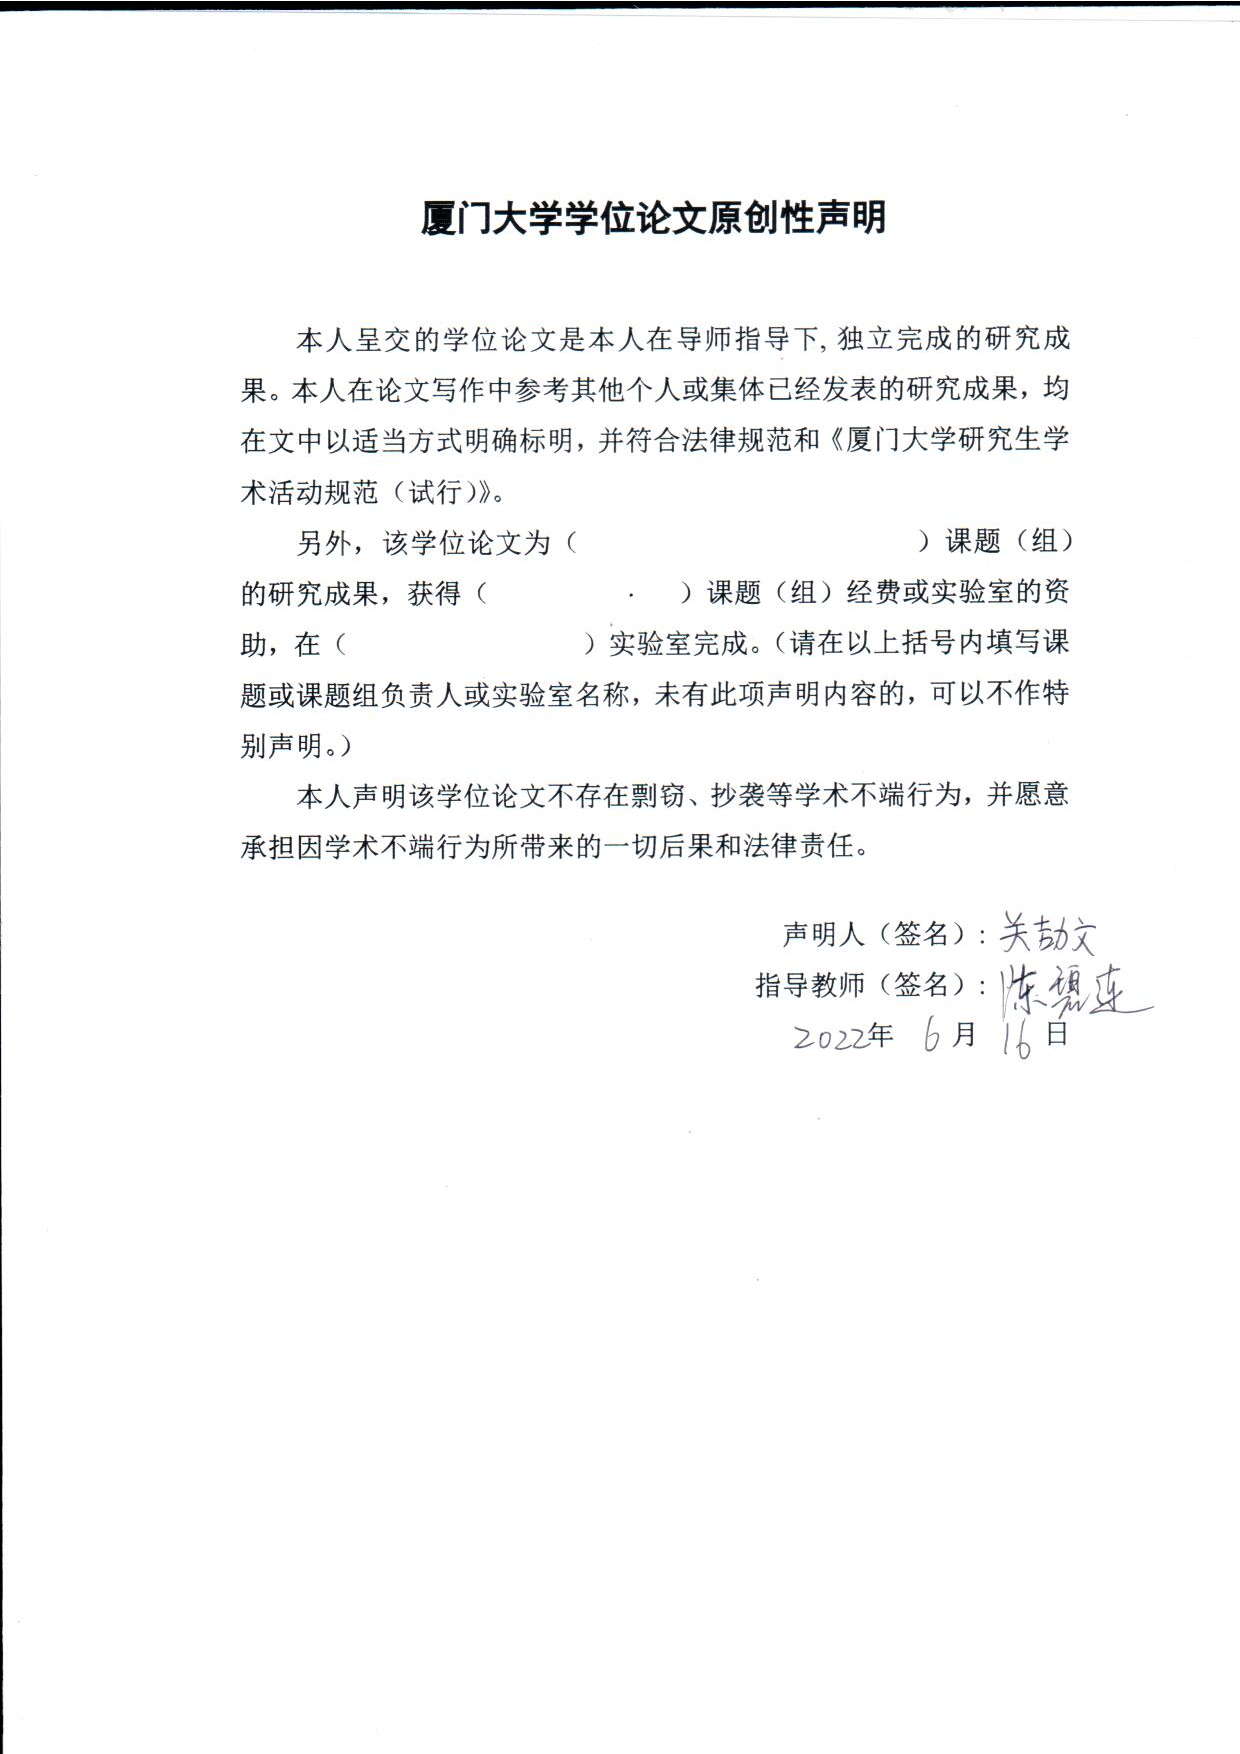
\includepdf[pages=-]{figures/yuanchuang.pdf}
%  \clearpage\cleardoublepage
\afterpage{\null\newpage}\clearpage

% \begin{center}\section*{\heiti \zihao{-2}厦门大学学位论文著作权使用声明}\end{center}
% \vspace*{21pt}
%  \par
%  本人同意厦门大学根据《中华人民共和国学位条例暂行实施办法》等规定保留和使用此学位论文,并向主管部门或其指定机构送交学位论文(包括纸质版和电子版),允许学位论文进入厦门大学图书馆及其数据库被查阅、借阅。本人同意厦门大学将学位论文加入全国博士、硕士学位论文共建单位数据库进行检索,将学位论文的标题和摘要汇编出版,采用影印、缩印或者其它方式合理复制学位论文。
%  \par
%  本学位论文属于:
%  \par
%  \thinspace(\hspace{3em})1.经厦门大学保密委员会审查核定的保密学位论文,于\quad \qquad 年\qquad 月\qquad 日解密,解密后适用上述授权。
%  \par
%  \thinspace(\hspace{3em})2.不保密,适用上述授权。
%  \par
%  (请在以上相应括号内打“\checkmark”或填上相应内容。保密学位论文应是已经厦门大学保密委员会审定过的学位论文,未经厦门大学保密委员会审定的学位论文均为公开学位论文。此声明栏不填写的,默认为公开学位论文,均适用上述授权。)
%  \vspace{3ex}
%  \par \hfill
%  声明人(签名):~~~~~~~~~~~~
%  \par \hfill
%  年~~~~~~~~月~~~~~~~~~日
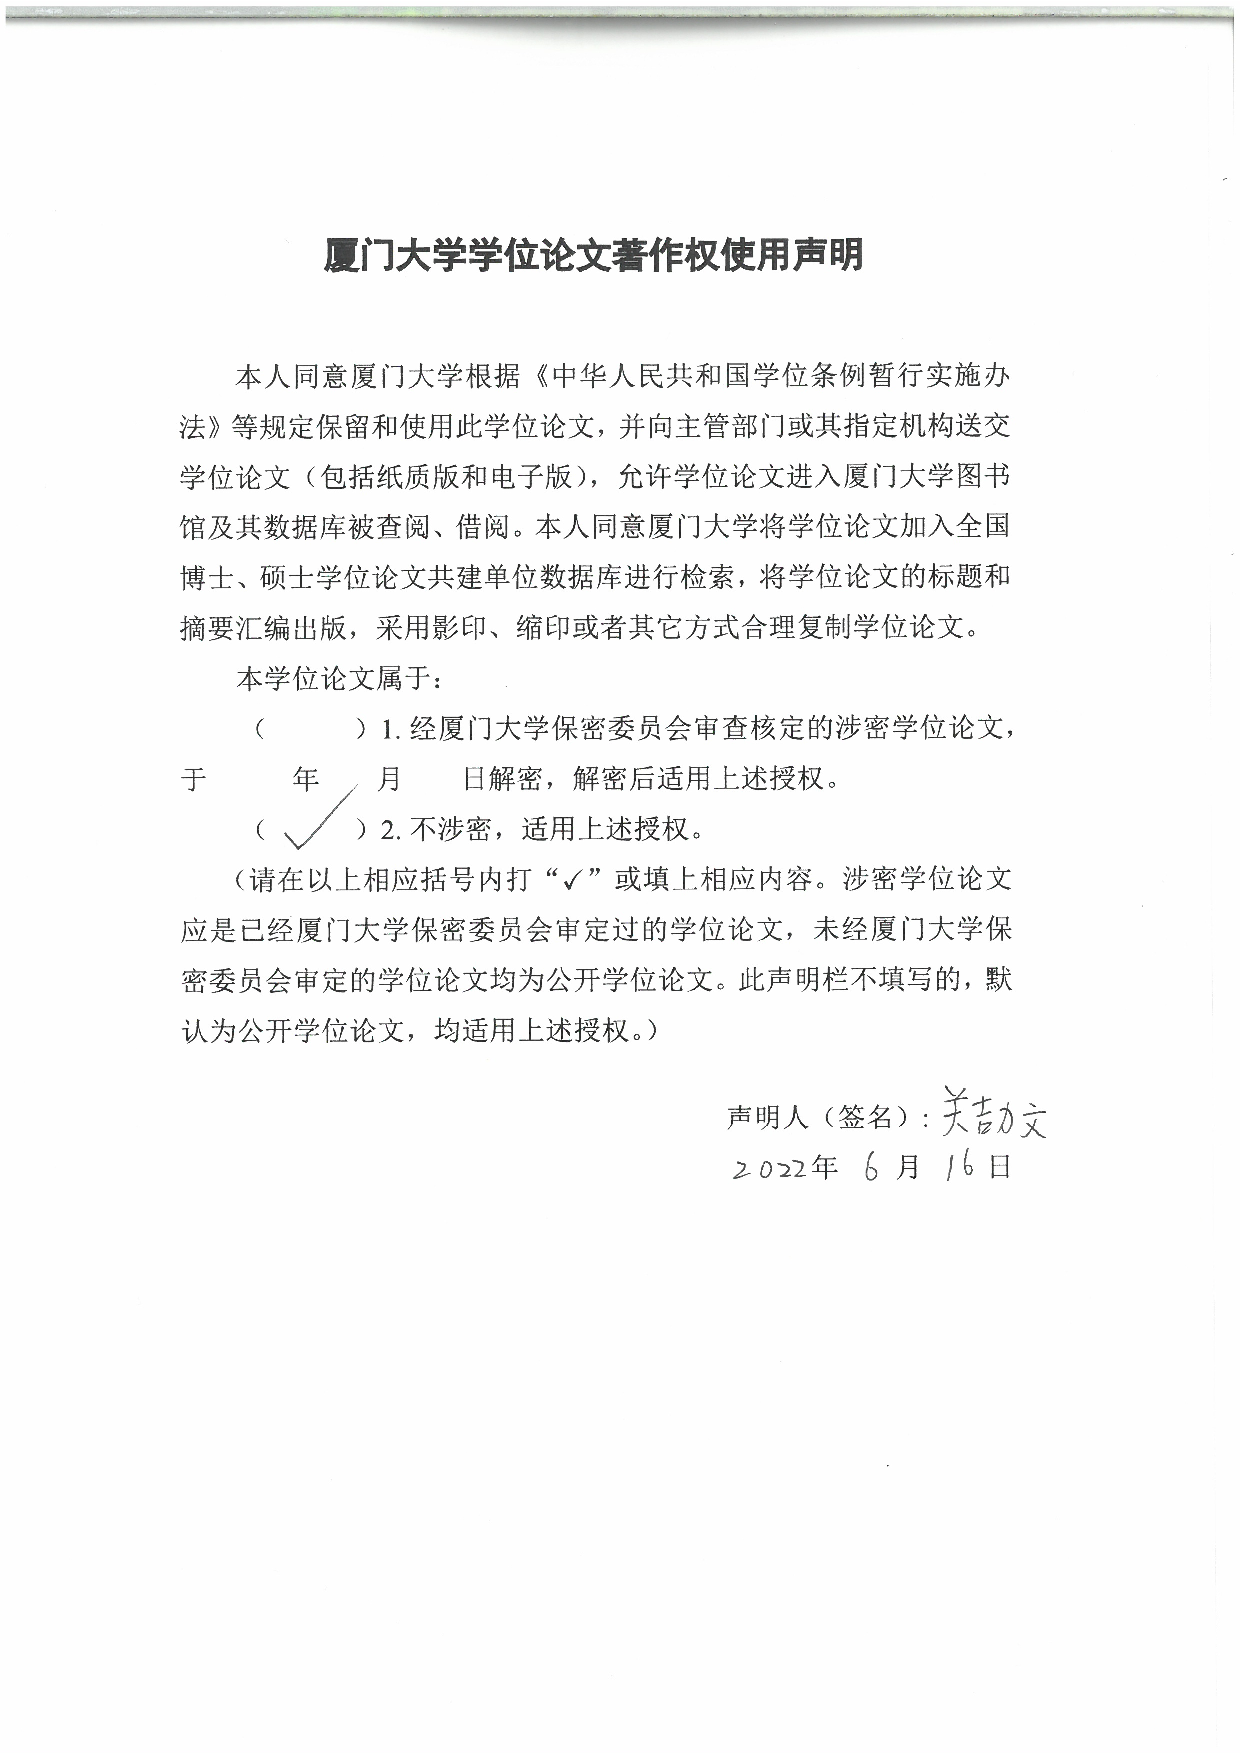
\includepdf[pages=-]{figures/zhuzuo.pdf}
\afterpage{\null\newpage}\clearpage
\zihao{-4}
%摘要
%# -*- coding:utf-8 -*-
\pagenumbering{Roman} %定义页码格式为罗马字母
\begin{cabstract}
    无监督特征选择与提取是现代数据分析不可或缺的一部分。尽管经过二十余年的发展,这些技术已经较为成熟,但它们仍在一些方面存有改进空间。例如,几乎所有现有的无监督特征选择方法都是基于矩阵优化的,而这样的框架损失了张量型数据内在的结构信息;许多现有的基于张量优化的无监督特征提取方法都没有内置的抗噪声机制,而这将导致它们在面对不确定数据时的性能退化。为了突破上述限制,本文提出了新颖且有效的基于张量优化的无监督特征选择与鲁棒特征提取方法。具体贡献如下:
    \begin{enumerate}[wide]
        \item 对于无监督特征选择任务,本文首先提出了基于非负张量CANDECOMP/\linebreak PARAFAC(CP)分解的无监督特征选择方法(Nonnegative Tensor CP Decom-position-Based Unsupervised Feature Selection, CPUFS)。CPUFS方法开创性地采用了张量CP分解来生成数据伪标签,并设计了崭新的面向张量的线性分类器、特征选择矩阵以及基于$\ell_{2,1}$范数和Khatri-Rao积的特征选择机制来进行特征选择,从而能够在整个无监督特征选择的过程中都全然保留张量的结构信息。
        % 这在本文作者的知识体系内是前所未有的。
        在CPUFS方法的基础上,本文还提出了一个对其线性分类器施加非负约束的变体,将其推广到了更高阶形式。
        % 本文还提出了基于非负张量CP分解的非负无监督特征选择方法(Nonnegative Tensor CP Decomposition-Based Nonnegative Unsupervised Feature Selection, CPUFSnn)。CPUFSnn方法在CPUFS方法的基础上为线性分类器施加了非负约束,从而能进一步利用数据的非负特性提升特征选择的性能。
        \item 对于无监督特征提取任务,本文分别提出了基于$\ell_{1}$范数和$\ell_{\infty}$范数的鲁棒张量Tucker分解的两种方法($\ell_{1}$方法和$\ell_{\infty}$方法)。$\ell_{1}$方法将所有数据样本的Tucker分解拟合误差之和作为其目标函数,从而在一定程度上抑制了数据中的噪声及离群点所带来的负面影响。$\ell_{\infty}$方法将所有数据样本的最大Tucker分解拟合误差作为其目标函数,从而更进一步地提升了在噪声环境下的特征提取的鲁棒性。
    \end{enumerate}
    
    对于这些提出的方法,本文分别研发了高效的优化算法,并从理论上进行了收敛性与计算复杂度分析。在大量真实世界基准数据集上进行了广泛且丰富的实验,实验结果表明所提出方法比前沿方法更具优越性和有效性。
    
\keywords{\mbox{特征选择;特征提取;张量计算;最优化理论;算法设计}}
\end{cabstract}

\begin{eabstract}
% \setstretch{1.0}
Unsupervised feature selection and extraction are vital and indispensable parts of modern data analytics. Although these techniques have been well developed in the recent two decades, there is still room for improvement. As examples, almost all existing unsupervised feature selection methods are matrix optimization-based, which destroy the multi-dimensional structure of tensor data; many existing tensor optimization-based unsupervised feature extraction methods do not admit built-in anti-corruption mechanisms, leading to poor performance under noisy environments. To dismiss the above-mentioned limitations, this dissertation proposes novel and effective tensor optimization-based unsupervised feature selection and robust extraction methods. The main contributions of the dissertation are summarized as follows:
\begin{enumerate}[wide]
    \item For unsupervised feature selection, this dissertation first proposes the Nonnegative Tensor CANDECOMP/PARAFAC (CP) Decomposition-Based Unsupervised Feature Selection (CPUFS) method. Specifically, CPUFS innovatively adopts the nonnegative tensor CP decomposition to generate pseudo-labels for data, and designs new tensor-oriented linear classifier, feature selection matrix and $\ell_{2,1}$-norm- and Khatri-Rao product-based feature selection mechanism to perform feature selection.
    % , which are unprecedented to the best of the author's knowledge.
    As a result, CPUFS is capable to preserve the structural information of tensor data in the whole feature selection process. 
    In addition, this dissertation proposes a variant of CPUFS which imposes nonnegativity constraints on the linear classifier, and also extends CPUFS to higher-order cases.
    % the Nonnegative Tensor CP Decomposition-Based Nonnegative Unsupervised Feature Selection (CPUFSnn) method. On top of CPUFS, CPUFSnn imposes additional nonnegativity constraints on the linear classifier so as to further improve the performance of feature selection by exploiting the nonnegative nature of data.
    
    \item For unsupervised feature extraction, this dissertation proposes two robust nonnegative tensor Tucker decomposition methods based on $\ell_{1}$-norm and $\ell_{\infty}$-norm respectively ($\ell_{1}$ and $\ell_{\infty}$ method). The $\ell_{1}$ method computes the sum of fitting errors of Tucker decomposition of all data samples as its objective function, so as to impair the negative effects caused by noise and outliers in data. Furthermore, the $\ell_{\infty}$ method computes the largest fitting error of Tucker decomposition among all data samples as its objective function, so as to further increase the robustness of feature extraction under noisy environments.
\end{enumerate}
For these proposed methods, efficient optimization algorithms are respectively developed, and theoretical analyses on their convergence and computational complexity are also conducted. Extensive and comprehensive experiments are performed on a variety of real-world benchmark datasets, in comparison with the state-of-the-arts, and the results demonstrate the superiority and effectiveness of the proposals.

\ekeywords{Feature Selection; Feature Extraction; Tensor Computation; Optimization Theory; Algorithm Design}
\end{eabstract}

% [wide, labelwidth=!, labelindent=0pt]

%生成中文目录
\tableofcncontents
\afterpage{\null\newpage}\clearpage
%生成英文目录
\tableofengcontents

\pagenumbering{arabic} %设置页码显示格式
%章节
%# -*- coding:utf-8 -*-
\chapter{绪论}\label{chap:intro}
\echapter{Introduction}
\section{研究背景}
\esection{Research Backgrounds}
统计学习方法\ucite{李航2012统计学习方法}是当下研究的热点问题。此外,它还对人类社会的发展产生了极大的推动作用。例如,手写体识别技术\ucite{lecun1989handwritten}帮助人类得以借助机器来实现在各个领域的自动化;压缩感知技术\ucite{candes2005decoding}帮助人类高效且低损耗地在计算机中保留真实世界的信息。统计学习方法旨在从数据中学习。由于数据获取技术的高速发展,当下实际应用中的数据维度越来越高。然而, 高维数据分析中一个棘手且无法回避的问题就是所谓的“维度诅咒”\ucite{bellman1966dynamic}:随着数据维度的增高,统计学习的难度将会越来越大,且性能将会越来越差。作为阐释性的引子,考虑以下引理及例子(对于此处使用到的符号,请读者参考\refsection{sec:notation})。
\begin{lemma}[Beyer等人\ucite{beyer1999nearest}]\label{lemma:highdim}\kaishu
考虑由$n$个$d$维样本点组成的数据集$\mathcal{D}=\{\boldsymbol{x}_{:1},\allowbreak\boldsymbol{x}_{:2},\ldots,\allowbreak\boldsymbol{x}_{:n}\}\subseteq\mathbb{R}^{d}$,其中$\boldsymbol{x}_{:i}$从任意数据分布$\mathcal{F}$采样,$\forall~ i=1,2,\ldots,n$。设$\boldsymbol{q}\in\mathbb{R}^{d}$为$d$维空间中的任意一点。若$\forall~ i=1,2,\ldots,n$,$\lim_{d\rightarrow\infty}\mathbb{V}\left(\frac{\norm{\boldsymbol{x}_{:i}-\boldsymbol{q}}_{2}}{\mathbb{E}\left(\norm{\boldsymbol{x}_{:i}-\boldsymbol{q}}_{2}\right)}\right)=0$,
% \begin{equation*}
%     \lim_{d\rightarrow\infty}\mathbb{V}\left(\frac{\norm{\boldsymbol{x}_{:i}-\boldsymbol{q}}_{2}}{\mathbb{E}\left[\norm{\boldsymbol{x}_{:i}-\boldsymbol{q}}_{2}\right]}\right)=0,~\forall~ i=1,2,\ldots,n,
% \end{equation*}
则随着$d\rightarrow +\infty$,
\begin{equation*}
    \frac{\max_{\boldsymbol{x}\in\mathcal{D}}\norm{\boldsymbol{x}-\boldsymbol{q}}_{2}}{\min_{\boldsymbol{x}\in\mathcal{D}}\norm{\boldsymbol{x}-\boldsymbol{q}}_{2}}\rightarrow_{\mathbb{P}}1.
\end{equation*}
\end{lemma}
\reflemma{lemma:highdim}传达道,在满足某些关于数据分布$\mathcal{F}$的假设时,在超高维空间中所有$\mathcal{D}$中样本点到空间中任意点$\boldsymbol{q}$的距离都几乎是相等的!在这种情况下,$k$近邻分类器\ucite{李航2012统计学习方法}将变得极度不稳定:对$\boldsymbol{x}_{:i}$而言,所有属于$\mathcal{D}\setminus\{\boldsymbol{x}_{:i}\}$的点都几乎是他的最近邻点——这是无意义的。除此之外,高维数据还会来带诸如组合数爆炸\ucite{靳志宏2008物流调度与协调},影响数值计算效率等诸多不良问题,坏处多多。本节再通过以下例子来更加直观地体会高维数据对统计学习带来的负面影响。

% [Amini\ucite{200c}]
\begin{example}\label{ex:highdim-reg}\kaishu
    考虑由$n$个$d$维样本点组成的数据集$\mathcal{D}=\{(\boldsymbol{x}_{:1},y_{1}),\allowbreak\ldots,\allowbreak(\boldsymbol{x}_{:n},y_{n})\}\subseteq\mathbb{R}^{d}\times\mathbb{R}$,以及如下带噪声的线性回归模型$y_{i}=\bm{\beta}^{\top}\boldsymbol{x}_{:i}+w_{i}$,其中$y_{i}\in\mathbb{R}$为第$i$个样本的观测值,$\bm{\beta}\in\mathbb{R}^{d}$为回归参数向量,$\boldsymbol{x}_{:i}\in\mathbb{R}^{d}$为第$i$个样本的特征,而$w_{i}\sim\mathcal{N}(0,1)$为对应于第$i$个样本的标准高斯噪声。假设$n\gg d$,则从数据$\mathcal{D}$中学习回归参数向量$\bm{\beta}$的有效方法为最小二乘法,即如下优化问题
    \begin{equation*}
        \begin{aligned}
            &\underset{\bm{\beta}}{\min}&& \norm{\boldsymbol{X}^{\top}\bm{\beta}-\boldsymbol{y}}_{2}^{2}.
        \end{aligned}
    \end{equation*}
    上述优化问题为光滑凸优化问题,并且它有显式最优解
    \begin{equation*}
        \hat{\bm{\beta}}=\parenth{\boldsymbol{X}\boldsymbol{X}^{\top}}^{-1}\boldsymbol{X}\boldsymbol{y}.
    \end{equation*}
    然而,在高维情形时(即$d>n$),上述问题将急剧恶化。例如,由于在求最优解时需要对矩阵$\boldsymbol{X}\boldsymbol{X}^{\top}\in\mathbb{R}^{d\times d}$求逆,但是在$d>n$时,$\operatorname{rank}(\boldsymbol{X}\boldsymbol{X}^{\top})\leq n<d$,因而$\boldsymbol{X}\boldsymbol{X}^{\top}$不再可逆!故无法再利用上式求解!此外,哪怕对于无噪声情形(即$w_{i}$恒为$0$),也无法求得最优的参数,原因如下。在无噪声情形下,需要求解如下线性方程组
    \begin{equation*}
        \left\{
        \begin{aligned}
            y_{1} &= x_{11}\beta_{1}+x_{21}\beta_{2}+\ldots+x_{d1}\beta_{d},\\
            y_{2} &= x_{12}\beta_{1}+x_{22}\beta_{2}+\ldots+x_{d2}\beta_{d},\\
            &\vdotswithin{=}\\
            y_{n} &= x_{1n}\beta_{1}+x_{2n}\beta_{2}+\ldots+x_{dn}\beta_{d}.
        \end{aligned}
        \right.
    \end{equation*}
    然而,由线性代数理论\ucite{丘维声2002高等代数},上述线性方程组是欠定的,因为它其中的决策变量个数$d$大于方程的个数$n$。这也就导致了上述线性方程组有无穷多解。真正的回归参数向量$\bm{\beta}^{*}$不可能从无穷多个解中被辨识出。
\end{example}

为了缓解高维特征带来的各种问题,特征选择与提取技术发挥了重要作用。特征选择旨在从高维特征中原封不动地选择出高质量的特征子集(通常基数很小),并同时滤除原有特征中的噪声及冗余;而特征提取旨在将原有的高维特征通过线性或非线性变换投影至低维子空间,并使得这些低维的数据表示可以很好地反应原有的数据特征,从而实现特征降维。这些降维技术削弱了“维度诅咒”的影响,从而为高维数据分析提供了极大的便利。特征选择与提取方法可以进一步分为三大类:有监督、半监督以及无监督特征选择与提取\ucite{solorio2020review,ang2015supervised,ghojogh2019feature}。在这其中,由于无监督特征选择与提取不需要使用数据中的标签作为引导,因而具有更广的适用性,但作为代价也更具挑战性。本文关注于无监督特征选择与提取问题。下面两节将分别介绍它们的相关背景。

\subsection{无监督特征选择研究背景}
\esubsection{Research Backgrounds of Unsupervised Feature Selection}
无监督特征选择旨在在没有数据标签引导的情况下实现数据特征子集的高质量选取。进一步地,无监督特征选择方法可以再分为以下三种类型\ucite{综述1,综述2,综述3}:
\begin{enumerate}
    \item \textbf{包裹式:}包裹式特征选择方法旨在通过学习器来评估选择出来的特征的优劣程度,从而选择出针对某个学习器而言的最佳特征子集。
    % 具有代表性的包裹式特征选择方法为递归特征消除\ucite{RFE}。递归特征消除通过在数据上训练学习器来从特征集合中筛选出相对于该学习器作用最大的特征,并将它从特征集合中消除,并继续在其余特征子集上重复上述过程,从而得到一个特征排序。但由于每一次评价特征子集都需要训练一次学习器,递归特征消除的计算花费会比较大。
    \item \textbf{嵌入式:}嵌入式特征选择方法旨在在模型学习的过程中融合进特征选择,从而使得被选择的特征可以更好地适应某个学习模型。
    % 具有代表性的嵌入式特征选择方法为最小绝对值收敛和选择算子\ucite{LASSO}。最小绝对值收敛和选择算子在最小二乘回归的目标函数上还融合了一项参数向量的$\ell_{1}$范数,从而实现了在最小二乘的过程中自动地进行特征选择。
    \item \textbf{过滤式:}过滤式特征选择方法旨在直接根据数据的内在特性来选择高质量的特征,且被选择的特征与下游学习模型无关。
    % 具有代表性的过滤式特征选择方法为方差过滤法\ucite{varthre},即直接过滤掉那些方差较低的特征(或直接筛选出那些方差较高的特征)。方差过滤法的工作原理为,对于那些方差较小的特征,由于它们在不同样本之间的差异不明显导致它们不具有较强的判别性,从而应被视为冗余而滤去。此外,我们还可以从互信息\ucite{richert2013building}等其它角度来进行过滤式特征选择。
\end{enumerate}

从以上介绍中可以看到,相比于包裹式与嵌入式方法,过滤式方法直接通过数据的内在特性来选择特征,而非利用额外的学习器来评价被选择特征的质量或将特征选择融合进某个额外的学习器里,从而具有非常大的便利性以及更广的适用性。这样的优点使得过滤式无监督特征选择受到广泛的应用。下文将主要关注过滤式无监督特征选择。

由于张量的大规模普及,开发面向张量的无监督特征选择方法成为了重要的任务。然而,遗憾的是,业内几乎找不到任何面向张量的无监督特征选择方法。本文旨在研发一套完善的基于张量优化的无监督特征选择方案,从而填补业内在面向张量的无监督特征选择这一领域的空白。

\subsection{无监督特征提取研究背景}
\esubsection{Research Backgrounds of Unsupervised Feature Extraction}
无监督特征提取旨在在没有数据标签引导的情况下实现数据特征的高质量提取。由于张量的大规模普及,开发面向张量的无监督特征提取方法成为了重要的任务。与无监督特征选择不同,近年来,业内已经出现了一系列基于张量优化的无监督特征提取方法。主要地,非负张量Tucker分解\ucite{kolda2009tensor}常常作为这些方法的骨干模型出现,其中核心张量被视为被提取的低维特征。此外,基于张量优化的无监督特征提取还可以从张量主成分分析\ucite{lu2008mpca,lu2016tensor}与张量填充\ucite{ferlrtc}等角度出发研究。相比于基于矩阵优化的无监督特征提取方法,基于张量优化的无监督特征提取方法能够保留住张量中的结构信息,从而具有更好的效果。下文将主要关注基于张量优化的无监督特征提取。

然而,在这些基于张量优化的无监督特征提取方法中,很少有方法关注到数据不确定性所带来的负面影响。在现实应用场景中,高维数据往往带有噪声和离群点,并且这些噪声和离群点会对特征提取的性能产生较大影响。因此不得对这些噪声与离群点坐视不管。此外,尽管有少数方法已经具备内置的抗噪机制,但它们仍然存在改进空间。本文旨在研发更加鲁棒的基于张量优化的无监督特征提取方法,从而进一步提升在噪声场景下的张量无监督特征提取的效果。

\section{相关工作与研究现状}
\esection{Related Work and Research Status}
本节将介绍无监督特征选择方法以及基于张量优化的特征提取方法
% \footnote{由于基于张量优化的特征提取工作数量较少,为了综述的充分性,我们在这一节综述的这些工作既包括了无监督的,也包括了有监督的。}
。
\subsection{无监督特征选择研究综述}\label{sec:review-ufs}
\esubsection{Research Review for Unsupervised Feature Selection}
本节将介绍无监督特征选择。首先介绍过滤式无监督特征选择方法,这些方法在过去的十年内是业内的研究热点与焦点;之后介绍当前业内唯一可考的基于张量优化的嵌入式无监督特征选择方法。

% 具体而言,如果某一个特征在相似的样本点上差异不大,但是在相异的样本点上有较大差异,那么这个特征将会被认为有很高的判别性。

近十年来,过滤式无监督特征选择技术在业内得到了很好的发展。这一领域具有代表性的工作综述如下。在无监督特征选择发展早期,He等人\ucite{lapscore}提出拉普拉斯评分法(Laplacian Score, LapScore),其通过评估各个特征保留数据局部几何结构的能力高低来进行特征选择;为了更好地保留数据的多簇结构特征,Cai等人\ucite{cai2010unsupervised}提出多簇特征选择方法(Multi-Cluster Feature Selection, MCFS),其首先通过谱分析来获得数据的内在聚类结构,而后使用基于$\ell_{1}$范数的稀疏回归来进行特征选择。随后,Nie等人\ucite{nie2010efficient}提出使用$\ell_{2,1}$范数对特征选择矩阵施加行稀疏正则,并开发了可证明收敛性的高效优化算法,从此掀起了基于$\ell_{2,1}$范数的特征选择方法的研究热潮。例如,Yang等人\ucite{udfs}在局部判别分析以及基于$\ell_{2,1}$范数的特征选择的基础上提出了无监督判别特征选择方法(Unsupervised Discriminative Feature Selection, UDFS),从而来选择那些最具判别性的特征;Hou等人\ucite{jelsr}在局部线性近似、稀疏回归以及基于$\ell_{2,1}$范数的特征选择的基础上提出了联合嵌入学习和稀疏回归的特征选择方法(Feature Selection via Joint Embedding Learning and Sparse Regression, JELSR),从而能更好地捕获数据的局部结构信息;Li等人\ucite{ndfs}在非负谱分析、伪标签回归以及基于$\ell_{2,1}$范数的特征选择的基础上提出了非负判别特征选择方法(Nonnegative Discriminative Feature Selection, NDFS),从而很好地利用了数据的局部结构信息及其非负本质来引导特征选择。为了进一步提升无监督特征选择在带噪声环境下的鲁棒性,Qian等人\ucite{rufs}在鲁棒非负矩阵分解\ucite{kong2011robust}、线性伪标签回归以及基于$\ell_{2,1}$范数的特征选择的基础上提出了鲁棒无监督特征选择方法(Robust Unsupervised Feature Selection, RUFS),从而能很好地应对数据中的噪声和离群点;Shi等人\ucite{rsfs}在谱分析、鲁棒谱回归以及基于$\ell_{2,1}$范数的特征选择的基础上提出了鲁棒谱分析无监督特征选择方法(Robust Spectral Analysis for Unsupervised Feature Selection, RSFS),从而能进一步提升特征选择的鲁棒性。此外,为了充分利用数据聚类信息,Han等人\ucite{socfs}在正交基聚类以及基于$\ell_{2,1}$范数的特征选择的基础上提出了同步正交基聚类与特征选择方法(Simultaneous Orthogonal Basis Clustering and Feature Selection, SOCFS),从而能够利用聚类中心实现更好的特征选择。在所有上述方法中,数据的局部结构信息(若有使用到)都为预先计算,而非通过对数据进行自适应学习得到。为了弥补这个缺陷,Du等人\ucite{fsasl}在数据的自适应相似度图学习以及基于$\ell_{2,1}$范数的特征选择的基础上提出了自适应结构学习无监督特征选择方法(Unsupervised Feature Selection with Adaptive Structure Learning, FSASL),从而能够自适应地捕获数据的局部结构信息;Nie等人\ucite{sogfs}基于与FSASL方法近乎同样的架构提出了结构图优化无监督特征选择方法(Structured Optimal Graph Feature Selection, SOGFS);Li等人\ucite{urafs}在无关联回归、基于最大熵的数据自适应相似度图学习以及基于$\ell_{2,1}$范数的特征选择的基础上提出了基于广义无关联回归和自适应图的特征选择方法(Generalized Uncorrelated Regression with Adaptive Graph for Unsupervised Feature Selection, URAFS),从而能选择那些具有判别性但近乎无关的特征。此外,Zhu等人\ucite{cdlfs}另辟蹊径,提出了耦合字典学习无监督特征选择方法(Coupled Dictionary Learning for Unsupervised Feature Selection, CDLFS),其通过字典学习来重构数据,并使用字典学习模型的表示参数来建模数据分布,最后通过数据分布来选择特征;Guo等人\ucite{dgufs}在特征选择以及基于被选择特征的数据聚类的基础上提出了相关性引导的无监督特征选择方法(Dependence Guided Unsupervised Feature Selection, DGUFS),从而提升了数据、产生的伪标签以及被选择的特征三者之间的相关性。除了使用$\ell_{2,1}$范数以外,其它具有与$\ell_{2,1}$范数相似功能但性质更好的(拟)范数也被采用至无监督特征选择。例如,Nie等人\ucite{nie2020unsupervised}在数据的自适应相似度图学习以及基于$\ell_{2,0}$范数的特征选择的基础上提出了基于行稀疏约束和最优图的无监督特征选择方法(Unsupervised Feature Selection with Row-Sparsity Constraint and Optimized Graph, RSOGFS),从而进一步提升特征选择的精准度;Li等人\ucite{li2021sparse}受到主成分分析\ucite{wold1987principal}的启发提出了基于稀疏主成分分析的特征选择方法(Sparse Principal Component Analysis for Feature Selection, SPCAFS),其通过对主成分分析的投影矩阵施加基于$\ell_{2,p}$范数的稀疏正则来实现特征选择。

然而,所有上述方法都是基于矩阵优化的。尽管它们实现起来都相对容易,然而作为代价,所有这些方法都会丢失张量的内在结构信息(因为它们会将张量向量化从而使得它们可处理)。这对于特征选择而言是不利的。
% 相比之下,我们所提出的CPUFS方法采用了非负张量CP分解用于生成伪分类标签,并利用针对张量量身定制的线性分类器和特征选择矩阵来进行伪标签回归以及特征权重稀疏化,从而在整个特征选择过程中都全然保留了张量中的结构信息。
本节接下来介绍当前业内唯一可考的基于张量优化的无监督特征选择方法。Su等人在低秩张量表示学习、数据的自适应相似度图学习以及基于$\ell_{2,1}$范数的特征选择的基础上提出了基于图正则的低秩张量表示方法(Graph Regularized Low-Rank Tensor Representation, GRLTR)。然而,尽管GRLTR是一种基于张量优化的无监督特征选择方法,但是在其具体实现中,张量的结构信息在向低维流形投影的过程中被丢失了。这是由于GRLTR在向低维流形投影时将张量展开成了矩阵,而这个过程破坏了张量的结构信息。但流形投影是其整个无监督特征选择过程中最重要的一步,因为该投影矩阵同时也是特征选择矩阵,其质量直接决定了特征选择的效果好坏。因而该方法存在一定的内在缺陷。此外,需要注意的是,GRLTR(如其文章\ucite{GRLTR}所述)为一种嵌入式无监督特征选择方法。
% 与GRLTR相对比,我们的CPUFS方法在特征选择的全过程中均保留了数据结构:我们不仅使用非负张量CP分解来对张量产生伪标签,同时还设计了新的面向线性分类器以及特征选择矩阵。这样的缜密设计使得张量的结构信息在CPUFS中得到了很好的保留。


\subsection{基于张量优化的特征提取研究综述}\label{sec:review-ufe}
\esubsection{Research Review for Tensor Optimization-Based Feature Extraction}
本节将介绍基于张量优化的特征提取。由于这些工作数量较少,因此为了综述的充分性,既综述无监督的方法,也综述有监督的方法。
% 此外,由于特征提取与特征选择具有某种程度上的相似,因而虽然本小节综述的这些方法并非面向特征选择,但它们可能会对基于张量优化的特征选择方法的研发带来深层次的启发。

% \section{\texorpdfstring{无监督特征提取中的$\ell_{1}$}{L1}与\texorpdfstring{$\ell_{2}$}{L2}模型的优化模型}
% \esection{Optimization Models of the \texorpdfstring{$\ell_{1}$}{L1} and \texorpdfstring{$\ell_{2}$}{L2} Methods in Unsupervised Feature Extraction}

本节首先综述基于张量优化的非鲁棒特征提取方法。最早的面向张量的特征提取方法大致可以追溯到Yan等人\ucite{yan2005discriminant}提出的张量表示判别分析方法(Discriminant Analysis with Tensor Representation, DATER),其将线性判别分析(Linear Discriminative Analysis, LDA)\ucite{mika1999fisher}拓展到了张量形式,从而提升了线性判别分析对于张量的特征提取效果;类似地,Lu等人\ucite{lu2008mpca}提出的多线性主成分分析方法(Multilinear Principal Component Analysis, MPCA)将经典的主成分分析\ucite{wold1987principal}推广到了张量形式,从而得以有效地从张量中提取特征;Idaji等人\ucite{2017HOSRDA}提出的高阶谱回归判别分析方法(Higher-Order Spectral Regression Discriminant Analysis, HOSRDA)将谱回归判别分析(Spectral Regression Discriminant Analysis, SRDA)\ucite{cai2007srda}拓展到了张量形式,从而能使其更好地适应张量。
% 之后,Phan和Cichocki\ucite{2010TDFE}提出对张量Tucker分解的参数矩阵施加正交或非负约束并开发了高效的求解算法。这些模型在图像数据以及脑电波数据上取得了很好的效果。
除以上的经典拓展方法以外,基于张量分解的特征提取方法也在业内受到了广泛关注,并且在近十年内得到了快速发展。例如,Jukic等人\ucite{2013MaxMutInfo}提出的基于互信息的张量分解方法(Mutual Information-Based Tensor Decomposition, MITD)将互信息最大化融合进张量分解,从而得以捕获张量中的高阶统计信息;Li等人\ucite{2016MR-NTD}在非负Tucker分解和图正则的基础上提出了基于流形正则的非负Tucker分解方法(Manifold Regularization-Nonnegative Tucker Decomposition, MR-NTD),从而能够在从张量中提取特征的同时很好地保留张量的局部几何结构信息;Ju等人\ucite{ju2017vectorial}提出的张量贝叶斯向量化降维方法(Tensor Bayesian Vectorial Dimension Reduction, TBV-DR)在贝叶斯分析的框架下将张量表示成一些具有同样阶数的张量基的线性组合,并且用这些线性组合的表示系数来作为降维后的低维数据表示;Yin和Ma\ucite{2019LELLE-NTD}提出的基于局部线性嵌入的非负Tucker分解方法(Locally Linear Embedding-Based Nonnegative Tucker Decomposition, LLE-NTD)和基于拉普拉斯特征图的非负Tucker分解方法(Laplacian Eigenmaps-Based Nonnegative Tucker Decomposition, LE-NTD)分别使用了局部线性嵌入(Locally Linear Embedding, LLE)\ucite{LLE}和拉普拉斯特征图(Laplacian Eigenmaps, LE)\ucite{LapE}作为正则项来提升非负张量Tucker分解的性能;Shi等人\ucite{2019TDVM}在张量缺失值填充以及特征方差最大化的基础上提出了基于特征方差最大化的低秩张量分解方法(Low-Rank Tensor Decomposition with Feature Variance Maximization, TDVM),从而得以在张量有缺失值的情况下仍然能从中有效地提取特征。此外,基于张量填充技术的特征提取方法也在最近取得了一系列的成功。例如,Fu等人\ucite{ferlrtc}提出的基于低秩张量填充的人脸表情识别方法(Facial Expression Recognition via Low-Rank Tensor Completion, FERLrTC)通过对张量Tucker分解的参数矩阵施加低秩正则以及对张量Tucker分解的核心张量施加稀疏正则构建了基于张量Tucker分解的低秩表示模型,并成功地将其用应于2D+3D人脸表情识别。

然而,尽管上述方法都在张量上取得了较好的效果,但是它们都没有考虑到数据中的噪声等其它因素带来的负面影响。事实上,数据噪声对特征提取的影响不容小觑。为了增强张量特征提取的鲁棒性,有少数学者提出了一些基于张量$\ell_{1}$范数或其它范数的特征提取方法,从而得以更加鲁棒地从张量中提取特征。本节接下来综述这些方法。Pang等人\ucite{L1Tucker2}提出的基于$\ell_{1}$范数的张量分析方法($\ell_{1}$-Norm-Based Tensor Analysis, TPCA-$\ell_{1}$)将广义低秩矩阵估计方法(Generalized Low Rank Approximations of Matrices, GLRAM)\ucite{ye2005generalized}(尽管该方法用于矩阵估计,但Pang等人是用一种张量的观点来看待的)中的张量Frobenius范数替换为了张量$\ell_{1}$范数,从而能较好地抑制数据中的噪声与离群点所带来的负面影响;在此基础上,Markopoulos等人\ucite{2018ExaL1Tucker}为秩-$1$情况下的TPCA-$\ell_{1}$方法设计了两种高效的优化算法;此外,类似地,Markopoulos等人\ucite{2018L1HOSVD,2020L1HOOI,2019L1Tucker}还分别将张量$\ell_{1}$范数应用到了高阶奇异值分解(Higher-Order Singular Value Decomposition, HOSVD)\ucite{de2000multilinear}以及高阶正交迭代(Higher Order Orthogonal Iteration, HOOI)\ucite{de2000best}当中,并开发了相应的优化算法;Zhang和Ding\ucite{2013RTD}提出的鲁棒张量Tucker分解方法(Robust Tucker Tensor Decomposition, RTD)将正交Tucker分解中的张量Frobenius范数替换为了张量$\ell_{1}$范数,从而提升了正交Tucker分解对数据噪声的鲁棒性;在此基础之上,Cao等人\ucite{2015RTC}成功地将RTD方法应用到了鲁棒人脸聚类当中。除上述方法外,基于鲁棒主成分分析(Robust Principal Component Analysis, RPCA)的张量特征提取方法也在最近吸引了较大的关注。例如,Lu等人\ucite{lu2019tensor}提出的张量鲁棒主成分分析方法(Tensor Robust Principal Component Analysis, TRPCA)使用张量$\ell_{1}$范数将基于矩阵优化的鲁棒主成分分析方法\ucite{cand2011robust}推广到了张量形式,从而得以剥离张量中的噪声与离群点以提升特征提取的鲁棒性;Zhou和Feng\ucite{2017ORTPCA}提出的离群点鲁棒张量主成分分析(Outlier-Robust Tensor PCA, OR-TPCA)将TRPCA方法中施加在噪声分量上的张量$\ell_{1}$范数替换为了张量$\ell_{2,1}$范数,从而进一步提升了特征提取对数据离群点的鲁棒性。最近,Chachlakis等人\ucite{chachlakis2021dynamic}在基于张量$\ell_{1}$范数的增量式张量Tucker分解的基础上提出了动态$\ell_{1}$-Tucker方法(Dynamic $\ell_{1}$-Tucker, D-$\ell_{1}$-Tucker),其优势在于能够在处理数据流形式的张量时很好地抑制数据中的噪声与离群点所带来的负面影响。
% 总体而言,这类鲁棒特征提取的文献仍较少。

% 然而,尽管本小节综述的模型相比前一小节的更为鲁棒,然而它们或多或少仍然存在改进空间。例如,许多模型采用张量$\ell_{1}$范数来抑制数据噪声。而$\ell_{1}$范数分配给不同样本点的权重其实是相同的。直观上来讲,我们应该更关注于那些拟合误差较大的样本。

% 除了基于张量Tucker分解以外,张量特征提取还可以从其它角度出发进行实现,例如高阶判别分析\ucite{yan2005discriminant,zhou2018probabilistic,zhang2011tensor,tao2008tensor,tao2017tensor}(拓展线性判别分析(LDA)\ucite{mika1999fisher}至张量形式),高阶主成分分析\ucite{lu2008mpca,shi2015semi,lu2016tensor,lu2019tensor,fan2014modified}(拓展主成分分析(PCA)\ucite{wold1987principal}至张量形式),张量填充\ucite{liu2012tensor,jain2014provable,liu2015generalized,liu2014trace,zhao2015bayesian,hu2016twist,han2018generalized}(拓展矩阵填充\ucite{candes2009exact}至张量形式)等等。但由于这些方法与本文提出的算法并不具有较强的联系,我们这里不再做详细的综述。

\section{研究动机、内容及贡献}\label{sec:motivation}
\esection{Research Motivation, Contents and Contributions}
本节介绍本文的研究动机所在,以及阐述研究的主要内容与贡献。
\subsection{基于张量优化的无监督特征选择}\label{sec:motiv-ufs}
\esubsection{Tensor Optimization-Based Unsupervised Feature Selection}
随着数据采集技术的进步,张量以各种形式,例如图像、视频、社交网络、功能磁共振成像以及多通道脑电图等等,广泛地出现在了各种现实应用场景中。张量天然带有结构信息,并且这些信息或会对无监督特征选择带来帮助。尽管如此,由\refsection{sec:review-ufs}中的相关工作综述中可以看到,几乎所有的无监督特征选择方法都是基于矩阵优化的。然而,这样的方法将会作为预处理的一部分将张量向量化,然后在已向量化的数据上进行特征选择。这样的做法虽然能带来模型与优化的简易性,但是作为代价,张量天然带有的数据结构也就被破坏了。除此之外,文献中几乎无法找到基于张量优化的无监督特征选择方法,并且业内唯一可考的该类型方法GRLTR\ucite{GRLTR}又存在一定的内在缺陷。因而,开发一套完善的基于张量优化的无监督特征选择方案迫在眉睫。
% 尽管如此,

为了突破上述限制,本文另辟蹊径,首先提出了基于非负张量CP分解的无监督特征选择方法(Nonnegative Tensor CP Decomposition-Based Unsupervised Feature Selection, CPUFS)。CPUFS方法可以实现从三阶张量无监督地选择特征并能完好地保留其内在结构,并且CPUFS方法可以被很容易地扩展到更高阶形式(本文将在\refsection{sec:CPUFS-extend}具体阐释拓展的方法)。具体贡献如下:
\begin{enumerate}
    \item 在方法设计方面,本文采用了基于图正则\ucite{cai2010graph}的非负张量CP分解技术\ucite{carroll1970analysis}来为张量产生伪标签,并设计了新颖的面向张量的线性分类器、特征选择矩阵以及特征选择机制。以这种方式,在整个特征选择的全过程中,张量的结构信息都被完好地保留了下来。
    \item 在求解所提出的CPUFS方法方面,本文提出了一种具有理论收敛性保证的高效迭代优化算法。除此之外,该优化算法的计算复杂度与特征数量仅呈线性关系,从而保证了整个特征选择过程的效率。
    \item 为了进一步利用输入张量和生成的伪标签的非负性,本文还提出了CPUFS方法的变体——基于非负张量CP分解的非负无监督特征选择方法(Nonnegative Tensor CP Decomposition-Based Nonnegative Unsupervised Feature Selection, CPUFSnn)。CPUFSnn方法对线性分类器施加了非负约束,从而能够利用输入张量和伪标签的非负本质进一步提升无监督特征选择的性能。
    \item 在实验部分,本文在十个真实世界基准数据集中测试了CPUFS和CPUFSnn方法,并与前沿的无监督特征选择方法进行比较。实验结果表明,CPUFS和CPUFSnn方法优于前沿的无监督特征选择方法,并展现了显著的性能提升。此外,本文还研究了CPUFS方法的参数灵敏度、运行时间、收敛速度以及其所选特征的分布情况。
    % 与\refsection{sec:review-ufs}中综述的方法相比,CPUFS和CPUFSnn方法在整个特征选择过程中都全然保留了张量中的结构信息。这是其优势所在。
\end{enumerate}
% \begin{enumerate*}[label=(\arabic*)]
% % \begin{enumerate}
%     \item \textbf{我们采用了基于图正则\ucite{cai2010graph}的非负张量CP分解技术\ucite{carroll1970analysis}来为张量产生伪标签。}由于采用了非负张量CP分解来产生伪标签,张量的数据结构被很好的保留了下来。此外,根据图正则理论\ucite{cai2010graph},在几何结构上相似的数据样本的伪标签将被图正则迫使至尽可能保持一致,而这进一步提升了伪标签的质量。
%     \item \textbf{我们设计了新颖的面向张量的线性分类器和特征选择矩阵,以在实现伪标签回归和特征选择的同时保留张量的数据结构。}新设计的线性分类器具有多个参数矩阵,并且它被直接定义在原始的张量上(而非向量化后的向量数据上),从而完好地保留了张量的数据结构。相应地,新设计的特征选择矩阵直接基于新设计的线性分类器设计,从而继承了线性分类器中所保留的数据结构信息。
% \end{enumerate*}

    % 采用了非负张量CP分解用于生成伪分类标签,并利用针对张量量身定制的线性分类器和特征选择矩阵来进行伪标签回归以及特征权重稀疏化,从而
    % 此外,与GRLTR\ucite{GRLTR}相对比,我们的CPUFS方法在特征选择的全过程中均保留了数据结构:我们不仅使用非负张量CP分解来对张量产生伪标签,同时还设计了新的面向线性分类器以及特征选择矩阵。这样的缜密设计使得张量的结构信息在CPUFS中得到了很好的保留。

% 在我们的知识范围内,这是基于张量分解技术的无监督特征选择的第一个工作。尽管从基于矩阵优化的无监督特征选择扩展到基于张量优化的无监督特征选择看似是直接且平凡的,但由于以下原因,这其中的挑战性远非寻常。
% \begin{enumerate*}[label=(\arabic*)]
%     \item \textbf{在整个特征选择过程的每个部分中都保留张量的结构信息并非易事}。一个小部分中不经意间的疏忽就会直接导致不必要的信息损失\footnote{例如在\refsection{sec:review-ufs}综述到的基于图正则的低秩张量表示方法\ucite{GRLTR}就忽略了在向流形投影的过程中保留张量的结构信息,并因此丢掉了有用的信息。}。我们认识到了在整个特征选择过程的每个部分中都保留张量的结构信息的重要性和必要性,并因此采用了非负张量CP分解以及提出了新的面向张量的线性分类器和特征选择矩阵来实现这件事。
%     \item \textbf{线性分类器的设计需要仔细斟酌}。不同于现有的方法(即,将张量向量化后进行伪标签回归),我们设计了一种新的面向张量的线性分类器。该线性分类器直接在张量上定义,并包含多个参数矩阵,从而可以保留下张量的数据结构信息。
%     \item \textbf{特征选择矩阵的设计具有很大的挑战性}。如上所述,新设计的线性分类器包含多个参数矩阵。因此,我们希望我们的特征选择矩阵能够实现
%     \begin{enumerate*}
%         \item 将这些参数矩阵都集成在一起,
%         \item 继承这些参数矩阵中保留的张量的结构信息,以及
%         \item 作为用以排序特征的特征重要性权重。
%     \end{enumerate*}
%     这是一个很难的问题。为了解决这个难题,我们设计了新的面向张量的特征选择矩阵来实现上述三点。此外,我们设计的特征选择矩阵可以被轻松地扩展到更高阶形式。
% \end{enumerate*}

\subsection{基于张量优化的鲁棒无监督特征提取}
\esubsection{Tensor Optimization-Based Robust Unsupervised Feature Extraction}
透过\refsection{sec:review-ufe}的相关工作综述可以发现,与无监督特征选择不同,对于面向张量的无监督特征提取,业内已经有许多较好的解决方案。然而,大多数方法并没有考虑到数据中的噪声与离群点所带来的负面影响。事实上,数据噪声对于特征提取的影响不容小觑。此外,尽管已经有少数方法具备内在的抗噪机制,但它们或多或少仍然存在改进空间。例如,许多方法采用张量$\ell_{1}$范数来抑制数据噪声,而$\ell_{1}$范数分配给不同样本点的权重其实是相同的。直观上来讲,应该更关注于那些具有更大拟合误差的样本。
% 尽管已经有少数方法对数据中的噪声与离群点具有一定的路傍溪,但又或多或少仍然存在改进空间。

% ,并且有一些研究已经在考虑如何应对数据中的噪声与离群点。然而,尽管这些具有抗噪机制的模型具有相对更好的鲁棒性,然而它们或多或少仍然存在改进空间。例如,许多模型采用张量$\ell_{1}$范数来抑制数据噪声,而$\ell_{1}$范数分配给不同样本点的权重其实是相同的。直观上来讲,我们应该更关注于那些拟合误差较大的样本。

为了突破上述限制,在文献\ucite{zhzhou2018}的基础上,本文分别提出了基于$\ell_{1}$范数和$\ell_{\infty}$范数的鲁棒张量Tucker分解的两种方法($\ell_{1}$方法和$\ell_{\infty}$方法)。具体贡献如下:
\begin{enumerate}
    \item 受到机器学习理论\ucite{Goodfellow2016}以及相关工作的启发,本文首先提出了一种基于$\ell_1$范数的非负张量Tucker分解方法(简称$\ell_1$方法),用以提升在噪声环境下的特征提取性能
    % \footnote{需要注意的是,尽管\refsection{sec:review-ufe}中有少数方法采用张量$\ell_1$范数以提升特征提取的鲁棒性,但它们并非基于非负张量Tucker分解的框架。然而$\ell_1$方法是在非负张量Tucker分解的框架下实现的,因而是一种创新。}
    。由于$\ell_{1}$方法将所有数据样本的Tucker分解拟合误差之和作为其目标函数,因而其在一定程度上抑制了数据中的噪声与离群点所带来的负面影响。
    \item 在$\ell_{1}$方法的基础上,受到鲁棒优化理论的启发,本文还提出了一种基于$\ell_\infty$范数的非负张量Tucker分解方法(简称$\ell_\infty$方法),用以进一步提升特征提取的鲁棒性。在鲁棒优化理论中\ucite{ben2009robust},处理数据不确定性的一种有效方法是考虑最坏情况下的目标函数。$\ell_{\infty}$方法的关键之处是通过优化(控制住)所有样本中的最大Tucker分解拟合误差来抑制由数据不确定性引起的负面影响,从而使得特征提取在面对带噪声与离群点的数据时更加鲁棒。
    \item 由于$\ell_{1}$与$\ell_{\infty}$方法的目标函数的非光滑性,它们的优化算法设计极具挑战。为了解决这个难题,本文基于二阶锥规划理论\ucite{alizadeh2003second},首先为$\ell_{1}$方法设计了一种具有理论收敛性保证的有效迭代优化算法,并分析了它的计算复杂度。在此基础上,本文为$\ell_{\infty}$方法也设计了类似的优化算法,并进行了理论上的收敛性分析与计算复杂度分析。
    \item 在实验部分,本文在三个真实世界基准数据集上设计了大量的噪声场景,并通过在这些噪声场景下的图像分类和人脸识别任务测试了所提出的$\ell_{1}$和$\ell_{\infty}$方法的性能。实验结果表明,与传统的基于$\ell_{2}$范数的方法以及其它六种经典的无监督特征提取方法相比,$\ell_{\infty}$方法在绝大多数情况下均表现最佳,而$\ell_{1}$方法也能够在某些数据集上表现优异。
\end{enumerate}

% 本工作在本文作者的师兄周哲豪的工作基础\ucite{zhzhou2018}上改进而来。主要增加的贡献点为:
% \begin{enumerate}
%     \item 从理论上证明了所提出的用于求解$\ell_{1}$和$\ell_{\infty}$方法的优化算法的收敛性;
%     \item 从理论上分析了所提出的用于求解$\ell_{1}$和$\ell_{\infty}$方法的优化算法的计算复杂度;
%     \item 补充了大量的实验来充分说明$\ell_{1}$和$\ell_{\infty}$方法的有效性。
% \end{enumerate}

\section{论文组织结构}
\esection{Outline of the Dissertation}
本节介绍全文的组织及内容安排。全文共分为六个章节,具体内容如下。

\textbf{\refchapter{chap:intro}是绪论}。具体来讲,首先介绍了无监督特征选择与提取的背景及意义,并对相关工作进行了详细而有条理的综述。
% 此外\refchapter{chap:intro}还总结了已有的特征选择与特征提取的方法中的不足之处,并详细阐述了我们如何在技术上解决这一系列问题。
之后,阐释了本文研究的动机以及贡献。最后,介绍了本文的组织结构。

\textbf{\refchapter{chap:prelim}介绍符号以及预备知识}。具体来讲,将首先定义本文中使用到的符号。之后,将介绍一些必要的预备知识,如非负张量分解的概念及其优化模型以及图正则等等。

\textbf{\refchapter{chap:cpufs}介绍基于张量优化的无监督特征选择方法}。具体而言,将首先给出CPUFS方法的优化模型。紧随其后,将给出用以求解CPUFS方法的高效优化算法,并对优化算法进行理论收敛性分析以及计算复杂度分析。之后,将给出CPUFSnn方法的优化模型,并基于CPUFS方法的优化算法及其理论分析为CPUFSnn方法设计优化算法并进行理论分析。最后,将给出CPUFS方法的更高阶形式的拓展方案。

\textbf{\refchapter{chap:linf}介绍基于张量优化的鲁棒无监督特征提取方法}。具体来讲,将首先给出$\ell_{1}$方法的优化模型。紧随其后,将给出用以求解$\ell_1$方法的有效优化算法,并对优化算法进行理论收敛性分析以及计算复杂度分析。之后,将给出$\ell_{\infty}$方法的优化模型,并基于$\ell_1$方法的优化算法及其理论分析为$\ell_{\infty}$方法设计优化算法并进行理论分析。

\textbf{\refchapter{chap:exp}是实验与结果分析}。具体而言,将首先介绍实验设置,如实验环境设置,采用的评价指标等等。之后,将展示本文在公开的真实世界基准数据集上将所提出的方法与当前业内前沿与经典的方法进行对比的实验结果,并对实验结果加以分析。此外,还将展示额外的实验结果,如参数的敏感度分析以及实验结果的可视化分析等等,来进一步展示本文所提出方法的优点及特点。

\textbf{\refchapter{chap:conc}是总结与展望}。具体而言,将首先总结本文所完成的工作。之后,将对未来的研究方向进行展望,以便读者可以继本文之所研,进一步为基于张量优化的特征选择与提取领域做出创新。

% \begin{figure}[!htb]
% \resizebox{\linewidth}{!}{
% \begin{tikzpicture}[
% criteria/.style={text centered, text width=2cm, fill=gray!50},
% attribute/.style={%
%     grow=down, xshift=0cm,
%     text centered, text width=2cm,
%     edge from parent path={(\tikzparentnode.225) |- (\tikzchildnode.west)}},
% first/.style    ={level distance=8ex},
% second/.style   ={level distance=16ex},
% third/.style    ={level distance=24ex},
% fourth/.style   ={level distance=32ex},
% fifth/.style    ={level distance=40ex},
% level 1/.style={sibling distance=10em}]
%     % Main Goal
%     \node[anchor=south]{基于张量优化的无监督特征选择与鲁棒特征提取}
%     [edge from parent fork down]

%     % Criteria and Attributes
%     child{node (crit1) [criteria] {\refchapter{chap:intro}}
%         child[attribute,first]  {node {研究背景介绍}}
%         child[attribute,second] {node {相关工作综述}}
%         child[attribute,third]  {node {研究动机与本文贡献介绍}}
%         child[attribute,fourth] {node {本文组织结构介绍}}}
%     %
%     child{node [criteria] {\refchapter{chap:prelim}}
%         child[attribute,first]  {node {符号介绍}}
%         child[attribute,second] {node {预备知识介绍}}}
%     %
%     child{node [criteria] {\refchapter{chap:cpufs}}
%         child[attribute,first]  {node {CPUFS的优化模型}}
%         child[attribute,second] {node {CPUFS的优化算法设计与分析}}     
%         child[attribute,third]  {node {CPUFSnn的优化模型}}
%         child[attribute,fourth] {node {CPUFSnn的优化算法设计与分析}}  
%         child[attribute,fifth]  {node {CPUFS的更高阶形式拓展}}}
%     %
%     child{node [criteria] {\refchapter{chap:linf}}
%         child[attribute,first]  {node {$ell_1$方法的优化模型}}
%         child[attribute,second]  {node {$ell_\infty$方法的优化模型}}
%         child[attribute,third] {node {$ell_\infty$方法的优化算法设计与分析}}
%         child[attribute,fourth] {node {$ell_1$方法的优化算法设计与分析}}};
%     %
%     child{node [criteria] {\refchapter{chap:exp}}
%         child[attribute,first]  {node {实验设置介绍}}
%         child[attribute,second]  {node {CPUFS与CPUFSnn方法实验}}
%         child[attribute,third] {node {$ell_1$与$ell_\infty$方法实验}}};
%     %
%     child{node [criteria] {\refchapter{chap:conc}}
%         child[attribute,first]  {node {本文总结}}
%         child[attribute,second] {node {未来研究方向畅想}}};
% \end{tikzpicture}}
% \caption{本文的组织结构图}
% \end{figure}

\section{本章小结}
\esection{Summary of the Chapter}
本章首先介绍了研究背景,然后对相关工作进行了详尽的综述。之后,本章阐明了研究动机、内容及贡献,并给出了本文的详细组织结构。

\afterpage{\null\newpage}\clearpage
%# -*- coding:utf-8 -*-
\chapter{符号说明与预备知识}\label{chap:prelim}
\echapter{Notations and Preliminaries}
本章将首先介绍本文中使用到的符号,而后将介绍一些必要的预备知识。

\section{符号说明}\label{sec:notation}
\esection{Notations}
本节介绍本文中使用到的符号。总体来讲,本文使用粗体书法体字母来代表张量(如$\mathbfcal{X}$),粗体大写字母来代表矩阵(如$\boldsymbol{X}$),粗体小写字母来代表向量(如$\boldsymbol{x}$),而一般的小写字母来代表标量(如$x$)。对于向量$\boldsymbol{x}$,矩阵$\boldsymbol{X}$,张量$\mathbfcal{X}$,它们的某个元素分别被表示为$x_{i}$,$x_{i j}$或$x_{i j k}$。此外,为了表述方便,有时也使用$(\boldsymbol{X})_{i j}$来代表矩阵$\boldsymbol{X}$的元素。本节接下来分别对向量/矩阵相关的符号以及张量相关的符号进行介绍。

\begin{table}[!b]
% \captionsetup{labelsep=newline}
\centering
\caption{向量/矩阵相关的符号总结}
\label{tab:matrix-notations}
\begin{tabular}{l|l|l|l}
\hline
$\boldsymbol{x}$ & 向量 & $\boldsymbol{X}$ & 矩阵 \\
$\boldsymbol{x}_{i:}$,$\boldsymbol{x}_{:j}$ & $\boldsymbol{X}$的第$i$行和第$j$列 & $\operatorname{rank}(\boldsymbol{X})$ & $\boldsymbol{X}$的秩 \\
$\operatorname{Tr}(\boldsymbol{X})$ & $\boldsymbol{X}$的迹 & $\boldsymbol{X}^{\top}$ & $\boldsymbol{X}$的转置 \\
$\norm{\boldsymbol{X}}_F$ & $\boldsymbol{X}$的Frobenius范数 & $\norm{\boldsymbol{X}}_{2,1}$ & $\boldsymbol{X}$的$\ell_{2,1}$范数 \\ $(\boldsymbol{X})_{+}$ & $\boldsymbol{X}$的正部 & $\boldsymbol{I}_{n}$ & $n\times n$的单位矩阵 \\
$\boldsymbol{I}_{m,n}$ & $m\times n$的单位矩阵 & $\boldsymbol{0}_{m,n}$ & $m\times n$的全$0$矩阵 \\ $\boldsymbol{1}_{n}$ & $n$维全$1$向量 & $\operatorname{diag}(\boldsymbol{x})$ & $\boldsymbol{x}$作为对角线的对角矩阵 \\
$\operatorname{vec}^{-1}_{m,n}(\boldsymbol{x})$ & $\boldsymbol{x}$的逆向量化 & $\operatorname{vec}(\boldsymbol{X})$ & $\boldsymbol{X}$的向量化 \\\hline
$\otimes$ & Kronecker积 & $\odot$ & Khatri-Rao积 \\ $\oast$ & Hadamard积 & $\oslash$或$/$& 两个矩阵之间逐元素的除法 \\ \hline
\end{tabular}
% \vspace{-2em}
\end{table}

% \subsection{矩阵相关的符号}
% \esubsection{Notations Related to Matrices}
% 在本小节,我们介绍矩阵相关的符号。
对矩阵$\boldsymbol{X}\in\mathbb{R}^{n_1\times n_2}$而言,$\boldsymbol{x}_{i:}$和$\boldsymbol{x}_{:j}$分别代表该矩阵的第$i$行和第$j$列。$\operatorname{rank}(\boldsymbol{X})$代表矩阵$\boldsymbol{X}$的秩。此外,如果矩阵$\boldsymbol{X}$是方阵,则$\operatorname{Tr}(\boldsymbol{X})$表示它的迹。$\boldsymbol{X}^{\top}$代表矩阵$\boldsymbol{X}$的转置,$\norm{\boldsymbol{X}}_F$表示矩阵$\boldsymbol{X}$的Frobenius范数。$\otimes$表示两个矩阵之间的Kronecker积,$\odot$表示两个矩阵之间的Khatri-Rao积,$\oast$表示两个矩阵之间逐元素的乘法(或Hadamard积),而$\oslash$或$/$表示两个矩阵之间逐元素的除法
% \footnote{对于两个同样大小的矩阵$\boldsymbol{X}$和$\boldsymbol{Y}$,有时也使用${\boldsymbol{X}}/{\boldsymbol{Y}}$来表示它们之间的逐元素的除法。}
。除此之外,矩阵$\boldsymbol{X}$的$\ell_{2,1}$范数被表示为$\norm{\boldsymbol{X}}_{2,1}:=\sum_{i=1}^{n_1} \sqrt{\sum_{j=1}^{n_2} x_{i j}^{2}}$,而$\boldsymbol{X}$的正部被表示为$(\boldsymbol{X})_{+}$。$\boldsymbol{I}_{n}$代表$n\times n$的单位矩阵,$\boldsymbol{I}_{m,n}$代表$m\times n$的单位矩阵(其可以被想象为足够大的单位阵的左上$m\times n$子矩阵),$\boldsymbol{0}_{m,n}$代表$m\times n$的全$0$矩阵,而$\boldsymbol{1}_{n}$代表$n$维全$1$向量。$\operatorname{diag}(\boldsymbol{x})$表示由$\boldsymbol{x}$作为对角元素(并保留$\boldsymbol{x}$中元素顺序)的对角矩阵。$\operatorname{vec}(\boldsymbol{X})$表示矩阵$\boldsymbol{X}$的向量化,即将矩阵$\boldsymbol{X}$的列向量按索引增长顺序进行拼接得到的$n_{1}n_{2}$维向量,而$\operatorname{vec}^{-1}_{m,n}(\boldsymbol{x})$表示向量$\boldsymbol{x}$的逆向量化,即将向量$\boldsymbol{x}$按照索引增长顺序逐列填充$m\times n$的矩阵得到的结果。为了方便查阅,这些符号的定义被归纳在\reftab{tab:matrix-notations}中。本节接下来给出Kronecker积、Khatri-Rao积、逐元素乘除法以及逆向量化的具体定义。

\begin{definition}[Kronecker积]\kaishu
	给定两个矩阵$\boldsymbol{A}\in\mathbb{R}^{m\times n}$和$\boldsymbol{B}\in\mathbb{R}^{p\times q}$,则它们之间的Kronecker积为
	\begin{equation*}
		\boldsymbol{A} \otimes \boldsymbol{B}:=\left[\begin{array}{cccc}
		a_{11} \boldsymbol{B} & a_{12} \boldsymbol{B} & \cdots & a_{1 n} \boldsymbol{B} \\
		a_{21} \boldsymbol{B} & a_{22} \boldsymbol{B} & \cdots & a_{2 n} \boldsymbol{B} \\
		\vdots & \vdots & \ddots & \vdots \\
		a_{m 1} \boldsymbol{B} & a_{m 2} \boldsymbol{B} & \cdots & a_{m n} \boldsymbol{B}
		\end{array}\right]\in\mathbb{R}^{mp\times nq}.
	\end{equation*}
\end{definition}

\begin{definition}[Khatri-Rao积]\kaishu
	给定两个矩阵$\boldsymbol{A}\in\mathbb{R}^{m\times n}$和$\boldsymbol{B}\in\mathbb{R}^{p\times n}$,则它们之间的Khatri-Rao积为
	\begin{equation*}
		\boldsymbol{A} \odot \boldsymbol{B}:=\left[\begin{array}{cccc}
		\boldsymbol{a}_{:1}\otimes\boldsymbol{b}_{:1} & \boldsymbol{a}_{:2}\otimes\boldsymbol{b}_{:2} & \cdots & \boldsymbol{a}_{:n}\otimes\boldsymbol{b}_{:n}
		\end{array}\right]\in\mathbb{R}^{mp\times n}.
	\end{equation*}
\end{definition}

% 我们将会在后续的张量分解章节看到,Kronecker积与Khatri-Rao积能为各种张量分解的矩阵化提供巨大的帮助。

\begin{definition}[逐元素乘法]\kaishu
	给定两个矩阵$\boldsymbol{A}\in\mathbb{R}^{m\times n}$和$\boldsymbol{B}\in\mathbb{R}^{m\times n}$,则它们之间的逐元素乘法为
	\begin{equation*}
		\boldsymbol{A} \oast \boldsymbol{B}:=\left[\begin{array}{cccc}
			a_{11}b_{11} & a_{12}b_{12} & \cdots & a_{1 n}b_{1 n} \\
			a_{21}b_{21} & a_{22}b_{22} & \cdots & a_{2 n}b_{2 n} \\
			\vdots & \vdots & \ddots & \vdots \\
			a_{m 1}b_{m 1} & a_{m 2}b_{m 2} & \cdots & a_{m n}b_{m n}
		\end{array}\right]\in\mathbb{R}^{m\times n}.
	\end{equation*}
\end{definition}

\begin{definition}[逐元素除法]\kaishu
	给定两个矩阵$\boldsymbol{A}\in\mathbb{R}^{m\times n}$和$\boldsymbol{B}\in\mathbb{R}^{m\times n}$,则它们之间的逐元素除法为
	\begin{equation*}
		\boldsymbol{A} \oslash \boldsymbol{B}=\frac{\boldsymbol{A}}{\boldsymbol{B}}:=\left[\begin{array}{cccc}
		a_{11}/b_{11} & a_{12}/b_{12} & \cdots & a_{1 n}/b_{1 n} \\
		a_{21}/b_{21} & a_{22}/b_{22} & \cdots & a_{2 n}/b_{2 n} \\
		\vdots & \vdots & \ddots & \vdots \\
		a_{m 1}/b_{m 1} & a_{m 2}/b_{m 2} & \cdots & a_{m n}/b_{m n}
		\end{array}\right]\in\mathbb{R}^{m\times n}.
	\end{equation*}
\end{definition}

% 本节接下来定义矩阵的逆向量化。

\begin{definition}[逆向量化]\kaishu
	定义映射$\operatorname{vec}^{-1}_{m,n}:\mathbb{R}^{mn}\rightarrow\mathbb{R}^{m\times n}$,
	\begin{equation*}
		\operatorname{vec}^{-1}_{m,n}(\boldsymbol{x}) := \left(\left(\operatorname{vec}\left(\boldsymbol{I}_{n}\right)\right)^{\top} \otimes \boldsymbol{I}_{m}\right)(\boldsymbol{I}_{n} \otimes \boldsymbol{x}).
	\end{equation*}
% 	为从向量空间$\mathbb{R}^{mn}$到向量空间$\mathbb{R}^{m\times n}$的逆向量化映射。
\end{definition}

直观上来讲,$\operatorname{vec}^{-1}_{m,n}(\boldsymbol{x})$保留了向量$\boldsymbol{x}$中元素在列方向上的顺序。

\begin{example}\kaishu
	例如,对向量$\boldsymbol{x}_{0}=[1,2,3,4,5,6,7,8]^{\top}\in\mathbb{R}^{8}$而言,它的逆向量化$$\operatorname{vec}^{-1}_{2,4}(\boldsymbol{x}_{0}) = \begin{bmatrix}1 & 3 & 5 & 7\\2 & 4 & 6 & 8\end{bmatrix} \in \mathbb{R}^{2\times 4}.$$
\end{example}

% \subsection{张量相关的符号}
% \esubsection{Notations Related to Tensors}
% 在本小节,我们介绍张量相关的符号。
对$d$阶张量$\mathbfcal{X}\in\mathbb{R}^{n_1\times n_2\times \ldots \times n_{d}}$而言,固定所有除第$i$个索引以外的所有索引所得到的向量被称为$\mathbfcal{X}$的mode-$i$纤维。类似地,固定所有除第$i$和$j$个索引以外的所有索引所得到的矩阵被称为$\mathbfcal{X}$的mode-$(i,j)$切片。$\boldsymbol{X}_{(i)}$代表张量$\mathbfcal{X}$沿着第$i$个mode的矩阵化(其列向量由张量$\mathbfcal{X}$的mode-$i$纤维按索引增长顺序排列而成)。$\mathbfcal{X} \times_{i} \boldsymbol{U}$代表张量$\mathbfcal{X}$与矩阵$\boldsymbol{U}$的mode-$i$积。与矩阵类似,$\norm{\mathbfcal{X}}_{F}$表示张量$\mathbfcal{X}$的Frobenius范数。如果$\mathbfcal{X}$可以被表示成$d$个向量的外积,则称$\mathbfcal{X}$为秩-$1$张量。
% 我们定义张量$\mathbfcal{X}$的$k$-秩$\operatorname{rank}_{k}(\mathbfcal{X})$为矩阵$\boldsymbol{X}_{(k)}$的秩($k=1,2,\ldots,d$),并且我们称张量$\mathbfcal{X}$为$\operatorname{rank}-(r_1,r_2, \ldots ,r_d)$张量,如果$\operatorname{rank}_{k}(\mathbfcal{X})=r_{k},~\forall~k=1,2,\ldots,d$。
此外,对三阶张量$\mathbfcal{X}\in\mathbb{R}^{n_1\times n_2\times n_3}$而言,$\boldsymbol{X}_{::i}$或$\boldsymbol{X}^{(i)}$交替地代表张量$\mathbfcal{X}$的第$i$个前向切片,而$\boldsymbol{x}_{ij:}$代表张量$\mathbfcal{X}$的第$(i,j)$个mode-$3$纤维。
对于这些张量符号的详细数学定义以及细节,本文推荐读者阅读综述文章\ucite{kolda2006multilinear,kolda2009tensor}。除上述符号外,本文还定义了一种新的张量运算符$\mydiag(\cdot)$,其旨在为三阶张量提取“对角”元素。直观上来讲,类似于将方阵的对角线元素提取出构成向量的操作,$\mydiag(\cdot)$将三阶张量的“对角”元素提取出构成矩阵。为了方便查阅,这些符号的定义被归纳在\reftab{tab:tensor-notations}中。本节接下来给出$\mydiag(\cdot)$的具体定义。

\begin{definition}[三阶张量“对角”元素]\kaishu
	定义映射$\mydiag:\mathbb{R}^{j\times j\times k}\rightarrow\mathbb{R}^{j\times k}$,
	\begin{equation*}
		\mydiag(\mathbfcal{Y}):=\begin{bmatrix}\boldsymbol{y}_{11:}^{\top}\\\boldsymbol{y}_{22:}^{\top}\\\vdots\\\boldsymbol{y}_{jj:}^{\top}\end{bmatrix}=\begin{bmatrix}y_{1 1 1}&y_{1 1 2}&\ldots&y_{1 1 k}\\y_{2 2 1}&y_{2 2 2}&\ldots&y_{2 2 k}\\\vdots&\vdots&\ddots&\vdots\\y_{j j 1}&y_{j j 2}&\ldots&y_{j j k}\end{bmatrix}.
	\end{equation*}

	% \reffig{fig:diag3}形象地展示了$\mydiag$的功能。
	
	% \begin{figure}[!ht]
	%   \centering
	%   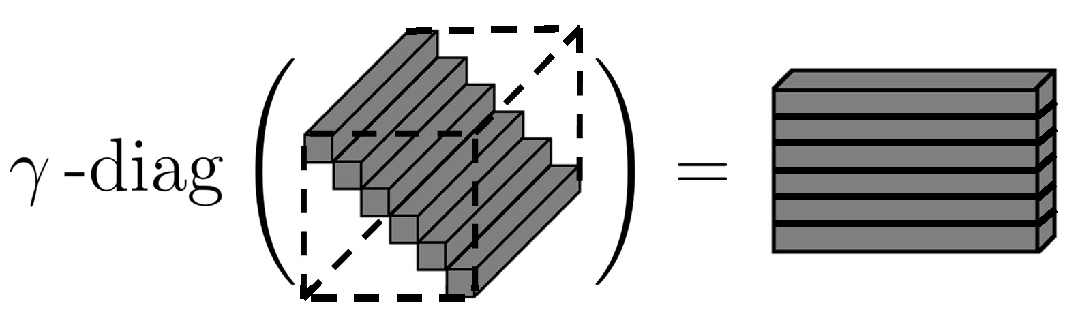
\includegraphics[width=.75\linewidth]{figures/diag3.pdf}
	%   \captionsetup{labelsep=period,justification=justified,singlelinecheck=false}
	%   \caption{$\mydiag$的一个形象展示}
	%   \label{fig:diag3}
	% \end{figure}
\end{definition}

\noindent 对于定义在$\mathbb{R}^{j\times j\times k}$中的三阶张量$\mathbfcal{Y}$,$\mydiag(\mathbfcal{Y}) \in \mathbb{R}^{j\times k}$即代表$\mathbfcal{Y}$的“对角”元素,其行向量由$\mathbfcal{Y}$的前两个索引相同的mode-$3$纤维(即$\{\boldsymbol{y}_{ii:}\}_{i=1}^{j}$)组成。\reffig{fig:diag3}形象地展示了$\mydiag(\cdot)$的作用。

\begin{figure}[!ht]
	  \centering
	  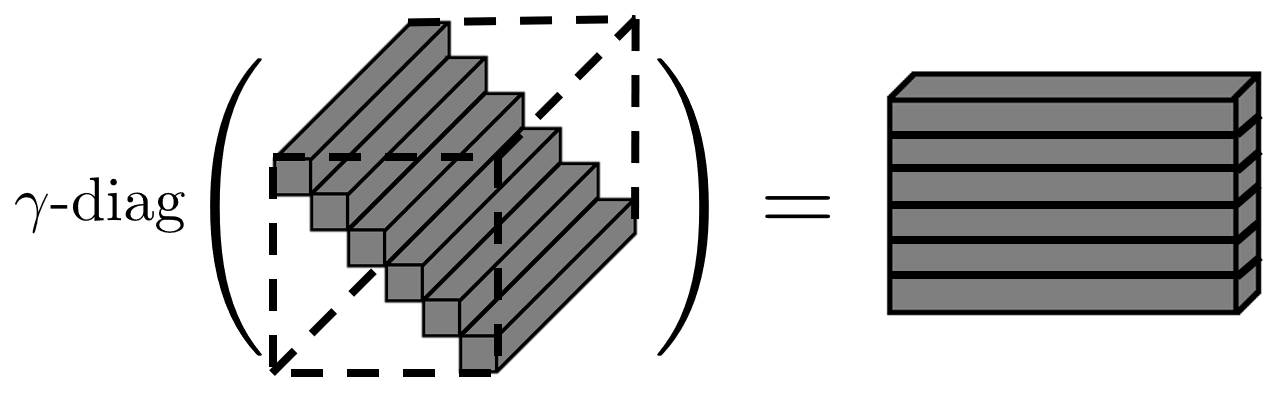
\includegraphics[width=.7\linewidth]{figures/gammadiag.png}
	  \caption{$\mydiag(\cdot)$的示意图}
	  \label{fig:diag3}
\end{figure}

\begin{table}[!t]
% \captionsetup{labelsep=newline}
\centering
\caption{张量相关的符号总结}
\label{tab:tensor-notations}
\begin{tabular}{l|l|l|l}
\hline $\mathbfcal{X}$ & 张量 &  $\boldsymbol{X}_{(i)}$ & $\mathbfcal{X}$的mode-$i$矩阵化\\
$\norm{\mathbfcal{X}}_F$ & $\mathbfcal{X}$的Frobenius范数 & $\boldsymbol{X}_{::i}$或$\boldsymbol{X}^{(i)}$ &
$\mathbfcal{X}$的第$i$个前向切片\\ $\boldsymbol{x}_{ij:}$ & $\mathbfcal{X}$的第$(i,j)$个mode-$3$纤维 & $\mydiag(\mathbfcal{X})$ & $\mathbfcal{X}$的“对角”元素 \\\hline
\end{tabular}
% \vspace{-2em}
\end{table}

% 对一个三维张量$\mathbfcal{X}\in\mathbb{R}^{n_1\times n_2\times n_3}$而言,给定$i=1$,$2$或$3$,则沿着第$i$个mode所对应的方向的那些向量就称为$\mathbfcal{X}$的mode-$i$纤维。我们用$\boldsymbol{X}_{(i)}$来代表张量$\mathbfcal{X}$沿着第$i$个mode的矩阵化(其列向量由张量$\mathbfcal{X}$的mode-$i$纤维按顺序排列而成)。我们用$\mathbfcal{X} \times_{i} \boldsymbol{U}$来代表张量$\mathbfcal{X}$与矩阵$\boldsymbol{U}$ 的mode-$i$积。与矩阵类似,我们用$\norm{\mathbfcal{X}}_{F}$来表示张量$\mathbfcal{X}$的Frobenius范数。此外,我们交替地使用$\boldsymbol{X}_{::i}$或$\boldsymbol{X}^{(i)}$(视实际情况而定)来代表张量$\mathbfcal{X}$的第$i$个前向切片,而用$\boldsymbol{x}_{ij:}$来代表张量$\mathbfcal{X}$的第$(i,j)$个mode-$3$纤维。对于更高维张量,上述符号有类似的拓展,故我们略去介绍。

% 对以下所有操作,我们使用一个$8\times 8\times 8$的张量$\mathbfcal{X}_{\text{示范}}$来作示范。该张量如\reffig{fig:tensorEbyE}所示。

% \subsection{张量纤维}
% \esubsection{The Fibers of Tensors}
% 我们首先介绍张量纤维的概念。张量的纤维是矩阵的行向量与列向量在张量情形下的拓展\ucite{kolda2009tensor}。张量纤维的形式化定义如下。
% \begin{definition}[张量纤维]\kaishu
% 	对一个$d$维张量$\mathbfcal{Y}\in\mathbb{R}^{r_{1}\times r_{2}\times\ldots\times r_{d}}$而言,它的一个mode-$i$纤维由固定所有除第$i$个索引以外的索引得到。
% \end{definition}

% 显然,mode-$i$纤维一共有$\prod_{j=1,j\neq i}^{d}r_{j}$个。

% \reffig{fig:tensor-fibers}展示了三维张量$\mathbfcal{X}_{\text{示范}}$的mode-$1$纤维,mode-$2$纤维以及mode-$3$纤维。

% \begin{figure}[!ht]
% \centering
% \begin{tikzpicture}
% 	% Rows
% 	\foreach \x in {0,0.35,...,2.8}
%     	\foreach \y in {0,0.35,...,2.8}
% 			\tikzcuboidset{hidden edges/.style={dashed}}
% 			\pic[thick,black] (cuboid) at (4,\y,-2.45+\x) {cuboid=3--0.25--0.25};
% 	% Columns
% 	\foreach \x in {0,0.35,...,2.8}
%     	\foreach \y in {0,0.35,...,2.8} 
% 			\tikzcuboidset{hidden edges/.style={dashed}}
% 			\pic[thick,black] (cuboid) at (9+\y,0,-2.45+\x) {cuboid=0.25--3--0.25};

% 	% Mode-3 fibers.
% 	\foreach \x in {0,0.35,...,2.8}
%     	\foreach \y in {0,0.35,...,2.8} 
% 			\tikzcuboidset{hidden edges/.style={dashed}}
% 			\pic[thick,black] (cuboid) at (14+\x,\y,0) {cuboid=0.25--0.25--3};
% \end{tikzpicture}
% \caption{张量$\mathbfcal{X}_{\text{示范}}$的mode-$1$纤维,mode-$2$纤维以及mode-$3$纤维}
% \label{fig:tensor-fibers}
% \end{figure}

% \begin{tikzpicture}
	% \pic[ultra thick,red] at (0,0,0) {cuboid=2--2--2};

	% \tikzcuboidset{hidden edges/.style={dashed}}
	% \pic[thick,black] (cuboid) at (4,0,0) {cuboid=3--3--3};
	% \fill[red] (cuboid-rear left center) circle (2pt);

% 	\tikzcuboidset*{zangle=225}
% 	\pic[thick,black] at (8,0,0) {cuboid};

% 	\tikzcuboidset{all grids/.style={draw=black,thin,step=.5}}
% 	\pic[thin,black] at (10,0,0) {cuboid};

%    \tikzcuboidset{hidden edges/.style={dashed},front face/.style={fill=red!20},right face/.style={fill=blue!20},top face/.style={fill=green!20}}
% 	\pic at (9,2,0) {cuboid};

%    \tikzcuboidset{hidden edges/.style={dashed,draw=white},all faces/.style={fill=black}, edges/.style={draw=white,thick}}
% 	\pic at (12,1,0) {cuboid=2--1--3};
%  \end{tikzpicture} 

% \subsection{张量切片}
% \esubsection{The Slices of Tensors}
% 与张量的纤维类似,我们可以固定除某两个索引以外的所有索引来得到张量的一系列切片。为了本文的完整性,我们给出张量切片的具体定义如下。

% \begin{definition}[张量切片]\kaishu
% 	对一个$d$维张量$\mathbfcal{Y}\in\mathbb{R}^{r_{1}\times r_{2}\times\ldots\times r_{d}}$而言,它的一个mode-$(i,j)$切片由固定所有除第$i$和$j$个索引以外的所有索引得到。
% \end{definition}

% 同理,mode-$(i,j)$切片一共有$\prod_{k=1,k\neq i,k\neq j}^{d}r_{j}$个。对于一个三维张量而言,我们通常称mode-$(2,3)$切片为侧向切片,mode-$(1,3)$切片为水平切片,而mode-$(1,2)$切片为前向切片。

% \reffig{fig:tensor-fibers}展示了三维张量$\mathbfcal{X}_{\text{示范}}$的侧向切片,水平切片以及前向切片。

% \begin{figure}[!ht]
% \centering	
% \begin{tikzpicture}
% 	% Lateral slices
% 	\foreach \x in {0,0.35,...,2.8}
% 		\tikzcuboidset{hidden edges/.style={dashed}}
% 		\pic[thick,black] (cuboid) at (4+\x,0,0) {cuboid=0.25--3--3};
% 	% Horizontal slices
% 	\foreach \x in {0,0.35,...,2.8}
% 		\tikzcuboidset{hidden edges/.style={dashed}}
% 		\pic[thick,black] (cuboid) at (9,\x,0) {cuboid=3--0.25--3};
% 	% Frontal slices
% 	\foreach \x in {0,0.35,...,2.8}
% 		\tikzcuboidset{hidden edges/.style={dashed}}
% 		\pic[thick,black] (cuboid) at (14,0,-2.45+\x) {cuboid=3--3--0.25};
% \end{tikzpicture}
% \caption{张量$\mathbfcal{X}_{\text{示范}}$的侧向切片,水平切片以及前向切片}
% \label{fig:tensor-slices}
% \end{figure}

% \subsection{张量的mode-$n$矩阵化}
% \esubsection{The Mode-$n$ Matricization of Tensors}
% 为了直观且方便地操作张量,我们有时会将张量进行重组,从而将其矩阵化(这个过程也称为张量展开或展平)。直观上来讲,张量的mode-$n$矩阵化即为将它的mode-$n$纤维作为列向量按照索引大小顺序从左到右排列而形成矩阵。张量的mode-$n$矩阵化的形式化定义如下。
% \begin{definition}[张量的mode-$n$矩阵化]\kaishu
% 	对一个$d$维张量$\mathbfcal{Y}\in\mathbb{R}^{r_{1}\times r_{2}\times\ldots\times r_{d}}$而言,它的mode-$n$矩阵化$\boldsymbol{Y}_{(n)}$与原始张量$\mathbfcal{Y}$中元素的一一对应关系为
% 	\begin{equation*}
% 		\text{$x_{i_{1}i_{2}\ldots i_{d}}$与$\parenth{\boldsymbol{X}_{(n)}}_{i_{n}j}$一一对应,其中$j=1+\sum_{k=1, k \neq n}^{d}\left(i_{k}-1\right) \parenth{\prod_{m=1, m \neq n}^{k-1} r_{m}}$}.
% 	\end{equation*}
% \end{definition}
% \reffig{fig:tensor-mode1mat}形象地展示了张量$\mathbfcal{X}_{\text{示范}}$的mode-$1$矩阵化过程。

% \begin{figure}[!ht]
% 	\centering
% 	\begin{tikzpicture}
% 		\foreach \x in {0,0.35,...,2.8}
% 			\foreach \y in {0,0.35,...,2.8} 
% 				\tikzcuboidset{hidden edges/.style={dashed}}
% 				\pic[thick,black] (cuboid) at (4+\y,0,-2.45+\x) {cuboid=0.25--3--0.25};
% 	\node at (9,2.25,0) {\larger[5]$\rightarrow$};
% 	\foreach \x in {0,0.35,...,2.8}
% 		\tikzcuboidset{hidden edges/.style={dashed}}
% 		\pic[thick,black] (cuboid) at (10+\x,0,-2.45) {cuboid=0.25--3--0.25};
% 	\node at (14,2.25,0) {\larger[5]$\rightarrow$};
% 	\end{tikzpicture}
% 	\caption{张量$\mathbfcal{X}_{\text{示范}}$的mode-$1$矩阵化}
% 	\label{fig:tensor-mode1mat}
% \end{figure}

% \subsection{张量的mode-$n$乘法}
% \esubsection{The Mode-$n$ Product of Tensors}
% 张量还可以与一个适当的矩阵(或张量\footnote{张量也可以与张量做乘法,例如张量之间的收缩积\ucite{bader2006algorithm}。但由于这些操作与本文关系不是特别密切,我们便不再详细叙述。})做乘法。我们接下来介绍张量与矩阵的mode-$n$乘法。张量mode-$n$乘法的形式化定义如下。
% \begin{definition}[张量的mode-$n$乘法]\kaishu
% 	对一个$d$维张量$\mathbfcal{Y}\in\mathbb{R}^{r_{1}\times r_{2}\times\ldots\times r_{d}}$而言,它与矩阵$\boldsymbol{U}\in\mathbb{R}^{m\times r_{n}}$的mode-$n$乘法$\mathbfcal{Y}\times_{n}\boldsymbol{U}$构成了一个$r_{1}\times\ldots\times r_{n-1}\times m\times r_{n+1}\times \ldots\times r_{d}$的矩阵,其中
% 	\begin{equation*}
% 		\left(\mathbfcal{Y} \times_{n} \boldsymbol{U}\right)_{i_{1} \ldots i_{n-1} j i_{n+1} \ldots i_{d}}=\sum_{i_{n}=1}^{r_{n}} y_{i_{1} i_{2} \ldots i_{N}} u_{j i_{n}}.
% 	\end{equation*}
% 	此外,我们也可以用之前介绍的mode-$n$展开来表述mode-$n$乘法,即
% 	\begin{equation*}
% 		\mathbfcal{Z}=\mathbfcal{Y} \times_{n} \boldsymbol{U} \iff \boldsymbol{Z}_{(n)}=\boldsymbol{U} \boldsymbol{Y}_{(n)}.
% 	\end{equation*}
% \end{definition}

% \reffig{fig:tensor-modeprod}形象地展示了张量$\mathbfcal{X}_{\text{示范}}$与某一向量的mode-$1$乘法。
% \begin{figure}[!ht]
% \centering
% \begin{tikzpicture}
% 	\tikzcuboidset{all grids/.style={draw=black,thin,step=0.375}}
% 		\pic[thin,black] at (4,0,0) {cuboid=3--3--3};

% 	\node at (9,2.25,0) {\larger[5]$\times_{1}$};

% 	\tikzcuboidset{hidden edges/.style={dashed}}
% 		\pic[thick,black] (cuboid) at (10,0.75,0) {cuboid=0.25--3--0.25};
% 	\node at (11.5,2.25,0) {\larger[5]$=$};
% 	\foreach \x in {0,0.35,...,2.8}
% 		\foreach \y in {0,0.35,...,2.8}
% 			\tikzcuboidset{hidden edges/.style={dashed}}
% 			\pic[thick,black] (cuboid) at (12+\x,1.5,-2.45+\y) {cuboid=0.25--0.25--0.25};
% \end{tikzpicture}
% \caption{张量$\mathbfcal{X}_{\text{示范}}$与某一向量的mode-$1$乘法}
% \label{fig:tensor-modeprod}
% \end{figure}

% \subsection{三维张量“对角”元素}
% \esubsection{The ``Diagonal'' Entries of Three-Dimensional Tensors }

% \subsection{其它杂项}
% \esubsection{Miscellaneous}
本节接下来介绍一些其它符号。
对于随机变量$x$,$\mathbb{E}(x)$代表它的期望,而$\mathbb{V}(x)$代表它的方差。给定概率空间$(\Omega,\mathcal{F},\mathbb{P})$,那么定义$d$维向量序列$\{\boldsymbol{x}_{k}\}\subseteq\mathbb{R}^{d}$依概率收敛到常向量$\boldsymbol{c}\in\mathbb{R}^{d}$,如果$\forall~\epsilon >0$,都有$\lim_{k\rightarrow+\infty}\allowbreak\mathbb{P}(\norm{\boldsymbol{x}_{k}-\boldsymbol{c}}>\epsilon)=0$,其中$\norm{\cdot}$可以为任何范数
% \footnote{这是因为在有限维向量空间中所有范数都是等价的\ucite{trefethen1997numerical},因而它们诱导出的拓扑结构也都是相同的。}
,简记作$\boldsymbol{x}_{k}\rightarrow_{\mathbb{P}}\boldsymbol{c}$。本文视上下文既使用$\circ$代表两个向量之间的外积,也使用$\circ$代表两个函数之间的复合。
% \begin{equation*}
%     \delta(x,y)=
%     \begin{cases}
%       1, & ~\text{若}~x=y, \\
%       0, & ~\text{其它}.
%     \end{cases}
% \end{equation*}
定义$[n]:=\{1,2,\ldots,n\}$。本文视情况交替地使用$i\in[n]$、$i\in\{1,2,\ldots,n\}$以及$i=1,2,\ldots,n$,它们都代表同样的意思。
% 对一个矩阵$\boldsymbol{A}\in\mathbb{R}^{m\times n}$而言,我们简单地使用$\boldsymbol{A} \ge 0$来代表$\boldsymbol{A}\succeq_{\mathbb{R}_{+}^{m\times n}}\{0\}^{m\times n}\iff\boldsymbol{A}-\{0\}^{m\times n}\in\mathbb{R}_{+}^{m\times n}$,意味着$\boldsymbol{A}$的每一个元素被约束至非负。对于一族矩阵$\{\boldsymbol{A}_{i}\}_{i\in\mathcal{I}}$,我们同样简单地使用$\{\boldsymbol{A}_{i}\}_{i\in\mathcal{I}}\geq 0$来代表$\forall~ i\in\mathcal{I}$,$\boldsymbol{A}_{i}$的每一个元素被约束至非负。对于张量,我们有同样的约定,便不再赘述。
$\mathbbm{1}(S)$代表逻辑断言$S$的指示函数,即若$S$为真,则$\mathbbm{1}(S)=1$,否则$\mathbbm{1}(S)=0$。定义Kronecker delta函数为$\delta(x,y):=\mathbbm{1}(x=y)$。

% 为了方便起见,我们在\reftab{tab:notations}我们总结了本文中常用的符号。

% \begin{table}[!t]
% \centering
% \caption{常用符号总结}
% \label{tab:notations}
% \resizebox{\textwidth}{!}{
% \begin{tabular}{l|l|l|l}
% \hline $x$ & A scalar & $\boldsymbol{X}$ & A matrix \\
% $\boldsymbol{x}$ & A vector & $\mathbfcal{X}$ & A tensor \\
% \hline $\boldsymbol{X}^{\top}$ & The transpose of $\boldsymbol{X}$ & $\operatorname{Tr}\left(\boldsymbol{X}\right)$ & $\operatorname{Tr}\left(\boldsymbol{X}\right) = \sum_{i}x_{ii}$ \\ $\|\boldsymbol{X}\|_{F}$ & $\|\boldsymbol{X}\|_{F}=\sqrt{\sum_{i j} x_{i j}^{2}}$ & $\|\boldsymbol{X}\|_{2,1}$ & $\|\boldsymbol{X}\|_{2,1}=\sum_{i}\sqrt{\sum_{j} x_{i j}^{2}}$ \\ \hline $\boldsymbol{X}_{::i}$ & The $i$-th frontal slice of $\mathbfcal{X} $ &  $\|\mathbfcal{X}\|_{F}$ & $\|\mathbfcal{X}\|_{F}=\sqrt{\sum_{i j k}x_{i j k}^{2}}$ \\
% $\boldsymbol{X}^{(i)}$ & $\boldsymbol{X}^{(i)}=\boldsymbol{X}_{::i}$ & $\boldsymbol{X}_{(i)}$ & The mode-$i$ matricization of $\mathbfcal{X} $ \\ $\mathbfcal{X}\times_{i}\boldsymbol{U}$ & The mode-$i$ product of $\mathbfcal{X}$ and $\boldsymbol{U}$ & & \\ \hline $\otimes$ & The Kronecker prduct & $\odot$ & The Khatri-Rao product \\ $\oast$ & The Hadamard product & & \\ \hline
% \end{tabular}
% }
% \end{table}

% \section{张量相关的符号与操作——详细版}
% \esection{Notations and Manipulations Related to Tensors---Detailed Version}
% \begin{wrapfigure}{R}{0.45\linewidth}
% 	\centering
% 	\begin{tikzpicture}
% 			\tikzcuboidset{all grids/.style={draw=black,thin,step=0.375}}
% 			\pic[thin,black] at (10,0,0) {cuboid=3--3--3};
% 	\end{tikzpicture}
% 	\caption{三维示范张量$\mathbfcal{X}_{\text{示范}}\in\mathbb{R}^{8\times8 \times 8}$}
% 	\label{fig:tensorEbyE}
% \end{wrapfigure}	

\section{预备知识}
\esection{Preliminaries}
本节介绍一些重要的预备知识。这些预备知识将为本文提出方法的优化模型建立与优化算法设计作为准备。

\subsection{非负矩阵分解}\label{sec:nmf-dec}
\esubsection{Nonnegative Matrix Factorization}
本节介绍非负矩阵分解以及用于优化非负矩阵分解的Lee-Seung算法\ucite{lee2001algorithms}。给定矩阵$\boldsymbol{V}\in\mathbb{R}_{+}^{n\times m}$,非负矩阵分解即如下数学优化问题
\begin{equation*}
    \begin{aligned}
    & \underset{\smash[b]{\substack{\boldsymbol{W},\boldsymbol{H}}}}{\min}
    & &  \norm{\boldsymbol{V}-\boldsymbol{W}\boldsymbol{H}}_{F}^{2}\\
    & \text{s.t.}
    & & \boldsymbol{W}\in\mathbb{R}_{+}^{n\times r},~\boldsymbol{H}\in\mathbb{R}_{+}^{r\times m}.
    \end{aligned}
\end{equation*}
用于优化非负矩阵分解的经典Lee-Seung算法\ucite{lee2001algorithms}即反复用如下乘法更新公式迭代更新参数矩阵$\boldsymbol{W}$和$\boldsymbol{H}$
\begin{equation*}
\begin{aligned}
    \boldsymbol{W}\leftarrow\boldsymbol{W}\oast\left(\frac{\boldsymbol{V}\boldsymbol{H}^{\top}}{\boldsymbol{W}\boldsymbol{H}\boldsymbol{H}^{\top}}\right),~\boldsymbol{H}\leftarrow\boldsymbol{H}\oast\left(\frac{\boldsymbol{W}^{\top}\boldsymbol{V}}{\boldsymbol{W}^{\top}\boldsymbol{W}\boldsymbol{H}}\right).
\end{aligned}
\end{equation*}
Lee-Seung算法如\refalg{alg:leeseung}所示。此外,文献\ucite{lee2001algorithms}还给出了如下关于Lee-Seung算法的相关定理。

\begin{lemma}[Lee等人\ucite{lee2001algorithms}]\label{lemma:lee-desc}\kaishu
    基于Lee-Seung算法,非负矩阵分解的目标函数$\|\boldsymbol{V}-\boldsymbol{W}\boldsymbol{H}\|_{F}^{2}$在更新的每一步都会得到下降。
\end{lemma}

% \reflemma{lemma:lee-desc}将在本文进行收敛性分析时被反复使用。
\vspace{-1em}

\begin{algorithm}[t]
\setstretch{1.35}
	\begin{algorithmic}[1]
	\REQUIRE 矩阵$\boldsymbol{V}\in\mathbb{R}_{+}^{n\times m}$以及最大迭代步数$\Phi$
	\ENSURE 优化完毕后的参数矩阵
	\STATE 赋$t\leftarrow 0$,并随机初始化$\boldsymbol{W}_{t}\in\mathbb{R}_{+}^{n\times r}$和$\boldsymbol{H}_{t}\in\mathbb{R}_{+}^{r\times m}$;
	\WHILE{$t<\Phi$并且算法未收敛}
    \STATE 更新$\boldsymbol{W}_{t+1}\leftarrow\boldsymbol{W}_{t}\oast(({\boldsymbol{V}\boldsymbol{H}_{t}^{\top}})\oslash({\boldsymbol{W}_{t}\boldsymbol{H}_{t}\boldsymbol{H}_{t}^{\top}}))$;
    \STATE 更新$\boldsymbol{H}_{t+1}\leftarrow\boldsymbol{H}_{t}\oast(({\boldsymbol{W}_{t+1}^{\top}\boldsymbol{V}})\oslash({\boldsymbol{W}_{t+1}^{\top}\boldsymbol{W}_{t+1}\boldsymbol{H}_{t}}))$;
	\STATE 赋$t\leftarrow t+1$;
	\ENDWHILE
	\RETURN $\boldsymbol{W}_{t}$以及$\boldsymbol{H}_{t}$;
	\end{algorithmic}
	\captionsetup{labelsep=period,font=bf}
	\caption{Lee-Seung算法\ucite{lee2001algorithms}}
	\label{alg:leeseung}
\end{algorithm}

\subsection{(非负)张量CP分解与Tucker分解}\label{sec:tensor-decomp}
\esubsection{(Nonnegative) Tensor CP and Tucker Decompositions}
本节介绍(非负)张量CP分解与Tucker分解。这两个张量分解技术是本文提出的所有方法的基石。

张量CP分解是张量聚类分析的常用手段\ucite{huang2008simultaneous}。张量CP分解旨在将张量分解成若干个秩-$1$张量之和。具体而言,给定张量样本$\mathbfcal{X}^{(0)}\in \mathbb{R}^{n_1 \times n_2 \times \ldots \times n_d}$以及所期待的张量CP分解的秩$r_{0}\in\mathbb{N}\setminus\{0\}$,那么$\mathbfcal{X}^{(0)}$的CP分解即为
\begin{equation}\label{eq:cp-approx}
	\mathbfcal{X}^{(0)}\approx\sum_{r=1}^{r_{0}}\boldsymbol{a}^{(1)}_{:r} \circ \boldsymbol{a}^{(2)}_{:r} \circ \ldots \circ \boldsymbol{a}^{(d)}_{:r},
\end{equation}
其中$\boldsymbol{A}^{(j)}\in\mathbb{R}^{n_{j}\times r_{0}}$为CP分解的mode-$j$参数矩阵($j=1,2,\ldots,d$)。此外,本文使用文献\ucite{kolda2006multilinear}中介绍的符号$\llbracket \boldsymbol{A}^{(1)}, \boldsymbol{A}^{(2)}, \ldots, \boldsymbol{A}^{(d)} \rrbracket$来代替$\sum_{r=1}^{r_{0}}\boldsymbol{a}^{(1)}_{:r} \circ \boldsymbol{a}^{(2)}_{:r} \circ \ldots \circ \boldsymbol{a}^{(d)}_{:r}$。除此之外,也可以将\refequation{eq:cp-approx}用mode-$k$展开等价地写为
\begin{equation*}
	\begin{aligned}
		\boldsymbol{X}^{(0)}_{(k)} \approx  \boldsymbol{A}^{(k)}\left(\boldsymbol{A}^{(d)} \odot \ldots \odot \boldsymbol{A}^{(k+1)} \odot \boldsymbol{A}^{(k-1)} \odot \ldots \odot \boldsymbol{A}^{(1)} \right)^{\top}.
		\end{aligned}
\end{equation*}
这个公式在将张量问题转换为矩阵问题时非常有用。人们通常使用张量Frobenius范数诱导的度量来构建如下优化模型
\begin{equation*}\label{cp}
	\begin{aligned}
		&\underset{\{\boldsymbol{A}^{(j)}\}_{j=1}^{d}}{\min}&& \left\|\mathbfcal{X}^{(0)}-\llbracket \boldsymbol{A}^{(1)}, \boldsymbol{A}^{(2)}, \ldots, \boldsymbol{A}^{(d)} \rrbracket\right\|_{F},
	\end{aligned}
\end{equation*}
并通过求解该模型来数值计算张量CP分解。
% \reffig{fig:tensor-cp}展示了三维示范张量$\mathbfcal{X}_{\text{示范}}$由CP分解分解为一系列秩-$1$的张量的过程。
% \begin{figure}[!ht]
% 	\centering
% 	\begin{tikzpicture}
% 		\tikzcuboidset{hidden edges/.style={dashed}}
% 			\pic[thin,black] at (4,0,0) {cuboid=3--3--3};
% 		\node at (9,2.25,0) {\larger[5]$\approx$};
% 		\node at (11,1.5,0) {\larger[5]$\boldsymbol{a}_{:1}$};
% 		\node at (12.5,4,0) {\larger[5]$\boldsymbol{b}_{:1}$};
% 		\node at (10.25,4.25,0) {\larger[5]$\boldsymbol{c}_{:1}$};
% 		\tikzcuboidset{hidden edges/.style={dashed}}
% 			\pic[thin,black] at (10,0,0) {cuboid=0.25--3--0.25};
% 		\tikzcuboidset{hidden edges/.style={dashed}}
% 			\pic[thin,black] at (10,3.25,0) {cuboid=0.25--0.25--3};
% 		\tikzcuboidset{hidden edges/.style={dashed}}
% 			\pic[thin,black] at (10.4,3,0) {cuboid=3--0.25--0.25};
% 		\node at (15,2.25,0) {\larger[5]$+\ldots+$};
% 		\node at (17.5,1.5,0) {\larger[5]$\boldsymbol{a}_{:R}$};
% 		\node at (19,4,0) {\larger[5]$\boldsymbol{b}_{:R}$};
% 		\node at (16.75,4.25,0) {\larger[5]$\boldsymbol{c}_{:R}$};
% 		\tikzcuboidset{hidden edges/.style={dashed}}
% 			\pic[thin,black] at (16.5,0,0) {cuboid=0.25--3--0.25};
% 		\tikzcuboidset{hidden edges/.style={dashed}}
% 			\pic[thin,black] at (16.5,3.25,0) {cuboid=0.25--0.25--3};
% 		\tikzcuboidset{hidden edges/.style={dashed}}
% 			\pic[thin,black] at (16.9,3,0) {cuboid=3--0.25--0.25};
% 		\node at (6,2,0) {\larger[5]$\mathbfcal{X}_{\text{示范}}$};
% 	\end{tikzpicture}
% 	\caption{张量CP分解:$\mathbfcal{X}_{\text{示范}}\approx\llbracket\boldsymbol{A},\boldsymbol{B},\boldsymbol{C}\rrbracket$}
% 	\label{fig:tensor-cp}
% \end{figure}
此外,由于数据有时是非负的,因而为了结合数据的非负属性以提升模型的性能及可解释性,人们往往还会对张量CP分解施加非负约束,即非负张量CP分解。具体而言,非负张量CP分解的优化模型为
\begin{equation*}\label{cp-nn}
	\begin{aligned}
		&\underset{\mathclap{\{\boldsymbol{A}^{(j)}\}_{j=1}^{d}}}{\min}\quad&& \left\|\mathbfcal{X}^{(0)}-\llbracket \boldsymbol{A}^{(1)}, \boldsymbol{A}^{(2)}, \ldots, \boldsymbol{A}^{(d)} \rrbracket\right\|_{F} \\
		&\text{s.t.} &&\boldsymbol{A}^{(j)}\in \mathbb{R}_{+}^{n_j \times r_{0}},~\forall~j\in[d],
	\end{aligned}
\end{equation*}
其中各符号的意义与普通的张量CP分解一致。

张量Tucker分解\ucite{kolda2009tensor,kolda2006multilinear}(尤其是下面将提到的非负张量Tucker分解)是用于张量特征提取的常用模型。具体而言,给定张量样本$\mathbfcal{X}^{(0)}\in \mathbb{R}^{n_1 \times n_2 \times \ldots \times n_d}$以及核心张量的维度$r_1, r_2, \ldots, r_d$,那么$\mathbfcal{X}^{(0)}$的张量Tucker分解即为
\begin{equation}\label{eq:tucker-approx}
	\mathbfcal{X}^{(0)}\approx\mathbfcal{G}^{(0)} \times_{1} \boldsymbol{A}^{(1)} \times_{2} \boldsymbol{A}^{(2)} \times_{3} \ldots \times_{d} \boldsymbol{A}^{(d)},
\end{equation}
其中$\mathbfcal{G}^{(0)} \in \mathbb{R}^{r_1 \times r_2 \times \ldots \times r_d}$为Tucker分解的核心张量,而$\boldsymbol{A}^{(j)}\in\mathbb{R}^{n_{j}\times r_{j}}$为Tucker分解的mode-$j$参数矩阵($j=1,2,\ldots,d$)。
% 此外,我们常用文献\ucite{kolda2006multilinear}中介绍的符号$\llbracket \mathbfcal{G}^{(0)}; \boldsymbol{A}^{(1)}, \boldsymbol{A}^{(2)},\allowbreak \ldots,\allowbreak \boldsymbol{A}^{(d)} \rrbracket$来代替$\mathbfcal{G}^{(0)} \times_{1} \boldsymbol{A}^{(1)} \times_{2} \boldsymbol{A}^{(2)} \ldots \times_{d} \boldsymbol{A}^{(d)}$。
除此之外,还可以将\refequation{eq:tucker-approx}用mode-$k$展开等价地写为
\begin{equation*}
		\boldsymbol{X}^{(0)}_{(k)} \approx \boldsymbol{A}^{(k)} \boldsymbol{G}^{(0)}_{(k)}\left(\boldsymbol{A}^{(d)} \otimes \ldots \otimes \boldsymbol{A}^{(k+1)} \otimes \boldsymbol{A}^{(k-1)} \otimes \ldots \boldsymbol{A}^{(1)}\right)^{\top}.
\end{equation*}
% 这个公式将会在我们将一个张量问题转换为矩阵问题时非常有用。
人们通常使用张量Frobenius范数诱导的度量来构建如下优化模型
\begin{equation*}\label{tk}
	\begin{aligned}
		&\underset{\mathbfcal{G}^{(0)},~\{\boldsymbol{A}^{(j)}\}_{j=1}^{d}}{\min}&& {\left\|\mathbfcal{X}^{(0)}-\mathbfcal{G}^{(0)} \times_{1} \boldsymbol{A}^{(1)} \times_{2} \boldsymbol{A}^{(2)} \times_{3} \ldots \times_{d} \boldsymbol{A}^{(d)} \right\|_{F}},
	\end{aligned}
\end{equation*}
并通过求解该模型来数值计算张量Tucker分解。
% \reffig{fig:tensor-tucker}展示了三维示范张量$\mathbfcal{X}_{\text{示范}}$由Tucker分解分解为一个核心张量$\mathbfcal{G}$以及三个参数矩阵$\boldsymbol{A}$,$\boldsymbol{B}$,$\boldsymbol{C}$的过程。
% \begin{figure}[!ht]
% \centering
% \begin{tikzpicture}
% 	\tikzcuboidset{hidden edges/.style={dashed}}
% 		\pic[thin,black] at (4,0,0) {cuboid=3--3--3};
% 	\node at (9,2.25,0) {\larger[5]$\approx$};
% 	\tikzcuboidset{hidden edges/.style={dashed}}
% 		\pic[thin,black] at (9,0,-2) {cuboid=1.5--3--0};
% 	\tikzcuboidset{hidden edges/.style={dashed}}
% 		\pic[thin,black] at (10,0,-4) {cuboid=1.5--1.5--1.5};
% 	\tikzcuboidset{hidden edges/.style={dashed}}
% 		\pic[thin,black] at (8.5,0,-10) {cuboid=1.5--0--3};
% 	\tikzcuboidset{hidden edges/.style={dashed}}
% 		\pic[thin,black] at (12,0,-5) {cuboid=3--1.5--0};
% 	\node at (6,2,0) {\larger[5]$\mathbfcal{X}_{\text{示范}}$};
% 	\node at (10.5,2.25,0) {\larger[5]$\boldsymbol{A}$};
% 	\node at (13.75,4.2,0) {\larger[5]$\boldsymbol{B}$};
% 	\node at (15.5,2.75,0) {\larger[5]$\boldsymbol{C}$};
% 	\node at (12.5,2.5,0) {\larger[5]$\mathbfcal{G}$};
% \end{tikzpicture}
% \caption{张量Tucker分解:$\mathbfcal{X}_{\text{示范}}\approx\llbracket\mathbfcal{G};\boldsymbol{A},\boldsymbol{B},\boldsymbol{C}\rrbracket$}
% \label{fig:tensor-tucker}
% \end{figure}
% 由于数据有时是非负的,因而为了结合数据的非负属性以提升模型的性能及可解释性,我们往往还会对Tucker分解施加非负约束,即非负张量Tucker分解。具体而言,
此外,非负张量Tucker分解的优化模型为
\begin{equation*}\label{tk-nn}
	\begin{aligned}
		&\underset{\mathclap{\mathbfcal{G}^{(0)},~\{\boldsymbol{A}^{(j)}\}_{j=1}^{d}}}{\min}\qquad&& {\left\|\mathbfcal{X}^{(0)}-\mathbfcal{G}^{(0)} \times_{1} \boldsymbol{A}^{(1)} \times_{2} \boldsymbol{A}^{(2)} \times_{3} \ldots \times_{d} \boldsymbol{A}^{(d)} \right\|_{F}} \\
		&\text{s.t.} &&\mathbfcal{G}^{(0)}\in\mathbb{R}_{+}^{r_1 \times r_2 \times \ldots \times r_d},~\boldsymbol{A}^{(j)}\in \mathbb{R}_{+}^{n_j \times r_j},~\forall~j\in[d],
	\end{aligned}
\end{equation*}
其中各符号的意义与普通的张量Tucker分解一致。

对于(非负)张量CP/Tucker分解的优化算法,本文推荐读者参考文献\ucite{kolda2009tensor,nnegTucker}。

% 此外,由于张量Frobenius范数对噪声与离群点抑制能力较差,文献中另一种常见的非负张量Tucker分解为如下的基于张量$\ell_{1}$范数的非负张量Tucker分解
% \begin{equation*}\label{tk-nn-l1}
% 	\begin{array}{ll}
% 		\min\limits_{\mathbfcal{G}^{(0)}, \boldsymbol{A}^{(j)}} & {\left\|\mathbfcal{X}^{(0)}-\mathbfcal{G}^{(0)} \times_{1} \boldsymbol{A}^{(1)} \times_{2} \boldsymbol{A}^{(2)} \ldots \times_{d} \boldsymbol{A}^{(d)} \right\|_{1}} \\
% 		\text{~~s.t.} &\mathbfcal{G}^{(0)} \ge 0,\, \{\boldsymbol{A}^{(j)}\}_{j=1}^{d}\ge 0.
% 	\end{array}
% \end{equation*}

\subsection{基于张量优化的无监督特征提取的$\ell_{2}$方法}\label{sec:l2}
\esubsection{The $\ell_{2}$ Method for Tensor Optimization-Based Unsupervised Feature Extraction}
% \subsection{$\ell_{2}$方法}\label{sec:l2}
% \esubsection{The $\ell_{2}$ Method}
本节介绍无监督特征提取中的基于$\ell_{2}$范数的非负张量Tucker分解方法(简称$\ell_{2}$方法)。这个方法可以看作是\refsection{sec:review-ufe}中所综述的大部分非鲁棒方法的核心。考虑由$n$个张量样本$\mathbfcal{X}^{(i)}$($i=1,2,\ldots,n$)垛叠而成的张量$\mathbfcal{X} \in \mathbb{R}_{+}^{n_1 \times n_2 \times \ldots \times n_d \times n}$(关于无监督特征提取任务中的数据形式约定,请参考\refsection{sec:dataasump}),则用于从$\mathbfcal{X}$提取特征的$\ell_{2}$方法的优化模型为
\begin{equation}\label{eq:L2}
\hspace{1em}
    \begin{aligned}
    &\underset{\mathclap{\{\mathbfcal{G}^{(i)}\}_{i=1}^{n}, \{\boldsymbol{A}^{(j)}\}_{j=1}^{d}}}{\min} \qquad\quad &&\sum_{i=1}^{n}\left\|\mathbfcal{X}^{(i)}-\mathbfcal{G}^{(i)} \times_{1} \boldsymbol{A}^{(1)} \times_{2} \boldsymbol{A}^{(2)} \times_{3} \ldots \times_{d} \boldsymbol{A}^{(d)}\right\|_{F}^{2} \\
    &\text{s.t.} && \mathbfcal{G}^{(i)}\in\mathbb{R}_{+}^{r_1 \times r_2 \times \ldots \times r_d},~\forall~i\in[n] ,~\boldsymbol{A}^{(j)}\in \mathbb{R}_{+}^{n_j \times r_j},~\forall~j\in[d],
    \end{aligned}
\end{equation}
其中$\mathbfcal{G}^{(i)}$被视作从$\mathbfcal{X}^{(i)}$提取的特征,而$\boldsymbol{A}^{(j)}$($j=1,2,\ldots, d$)则被视为共享于所有数据样本之间的特征提取器。如果记$\epsilon_{i}=\|\mathbfcal{X}^{(i)}-\mathbfcal{G}^{(i)} \times_{1} \boldsymbol{A}^{(1)} \times_{2} \boldsymbol{A}^{(2)} \times_{3} \ldots \times_{d} \boldsymbol{A}^{(d)}\|_{F}$,
% \begin{equation*}
%     \begin{bmatrix}
%         \left\|\mathbfcal{X}^{(1)}-\mathbfcal{G}^{(1)} \times_{1} \boldsymbol{A}^{(1)} \times_{2} \boldsymbol{A}^{(2)} \times_{3} \ldots \times_{d} \boldsymbol{A}^{(d)}\right\|_{F} \\
%         \left\|\mathbfcal{X}^{(2)}-\mathbfcal{G}^{(2)} \times_{1} \boldsymbol{A}^{(1)} \times_{2} \boldsymbol{A}^{(2)} \times_{3} \ldots \times_{d} \boldsymbol{A}^{(d)}\right\|_{F} \\
%         \vdots \\
%         \left\|\mathbfcal{X}^{(n)}-\mathbfcal{G}^{(n)} \times_{1} \boldsymbol{A}^{(1)} \times_{2} \boldsymbol{A}^{(2)} \times_{3} \ldots \times_{d} \boldsymbol{A}^{(d)}\right\|_{F}
%     \end{bmatrix}\in\mathbb{R}^{n},
% \end{equation*}
则$\ell_{2}$方法的目标函数等于向量$\bm{\epsilon}=[\epsilon_1,\epsilon_2,\ldots,\epsilon_n]^{\top}\in\mathbb{R}^{n}$的$\ell_{2}$范数的平方。这便是$\ell_{2}$方法的名称意义所在。
% 可以直接应用文献\ucite{nnegTucker}中介绍的算法优化$\ell_{2}$方法。

$\ell_{2}$方法的原理是优化所有样本的Tucker分解拟合误差的平方总和。这样做的好处是优化难度并不会很高,因为目标函数是光滑的。然而,在现实应用场景中,观察到的数据通常是不确定的。例如,信号通常不能被精确地测量,并且同一信号在不同的测量试验时测得的值通常会波动。虽然数据的波动通常很小,但棘手的问题是,哪怕是数据的略微变化也可以大大影响相应优化问题的最优解。由机器学习理论\ucite{Goodfellow2016},$\ell_{2}$范数相比于$\ell_{1}$范数等其它范数就处理数据中的噪声与离群点的能力而言并不够强,因此使用$\ell_{2}$方法在噪声环境下进行特征提取并不够鲁棒。此外,$\ell_{2}$方法分配给不同样本的权重是相同的,但这并不是合理的。直观上来讲,具有更大拟合误差的样本应该被给予更多的关注。

\subsection{张量Tucker分解的核心张量维度的确定}
\esubsection{Determination of the Dimensionality of the Core Tensor in Tensor Tucker Decomposition}
在对张量$\mathbfcal{X} \in \mathbb{R}_{+}^{n_1 \times n_2 \times \ldots \times n_d \times n}$进行特征提取(Tucker分解)之前,必须为核心张量指定其维度。然而,这并不是简单且随意的问题,因为核心张量的维度大小将会影响特征提取的性能,因而必须通过仔细地分析数据特性以设置。
% 具体来讲,在我们的问题设定下,如果我们事先知道张量$\mathbfcal{X}$是rank-($r_1,r_2, \ldots ,r_d$)的,那么核心张量$\mathcal{G}$应该被定义在空间$\mathbb{R}_{+}^{r_1\times\ldots\times r_d \times n}$中。 然而,实际情况下,我们一般无法事先知道张量$\mathbfcal{X}$的$k$-秩。因此,我们必须对张量$\mathbfcal{X}$进行$k$-秩估计。
本文采用文献\ucite{2010TDFE}中介绍的方法来确定核心张量的维度,
% 我们将被估计的秩值称为张量$\mathbfcal{X}$的本征秩。
具体做法如下:首先,分别对集合$\{\boldsymbol{X}_{(1)}\boldsymbol{X}_{(1)}^{\top},\boldsymbol{X}_{(2)}\boldsymbol{X}_{(2)}^{\top},\ldots,\allowbreak\boldsymbol{X}_{(d)}\boldsymbol{X}_{(d)}^{\top}\}$中的每个矩阵做特征值分解,即$\boldsymbol{X}_{(i)}\boldsymbol{X}_{(i)}^{\top} = \boldsymbol{U}\boldsymbol{\Lambda} \boldsymbol{U}^{\top}\in\mathbb{R}^{n_i \times n_i}$,$\forall~i=1,2,\ldots,d$,其中$\boldsymbol{\Lambda}\in \mathbb{R}_{+}^{n_i \times n_i}$为对角矩阵,其对角线元素包含了矩阵$\boldsymbol{X}_{(i)}\boldsymbol{X}_{(i)}^{\top}$的特征值。然后,将矩阵$\boldsymbol{\Lambda}$的对角线元素从大到小排序,并记排序后的向量为$\boldsymbol{\lambda} \in \mathbb{R}_{+}^{n_i}$。最后,核心张量第$i$维的维度被确定为满足$\sum_{j=1}^{r} \lambda_j/\sum_{j=1}^{n_i} \lambda_j \ge 98\%$的最小的$r$(核心张量最后一维的维度显然应该为$n$,因为一共有$n$个样本,故不需要被确定)。上述算法如\refalg{alg_re}所示。简而言之,$\forall~i=1,2,\ldots,d$,核心张量第$i$维的维度被确定为矩阵$\boldsymbol{X}_{(i)}\boldsymbol{X}_{(i)}^{\top}$的占主导的特征值个数。通过这样的方式所确定的核心张量的维度并不会太大,但其将包含数据中绝大部分的信息,因而该方法是确定核心张量的维度的不错选择。本文在实验中都将使用\refalg{alg_re}来分别为不同数据集确定Tucker分解的核心张量的维度。
此外,本文作者的指导老师陈碧连副教授近年来对该领域有过深入研究,例如提出了自适应核心张量维度的Tucker分解算法\ucite{chen2015optimal}等等。如果读者想了解更多细节,请参考其文章\ucite{chen2015optimal,chen2019nonnegative}。

\begin{algorithm}[t]\setstretch{1.35}
    \begin{algorithmic}[1]
	\REQUIRE 张量$\mathbfcal{X} \in \mathbb{R}^{n_1 \times n_2 \times \ldots \times n_d \times n}$
	\ENSURE 张量$\mathbfcal{X}$的Tucker分解核心张量的维度
	
	\FOR{$i = 1,2,\ldots,d$}
	\STATE 做特征值分解$\boldsymbol{X}_{(i)}\boldsymbol{X}_{(i)}^{\top} = \boldsymbol{U}\boldsymbol{\Lambda} \boldsymbol{U}^{\top}$;
		
	\STATE 将$\operatorname{diag}(\boldsymbol{\Lambda})$中的值从大到小排序,并记排序后的向量为$\boldsymbol{\lambda}$;
		
	\STATE $r_i\leftarrow$满足$\sum_{j=1}^{r} \lambda_j/\sum_{j=1}^{n_i} \lambda_j \geq 98\%$的最小的$r$;
	\ENDFOR
	\RETURN $r_1, r_2,\ldots, r_d, n$;
    \end{algorithmic}
    \captionsetup{labelsep=period,font=bf}
	\caption{核心张量维度确定算法(文献\ucite{2010TDFE})}
	\label{alg_re}
\end{algorithm}

\subsection{图正则}\label{sec:graphreg}
\esubsection{Graph Regularization}
图正则是数据分析中保留数据局部几何结构的有效手段\ucite{cai2010graph}。具体来讲,图正则迫使在数据局部几何结构上相似的样本具有一致的嵌入向量
% (此处的嵌入向量为很宽泛的概念,例如它可以为聚类指示向量,被提取的低维特征等等)
。根据图正则理论\ucite{cai2010graph},数据的局部几何结构可以被带权$k$近邻图有效建模,其中带权$k$近邻图的节点代表不同的数据样本,而其边则代表不同数据样本之间的相似度。具体来讲,给定张量样本$\{\mathbfcal{X}^{(1)},\mathbfcal{X}^{(2)},\ldots,\mathbfcal{X}^{(n)}\}\subseteq\mathbb{R}^{n_{1}\times n_{2}\times \ldots \times n_{d}}$,可以构建邻接矩阵$\boldsymbol{S}$为如下定义的带权$k$近邻图
\begin{equation*}
s_{i j}=\begin{cases}
	\exp\left(\frac{\left\|\mathbfcal{X}^{(i)}-\mathbfcal{X}^{(j)}\right\|_{F}^{2}}{- \sigma^{2}}\right), & ~\text{若}~ \mathbfcal{X}^{(i)} \in \mathcal{N}_{k}\left(\mathbfcal{X}^{(j)}\right)~\text{或}~\mathbfcal{X}^{(j)} \in \mathcal{N}_{k}\left(\mathbfcal{X}^{(i)}\right), \\
	0, & ~\text{其它},
  \end{cases}
\end{equation*}
其中$\mathcal{N}_{k}\left(\mathbfcal{X}^{(i)}\right)$代表样本$\mathbfcal{X}^{(i)}$的$k$近邻集合,而$\sigma$则为高斯核的宽度参数。有了由上述公式定义的带权$k$近邻图,便可以通过最小化以下目标函数来有效地保留数据的局部几何结构\ucite{shi2000normalized, ndfs, cai2010graph}
\begin{equation*}
\begin{aligned}
    &\underset{\mathclap{\boldsymbol{C}}}{\min} && \frac{1}{2} \sum_{i, j=1}^{n} s_{i j}\left\|\frac{\boldsymbol{c}_{:i}}{\sqrt{d_{i i}}}-\frac{\boldsymbol{c}_{:j}}{\sqrt{d_{j j}}}\right\|_{2}^{2}=\operatorname{Tr}\left(\boldsymbol{C}^{\top} \boldsymbol{L C}\right),
\end{aligned}
\end{equation*}
其中$\boldsymbol{C}$代表这些样本的嵌入矩阵,$\boldsymbol{L}=\boldsymbol{I}_{n}-\boldsymbol{D}^{-1/2}\boldsymbol{S}\boldsymbol{D}^{-1/2}$为邻接矩阵$\boldsymbol{S}$的归一化拉普拉斯矩阵,而$\boldsymbol{D}=\operatorname{diag}(\boldsymbol{S}\boldsymbol{1}_{n})$则为邻接矩阵$\boldsymbol{S}$的度矩阵。

% \section{凸分析}
% \esection{Convex Analysis}
% 这一小节简要介绍一些简单的凸分析基础\ucite{fukushima}。这些知识将会对后续的模型分析提供理论支持。
% \begin{definition}[凸集]\kaishu
% 集合$\mathcal{S}$称为凸集,若对任意点$\boldsymbol{x}\in\mathcal{S}$和$\boldsymbol{y}\in\mathcal{S}$,都有$(1-\alpha)\boldsymbol{x}+\alpha\boldsymbol{y}\in\mathcal{S},~\forall~\alpha\in[0,1]$。
% \end{definition}

% 直观上来讲,对于任意属于集合$\mathcal{S}$的两点$\boldsymbol{x}$,$\boldsymbol{y}$,它们的的连线上的所有点都属于$\mathcal{S}$,如图\reffig{fig:convexset}所示。
% \begin{figure}[!ht]
% \centering
% \begin{tikzpicture}
% \begin{axis}[
% 	xmin=-3,   xmax=3,
% 	ymin=-4,   ymax=4,
% 	extra tick style={grid=major},
% ]
% 	\draw[fill=lightgray] \pgfextra{
% 	  \pgfpathellipse{\pgfplotspointaxisxy{0}{0}}
% 		{\pgfplotspointaxisdirectionxy{1.5}{1.5}}
% 		{\pgfplotspointaxisdirectionxy{0}{3}}
% 	};
% 	\node[label=180:$\boldsymbol{x}$,circle,fill,inner sep=2pt] at (axis cs:-0.8,-2.1) {};
% 	\node[label=180:$\boldsymbol{y}$,circle,fill,inner sep=2pt] at (axis cs:0.9,1.8) {};
% 	\draw (axis cs:-0.8,-2.1) -- (axis cs:0.9,1.8);
% % 	\node[label={180:{$\boldsy$}},circle,fill,inner sep=2pt] at (axis cs:-0.8,-2.1) {};
% % 	\addplot [only marks,mark=*] coordinates { (-0.8,-2.1) [$\boldsymbol{x}$] };
% \end{axis}
% \end{tikzpicture}
% \caption{一个简单的凸集}
% \label{fig:convexset}
% \end{figure}

% \begin{definition}[凸函数]\kaishu
% 凸函数有许多等价定义,这里给出一种较为简单的定义。一个实值函数$f:\mathbb{R}^{n}\rightarrow\mathbb{R}$是凸函数,当且仅当它的上图$\epi f\subseteq\mathbb{R}^{n}\times\mathbb{R}$是凸集。
% \end{definition}

% 例如,\reffig{fig:func1}所示函数$f(x)=x^{2}/4$即为一个函数:它的上图明显是凸的。

% \begin{figure}[!ht]
% \centering
% \begin{tikzpicture}
% 	\begin{axis}[
% 		xlabel=$x$,
% 		ylabel={$f(x)=x^{2}/4$}
% 	]
% 	% use TeX as calculator:
% 	\addplot[fill=lightgray,mark=o] {(x^2)/4};
% 	\end{axis}
% \end{tikzpicture}
% \caption{一个简单的凸函数$f(x)=x^{2}/4$}
% \label{fig:func1}
% \end{figure}


% \begin{definition}[锥与凸锥]\kaishu
% 集合$\mathcal{S}$是锥,如果对任意$\boldsymbol{x}\in \mathcal{S}$,均有$k\boldsymbol{x}\in \mathcal{S}$,$\forall~ k\in\mathbb{R}_{++}$。直观上来说,锥中的向量经过任意拉伸缩放之后仍然属于这个锥。如果一个锥同时还是一个凸集,那么我们称之为凸锥。
% \end{definition}

% \reffig{fig:cone}阴影部分展示了一个简单的锥。但很遗憾,它不是凸锥。

% \begin{figure}[!ht]
% \centering
% \begin{tikzpicture}
%     \begin{axis}[thick,smooth,no markers,
% 		xmajorticks=false,
% 		ymajorticks=false,
% 		xmin=-6,
% 		xmax=6,
% 		ymin=-6,
% 		ymax=6]
%         \addplot+[name path=A,black] {0.5*x};
%         \addplot+[name path=B,black] {-0.5*x};
% 		\node[label=270:$\boldsymbol{0}$,circle,fill,inner sep=2pt] at (axis cs:0,0) {};
%         \addplot[lightgray] fill between[of=B and A];
%     \end{axis}
% \end{tikzpicture}
% \caption{一个简单的锥}
% \label{fig:cone}
% \end{figure}

% 通过验证凸集的定义,我们可以判断一个锥是否还是凸锥。但是依据定义来判断在某些情况下会比较繁琐。\reflemma{lemma:convexcone}给出了判断一个锥是否为凸锥的更简单的判断条件。

% \begin{lemma}\label{lemma:convexcone}\kaishu
%     我们有以下等价关系
%     \begin{equation*}
%         \boxed{\text{锥$\mathcal{S}$是凸锥}}\iff\boxed{\boldsymbol{x}\in\mathcal{S}\text{ 且 }\boldsymbol{y}\in\mathcal{S}\implies\boldsymbol{x}+\boldsymbol{y}\in\mathcal{S}}
%     \end{equation*}
% \end{lemma}

% \begin{proof}

% $(\implies)$:由于$\mathcal{S}$是凸集,那么$\forall~ \boldsymbol{x},\boldsymbol{y}\in \mathcal{S}$,我们有$\alpha\boldsymbol{x}+(1-\alpha)\boldsymbol{y}\in \mathcal{S}$。取$\alpha=\frac{1}{2}$,那么我们有$\frac{1}{2}(\boldsymbol{x}+\boldsymbol{y})\in \mathcal{S}$。注意到$\mathcal{S}$是一个锥,我们有$\boldsymbol{x}+\boldsymbol{y}=2\cdot\frac{1}{2}(\boldsymbol{x}+\boldsymbol{y})\in \mathcal{S}$。

% $(\impliedby)$:由于$\mathcal{S}$是一个锥,那么$\forall~ \boldsymbol{x},\boldsymbol{y}\in \mathcal{S}$,我们有$\alpha\boldsymbol{x}\in \mathcal{S}$以及$(1-\alpha)\boldsymbol{y}\in \mathcal{S}$。注意到假设条件$\boldsymbol{x}\in \mathcal{S}\text{~且~}\boldsymbol{y}\in \mathcal{S}\implies\boldsymbol{x}+\boldsymbol{y}\in \mathcal{S}$,从而我们得到$\alpha\boldsymbol{x}+(1-\alpha)\boldsymbol{y}\in \mathcal{S}$. 
% \end{proof}

% \begin{definition}[二阶锥]\kaishu
% 集合$\mathcal{Q}^{n+1}$是$n+1$维空间中的二阶锥,如果$\mathcal{Q}^{n+1}$可以被表示成$\{(\boldsymbol{x},y)\in\mathbb{R}^{n}\times\mathbb{R}_{+}\vert\norm{\boldsymbol{x}}_{2}\leq y\}$。其中二阶锥中的“二”来源于使用的$\ell_{2}$范数。
% \end{definition}

% % \begin{tikzpicture}
% % 	\begin{axis}[view/h=70]
% % 	\addplot3[
% % 		surf,
% % 		%shader=interp,
% % 		shader=flat,
% % 		samples=50,
% % 		domain=-3:3,y domain=-2:2] 
% % 		{sqrt(x^2+y^2)};
% % 	\end{axis}
% % \end{tikzpicture}

% \begin{lemma}\label{lemma:2coneconvex}\kaishu
%     二阶锥是凸锥。
% \end{lemma}

% \begin{proof}
%     借助\reflemma{lemma:convexcone},我们只需要说明$(\boldsymbol{x}_{1},y_{1})\in \mathcal{Q}^{n+1}\text{~且~}(\boldsymbol{x}_{2},y_{2})\in \mathcal{Q}^{n+1}\implies(\boldsymbol{x}_{1}+\boldsymbol{x}_{2},y_{1}+y_{2})\in\mathcal{Q}^{n+1}$。通过视察和简单的代数运算,我们只需要证明以下命题即可
% 	\begin{equation*}
% 	y_{1}y_{2}\geq \boldsymbol{x}_{1}^{\top}\boldsymbol{x}_{2}.
% 	\end{equation*}
% 	依Cauchy-Schwarz不等式\ucite{丘维声2002高等代数},这是显然成立的。
% \end{proof}

% \reflemma{lemma:2coneconvex}很重要。它将帮助我们在下一小节介绍二阶锥规划的时候证明二阶锥规划是一个凸优化问题。

% \section{凸优化问题}\label{sec:cvx-problem}
% \esection{Convex Optimization Problems}
% 具体来讲,一个凸优化问题具有以下的形式\ucite{engg5501}
% \begin{equation*}
% 	\begin{aligned}
% 	&\underset{x}{\min} && f(x) \\
% 	&\text{s.t.} && g_{i}(x)\leq 0,~\forall~ i\in\{1,2,\ldots,m_1\},~h_{j}(x)= 0,~\forall~ j\in\{1,2,\ldots,m_2\},
% 	\end{aligned}
% \end{equation*}
% 其中$f(\cdot)$, $\{g_{i}\}_{i=1}^{m_1}$, $\{h_{j}\}_{j=1}^{m_2}$均为连续可微的凸函数。等价地来讲,由于各个约束条件构成的区域均为凸集(一些凸函数的下水平集与一些半空间的交集),凸优化问题即在凸集上优化凸函数。凸优化问题有许多好的性质,例如, 凸优化问题的所有局部最优解均为全局最优解\ucite{boyd2004convex},如果一个凸优化问题有解,则它与它的对偶问题的对偶间隙为$0$,等等。对于上述性质的证明以及更多关于凸优化问题的性质,我们推荐读者参考文献\ucite{boyd2004convex,guler2010foundations,engg5501}。绝大多数的凸优化问题都可以在多项式时间内被求解\ucite{nesterov1994interior}。因此,往往我们将一个一般的优化问题等价地变换为一个凸优化问题时,我们就可以调用现成的求解器(例如CVX\ucite{cvx},Gurobi\ucite{gurobi},MOSEK\ucite{mosek},以及咱们中国的COPT\footnote{详情请见\url{https://www.shanshu.ai/copt}。},等等)进行高效求解。

% \begin{example}[二阶锥规划问题\ucite{ben2001lectures,engg5501}]\kaishu
% 	二阶锥规划问题的标准形式如下
% 	\begin{equation*}
% 		\begin{aligned}
% 		&\underset{\boldsymbol{x}}{\min} && \boldsymbol{c}^{\top}\boldsymbol{x} \\
% 		&\text{s.t.} && \boldsymbol{a}_{:i}^{\top}\boldsymbol{x}=b_{i},~\forall~ i\in\{1,2,\ldots,m\},~\boldsymbol{x}\in\mathcal{Q}^{n+1},
% 		\end{aligned}
% 	\end{equation*}
% 	其中,$\boldsymbol{c}$,$\{\boldsymbol{a}_{:i}\}_{i=1}^{m}$均为常参数向量。我们不难发现在这个问题中,目标函数是线性的,等式约束是线性的,而二阶锥是凸集,因而二阶锥规划是一个凸优化问题。由于凸优化问题可以被求解器高效求解,那么当我们将一个问题变换到一个二阶锥规划问题时,我们的问题实际上就已经被解决了。
% \end{example}

% \section{交替方向乘子法}
% \esection{The Alternating Direction Method of Multipliers}
% \subsection{交替方向乘子法的算法流程}
% \esection{The Algorithmic Routine of the Alternating Direction Method of Multipliers}
% 交替方向乘子法(ADMM)\ucite{boyd2011distributed,opt1}是求解凸优化问题强有力的工具。ADMM旨在求解如下问题
% \begin{equation}\label{opt:ADMM-problem}
% 	\begin{aligned}
% 	& \underset{\smash[b]{\boldsymbol{x},\boldsymbol{z}}}{\min}
% 	& &  f(\boldsymbol{x})+g(\boldsymbol{z})\\
% 	& \text{s.t.}
% 	& & \boldsymbol{A}\boldsymbol{x}+\boldsymbol{B}\boldsymbol{z}=\boldsymbol{c},
% 	\end{aligned}
% \end{equation}
% 其中$\boldsymbol{x}\in\mathbb{R}^{n}$,$\boldsymbol{z}\in\mathbb{R}^{m}$,$\boldsymbol{c}\in\mathbb{R}^{p}$,$\boldsymbol{A}\in\mathbb{R}^{p\times n}$,$\boldsymbol{B}\in\mathbb{R}^{p\times m}$,而$f$,$g$均为适当的闭凸函数。我们可以看到,在这个问题中,尽管$\boldsymbol{x}$和$\boldsymbol{z}$在目标函数中是独立的,但是它们在约束条件中是耦合的。ADMM基于\refopt{opt:ADMM-problem}的增广拉格朗日函数求解。\refopt{opt:ADMM-problem}的增广拉格朗日函数为
% \begin{equation*}
% 	L(\boldsymbol{x},\boldsymbol{z},\boldsymbol{\mu},\rho)=f(\boldsymbol{x})+g(\boldsymbol{z})+\boldsymbol{\mu}^{\top}\left(\boldsymbol{A}\boldsymbol{x}+\boldsymbol{B}\boldsymbol{z}-\boldsymbol{c}\right)+\frac{\rho}{2}\norm{\boldsymbol{A}\boldsymbol{x}+\boldsymbol{B}\boldsymbol{z}-\boldsymbol{c}}_{2}^{2},
% \end{equation*}
% 其中,$\boldsymbol{\mu}$为等式约束的拉格朗日乘子,而$\rho$为增广拉格朗日函数的惩罚系数。那么,ADMM的更新方式如下
% \begin{equation*}
% 	\begin{aligned}
% 	\boldsymbol{x}_{k+1} &\leftarrow\underset{\boldsymbol{x}}{\arg\min}\left(f(\boldsymbol{x})+g(\boldsymbol{z}_{k})+\boldsymbol{\mu}_{k}^{\top}\left(\boldsymbol{A}\boldsymbol{x}+\boldsymbol{B}\boldsymbol{z}_{k}-\boldsymbol{c}\right)+\frac{\rho}{2}\norm{\boldsymbol{A}\boldsymbol{x}+\boldsymbol{B}\boldsymbol{z}_{k}-\boldsymbol{c}}_{2}^{2}\right), \\
% 	\boldsymbol{z}_{k+1} &\leftarrow\underset{\boldsymbol{z}}{\arg\min}\left(f(\boldsymbol{x}_{k+1})+g(\boldsymbol{z})+\boldsymbol{\mu}_{k}^{\top}\left(\boldsymbol{A}\boldsymbol{x}_{k+1}+\boldsymbol{B}\boldsymbol{z}-\boldsymbol{c}\right)+\frac{\rho}{2}\norm{\boldsymbol{A}\boldsymbol{x}_{k+1}+\boldsymbol{B}\boldsymbol{z}-\boldsymbol{c}}_{2}^{2}\right), \\
% 	\boldsymbol{\mu}_{k+1} &\leftarrow\boldsymbol{y}_{k}+\rho\left(\boldsymbol{A} \boldsymbol{x}_{k+1}+\boldsymbol{B} \boldsymbol{z}_{k+1}-\boldsymbol{c}\right).
% 	\end{aligned}
% \end{equation*}
% 我们可以看到,由于$f$与$g$都是凸的,因而$\boldsymbol{x}$子问题以及$\boldsymbol{z}$子问题均是单变量强凸优化问题,那么每个子问题均存在唯一的极小值点(因此我们使用符号$\arg\min$而非$\arg\inf$),且一般来说求解不会过于困难。

% \begin{algorithm}[t]
% 	\begin{algorithmic}[1]
% 	\REQUIRE 目标函数$f$与$g$,参数矩阵$\boldsymbol{A}$与$\boldsymbol{B}$,拉格朗日函数的惩罚系数$\rho$,最大迭代次数$\Phi$。
% 	\ENSURE 优化完毕后的决策变量$\boldsymbol{x}$和$\boldsymbol{z}$。
% 	\STATE $k\leftarrow 1$,并随机初始化$\boldsymbol{x}$和$\boldsymbol{z}$;
% 	\WHILE{$k<\Phi$并且算法未收敛}
% 	\STATE $\boldsymbol{x}_{k+1} \leftarrow{\arg\min}_{\boldsymbol{x}}(f(\boldsymbol{x})+g(\boldsymbol{z}_{k})+\boldsymbol{\mu}_{k}^{\top}(\boldsymbol{A}\boldsymbol{x}+\boldsymbol{B}\boldsymbol{z}_{k}-\boldsymbol{c})+\frac{\rho}{2}\norm{\boldsymbol{A}\boldsymbol{x}+\boldsymbol{B}\boldsymbol{z}_{k}-\boldsymbol{c}}_{2}^{2})$;\vspace{-1em}
% 	\STATE \mbox{$\boldsymbol{z}_{k+1} \leftarrow{\arg\min}_{\boldsymbol{z}}(f(\boldsymbol{x}_{k+1})+g(\boldsymbol{z})+\boldsymbol{\mu}_{k}^{\top}(\boldsymbol{A}\boldsymbol{x}_{k+1}+\boldsymbol{B}\boldsymbol{z}-\boldsymbol{c})+\frac{\rho}{2}\norm{\boldsymbol{A}\boldsymbol{x}_{k+1}+\boldsymbol{B}\boldsymbol{z}-\boldsymbol{c}}_{2}^{2})$};\vspace{-1em}
% 	\STATE $\boldsymbol{\mu}_{k+1}\leftarrow\boldsymbol{y}_{k}+\rho(\boldsymbol{A} \boldsymbol{x}_{k+1}+\boldsymbol{B} \boldsymbol{z}_{k+1}-\boldsymbol{c})$;
% 	\STATE $k\leftarrow k+1$
% 	\ENDWHILE
% 	\RETURN $\boldsymbol{x}_{k}$以及$\boldsymbol{z}_{k}$;
% 	\end{algorithmic}
% 	\captionsetup{labelsep=period,font=bf}
% 	\caption{交替方向乘子法}
% 	\label{alg:admm}
% \end{algorithm}

% \subsection{交替方向乘子法的收敛性}
% \esection{The Convergence of the Alternating Direction Method of Multipliers}
% 在满足某些(并不那么苛刻的)技术上的假设时,交替方向乘子法的收敛性可以被理论地建立,如下引理所示。
% \begin{lemma}[\ucite{boyd2011distributed}]\label{lemma:ADMM-conv}\kaishu
% 	假设$f$,$g$均为适当的闭凸函数,且拉格朗日函数$L(\boldsymbol{x},\boldsymbol{z},\boldsymbol{\mu},0)$至少有一个鞍点,则用于求解\refopt{opt:ADMM-problem}的ADMM算法有如下收敛性。
% 	\begin{itemize}
% 		\item $\lim_{k\rightarrow+\infty}(\boldsymbol{A} \boldsymbol{x}_{k}+\boldsymbol{B} \boldsymbol{z}_{k}-\boldsymbol{c})=0$,
% 		\item $\lim_{k\rightarrow+\infty}(f(\boldsymbol{x}_{k})+g(\boldsymbol{z}_{k}))=\inf\{f(\boldsymbol{x})+g(\boldsymbol{z})\vert\boldsymbol{A}\boldsymbol{x}+\boldsymbol{B}\boldsymbol{z}=\boldsymbol{c}\}$。
% 	\end{itemize}
% \end{lemma}

% \subsection{经典的聚类算法与分类器}
% \esubsection{Classical Clustering Algorithms and Classifiers}
% 本小节介绍一些经典的聚类算法与分类器。这些聚类算法与分类器将被作用在我们选择或提取的特征上,从而让我们得以用聚类或分类精度来衡量特征选择或提取的有效性。在介绍这些聚类算法与分类器之前,我们首先介绍本小节使用到的符号。对于聚类算法,假设数据集为$\mathcal{D}_{\text{聚类}}=\{\boldsymbol{x}_{:1},\boldsymbol{x}_{:2},\ldots,\boldsymbol{x}_{:n}\}\subseteq\mathbb{R}^{d}$,而我们希望通过分析$\mathcal{D}_{\text{聚类}}$的数据特性将$\mathcal{D}_{\text{聚类}}$中的样本划分为$k$个簇$\{\mathcal{C}_{i} \mid \mathcal{C}_{i} \neq \varnothing, \bigcup_{i=1}^{k}\mathcal{C}_{i}=\mathcal{D}_{\text{聚类}}, \mathcal{C}_{i} \cap \mathcal{C}_{j} = \varnothing, \forall~ i\neq j\}$。对于分类算法,假设训练数据集为$\mathcal{D}_{\text{分类}}=\{(\boldsymbol{x}_{:1},y_{1}),(\boldsymbol{x}_{:2},y_{2}),\allowbreak\ldots,\allowbreak(\boldsymbol{x}_{:n},y_{n})\}\subseteq\mathbb{R}^{d+1}$,其中$y_{i}\in\{+1,-1\}$为样本$\boldsymbol{x}_{:i}\in\mathbb{R}^{d}$的标签,测试数据集为$\mathcal{Z}_{\text{分类}}=\{\boldsymbol{z}_{:1},\boldsymbol{z}_{:2},\ldots,\boldsymbol{z}_{n}\}\subseteq\mathbb{R}^{d}$,而我们希望通过学习$\mathcal{D}_{\text{分类}}$上的知识并利用$\mathcal{Z}_{\text{分类}}$中的数据特性来准确地预测$\mathcal{Z}_{\text{分类}}$中所有样本的标签。

% \subsection{$k$均值聚类算法}\label{sec:kmeans-alg}
% \esubsection{The $k$-Means Clustering Algorithm}
% $k$均值聚类算法旨在优化各个簇内部的类内方差\ucite{lloyd1982least,forgy1965cluster}。具体来讲,$k$均值聚类的优化模型为
% \begin{equation*}
% \begin{aligned}
% 	&\underset{\{\mathcal{C}_{1},\mathcal{C}_{2},\ldots,\mathcal{C}_{k}\}}{\min} &&\sum_{i=1}^{k} \sum_{\boldsymbol{x} \in \mathcal{C}_{i}}\left\|\boldsymbol{x}-\boldsymbol{\mu}^{(i)}\right\|^{2},
% \end{aligned}
% \end{equation*}
% 其中,$\boldsymbol{\mu}^{(i)}=\sum_{\boldsymbol{x}\in \mathcal{C}_{i}}\boldsymbol{x}/\abs{\mathcal{C}_{i}}$为簇$\mathcal{C}_{i}$中样本的平均值。这是一个NP难的问题\ucite{van1991handbook}。关于求解$k$均值聚类的算法,我们推荐读者阅读文献\ucite{mackay2003information,hartigan1979algorithm}或维基百科页面\ucite{enwiki:1067009361}。此外,浙江大学蔡登教授\footnote{关于蔡登教授的更多细节,请参考其主页\url{http://www.cad.zju.edu.cn/home/dengcai/}。}曾研发了Lite $k$-means算法\ucite{litekmeans}。Lite $k$-means算法为目前最快的MATLAB实现的算法,并在业内内被广泛使用。为了加快效率,我们也将在实验中使用Lite $k$-means算法。

% \subsection{$k$近邻分类器}
% \esubsection{The $k$-Nearest Neighbor Classifier}
% $k$近邻分类器\ucite{fix1989discriminatory,altman1992introduction,李航2012统计学习方法}是一种实现起来非常简单的分类器。其具体工作原理如下。对于每一个测试样本$\boldsymbol{z}_{:i}$,我们首先找到与$\boldsymbol{z}_{:i}$在欧氏空间中最接近的$k$个训练样本。然后,我们直接将这$k$个训练样本的标签中出现最多的那个标签作为$\boldsymbol{z}_{:i}$的类预测结果。尽管$k$近邻分类器非常简单,但是其中$k$值的选择一直是一个棘手的问题。

% \subsection{支持向量机分类器}
% \esubsection{The Support Vector Machine Classifier}
% 支持向量机\ucite{boser1992training,cortes1995support}是一种鲁棒的线性分类器,它旨在最大化不同类别之间的分类超平面的间隔。具体来讲,软间隔支持向量机的优化模型为
% \begin{equation*}
% 	\begin{aligned}
% 	&\underset{\mathclap{\boldsymbol{w}, b, \boldsymbol{\xi}}}{\min} && \frac{1}{2} \boldsymbol{w}^{\top} \boldsymbol{w}+\lambda \boldsymbol{\xi}^{\top}\boldsymbol{1}_{n} \\
% 	&\text{s.t.} && y_{i}\left(\boldsymbol{w}^{\top} \boldsymbol{x}_{:i}+b\right) \geq 1-\xi_{i},~\forall~ i\in\{1,2,\ldots,n\},~ \boldsymbol{\xi}\in\mathbb{R}_{+}^{n} ,
% 	\end{aligned}
% \end{equation*}
% 其中$\lambda$用于权衡对于某些样本落入分类超平面的错误侧的容忍程度。我们不难发现,支持向量机是一个带有线性不等式约束的二次规划问题,因此是一个凸优化问题,它有唯一的最优解。然而,上述的支持向量机仅支持两分类问题,而这几乎没有实际应用价值。为了解决这个问题,学者们通过不懈努力成功地将上述模型拓展到了多分类问题的情形\ucite{chang2011libsvm},以适应更现实的情形。

\subsection{数据形式约定}\label{sec:dataasump}
\esubsection{Assumptions on Data}
本节对面向张量的无监督特征选择与提取任务的数据形式进行一些约定。
% 此外,本节还将简要介绍无监督特征选择中的伪标签矩阵设计。
\begin{enumerate}
    \item 对于无监督特征选择任务,假设数据集$\mathcal{D}_{\text{特征选择}}=\{\boldsymbol{X}_{::1},\boldsymbol{X}_{::2},\ldots,\boldsymbol{X}_{::n}\}\subseteq\mathbb{R}_{+}^{n_{1}\times n_{2}}$由$n$个二阶张量样本$\boldsymbol{X}_{::i}\in\mathbb{R}_{+}^{n_{1}\times n_{2}}$($i=1,2,\ldots,n$)组成。为了将数据表示紧凑,将$\mathcal{D}_{\text{特征选择}}$中样本垛叠,形成三阶张量$\mathbfcal{X}\in\mathbb{R}_{+}^{n_{1}\times n_{2}\times n}$,而这个三阶张量则将成为无监督特征选择任务的输入数据。此外,假设数据集$\mathcal{D}_{\text{特征选择}}$中天然存在$c$个非空且互不相容的类簇$\{\mathcal{S}_{i}\subseteq \mathbb{R}_{+}^{n_{1}\times n_{2}} \mid \mathcal{S}_{i} \neq \varnothing,~ \bigcup_{i=1}^{c}\mathcal{S}_{i}=\mathcal{D}_{\text{特征选择}},~ \mathcal{S}_{i} \cap \mathcal{S}_{j} = \varnothing,~ \forall~i\neq j\}$,其中$\mathcal{S}_{i}$代表第$i$个类。这些类别信息将在评估算法性能时使用。
    \item 对于无监督特征提取任务,假设数据集$\mathcal{D}_{\text{特征提取}}=\{\mathbfcal{X}^{(1)},\mathbfcal{X}^{(2)},\ldots,\mathbfcal{X}^{(n)}\}\subseteq\mathbb{R}_{+}^{n_{1}\times n_{2}\times \ldots \times n_{d}}$由$n$个$d$阶张量样本$\mathbfcal{X}^{(i)}\in\mathbb{R}_{+}^{n_{1}\times n_{2}\times \ldots \times n_{d}}$($i=1,2,\ldots,n$)组成。为了将数据表示紧凑,将$\mathcal{D}_{\text{特征提取}}$中样本垛叠,形成$d+1$阶张量$\mathbfcal{X}\in\mathbb{R}_{+}^{n_{1}\times n_{2}\times \ldots n_{d}\times n}$,而这个$d+1$阶张量则将成为无监督特征提取任务的输入数据。此外,假设数据集$\mathcal{D}_{\text{特征提取}}$中天然存在$c$个非空且互不相容的类簇$\{\mathcal{S}_{i}\subseteq \mathbb{R}_{+}^{n_{1}\times n_{2}\times \ldots \times n_{d}} \mid \mathcal{S}_{i} \neq \varnothing,~ \bigcup_{i=1}^{c}\mathcal{S}_{i}=\mathcal{D}_{\text{特征提取}},~ \mathcal{S}_{i} \cap \mathcal{S}_{j} = \varnothing,~ \forall~i\neq j\}$,其中$\mathcal{S}_{i}$代表第$i$个类。这些类别信息将在评估算法性能时使用。
\end{enumerate}

\section{本章小结}
\esection{Summary of the Chapter}
本章首先介绍了本文中使用到的符号。之后,本章介绍了一些必要的预备知识,如非负矩阵分解与张量分解技术以及图正则等等。

\afterpage{\null\newpage}\clearpage
%# -*- coding:utf-8 -*-
\chapter[基于张量优化的无监督特征选择:CPUFS与CPUFSnn方法]{基于张量优化的无监督特征选择:\\CPUFS与CPUFSnn方法}\label{chap:cpufs}
\echapter{Tensor Optimization-Based Unsupervised Feature Selection: The CPUFS and CPUFSnn Methods}

本章将介绍基于张量优化的无监督特征选择方法——CPUFS与CPUFSnn。首先介绍CPUFS方法的优化模型、优化算法以及关于优化算法的理论收敛性分析与计算复杂度分析。然后在CPUFS方法的基础上直接给出CPUFSnn方法的优化模型,并基于CPUFS方法的优化方法及其理论分析结果直接给出CPUFSnn方法的优化方法及相应的理论分析结果。CPUFS方法的流程如\reffig{fig:CPUFS-routine}所示。

% \section{基于张量优化的无监督特征选择的流程}
% \esection{Workflow of Tensor Optimization-Based Unsupervised Feature Selection}

\begin{figure}[!ht]
	\centering
    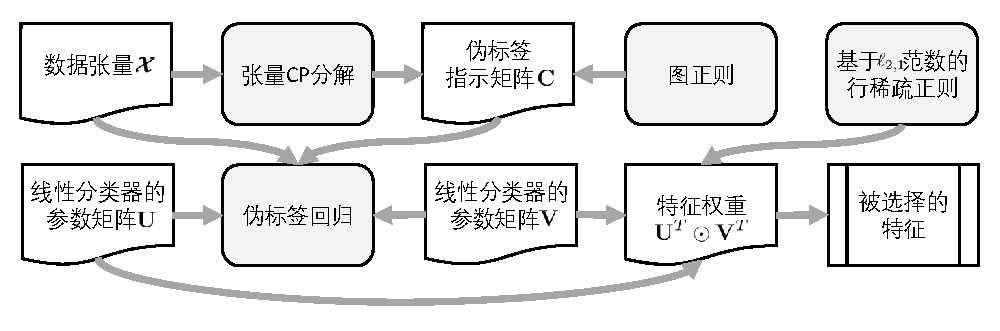
\includegraphics[width=\linewidth]{figures/CPUFS_cn.pdf}
	\caption{CPUFS方法的流程示意图}
	\label{fig:CPUFS-routine}
\end{figure}
\vspace{-0.5em}

\section{CPUFS方法的优化模型}
\esection{The Optimization Model of the CPUFS Method}
本节将给出CPUFS方法的优化模型。本节将首先提出全新的面向张量的线性分类器与特征选择矩阵。

\subsection{面向张量的线性分类器设计}\label{sec:design-classf}
\esubsection{Design of Tensor-Oriented Linear Classifier}
为了保留张量的内在结构信息,本文使用张量mode-$n$积来设计面向张量的线性分类器
% \footnote{值得一提的是,另一种常用的张量的乘积——张量收缩积\ucite{bader2006algorithm}并不能被用来设计面向张量的线性分类器。这是由于张量收缩积会破坏张量的结构信息。}
,从而保留张量的内在结构。具体而言,给定三阶张量$\mathbfcal{X}\in\mathbb{R}^{n_{1}\times n_{2}\times n}$,本文很自然地把线性分类器设计为$(\mydiag(\mathbfcal{X}\times_{1}\boldsymbol{U}\times_{2}\boldsymbol{V}))^{\top}\in\mathbb{R}^{n\times c}$,其中$\boldsymbol{U}\in\mathbb{R}^{c\times n_{1}}$和$\boldsymbol{V}\in\mathbb{R}^{c\times n_{2}}$是该线性分类器的两个协同组成部分,而$c$是数据中的潜在类别数。具体而言,对不同的$j=1,2,\ldots,c$,$\boldsymbol{u}_{j:}$和$\boldsymbol{v}_{j:}$协同地且密不可分地通过
\begin{equation*}
    \left[\boldsymbol{u}_{j:}\boldsymbol{X}^{(1)}\boldsymbol{v}_{j:}^{\top},\boldsymbol{u}_{j:}\boldsymbol{X}^{(2)}\boldsymbol{v}_{j:}^{\top}\ldots,\boldsymbol{u}_{j:}\boldsymbol{X}^{(n)}\boldsymbol{v}_{j:}^{\top}\right]^{\top}\in\mathbb{R}^{n},
\end{equation*}
来生成所有样本关于第$j$个类别的聚类伪标签。可以很直观地看到,在这种方式下,张量的内在结构信息被很好地保留了下来。此外,值得一提的是,本文设计的线性分类器的参数量为$\mathcal{O}((n_1+n_2)c)$,而已有方法(如RUFS\ucite{rufs})基于向量化后数据所设计的线性分类器的参数量为$\mathcal{O}(n_1 n_2 c)$。这表明在高维数据环境下,本文设计的线性分类器的参数量远小于已有方法中的线性分类器的参数量!这个特点不仅使得其可以使用更少的存储空间以及进行更快的数值计算,同时还使得其更不容易过拟合。

\subsection{面向张量的特征选择矩阵设计}\label{sec:design-fsmatrix}
\esubsection{Design of Tensor-Oriented Feature Selection Matrix}
特征选择矩阵的设计应满足以下三个要点:
\begin{enumerate}
    \item 特征选择矩阵应依据参数矩阵$\boldsymbol{U}$和$\boldsymbol{V}$来设计;
    \item 特征选择矩阵应能保留张量数据的内在结构信息;
    \item 特征选择矩阵还应能反应每个特征的重要性。
\end{enumerate}
可以看到,设计该特征选择矩阵并非一件易事。本节接下来详细介绍如何解决这个难题。具体来讲,本文独辟蹊径地将特征选择矩阵设计为$(\boldsymbol{U}^{\top}\odot\boldsymbol{V}^{\top})\in\mathbb{R}^{n_{1}n_{2}\times c}$,原因如下。考虑线性分类器的第$(i,j)$个元素
% 设$(\mydiag(\mathbfcal{X}\times_{1}\boldsymbol{U}\times_{2}\boldsymbol{V}))^{\top}$为$\hat{\boldsymbol{C}}$,然后考虑$\hat{\boldsymbol{C}}$的元素$\hat{c}_{ij}$(它的值指示了我们设计的线性分类器是否将第$i$个样本判为第$j$个类别)。$\hat{c}_{ij}$的计算公式如下
% \begin{equation*}
%     \hat{c}_{ij}=\boldsymbol{u}_{j:}\boldsymbol{X}^{(i)}\boldsymbol{v}_{j:}^{\top}=\sum_{h=1}^{n_{1}}\sum_{g=1}^{n_{2}}u_{jh}v_{jg}x_{hgi}.
% \end{equation*}
\begin{equation*}
    \left((\mydiag(\mathbfcal{X}\times_{1}\boldsymbol{U}\times_{2}\boldsymbol{V}))^{\top}\right)_{ij}=\boldsymbol{u}_{j:}\boldsymbol{X}^{(i)}\boldsymbol{v}_{j:}^{\top}=\sum_{h=1}^{n_{1}}\sum_{g=1}^{n_{2}}u_{jh}v_{jg}x_{hgi},
\end{equation*}
其值表明了线性分类器是否将第$i$个样本判为第$j$个类别。在这个表达式中,$x_{hgi}$代表了$\boldsymbol{X}^{(i)}$的第$(h,g)$个特征的数值大小,而$u_{jh}v_{jg}$由于与样本索引$i$无关可以被解释为第$(h,g)$个特征关于第$j$个类别的特征重要性权重。巧合的是,注意到向量$[u_{1h}v_{1g},u_{2h}v_{2g},\ldots,u_{ch}v_{cg}]$恰巧是$(\boldsymbol{U}^{\top}\odot\boldsymbol{V}^{\top})$的第$((h-1)n_{2}+g)$行。此外,这个巧合的对应关系所蕴含的映射
\begin{equation*}
    (h,g)\mapsto (h-1)n_{2}+g:(\mathbb{Z}\cap [1,n_{1}])\times(\mathbb{Z}\cap [1,n_{2}])\rightarrow(\mathbb{Z}\cap [1,n_{1}n_{2}]),
\end{equation*}
显然是双射,即特征选择矩阵$(\boldsymbol{U}^{\top}\odot\boldsymbol{V}^{\top})$的行向量与数据特征之间存在一一对应关系。因此,将特征选择矩阵定义为$(\boldsymbol{U}^{\top}\odot\boldsymbol{V}^{\top})$。

值得一提的是,由于定义的第$(h,g)$个特征关于第$j$个类别的重要性权重$u_{jh}v_{jg}$由$u_{jh}$和$v_{jg}$两部分组成,并且它们分别关联每个数据样本矩阵的第$h$行和第$g$列。那么,对于位于数据样本矩阵的同一行或者同一列上的所有特征,它们之间的特征重要性权重将会产生相互关联。这是本文的方法能够保留张量的结构信息的理论保证。此外,在实验部分的\refsection{sec:visualization}还会展示,这一机制将赋予被选择特征在位置分布上具有显著的空间结构特征。这是已有的无监督特征选择方法所不具备的特点。


\subsection{CPUFS方法的优化模型}\label{sec:opt-model-CPUFS}
\esubsection{The Optimization Model of the CPUFS Method}
至此,所有用于建立CPUFS方法的优化模型的技术工具都已经在前些章节被介绍或设计。本节接下来直接设计CPUFS方法的优化模型,然后逐项解释所设计的优化模型中的每项及每个约束的目的及意义。具体而言,CPUFS方法的优化模型如下
\begin{gather}\label{eq:tensor-based-ufs}
\begin{aligned}
& \underset{\smash[b]{\substack{\mathclap{\boldsymbol{A},\boldsymbol{B},\boldsymbol{C}}\\\mathclap{\boldsymbol{U},\boldsymbol{V},\boldsymbol{Y}}}}}{\min}
& &  \norm{\mathbfcal{X}-\left\llbracket \boldsymbol{A}, \boldsymbol{B}, \boldsymbol{C} \right\rrbracket}_{F}^{2} + \nu\operatorname{Tr}\left(\boldsymbol{C}^{\top}\boldsymbol{L}\boldsymbol{C}\right) \\ \span&& + \alpha\norm{\left(\mydiag\left(\mathbfcal{X}\times_{1}\boldsymbol{U}\times_{2}\boldsymbol{V}\right)\right)^{\top} - \boldsymbol{C}}_{F}^{2} + \beta \norm{\boldsymbol{U}^{\top}\odot\boldsymbol{V}^{\top}}_{2,1}\\
& \text{s.t.}
& & \boldsymbol{A}\in \mathbb{R}_{+}^{n_1 \times c},~\boldsymbol{B}\in \mathbb{R}_{+}^{n_2 \times c},~\boldsymbol{C}\in \mathbb{R}_{+}^{n \times c},~\boldsymbol{C}=\boldsymbol{Y}\left(\boldsymbol{Y}^{\top} \boldsymbol{Y}\right)^{-\frac{1}{2}},~\boldsymbol{Y}\in\{0,1\}^{n\times c},
\end{aligned}
\raisetag{2.33\normalbaselineskip}
\end{gather}
其中$\nu$、$\alpha$和$\beta$是平衡\refopt{eq:tensor-based-ufs}的目标函数中不同项的重要性大小的权重,$c$是数据样本的潜在类别个数,$n$是数据样本的总数量,$\mathbfcal{X}\in\mathbb{R}_{+}^{n_{1}\times n_{2}\times n}$为输入张量,$\boldsymbol{A} \in \mathbb{R}_{+}^{n_{1}\times c}$、$\boldsymbol{B} \in \mathbb{R}_{+}^{n_{2}\times c}$和$\boldsymbol{C} \in \mathbb{R}_{+}^{n\times c}$为非负张量CP分解的因子矩阵,$\boldsymbol{L} \in \mathbb{R}^{n\times n}$为基于\refsection{sec:graphreg}中方法所构建的带权$k$近邻图所对应的拉普拉斯矩阵,而$\boldsymbol{U}\in\mathbb{R}^{c\times n_{1}}$和$\boldsymbol{V}\in\mathbb{R}^{c\times n_{2}}$为线性分类器$\mydiag(\mathbfcal{X}\times_{1}\boldsymbol{U}\times_{2}\boldsymbol{V})$的两个参数矩阵。本节接下来逐项解释\refopt{eq:tensor-based-ufs}中每项及每个约束的目的及意义:
\begin{enumerate}
    \item $\norm{\mathbfcal{X}-\left\llbracket \boldsymbol{A}, \boldsymbol{B}, \boldsymbol{C} \right\rrbracket}_{F}^{2}$(且$\boldsymbol{A}\in \mathbb{R}_{+}^{n_1 \times c}$,$\boldsymbol{B}\in \mathbb{R}_{+}^{n_2 \times c}$,$\boldsymbol{C}\in \mathbb{R}_{+}^{n \times c}$)是张量$\mathbfcal{X}$的非负张量CP分解的目标函数(请参考\refsection{sec:tensor-decomp})。这一项负责通过挖掘张量的内在特性来生成伪标签$\boldsymbol{C}$($\boldsymbol{C}$将会被用于其它子任务),并保留张量$\mathbfcal{X}$中的结构信息。

    \item $\operatorname{Tr}(\boldsymbol{C}^{\top}\boldsymbol{L}\boldsymbol{C})$是图正则的目标函数(请参考\refsection{sec:graphreg})。这一项负责捕获张量样本之间的内在几何结构信息,并驱使着在数据几何结构上相似的样本点具有尽可能相似的伪标签信息。

    \item $\norm{(\mydiag(\mathbfcal{X}\times_{1}\boldsymbol{U}\times_{2}\boldsymbol{V}))^{\top} - \boldsymbol{C}}_{F}^{2}$是线性分类器$\mydiag(\mathbfcal{X}\times_{1}\boldsymbol{U}\times_{2}\boldsymbol{V})$拟合产生的伪标签$\boldsymbol{C}$的目标函数。简单起见,使用Frobenius范数诱导的度量来量化$\mydiag(\mathbfcal{X}\times_{1}\boldsymbol{U}\times_{2}\boldsymbol{V})$与$\boldsymbol{C}$之间的差距。

    \item $\norm{\boldsymbol{U}^{\top}\odot\boldsymbol{V}^{\top}}_{2,1}$是对特征选择矩阵施加行稀疏正则的目标函数。
    这一项迫使特征选择矩阵的行向量变得稀疏。
    由于特征选择矩阵的每一行编码了不同特征的重要性权重,因此若其某一行的$\ell_{2}$范数越小,则与该行所对应的特征对于拟合伪标签$\boldsymbol{C}$起到的作用也就越小,那么该特征也就越不重要。
    % 因此,可以通过比较特征选择矩阵的行$\ell_{2}$范数大小来选择更高质量的特征。
    % After \refopt{eq:tensor-based-ufs} has been well optimized, we can select features according to the $\ell_{2}$-norms of rows of $(\boldsymbol{U}^{\top}\odot\boldsymbol{V}^{\top})$.
    % Thus, we can select discriminative features according to the $\ell_{2}$-norms of rows of $(\boldsymbol{U}^{\top}\odot\boldsymbol{V}^{\top})$.
    % Therefore, minimizing $\norm{\boldsymbol{U}^{\top}\odot\boldsymbol{V}^{\top}}_{2,1}$ has the functionality to filter out those less important features.

    \item $\boldsymbol{C}=\boldsymbol{Y}(\boldsymbol{Y}^{\top} \boldsymbol{Y})^{-\frac{1}{2}}$(且$\boldsymbol{Y}\in\{0,1\}^{n\times c}$)是迫使产生的伪标签矩阵$\boldsymbol{C}$成为归一化的类指示矩阵的离散约束。
    此处引入二值矩阵$\boldsymbol{Y}\in\{0,1\}^{n\times c}$来描述数据集$\mathcal{D}_{\text{特征选择}}$中的样本-类簇关系,并定义归一化的类指示矩阵为$\Tilde{\boldsymbol{Y}}=\boldsymbol{Y}(\boldsymbol{Y}^{\top} \boldsymbol{Y})^{-1/2}$,而$\Tilde{\boldsymbol{Y}}$与$\boldsymbol{Y}$相比性质更好\ucite{udfs, ndfs, rufs}(例如注意到$\Tilde{\boldsymbol{Y}}^{\top} \Tilde{\boldsymbol{Y}}\allowbreak=(\boldsymbol{Y}^{\top} \boldsymbol{Y})^{-1/2} \boldsymbol{Y}^{\top} \boldsymbol{Y}(\boldsymbol{Y}^{\top} \boldsymbol{Y})^{-1/2}=\boldsymbol{I}_{c}$)。
    % 约束$\boldsymbol{C}$成为归一化的聚类指示矩阵,从而更贴合实际并具有更好性质。
    % 关于归一化的聚类指示矩阵的定义及其意义
\end{enumerate}

总体来看,在\refopt{eq:tensor-based-ufs}中,目标函数的前两项(即上文的1和2)负责在保留张量局部几何结构及其内在结构信息的同时产生高质量的数据伪标签,而目标函数的后两项(即上文的3、4和5)则负责通过线性分类器拟合数据伪标签并基于此实现特征重要性权重的稀疏化。这两个过程将会在训练过程中相互引导对方,以实现更好的效果。然而,由于\refopt{eq:tensor-based-ufs}的约束项存在离散约束,求解的难度实际上是很大的。为了解决这个问题,需要对该优化问题进行一些必要的松弛和等价变换。下一节将讨论这些策略。

% 为了处理张量,几乎所有现有的无监督特征选择方法都牺牲了张量的结构信息以换取数据处理的简单性。但是,这些信息可能是非常重要的。例如,它们可能能为张量分类提供判别信息。然而,我们提出的CPUFS方法利用非负张量CP分解来生成伪分类标签,并使用新设计的面向张量的线性分类器以及特征选择矩阵来进行伪标签回归以及特征权重稀疏化,从而在整个过程中都保留了张量的数据结构信息。


\section{CPUFS方法的优化算法及其理论分析}
\esection{The Optimization Algorithm for Solving the CPUFS Method with Its Theoretical Analysis}
本节将设计一种求解CPUFS方法的高效优化算法,并对该算法进行理论上的收敛性分析以及计算复杂度分析。
\subsection{CPUFS方法的松弛}
\esubsection{Relaxations for the CPUFS Method}
\refopt{eq:tensor-based-ufs}的难点主要在于涉及离散矩阵的约束$\boldsymbol{C}=\boldsymbol{Y}(\boldsymbol{Y}^{\top} \boldsymbol{Y})^{-\frac{1}{2}}$以及$\boldsymbol{Y}\in\{0,1\}^{n\times c}$。为了解决上述难点,需要将矩阵$\boldsymbol{C}$松弛为连续矩阵。尽管如此,直接松弛$\boldsymbol{C}$为连续矩阵可能会带来严重的后果。比方说,如果直接松弛$\boldsymbol{C}$为连续矩阵而不施加任何约束,那么最优的$\boldsymbol{C}$很有可能会是非常稠密的矩阵,但这降低了其作为数据伪标签指示矩阵的效用性,因为希望每个样本具有清晰的聚类隶属度。注意到,在原有约束中,矩阵$\boldsymbol{C}$还有额外的性质,即$\boldsymbol{C}^{\top}\boldsymbol{C}=\boldsymbol{I}_{c}$。该性质可以帮助摆脱绝大多数不理想的解,原因在于:根据文献\ucite{ding2005equivalence},由于正交约束和非负约束的同时存在,矩阵$\boldsymbol{C}$的每行中都只可能存在一个非零元素,且该元素指示了对应于该行的样本的分类情况。
% 该属性摆脱了非负张量CP分解的因子矩阵的稠密本质,从而为其它组成模组提供更具判别性的伪分类标签。
因此,将\refopt{eq:tensor-based-ufs}松弛为如下优化问题
\begin{equation*}
\begin{aligned}
& \underset{\smash[b]{\substack{\mathclap{\boldsymbol{A},\boldsymbol{B},\boldsymbol{C},}\\\mathclap{\boldsymbol{U},\boldsymbol{V}}}}}{\min}
& &  \norm{\mathbfcal{X}-\left\llbracket \boldsymbol{A}, \boldsymbol{B}, \boldsymbol{C} \right\rrbracket}_{F}^{2} + \nu\operatorname{Tr}\left(\boldsymbol{C}^{\top}\boldsymbol{L}\boldsymbol{C}\right) \\ \span&& + \alpha\norm{\left(\mydiag\left(\mathbfcal{X}\times_{1}\boldsymbol{U}\times_{2}\boldsymbol{V}\right)\right)^{\top} - \boldsymbol{C}}_{F}^{2} + \beta \norm{\boldsymbol{U}^{\top}\odot\boldsymbol{V}^{\top}}_{2,1}\\
& \text{s.t.}
& & \boldsymbol{A}\in \mathbb{R}_{+}^{n_1 \times c},~\boldsymbol{B}\in \mathbb{R}_{+}^{n_2 \times c},~\boldsymbol{C}\in \mathbb{R}_{+}^{n \times c},~\boldsymbol{C}^{\top}\boldsymbol{C} = \boldsymbol{I}_{c}.
\end{aligned}
\end{equation*}
然而,尽管已经做了一些松弛,同时施加在矩阵$\boldsymbol{C}$上的非负约束和正交约束仍然使得目标函数难以优化。受到文献\ucite{socfs}的启发,本节提出了另一个等价的优化问题
\begin{equation*}\label{eq:cpufs-equiv}
    \begin{aligned}
    & \underset{\smash[b]{\substack{\mathclap{\boldsymbol{A},\boldsymbol{B},\boldsymbol{C},}\\\mathclap{\boldsymbol{F},\boldsymbol{U},\boldsymbol{V}}}}}{\min}
    & &  \norm{\mathbfcal{X}-\left\llbracket \boldsymbol{A}, \boldsymbol{B}, \boldsymbol{C} \right\rrbracket}_{F}^{2} + \nu\operatorname{Tr}\left(\boldsymbol{C}^{\top}\boldsymbol{L}\boldsymbol{F}\right) \\ \span&& + \alpha\norm{\left(\mydiag\left(\mathbfcal{X}\times_{1}\boldsymbol{U}\times_{2}\boldsymbol{V}\right)\right)^{\top} - \boldsymbol{F}}_{F}^{2} + \beta \norm{\boldsymbol{U}^{\top}\odot\boldsymbol{V}^{\top}}_{2,1}\\
    & \text{s.t.}
    & & \boldsymbol{A}\in \mathbb{R}_{+}^{n_1 \times c},~\boldsymbol{B}\in \mathbb{R}_{+}^{n_2 \times c},~\boldsymbol{F}\in \mathbb{R}_{+}^{n \times c},~\boldsymbol{F}=\boldsymbol{C},~\boldsymbol{C}^{\top}\boldsymbol{C} = \boldsymbol{I}_{c},
    \end{aligned}
\end{equation*}
其中$\boldsymbol{F}$为辅助矩阵。
% 它旨在
% \begin{enumerate*}[label=(\arabic*)]
%     \item 替矩阵$\boldsymbol{C}$分担之前施加在它上面的非负约束$\boldsymbol{C}\geq 0$,以及
%     \item 将目标函数中的$\operatorname{Tr}(\boldsymbol{C}^{\top}\boldsymbol{L}\boldsymbol{C})$以及$\Vert(\mydiag(\mathbfcal{X}\times_{1}\boldsymbol{U}\times_{2}\boldsymbol{V}))^{\top} - \boldsymbol{C}\Vert_{F}^{2}$分别转化为更容易优化的$\operatorname{Tr}(\boldsymbol{C}^{\top}\boldsymbol{L}\boldsymbol{F})$和$\Vert(\mydiag(\mathbfcal{X}\times_{1}\boldsymbol{U}\times_{2}\boldsymbol{V}))^{\top} - \boldsymbol{F}\Vert_{F}^{2}$。
% \end{enumerate*}
通过定义度量违反约束$\boldsymbol{F}=\boldsymbol{C}$的程度的罚函数$\norm{\boldsymbol{C}-\boldsymbol{F}}_{F}^{2}$,并将该罚函数叠加到目标函数上去,可以将上述优化问题转化为以下更易求解的优化问题
\begin{gather}\label{eq:alterobj}
\begin{aligned}
& \underset{\smash[b]{\substack{\mathclap{\boldsymbol{A},\boldsymbol{B},\boldsymbol{C},}\\\mathclap{\boldsymbol{F},\boldsymbol{U},\boldsymbol{V}}}}}{\min}
& &  \norm{\mathbfcal{X}-\left\llbracket \boldsymbol{A}, \boldsymbol{B}, \boldsymbol{C} \right\rrbracket}_{F}^{2} + \nu\operatorname{Tr}\left(\boldsymbol{C}^{\top}\boldsymbol{L}\boldsymbol{F}\right) + \eta\norm{\boldsymbol{C}-\boldsymbol{F}}_{F}^{2} \\ \span&& + \alpha\norm{\left(\mydiag\left(\mathbfcal{X}\times_{1}\boldsymbol{U}\times_{2}\boldsymbol{V}\right)\right)^{\top} - \boldsymbol{F}}_{F}^{2} + \beta \norm{\boldsymbol{U}^{\top}\odot\boldsymbol{V}^{\top}}_{2,1}\\
& \text{s.t.}
& & \boldsymbol{A}\in \mathbb{R}_{+}^{n_1 \times c},~\boldsymbol{B}\in \mathbb{R}_{+}^{n_2 \times c},~\boldsymbol{F}\in \mathbb{R}_{+}^{n \times c},~\boldsymbol{C}^{\top}\boldsymbol{C} = \boldsymbol{I}_{c},
\end{aligned}
\end{gather}
其中$\eta$是足够大的常数,用以保证$\boldsymbol{F}$和$\boldsymbol{C}$在数值上足够接近。
至此,CPUFS方法的优化难度已经被大大降低,即现在每个优化变量只有至多一个约束。
% 然而,尽管CPUFS方法已经得到松弛,
% 尽管如此,由于\refopt{eq:alterobj}仍然为非常复杂的优化问题,因而不可能直接找到它的全局最优解。
尽管如此,仍然不可能直接找到\refopt{eq:alterobj}的全局最优解。
因此,下一节将基于迭代优化的策略设计一种优化算法用以求解\refopt{eq:alterobj}。

\subsection{优化算法设计}
\esubsection{Design of the Optimization Algorithm}
本节设计一种用于求解\refopt{eq:alterobj}的高效迭代优化算法。本节接下来依次推导各个优化变量的更新公式。

\textbf{$\boldsymbol{A}$的更新:}通过简单的代数运算以及应用\refsection{sec:tensor-decomp}中介绍的mode-$k$展开技巧,仅与$\boldsymbol{A}$有关的子问题即为以下非负矩阵分解问题\ucite{lee2001algorithms}
\begin{equation*}
    \begin{aligned}
    &\underset{\mathclap{\boldsymbol{A}}}{\min}\Hquad &&\norm{\boldsymbol{X}_{\left(1\right)}-\boldsymbol{A}\left(\boldsymbol{C}\odot\boldsymbol{B}\right)^{\top}}_{F}^{2}\\
    & \text{s.t.} && \boldsymbol{A}\in \mathbb{R}_{+}^{n_1 \times c},
    \end{aligned}
\end{equation*}
% 而这个问题已经被广泛研究。
则可以应用\refsection{sec:nmf-dec}中介绍的Lee-Seung算法\ucite{lee2001algorithms}来更新之,即
\begin{equation*}
% \label{eq:updateA}
    \boldsymbol{A}\leftarrow\boldsymbol{A}\oast\frac{\boldsymbol{X}_{(1)}\left(\boldsymbol{C}\odot\boldsymbol{B}\right)}{\boldsymbol{A}\left(\boldsymbol{C}\odot\boldsymbol{B}\right)^{\top}\left(\boldsymbol{C}\odot\boldsymbol{B}\right)}.
\end{equation*}

\textbf{$\boldsymbol{B}$的更新:}与$\boldsymbol{A}$子问题类似,仅与$\boldsymbol{B}$有关的子问题也为非负矩阵分解问题,即
\begin{equation*}
    \begin{aligned}
    &\underset{\mathclap{\boldsymbol{B}}}{\min}\Hquad &&\norm{\boldsymbol{X}_{\left(2\right)}-\boldsymbol{B}\left(\boldsymbol{C}\odot\boldsymbol{A}\right)^{\top}}_{F}^{2}\\
    & \text{s.t.} && \boldsymbol{B}\in \mathbb{R}_{+}^{n_2 \times c},
    \end{aligned}
\end{equation*}
则可以再次应用Lee-Seung算法的来更新之,即
\begin{equation*}
% \label{eq:updateB}
    \boldsymbol{B}\leftarrow\boldsymbol{B}\oast\frac{\boldsymbol{X}_{(2)}\left(\boldsymbol{C}\odot\boldsymbol{A}\right)}{\boldsymbol{B}\left(\boldsymbol{C}\odot\boldsymbol{A}\right)^{\top}\left(\boldsymbol{C}\odot\boldsymbol{A}\right)}.
\end{equation*}

\textbf{$\boldsymbol{C}$的更新:}仅与$\boldsymbol{C}$有关的子问题为
\begin{equation*}
    \begin{aligned}
    &\underset{\boldsymbol{C}}{\min} \Hquad &&\norm{\boldsymbol{X}_{\left(3\right)}-\boldsymbol{C}\left(\boldsymbol{B}\odot\boldsymbol{A}\right)^{\top}}_{F}^{2} + \nu\operatorname{Tr}\left(\boldsymbol{C}^{\top}\boldsymbol{L}\boldsymbol{F}\right) + \eta\norm{\boldsymbol{C}-\boldsymbol{F}}_{F}^{2}\\
    & \text{s.t.} && \boldsymbol{C}^{\top}\boldsymbol{C}=\boldsymbol{I}_{c},
    \end{aligned}
\end{equation*}
而这个子问题可以被进一步等价为正交普鲁克问题\ucite{viklands2006algorithms}的特例
\begin{equation*}
    \begin{aligned}
    &\underset{\boldsymbol{C}}{\min} \Hquad &&\norm{\boldsymbol{C} - \left(2\boldsymbol{X}_{(3)}\left(\boldsymbol{B}\odot\boldsymbol{A}\right) - \nu\boldsymbol{L}\boldsymbol{F} + 2\eta\boldsymbol{F}\right)}_{F}^{2}\\
    & \text{s.t.} && \boldsymbol{C}^{\top}\boldsymbol{C}=\boldsymbol{I}_{c}.
    \end{aligned}
\end{equation*}
% 而该问题为正交普鲁克问题\ucite{viklands2006algorithms}的特例。

\begin{lemma}[正交普鲁克问题的解\ucite{viklands2006algorithms}]\kaishu
\label{lemma:quad}
给定矩阵$\boldsymbol{P} \in \mathbb{R}^{n \times m}$和$\boldsymbol{Q} \in \mathbb{R}^{n \times d}$,则优化问题
\begin{equation*}
    \begin{aligned}
&\underset{\mathclap{\Tilde{\boldsymbol{T}}}}{\min} \Hquad&&\left\|\boldsymbol{P}\boldsymbol{\Tilde{T}}-\boldsymbol{Q}\right\|_{F}^{2}\\
&\text{s.t.} && \Tilde{\boldsymbol{T}}\Tilde{\boldsymbol{T}}^{\top} = \boldsymbol{I}_{m},
\end{aligned}
\end{equation*}
有如下解析解
\begin{equation*}
    \Tilde{\boldsymbol{T}}=\boldsymbol{U}\boldsymbol{I}_{m,d}\boldsymbol{V}^{\top},
\end{equation*}
其中$\boldsymbol{U} \in \mathbb{R}^{m \times m}$和$\boldsymbol{V} \in \mathbb{R}^{d \times d}$分别为$\boldsymbol{P}^{\top}\boldsymbol{Q}$的奇异值分解的左右奇异矩阵。
\end{lemma}
\noindent 如果令$\boldsymbol{P}=\boldsymbol{I}_{c}$、$\Tilde{\boldsymbol{T}}=\boldsymbol{C}^{\top}$以及$\boldsymbol{Q}=2(\boldsymbol{B}\odot\boldsymbol{A})^{\top}\boldsymbol{X}_{(3)}^{\top}-\nu\boldsymbol{F}^{\top}\boldsymbol{L}^{\top} + 2\eta\boldsymbol{F}^{\top}$,
% \begin{equation*}
%     \boldsymbol{P}=\boldsymbol{I}_{c},~
%     \Tilde{\boldsymbol{T}}=\boldsymbol{C}^{\top},~\text{以及}~
%     \boldsymbol{Q}=2(\boldsymbol{B}\odot\boldsymbol{A})^{\top}\boldsymbol{X}_{(3)}^{\top}-\nu\boldsymbol{F}^{\top}\boldsymbol{L}^{\top} + 2\eta\boldsymbol{F}^{\top},
% \end{equation*}
那么\reflemma{lemma:quad}中的优化问题将与$\boldsymbol{C}$子问题一致。由此,利用\reflemma{lemma:quad}可以得到$\boldsymbol{C}$子问题的最优更新方式,即
\begin{equation*}
% \label{eq:updateC}
    \boldsymbol{C} \leftarrow \boldsymbol{V}_{\boldsymbol{C}}\boldsymbol{I}_{n,c}\boldsymbol{U}_{\boldsymbol{C}}^{\top},
\end{equation*}
其中$\boldsymbol{U}_{\boldsymbol{C}}$和$\boldsymbol{V}_{\boldsymbol{C}}$分别为$2(\boldsymbol{B}\odot\boldsymbol{A})^{\top}\boldsymbol{X}_{(3)}^{\top}-\nu\boldsymbol{F}^{\top}\boldsymbol{L}^{\top} + 2\eta\boldsymbol{F}^{\top}$的奇异值分解的左右奇异矩阵。

\textbf{$\boldsymbol{F}$的更新:}仅与$\boldsymbol{F}$有关的子问题为
\begin{equation*}
\begin{aligned}
    &\underset{\mathclap{\boldsymbol{F}}}{\min} \Hquad &&\alpha\norm{\left(\mydiag\left(\mathbfcal{X}\times_{1}\boldsymbol{U}\times_{2}\boldsymbol{V}\right)\right)^{\top} - \boldsymbol{F}}_{F}^{2} + \nu\operatorname{Tr}\left(\boldsymbol{C}^{\top}\boldsymbol{L}\boldsymbol{F}\right) + \eta\norm{\boldsymbol{C}-\boldsymbol{F}}_{F}^{2}\\
    & \text{s.t.} && \boldsymbol{F}\in \mathbb{R}_{+}^{n \times c},
\end{aligned}
\end{equation*}
而这个子问题可以被进一步等价为
\begin{equation*}
    \begin{aligned}
    &\underset{\mathclap{\boldsymbol{F}}}{\min} \Hquad &&\norm{\boldsymbol{F}-\frac{\alpha\left(\mydiag\left(\mathbfcal{X}\times_{1}\boldsymbol{U}\times_{2}\boldsymbol{V}\right)\right)^{\top}+\eta\boldsymbol{C} -\frac{\nu}{2}\boldsymbol{L}^{\top}\boldsymbol{C}}{\alpha+\eta} }_{F}^{2}\\
    & \text{s.t.} && \boldsymbol{F}\in \mathbb{R}_{+}^{n \times c},
    \end{aligned}
\end{equation*}
很明显,$\boldsymbol{F}$子问题的最优更新方式为
\begin{equation}
\label{eq:updateF}
    \boldsymbol{F}\leftarrow\frac{1}{\alpha+\eta}\left(\alpha\left(\mydiag\left(\mathbfcal{X}\times_{1}\boldsymbol{U}\times_{2}\boldsymbol{V}\right)\right)^{\top} +\eta\boldsymbol{C}-\frac{\nu}{2}\boldsymbol{L}^{\top}\boldsymbol{C}\right)_{+}.
\end{equation}

\textbf{$\boldsymbol{U}$和$\boldsymbol{V}$的更新:}仅与$\boldsymbol{U}$和$\boldsymbol{V}$有关的子问题为
\begin{equation*}
% \hspace{-1em}
    \underset{\mathclap{\boldsymbol{U},\boldsymbol{V}}}{\min} \quad \alpha\norm{\left(\mydiag\left(\mathbfcal{X}\times_{1}\boldsymbol{U}\times_{2}\boldsymbol{V}\right)\right)^{\top} - \boldsymbol{F}}_{F}^{2} + \beta \norm{\boldsymbol{U}^{\top}\odot\boldsymbol{V}^{\top}}_{2,1}.
\end{equation*}
可以发现,这是无约束的优化问题。该优化问题的目标函数具有一些良好的性质,见下面的定理。
\begin{theorem}\label{thm:UVcvx}\kaishu
    函数
    \begin{equation*}
        \alpha\norm{\left(\mydiag\left(\mathbfcal{X}\times_{1}\boldsymbol{U}\times_{2}\boldsymbol{V}\right)\right)^{\top} - \boldsymbol{F}}_{F}^{2} + \beta \norm{\boldsymbol{U}^{\top}\odot\boldsymbol{V}^{\top}}_{2,1},
    \end{equation*}
    关于矩阵$\boldsymbol{U}$(或$\boldsymbol{V}$)是凸的。
\end{theorem}
\noindent 为了证明这个定理,首先证明以下若干引理。
\begin{lemma}\label{lemma:UVcvx1}\kaishu
    $\norm{(\mydiag(\mathbfcal{X}\times_{1}\boldsymbol{U}\times_{2}\boldsymbol{V}))^{\top} - \boldsymbol{F}}_{F}^{2}$关于矩阵$\boldsymbol{U}$(或$\boldsymbol{V}$)是凸的。
\end{lemma}

\begin{proof}
    显然,$\boldsymbol{U}\mapsto(\mydiag(\mathbfcal{X}\times_{1}\boldsymbol{U}\times_{2}\boldsymbol{V}))^{\top} - \boldsymbol{F}$是矩阵$\boldsymbol{U}$的仿射函数。此外,由于Frobenius范数是一种范数,所以$\norm{\cdot}_{F}^{2}$是凸函数
    % \footnote{这并不是显然的结果。这是由于$\boldsymbol{X}\mapsto\norm{\boldsymbol{X}}_{F}^{2}:\mathbb{R}^{m\times n}\rightarrow\mathbb{R}_{+}$可以看作是凸函数$g(\boldsymbol{X})=\norm{\boldsymbol{X}}_{F}:\mathbb{R}^{m\times n}\rightarrow:\mathbb{R}_{+}$和凸函数$f(x)=x^{2}:\mathbb{R}_{+}\rightarrow\mathbb{R}_{+}$的复合函数$f\circ g$,并且$f(x)$在其定义域上是非递减的,因而由文献\ucite{boyd2004convex}即可得上述断言。}
    。由于凸函数与仿射函数的复合函数仍然是凸函数\ucite{boyd2004convex},那么可以推出$\lVert(\mydiag(\mathbfcal{X}\times_{1}\boldsymbol{U}\times_{2}\boldsymbol{V}))^{\top} \allowbreak - \boldsymbol{F}\rVert_{F}^{2}$关于矩阵$\boldsymbol{U}$是凸的。同样地,也可以推出,$\norm{(\mydiag(\mathbfcal{X}\times_{1}\boldsymbol{U}\times_{2}\boldsymbol{V}))^{\top} - \boldsymbol{F}}_{F}^{2}$关于矩阵$\boldsymbol{V}$也是凸的。
\end{proof}\vspace{0.5em}

% \begin{proof}
%     我们首先证明$\norm{(\mydiag(\mathbfcal{X}\times_{1}\boldsymbol{U}\times_{2}\boldsymbol{V}))^{\top} - \boldsymbol{F}}_{F}^{2}$对矩阵$\boldsymbol{U}$的每一行$\boldsymbol{u}_{i:}$都是凸的。简单的计算表明
%     \begin{equation*}
%         \nabla_{\boldsymbol{u}_{i:}}^{2}\left(\norm{\left(\mydiag\left(\mathbfcal{X}\times_{1}\boldsymbol{U}\times_{2}\boldsymbol{V}\right)\right)^{\top} - \boldsymbol{F}}_{F}^{2}\right) = 2\sum_{k=1}^{n}\boldsymbol{X}^{(k)}\boldsymbol{v}_{i:}^{\top}\boldsymbol{v}_{i:}{\boldsymbol{X}^{(k)}}^{\top}\succeq 0.
%     \end{equation*}
%     因此,我们可以得出以下结论:$\norm{(\mydiag(\mathbfcal{X}\times_{1}\boldsymbol{U}\times_{2}\boldsymbol{V}))^{\top} - \boldsymbol{F}}_{F}^{2}$对矩阵$\boldsymbol{U}$的每一行$\boldsymbol{u}_{i:}$都是凸的。同样地,我们也可以证明$\norm{(\mydiag(\mathbfcal{X}\times_{1}\boldsymbol{U}\times_{2}\boldsymbol{V}))^{\top} - \boldsymbol{F}}_{F}^{2}$对矩阵$\boldsymbol{V}$的每一行$\boldsymbol{v}_{i:}$也都是凸的。我们在此处省略证明,以防赘述。
% \end{proof}\vspace{0.5em}

% \begin{lemma}\kaishu
%     $\norm{(\mydiag(\mathbfcal{X}\times_{1}\boldsymbol{U}\times_{2}\boldsymbol{V}))^{\top} - \boldsymbol{F}}_{F}^{2}$分别关于矩阵$\boldsymbol{U}$或$\boldsymbol{V}$都是凸的。
% \end{lemma}

% \begin{proof}
%     这是由于我们有
%     \begin{equation*}
%     \begin{aligned}
%         &\norm{\left(\mydiag\left(\mathbfcal{X}\times_{1}\left(\lambda\boldsymbol{Z}_{1}+\left(1-\lambda\right)\boldsymbol{Z}_{2}\right)\times_{2}\boldsymbol{V}\right)\right)^{\top} - \boldsymbol{F}}_{F}^{2} \\=& \sum_{i=1}^{c}\norm{\left(\mydiag\left(\mathbfcal{X}\times_{1}\left(\lambda(\boldsymbol{z}_{1})_{i:}+\left(1-\lambda\right)(\boldsymbol{z}_{2})_{i:}\right)\times_{2}\boldsymbol{v}_{i:}\right)\right)^{\top} - \boldsymbol{f}_{i}}_{F}^{2} \\\leq& \sum_{i=1}^{c}\left(\lambda\norm{\left(\mydiag\left(\mathbfcal{X}\times_{1}(\boldsymbol{z}_{1})_{i:}\times_{2}\boldsymbol{v}_{i:}\right)\right)^{\top} - \boldsymbol{f}_{i}}_{F}^{2} + \left(1-\lambda\right)\norm{\left(\mydiag\left(\mathbfcal{X}\times_{1}(\boldsymbol{z}_{2})_{i:}\times_{2}\boldsymbol{v}_{i:}\right)\right)^{\top} - \boldsymbol{f}_{i}}_{F}^{2}\right)\\=& \lambda\norm{\left(\mydiag\left(\mathbfcal{X}\times_{1}\boldsymbol{Z}_{1}\times_{2}\boldsymbol{V}\right)\right)^{\top} - \boldsymbol{F}}_{F}^{2} + \left(1-\lambda\right)\norm{\left(\mydiag\left(\mathbfcal{X}\times_{1}\boldsymbol{Z}_{2}\times_{2}\boldsymbol{V}\right)\right)^{\top} - \boldsymbol{F}}_{F}^{2},
%     \end{aligned}
%     \end{equation*}
%     其中不等号部分使用了\reflemma{lemma:thm0}。依据凸函数的定义\ucite{boyd2004convex},$\boldsymbol{U}$部分的证明就完成了。同样的证明方法也可应用在$\boldsymbol{V}$上。为了避免冗余,我们不再赘述。
% \end{proof}\vspace{0.5em}

\begin{lemma}\kaishu
    $\boldsymbol{X}\mapsto\norm{\boldsymbol{X}}_{2,1}:\mathbb{R}^{m\times n}\rightarrow\mathbb{R}_{+}$是关于$\boldsymbol{X}$的凸函数。
\end{lemma}

\begin{proof}
    由于所有的范数都是凸的\ucite{boyd2004convex},因此只需要证明$\ell_{2,1}$范数的确是一种范数即可
%     \footnote{尽管从名字上来看,$\ell_{2,1}$范数似乎就是一种范数,但其实这是需要证明的。例如,$\forall~0\leq p < 1$,虽然都称$\ell_{p}$范数为“范数”,但其实它们并不满足范数的条件。简单的反证法表明,如果它们满足范数的条件,那么它们的下水平集都是凸集。考虑赋范空间$(\mathbb{R}^{d},\norm{\cdot}_{p})$中的单位圆盘$\mathbb{B}_{p}(0,1):=\{\boldsymbol{x}\in\mathbb{R}^{d}\mid\norm{x}_{p}\leq 1\}$,则$\mathbb{B}_{p}(0,1)$为$\ell_{p}$范数的一个下水平集。但由下图所展示的$\{(\mathbb{R}^{2},\norm{\cdot}_{p})\}_{p=1,2,\infty,1/2}$中的单位圆盘(或凭经验)即可得知当$d=2$时,$\forall~0\leq p < 1$,$\mathbb{B}_{p}(0,1)$显然均非凸集。因此$\forall~0\leq p < 1$,$\ell_{p}$范数均不是范数。
%     \begin{center}
%     \resizebox{.8\linewidth}{!}{\begin{tikzpicture}[>=Stealth]
%   \foreach \i in {0,...,3}{
%      \begin{scope}[xshift=\i*3.5cm]
%       \draw [->] (-1.5,0)--(1.5,0);
%       \draw [->] (0,-1.5)--(0,1.5);
%     \end{scope}
%   }
%   \begin{scope}[draw=black]
%      \draw [pattern={Lines[angle=-45,distance=4pt]}] (-1,0)--(0,1)--(1,0)--(0,-1)--cycle;
%      \draw [pattern={Lines[angle=-45,distance=4pt]}](3.5,0) circle (0.88cm);
%      \draw [pattern={Lines[angle=-45,distance=4pt]},xshift=7cm] (-.66,-.66) rectangle (.66,.66);
%      \begin{scope}[xshift=10.5cm]
%       \draw [domain=0:90,samples=100,smooth,variable=\t] plot({-1*cos(\t)^(3)},{1*sin(\t)^(3)});
%       \draw [domain=0:90,samples=100,smooth,variable=\t] plot({-1*cos(\t)^(3)},{-1*sin(\t)^(3)});
%       \draw [domain=0:90,samples=100,smooth,variable=\t] plot({1*cos(\t)^(3)},{-1*sin(\t)^(3)});
%       \draw [domain=0:90,samples=100,smooth,variable=\t] plot({1*cos(\t)^(3)},{1*sin(\t)^(3)});
%      \end{scope}
%      \draw[pattern={Lines[angle=-45,distance=4pt]},xshift=10.5cm] plot[smooth, samples=100, domain=0:90,variable=\t] ({-1*cos(\t)^(3)},{1*sin(\t)^(3)}) -| (0,0) -- cycle;
%      \draw[pattern={Lines[angle=-45,distance=4pt]},xshift=10.5cm] plot[smooth, samples=100, domain=0:90,variable=\t] ({-1*cos(\t)^(3)},{-1*sin(\t)^(3)}) -| (0,0) -- cycle;
%      \draw[pattern={Lines[angle=-45,distance=4pt]},xshift=10.5cm] plot[smooth, samples=100, domain=0:90,variable=\t] ({1*cos(\t)^(3)},{-1*sin(\t)^(3)}) -| (0,0) -- cycle;
%      \draw[pattern={Lines[angle=-45,distance=4pt]},xshift=10.5cm] plot[smooth, samples=100, domain=0:90,variable=\t] ({1*cos(\t)^(3)},{1*sin(\t)^(3)}) -| (0,0) -- cycle;
%   \end{scope}
%   \foreach \i [count=\j from 0] in {1,2,\infty,\frac{1}{2}} \scoped [xshift=\j*3.5cm] { \node [draw=none,anchor=mid west] at (0.25,-1) {$p=\i$}; };
% \end{tikzpicture}}\end{center}}
。简单的计算表明:
    \begin{itemize}
        \item $\norm{\boldsymbol{0}_{m,n}}_{2,1}=0$,
        \item 若$\boldsymbol{X}\in\mathbb{R}^{m\times n}$,则$\norm{\alpha\boldsymbol{X}}_{2,1}=\sum_{j=1}^{m}\norm{\alpha\boldsymbol{x}_{j:}}_{2}=\alpha\sum_{j=1}^{m}\norm{\boldsymbol{x}_{j:}}_{2}=\alpha\norm{\boldsymbol{X}}_{2,1}$,
        \item 若$\boldsymbol{X},\boldsymbol{Y}\in\mathbb{R}^{m\times n}$,则$\norm{\boldsymbol{X}+\boldsymbol{Y}}_{2,1}=\sum_{j=1}^{m}\norm{\boldsymbol{x}_{j:}+\boldsymbol{y}_{j:}}_{2}\leq\sum_{j=1}^{m}\norm{\boldsymbol{x}_{j:}}_{2}+\sum_{j=1}^{m}\norm{\boldsymbol{y}_{j:}}_{2}=\norm{\boldsymbol{X}}_{2,1}+\norm{\boldsymbol{Y}}_{2,1}$,其中不等式的推导使用了$\ell_{2}$范数的三角不等式。
    \end{itemize}
    因此,$\ell_{2,1}$范数的确是一种范数,故$\norm{\boldsymbol{X}}_{2,1}$是关于$\boldsymbol{X}$的凸函数。
\end{proof}\vspace{0.5em}

\begin{lemma}\label{lemma:UVcvx2}\kaishu
    $\norm{\boldsymbol{U}^{\top}\odot\boldsymbol{V}^{\top}}_{2,1}$关于矩阵$\boldsymbol{U}$(或$\boldsymbol{V}$)是凸的。
\end{lemma}

\begin{proof}
    由于
    \begin{equation*}
        \operatorname{vec}\left(\boldsymbol{U}^{\top} \odot \boldsymbol{V}^{\top}\right)=\left(\boldsymbol{I}_{n_{1}c} \odot\left(\boldsymbol{V}^{\top}\left(\boldsymbol{I}_{c} \otimes \boldsymbol{1}^{\top}_{n_{1}}\right)\right)\right)\operatorname{vec}\left(\boldsymbol{U}^{\top}\right),
    \end{equation*}
    因此,$\boldsymbol{U}\mapsto\boldsymbol{U}^{\top}\odot\boldsymbol{V}^{\top}$是矩阵$\boldsymbol{U}$的线性函数。由于凸函数与线性函数的复合函数仍然是凸函数\ucite{boyd2004convex},那么可以推出$\norm{\boldsymbol{U}^{\top}\odot\boldsymbol{V}^{\top}}_{2,1}$关于矩阵$\boldsymbol{U}$是凸的。同样地,也可以推出,$\norm{\boldsymbol{U}^{\top}\odot\boldsymbol{V}^{\top}}_{2,1}$关于矩阵$\boldsymbol{V}$也是凸的。
\end{proof}\vspace{0.5em}

% \begin{corollary}
%     $\alpha\norm{(\mydiag(\mathbfcal{X}\times_{1}\boldsymbol{U}\times_{2}\boldsymbol{V}))^{\top} - \boldsymbol{F}}_{F}^{2} + \beta \norm{\boldsymbol{U}^{\top}\odot\boldsymbol{V}^{\top}}_{2,1}$关于矩阵$\boldsymbol{U}$或$\boldsymbol{V}$分别是凸的。
% \end{corollary}

% \begin{proof}[\reftheorem{thm:UVcvx}的证明]
\vspace{0.5em}\noindent\textbf{\reftheorem{thm:UVcvx}的证明.}
显然,\reftheorem{thm:UVcvx}中的函数为\reflemma{lemma:UVcvx1}与\reflemma{lemma:UVcvx2}中的函数的非负线性组合。由文献\ucite{boyd2004convex},凸函数的非负线性组合仍然还是凸函数,故\reftheorem{thm:UVcvx}得证。 \hfill\qedsymbol
\vspace{0.5em}
% \end{proof}

然而,尽管$\boldsymbol{U}$和$\boldsymbol{V}$的子问题分别都是无约束的凸优化问题,它们的解析解仍然不可能通过一阶最优性条件\ucite{boyd2004convex}来得到。因此,本文采用简单的梯度下降方法来优化$\boldsymbol{U}$和$\boldsymbol{V}$。具体来说,如果用$\mathcal{J}_{\boldsymbol{U},\boldsymbol{V}}$来代表$\boldsymbol{U}$和$\boldsymbol{V}$子问题的目标函数,那么$\mathcal{J}_{\boldsymbol{U},\boldsymbol{V}}$关于$\boldsymbol{U}$和$\boldsymbol{V}$的梯度分别为
\begin{gather}
    \frac{\partial\mathcal{J}_{\boldsymbol{U},\boldsymbol{V}}}{\partial\boldsymbol{U}} =  2\alpha\sum_{k=1}^{n}\operatorname{diag}\left(\boldsymbol{e}_{:k}\right)\boldsymbol{V}{\boldsymbol{X}^{(k)}}^{\top} + \beta\left(\boldsymbol{V}^{\oast 2}\boldsymbol{Q}\right)\oast\boldsymbol{U},\label{eq:grad-U}\\
    \frac{\partial\mathcal{J}_{\boldsymbol{U},\boldsymbol{V}}}{\partial\boldsymbol{V}} =  2\alpha\sum_{k=1}^{n}\operatorname{diag}\left(\boldsymbol{e}_{:k}\right)\boldsymbol{U}\boldsymbol{X}^{(k)} + \beta\left(\boldsymbol{U}^{\oast 2}\boldsymbol{Q}^{\top}\right)\oast\boldsymbol{V}\label{eq:grad-V},
\end{gather}
% \begin{gather}\label{eq:uv-gradient}
% % \hspace{-1.5em}
%     \left\{\begin{array}{l}{\displaystyle},\\ {\displaystyle,}\end{array}\right.
% % \raisetag{.777\normalbaselineskip}
% \end{gather}
% \begin{equation}
%     % \hspace{-2.5em}
%     \frac{\partial\mathcal{J}_{\boldsymbol{U},\boldsymbol{V}}}{\partial\boldsymbol{U}} =  2\alpha\sum_{k=1}^{n}\operatorname{diag}\left(\boldsymbol{e}_{k}\right)\boldsymbol{V}{\boldsymbol{X}^{(k)}}^{\top} + \beta\left(\left(\left(\boldsymbol{V}\oast\boldsymbol{V}\right)\boldsymbol{Q}\right)\oast\boldsymbol{U}\right), \label{eq:derivU}
% \end{equation}
% and
% \begin{equation}
%     % \hspace{-2em}
%     \frac{\partial\mathcal{J}_{\boldsymbol{U},\boldsymbol{V}}}{\partial\boldsymbol{V}} =  2\alpha\sum_{k=1}^{n}\operatorname{diag}\left(\boldsymbol{e}_{k}\right)\boldsymbol{U}\boldsymbol{X}^{(k)} + \beta((\left(\boldsymbol{U}\oast\boldsymbol{U}\right)\boldsymbol{Q}^{\top})\oast\boldsymbol{V}), \label{eq:derivV}
% \end{equation}
% \begin{align}
% % \hspace{-2.5em}
%     \frac{\partial\mathcal{J}_{\boldsymbol{U},\boldsymbol{V}}}{\partial\boldsymbol{U}} = & \alpha\left(2\sum_{k=1}^{n}\operatorname{diag}\left(\boldsymbol{e}_{k}\right)\boldsymbol{V}\left(\boldsymbol{X}^{(k)}\right)^{\top}\right) \nonumber\\ & + \beta\left(\left(\left(\boldsymbol{V}\oast\boldsymbol{V}\right)\boldsymbol{Q}\right)\oast\boldsymbol{U}\right), \label{eq:derivU}
% \end{align}
% and
% \begin{align}
% % \hspace{-2.5em}
%     \frac{\partial\mathcal{J}_{\boldsymbol{U},\boldsymbol{V}}}{\partial\boldsymbol{V}} =  &\alpha\left(2\sum_{k=1}^{n}\operatorname{diag}\left(\boldsymbol{e}_{k}\right)\boldsymbol{U}\boldsymbol{X}^{(k)}\right) \nonumber\\ & + \beta\left(\left(\left(\boldsymbol{U}\oast\boldsymbol{U}\right)\boldsymbol{Q}^{\top}\right)\oast\boldsymbol{V}\right), \label{eq:derivV}
% \end{align}
其中
\begin{equation*}
\boldsymbol{V}^{\oast 2}=\boldsymbol{V}\oast\boldsymbol{V},
~\boldsymbol{E} = \mydiag(\mathbfcal{X}\times_{1}\boldsymbol{U}\times_{2}\boldsymbol{V}) - \boldsymbol{F}^{\top},
\end{equation*}
% \begin{equation*}
%     \boldsymbol{E} = \mydiag(\mathbfcal{X}\times_{1}\boldsymbol{U}\times_{2}\boldsymbol{V}) - \boldsymbol{F}^{\top},
% \end{equation*}
以及
\begin{equation*}
    \boldsymbol{Q}=\bm{1}_{n_{2}}\bm{1}_{n_{1}}^{\top}\oslash\operatorname{vec}_{n_{2},n_{1}}^{-1}(\sqrt{((\boldsymbol{U}^{\top}\odot\boldsymbol{V}^{\top})\oast(\boldsymbol{U}^{\top}\odot\boldsymbol{V}^{\top}))\boldsymbol{1}_{c}}).
\end{equation*}
有了$\frac{\partial\mathcal{J}_{\boldsymbol{U},\boldsymbol{V}}}{\partial\boldsymbol{U}}$与$\frac{\partial\mathcal{J}_{\boldsymbol{U},\boldsymbol{V}}}{\partial\boldsymbol{V}}$的显式表达式,就可以通过梯度下降法优化$\boldsymbol{U}$和$\boldsymbol{V}$。

\begin{algorithm}[t]\setstretch{1.35}
    \begin{algorithmic}[1]
    \REQUIRE 张量$\mathbfcal{X}\in \mathbb{R}^{n_{1}\times n_{2}\times n}$、参数$\eta$、$\nu$、$\alpha$、$\beta$、学习率$\theta$、最大迭代步数$\Phi_1$与$\Phi_2$以及被选择的特征数$p$
    \ENSURE 被选择的$p$个特征
    \STATE 基于输入张量$\mathbfcal{X}$构建带权$k$近邻图(构建方法参照\refsection{sec:graphreg}所述),之后计算该$k$近邻图所对应的拉普拉斯矩阵$\boldsymbol{L}$;
    \STATE 赋$t\leftarrow0$,并随机初始化$\boldsymbol{A}_{t}$, $\boldsymbol{B}_{t}$, $\boldsymbol{C}_{t}$, $\boldsymbol{F}_{t}$, $\boldsymbol{U}_{t}$, $\boldsymbol{V}_{t}$;
    \WHILE{$t<\Phi_{1}$并且外循环未收敛}
    \STATE 更新$\boldsymbol{A}_{t+1}\leftarrow\boldsymbol{A}_{t}\oast((\boldsymbol{X}_{(1)}(\boldsymbol{C}_{t}\odot\boldsymbol{B}_{t}))\oslash(\boldsymbol{A}_{t}(\boldsymbol{C}_{t}\odot\boldsymbol{B}_{t})^{\top}(\boldsymbol{C}_{t}\odot\boldsymbol{B}_{t})))$;
    \STATE 更新$\boldsymbol{B}_{t+1}\leftarrow\boldsymbol{B}_{t}\oast((\boldsymbol{X}_{(2)}(\boldsymbol{C}_{t}\odot\boldsymbol{A}_{t+1}))\oslash(\boldsymbol{B}_{t}(\boldsymbol{C}_{t}\odot\boldsymbol{A}_{t+1})^{\top}(\boldsymbol{C}_{t}\odot\boldsymbol{A}_{t+1})))$;
    \STATE 更新$\boldsymbol{C}_{t+1} \leftarrow \boldsymbol{V}_{\boldsymbol{C}}\boldsymbol{I}_{n,c}\boldsymbol{U}_{\boldsymbol{C}}^{\top}$,其中$\boldsymbol{U}_{\boldsymbol{C}}$和$\boldsymbol{V}_{\boldsymbol{C}}$分别为矩阵$2(\boldsymbol{B}_{t+1}\odot\boldsymbol{A}_{t+1})^{\top}\allowbreak\boldsymbol{X}_{(3)}^{\top}-\nu\boldsymbol{F}_{t}^{\top}\boldsymbol{L}^{\top} + 2\eta\boldsymbol{F}_{t}^{\top}$的奇异值分解的左右奇异矩阵;
    \STATE 更新$\boldsymbol{F}_{t+1}\leftarrow(\alpha(\mydiag(\mathbfcal{X}\times_{1}\boldsymbol{U}_{t}\times_{2}\boldsymbol{V}_{t}))^{\top}+\eta\boldsymbol{C}_{t+1}-(\nu/2)\boldsymbol{L}^{\top}\boldsymbol{C}_{t+1})_{+}/(\alpha+\eta)$;\hspace{-1em}
    \STATE 赋$\tau\leftarrow 0$并赋$\boldsymbol{U}_{\tau}\leftarrow\boldsymbol{U}_{t}$和$\boldsymbol{V}_{\tau}\leftarrow\boldsymbol{V}_{t}$;
    \WHILE{$\tau<\Phi_{2}$并且内循环未收敛}
    \STATE 更新$\boldsymbol{U}_{\tau+1}\leftarrow\boldsymbol{U}_{\tau}-\theta\inlineEval{\frac{\partial\mathcal{J}_{\boldsymbol{U},\boldsymbol{V}}}{\partial\boldsymbol{U}}}{\boldsymbol{U}=\boldsymbol{U}_{\tau},\boldsymbol{V}=\boldsymbol{V}_{\tau},\boldsymbol{F}=\boldsymbol{F}_{t+1}}{}$以及$\boldsymbol{V}_{\tau+1}\leftarrow\boldsymbol{V}_{\tau}-\theta\inlineEval{\frac{\partial\mathcal{J}_{\boldsymbol{U},\boldsymbol{V}}}{\partial\boldsymbol{V}}}{\boldsymbol{U}=\boldsymbol{U}_{\tau+1},\boldsymbol{V}=\boldsymbol{V}_{\tau},\boldsymbol{F}=\boldsymbol{F}_{t+1}}{}$,其中$\frac{\partial\mathcal{J}_{\boldsymbol{U},\boldsymbol{V}}}{\partial\boldsymbol{U}}$, $\frac{\partial\mathcal{J}_{\boldsymbol{U},\boldsymbol{V}}}{\partial\boldsymbol{V}}$分别由\refequation{eq:grad-U}和\refequation{eq:grad-V}计算得到;
    \STATE 赋$\tau\leftarrow\tau+1$;
    \ENDWHILE
    \STATE 更新$\boldsymbol{U}_{t+1}\leftarrow\boldsymbol{U}_{\tau}$以及$\boldsymbol{V}_{t+1}\leftarrow\boldsymbol{V}_{\tau}$;
    \STATE 赋$t\leftarrow t+1$;
    \ENDWHILE
    \RETURN 对应于矩阵$(\boldsymbol{U}_{t}^{\top}\odot\boldsymbol{V}_{t}^{\top})$就$\ell_{2}$范数而言最大$p$行的那$p$个特征;
    \end{algorithmic}
    \captionsetup{labelsep=period,font=bf}
    \caption{CPUFS方法的优化算法}
    \label{alg:cpufs}
\end{algorithm}
    
基于上面的推导,用于求解CPUFS方法的交替迭代优化算法如\refalg{alg:cpufs}所示。总体来讲,\refalg{alg:cpufs}以交替迭代的方式优化CPUFS,直到满足某些收敛条件而停止。具体来讲,\refalg{alg:cpufs}首先构建输入张量的带权$k$近邻图并计算其对应的拉普拉斯矩阵,然后随机初始化所有因子矩阵(第1-2行)。之后,\refalg{alg:cpufs}使用Lee-Seung算法更新矩阵$\boldsymbol{A}$和$\boldsymbol{B}$(第4-5行),以最优的方式更新矩阵$\boldsymbol{C}$和$\boldsymbol{F}$(第6-7行),并使用梯度下降法更新矩阵$\boldsymbol{U}$和$\boldsymbol{V}$(第8-13行)。一旦达到某些收敛条件,\refalg{alg:cpufs}便停止迭代优化过程。最终,\refalg{alg:cpufs}根据矩阵$(\boldsymbol{U}^{\top}\odot\boldsymbol{V}^{\top})$的行$\ell_{2}$范数来选择高质量特征(第16行)。

\subsection{优化算法的收敛性分析}
\esubsection{Convergence Analysis of the Optimization Algorithm}

本节从理论上证明\refalg{alg:cpufs}的收敛性。为方便起见,$\mathcal{J}(\boldsymbol{A},\boldsymbol{B},\allowbreak\boldsymbol{C},\boldsymbol{F},\boldsymbol{U},\boldsymbol{V})$表示\refopt{eq:alterobj}的目标函数。

\begin{theorem}\label{thm:conv}\kaishu
假定学习率$\theta$足够小,那么$\mathcal{J}(\boldsymbol{A},\boldsymbol{B},\boldsymbol{C},\boldsymbol{F},\boldsymbol{U},\boldsymbol{V})$在\refalg{alg:cpufs}的每一步迭代都是下降的,且最终会收敛到局部极小值点。
\end{theorem}

\begin{proof}
证明由以下四个部分组成:
\begin{enumerate}[noitemsep]
    \item \textbf{目标函数$\mathcal{J}(\boldsymbol{A},\boldsymbol{B},\boldsymbol{C},\boldsymbol{F},\boldsymbol{U},\boldsymbol{V})$有下界:}为了证明目标函数有下界,首先证明当$\boldsymbol{C}$为正交矩阵的时候,$\nu\operatorname{Tr}\left(\boldsymbol{C}^{\top}\boldsymbol{L}\boldsymbol{F}\right)+\eta\norm{\boldsymbol{C}-\boldsymbol{F}}_{F}^{2}$有下界。通过对$\boldsymbol{F}$配方,$\nu\operatorname{Tr}\left(\boldsymbol{C}^{\top}\boldsymbol{L}\boldsymbol{F}\right)+\eta\norm{\boldsymbol{C}-\boldsymbol{F}}_{F}^{2}$等于
    \begin{equation*}
        \eta\norm{\boldsymbol{F}-\left(\boldsymbol{C}-\frac{\nu}{2\eta}\boldsymbol{L}\boldsymbol{C}\right)}_{F}^{2}+\nu\operatorname{Tr}\left(\boldsymbol{C}^{\top}\boldsymbol{L}\boldsymbol{C}\right)-\frac{\nu^{2}}{4\eta}\operatorname{Tr}\left(\boldsymbol{C}^{\top}\boldsymbol{L}^{2}\boldsymbol{C}\right).
    \end{equation*}
    注意到$\boldsymbol{L}$和$\boldsymbol{L}^{2}$都是半正定矩阵。那么,当矩阵$\boldsymbol{C}$的列向量构成一组标准正交基时(即$\boldsymbol{c}_{i}^{\top}\boldsymbol{c}_{j}=0,~\forall~ i\neq j$,且$\norm{\boldsymbol{c}_{i}}_{2}=1,~\forall~ i=1,2,\ldots,c$),可以推出
    \begin{equation*}
        \operatorname{Tr}(\boldsymbol{C}^{\top}\boldsymbol{L}\boldsymbol{C})\geq 0,
    \end{equation*}
    \begin{equation*}
        \operatorname{Tr}(\boldsymbol{C}^{\top}\boldsymbol{L}^{2}\boldsymbol{C})\leq \sum_{i=1}^{n}\lambda_{i}^{2},
    \end{equation*}
    其中$\lambda_{i}$表示矩阵$\boldsymbol{L}$的第$i$大的特征值。因此,当$\boldsymbol{C}^{\top}\boldsymbol{C}=\boldsymbol{I}_{c}$时,可以推出
    \begin{equation*}
        \nu\operatorname{Tr}\left(\boldsymbol{C}^{\top}\boldsymbol{L}\boldsymbol{F}\right)+\eta\norm{\boldsymbol{C}-\boldsymbol{F}}_{F}^{2}\geq -\frac{\nu^{2}}{4\eta}\sum_{i=1}^{n}\lambda_{i}^{2}.
    \end{equation*}
    % \begin{align*}
    %     &\eta\norm{\boldsymbol{F}-\left(\boldsymbol{C}-\frac{\nu}{2\eta}\boldsymbol{L}\boldsymbol{C}\right)}_{F}^{2}\span&+\nu\operatorname{Tr}\left(\boldsymbol{C}^{\top}\boldsymbol{L}\boldsymbol{C}\right)\span&-\frac{\nu^{2}}{4\eta}\operatorname{Tr}\left(\boldsymbol{C}^{\top}\boldsymbol{L}^{2}\boldsymbol{C}\right)\\\geq& 0\span&+0\span&-\frac{\nu^{2}}{4\eta}\sum_{i=1}^{n}\lambda_{i}^{2}.
    % \end{align*}
    % 因此,$\nu\operatorname{Tr}\left(\boldsymbol{C}^{\top}\boldsymbol{L}\boldsymbol{F}\right)+\eta\norm{\boldsymbol{C}-\boldsymbol{F}}_{F}^{2}$有下界$-\frac{\nu^{2}}{4\eta}\sum_{i=1}^{n}\lambda_{i}^{2}$。
    此外,由于目标函数$\mathcal{J}(\boldsymbol{A},\boldsymbol{B},\boldsymbol{C},\boldsymbol{F},\boldsymbol{U},\boldsymbol{V})$中的其它项均为范数或范数的平方,因而它们显然都是非负的,因此目标函数$\nu\operatorname{Tr}\left(\boldsymbol{C}^{\top}\boldsymbol{L}\boldsymbol{F}\right)+\eta\norm{\boldsymbol{C}-\boldsymbol{F}}_{F}^{2}$也有下界$-\frac{\nu^{2}}{4\eta}\sum_{i=1}^{n}\lambda_{i}^{2}$。\vspace{1em}
    \item \textbf{$\boldsymbol{A}$和$\boldsymbol{B}$的更新:}由于本文直接应用Lee-Seung算法更新$\boldsymbol{A}$和$\boldsymbol{B}$,因此由\reflemma{lemma:lee-desc},可以得出以下结论
    \begin{equation*}
        \mathcal{J}(\boldsymbol{A}_{t+1},\boldsymbol{B}_{t+1},\boldsymbol{C}_{t},\boldsymbol{F}_{t},\boldsymbol{U}_{t},\boldsymbol{V}_{t})
        \leq\mathcal{J}(\boldsymbol{A}_{t},\boldsymbol{B}_{t},\boldsymbol{C}_{t},\boldsymbol{F}_{t},\boldsymbol{U}_{t},\boldsymbol{V}_{t}).
    \end{equation*}
    \item \textbf{$\boldsymbol{C}$和$\boldsymbol{F}$的更新:}由于$\boldsymbol{C}$和$\boldsymbol{F}$的子问题均以最优的方式被更新,因此可以得出以下结论
    \begin{align*}
        &\mathcal{J}(\boldsymbol{A}_{t+1},\boldsymbol{B}_{t+1},\boldsymbol{C}_{t+1},\boldsymbol{F}_{t+1},\boldsymbol{U}_{t},\boldsymbol{V}_{t})\leq\mathcal{J}(\boldsymbol{A}_{t+1},\boldsymbol{B}_{t+1},\boldsymbol{C}_{t},\boldsymbol{F}_{t},\boldsymbol{U}_{t},\boldsymbol{V}_{t}).
    \end{align*}
    \item \textbf{$\boldsymbol{U}$和$\boldsymbol{V}$的更新:} 由于$\boldsymbol{U}$和$\boldsymbol{V}$通过梯度下降法被更新,并且若给定足够小的学习率$\theta$,梯度下降法可以从理论上保证在每个梯度下降迭代$\tau\rightarrow \tau+1$(其中$\tau=0,\ldots,\Phi_{2}-1$)中均使目标函数得到下降\ucite{boyd2004convex}。因此,可以得出以下结论
    \begin{align*}
        &\mathcal{J}(\boldsymbol{A}_{t+1},\boldsymbol{B}_{t+1},\boldsymbol{C}_{t+1},\boldsymbol{F}_{t+1},\boldsymbol{U}_{t+1},\boldsymbol{V}_{t+1})
        \leq\mathcal{J}(\boldsymbol{A}_{t+1},\boldsymbol{B}_{t+1},\boldsymbol{C}_{t+1},\boldsymbol{F}_{t+1},\boldsymbol{U}_{t},\boldsymbol{V}_{t}).
    \end{align*}
\end{enumerate}

综上所述,可以得到
\begin{equation*}
\begin{aligned}
    &\mathcal{J}(\boldsymbol{A}_{t+1},\boldsymbol{B}_{t+1},\boldsymbol{C}_{t+1},\boldsymbol{F}_{t+1},\boldsymbol{U}_{t+1},\boldsymbol{V}_{t+1})\leq\mathcal{J}(\boldsymbol{A}_{t},\boldsymbol{B}_{t},\boldsymbol{C}_{t},\boldsymbol{F}_{t},\boldsymbol{U}_{t},\boldsymbol{V}_{t}).
\end{aligned}
\end{equation*}
此外,依据实数的完备性\ucite{rudin1976principles},每个单调有界的实数序列都会收敛,因此定理得证。
% 。因此可以得出结论:假定学习率$\theta$足够小,那么$\mathcal{J}(\boldsymbol{A},\boldsymbol{B},\boldsymbol{C},\boldsymbol{F},\boldsymbol{U},\boldsymbol{V})$在\refalg{alg:cpufs}的每一步迭代都是下降的,且最终会收敛到局部极小值点。
%Besides, according to the completeness of the real numbers\ucite{rudin1976principles}, that every non-increasing, lower bounded sequence of real numbers converges, our proof has completed.
\end{proof}\vspace{0.5em}

\subsection{优化算法的计算复杂度分析}\label{sec:companal}
\esubsection{Computational Complexity Analysis of the Optimization Algorithm}
本节从理论上分析\refalg{alg:cpufs}的计算复杂度。在以下的分析中,假设$c\ll n$(这在现实中往往是成立的)。

\begin{theorem}\label{thm:complexity-cpufs}\kaishu
    \refalg{alg:cpufs}每步迭代的计算复杂度为$\mathcal{O}(n_{1}nc^{2}+n_{2}nc^{2}+n_{1}n_{2}nc+n^{2}c)$,其中$n_{i}$为数据样本第$i$维的维度,$\forall~ i=1,2$, $n$为数据样本的数量,而$c$则为数据中的潜在类别的个数。
\end{theorem}

\begin{proof}
证明由以下五部分组成:
\begin{enumerate}
    \item \textbf{$\boldsymbol{A}$的更新:}更新$\boldsymbol{A}$的第一步为计算$\boldsymbol{C}\odot\boldsymbol{B}$,其复杂度为$\mathcal{O}(n_{2}nc)$。此外,通过先计算$(\boldsymbol{C}\odot\boldsymbol{B})^{\top}(\boldsymbol{C}\odot\boldsymbol{B})$,计算乘法更新公式$\boldsymbol{A}\oast((\boldsymbol{X}_{(1)}(\boldsymbol{C}\odot\boldsymbol{B}))\oslash\allowbreak(\boldsymbol{A}(\boldsymbol{C}\odot\boldsymbol{B})^{\top}(\boldsymbol{C}\odot\boldsymbol{B})))$所需要的复杂度为$\mathcal{O}(n_{1}n_{2}nc+n_{2}nc+n_{2}nc^{2}+n_{1}c^{2}+n_{1}c+n_{1}c)$。因此,更新$\boldsymbol{A}$的总体计算复杂度为$\mathcal{O}(n_{1}n_{2}nc+n_{2}nc^{2})$。
    \item \textbf{$\boldsymbol{B}$的更新:}由于$\boldsymbol{B}$的更新与$\boldsymbol{A}$的更新类似,直接给出结论:更新$\boldsymbol{B}$的总体计算复杂度为$\mathcal{O}(n_{1}n_{2}nc+n_{1}nc^{2})$。
    \item \textbf{$\boldsymbol{C}$的更新:}为了更新$\boldsymbol{C}$,需要先计算$\boldsymbol{Q}=2(\boldsymbol{B}\odot\boldsymbol{A})^{\top}\boldsymbol{X}_{(3)}^{\top}-\nu\boldsymbol{F}^{\top}\boldsymbol{L}^{\top} + 2\eta\boldsymbol{F}^{\top}$,而其复杂度为$\mathcal{O}(n^{2}c+n_{1}n_{2}nc)$。随后,
    % 由Bi-diagonalization \& QR 算法\ucite{golub1965calculating,trefethen1997numerical}
    计算$\boldsymbol{Q}$的奇异值分解的复杂度为$\mathcal{O}(n^{2}c)$。此外,计算$\boldsymbol{V}_{\boldsymbol{C}}\boldsymbol{I}_{n,c}\boldsymbol{U}_{\boldsymbol{C}}^{\top}$的复杂度为$\mathcal{O}(n^{2}c)$。因此,更新$\boldsymbol{C}$的总体计算复杂度为$\mathcal{O}(n_{1}n_{2}nc+n^{2}c)$。
    \item \textbf{$\boldsymbol{F}$的更新:}首先,通过先计算$\mathbfcal{X}\times_{1}\boldsymbol{U}$,计算\refequation{eq:updateF}中的项$\alpha(\mydiag(\mathbfcal{X}\times_{1}\boldsymbol{U}\times_{2}\boldsymbol{V}))^{\top} +\eta\boldsymbol{C}-(\nu/2)\boldsymbol{L}^{\top}\boldsymbol{C}$的复杂度为$\mathcal{O}(n_{1}n_{2}nc+n_{2}nc^{2}+n^{2}c)$。此外,对$\alpha(\mydiag(\mathbfcal{X}\times_{1}\allowbreak\boldsymbol{U}\times_{2}\boldsymbol{V}))^{\top} +\eta\boldsymbol{C}-(\nu/2)\boldsymbol{L}^{\top}\boldsymbol{C}$施加$(\cdot)_{+}$操作的复杂度为$\mathcal{O}(nc)$。因此,更新$\boldsymbol{F}$的总体计算复杂度为$\mathcal{O}(n_{1}n_{2}nc+n_{2}nc^{2}+n^{2}c)$。
    \item \textbf{$\boldsymbol{U}$和$\boldsymbol{V}$的更新:}为了更新$\boldsymbol{U}$和$\boldsymbol{V}$,需要先计算$\frac{\partial\mathcal{J}_{\boldsymbol{U},\boldsymbol{V}}}{\partial\boldsymbol{U}}$和$\frac{\partial\mathcal{J}_{\boldsymbol{U},\boldsymbol{V}}}{\partial\boldsymbol{V}}$。在该过程中,计算$\boldsymbol{E}$和$\boldsymbol{Q}$的复杂度分别为$\mathcal{O}(n_{1}n_{2}nc+n_{2}nc^{2})$和$\mathcal{O}(n_{1}n_{2}c)$,而利用$\operatorname{diag}(\boldsymbol{e}_{k})$是对角矩阵,计算$\frac{\partial\mathcal{J}_{\boldsymbol{U},\boldsymbol{V}}}{\partial\boldsymbol{U}}$和$\frac{\partial\mathcal{J}_{\boldsymbol{U},\boldsymbol{V}}}{\partial\boldsymbol{V}}$的复杂度均为$\mathcal{O}(n_{1}n_{2}nc)$。因此,更新$\boldsymbol{U}$和$\boldsymbol{V}$的总体计算复杂度为$\mathcal{O}(\Phi_{2}(n_{1}n_{2}nc+n_{2}nc^{2}))$。
\end{enumerate}

综上所述,由于$\Phi_{1}$和$\Phi_{2}$均为事先给定的常数,故\refalg{alg:cpufs}每步迭代的计算复杂度为$\mathcal{O}(n_{1}nc^{2}+n_{2}nc^{2}+n_{1}n_{2}nc+n^{2}c)$。
\end{proof}\vspace{0.5em}

与其它相关的无监督特征选择方法相比,例如计算复杂度为$\mathcal{O}((n_{1}n_{2})^{3}+n^{2}c)$的NDFS方法,CPUFS方法从优化层面绕过了\refsection{chap:intro}中介绍的“维度诅咒”问题:优化CPUFS方法所需要的计算复杂度关于特征数量$n_{1}n_{2}$仅呈线性关系!这是极大的效率优势。

% \section{CPUFSnn方法的优化模型与优化算法及其简要理论分析}
% \esection{The Optimization Model of the CPUFSnn Method and the Optimization Algorithm for Solving the CPUFSnn Method with Consise Theoretical Analysis}
\section{CPUFS方法的其它形式}
\esection{Extensions of the CPUFS Method}
% 我们在这一小节提出CPUFS方法的变体,其中$\boldsymbol{U}$和$\boldsymbol{V}$矩阵将被施加非负约束。
\subsection{CPUFSnn方法}
\esubsection{The CPUFSnn Method}
由于在CPUFS方法中,输入张量$\mathbfcal{X}$以及伪标签指示矩阵$\boldsymbol{C}$都是非负的,因此,若将线性分类器也约束为非负则可能带来特征选择性能上的提升。这主要是因为非负的$\boldsymbol{U}$和$\boldsymbol{V}$只允许能够保留特征原始语义的加法操作,但不允许可能扭曲特征原始语义的减法或其它操作。基于以上讨论,本节提出了CPUFS方法的变体CPUFSnn,其对$\boldsymbol{U}$和$\boldsymbol{V}$矩阵也施加非负约束。具体而言,CPUFSnn方法的优化模型为
\begin{equation*}
    \begin{aligned}
    & \underset{\smash[b]{\substack{\mathclap{\boldsymbol{A},\boldsymbol{B},\boldsymbol{C}}\\\mathclap{\boldsymbol{U},\boldsymbol{V},\boldsymbol{Y}}}}}{\min}
    & &  \norm{\mathbfcal{X}-\left\llbracket \boldsymbol{A}, \boldsymbol{B}, \boldsymbol{C} \right\rrbracket}_{F}^{2} + \nu\operatorname{Tr}\left(\boldsymbol{C}^{\top}\boldsymbol{L}\boldsymbol{C}\right) \\ \span&& + \alpha\norm{\left(\mydiag\left(\mathbfcal{X}\times_{1}\boldsymbol{U}\times_{2}\boldsymbol{V}\right)\right)^{\top} - \boldsymbol{C}}_{F}^{2} + \beta \norm{\boldsymbol{U}^{\top}\odot\boldsymbol{V}^{\top}}_{2,1}\\
    & \text{s.t.}
& & \boldsymbol{A}\in \mathbb{R}_{+}^{n_1 \times c},~\boldsymbol{B}\in \mathbb{R}_{+}^{n_2 \times c},~\boldsymbol{C}\in \mathbb{R}_{+}^{n \times c},~\boldsymbol{U}\in \mathbb{R}_{+}^{c \times n_1},~\boldsymbol{V}\in \mathbb{R}_{+}^{c \times n_2},\\\span&&\boldsymbol{C}=\boldsymbol{Y}\left(\boldsymbol{Y}^{\top} \boldsymbol{Y}\right)^{-\frac{1}{2}},~\boldsymbol{Y}\in\{0,1\}^{n\times c}.
    \end{aligned}
\end{equation*}
% 为了说明这个提案的效用行,我们将在实验中对比CPUFS方法和CPUFSnn方法的性能。

% \subsection{CPUFSnn模型的优化算法及其简要理论分析}
% \esubsection{The Optimization Algorithm for the CPUFSnn Method and Its Concise Theoretical Analysis}
由于CPUFSnn方法与CPUFS方法仅有$\boldsymbol{U}$和$\boldsymbol{V}$约束上的差异,故基本上可以照搬优化CPUFS方法时设计的松弛策略与优化算法(即\refalg{alg:cpufs})。唯一的差异在于,在更新$\boldsymbol{U}$和$\boldsymbol{V}$的时候,不再使用简单的梯度下降法,而是使用投影梯度法\ucite{nocedal2006numerical}。通过这样的方式便可以较好地优化CPUFSnn方法。此外,CPUFSnn方法的优化算法还具有如下的理论保证:
\begin{enumerate}
    \item \textbf{收敛性:}可以推出,CPUFSnn方法的优化算法的收敛性可以得到理论保证。这是由于CPUFSnn方法的优化算法与CPUFS方法的优化算法仅有更新$\boldsymbol{U}$和$\boldsymbol{V}$时的差异,并且在学习率较小的情况下投影梯度法也可以保证目标函数下降。
    \item \textbf{计算复杂度:}可以推出,CPUFSnn方法的优化算法的计算复杂度与CPUFSnn方法的优化算法的计算复杂度相同。这是因为CPUFSnn方法的优化算法仅比CPUFS方法的优化算法多了更新$\boldsymbol{U}$和$\boldsymbol{V}$时的$(\cdot)_{+}$操作,而该操作的计算复杂度与$\boldsymbol{U}$和$\boldsymbol{V}$的规模仅呈线性关系,从而可以轻松地被其它计算的复杂度所控制。
\end{enumerate}

% 为了本文的完整性,\refalg{alg:cpufsnn}展示了CPUFSnn模型的优化算法。

% \begin{algorithm}[t]
% \begin{algorithmic}[1]
% \REQUIRE 张量$\mathbfcal{X}\in \mathbb{R}^{n_{1}\times n_{2}\times n}$,参数$\eta$,$\nu$,$\alpha$,$\beta$,学习率$\theta$以及特征选择数$p$。
% \ENSURE 被选择的$p$个特征。
% \STATE 基于输入张量$\mathbfcal{X}$构建带权的$k$近邻图(构建方法参照\refsection{sec:graphreg}所述),之后计算该$k$近邻图所对应的拉普拉斯矩阵$\boldsymbol{L}$;
% \STATE 赋$t\leftarrow0$,并随机初始化$\boldsymbol{A}_{t}$, $\boldsymbol{B}_{t}$, $\boldsymbol{C}_{t}$, $\boldsymbol{F}_{t}$, $\boldsymbol{U}_{t}$, $\boldsymbol{V}_{t}$;
% \WHILE{$t<\Phi_{1}$并且外循环未收敛}
% \STATE 更新$\boldsymbol{A}_{t+1}\leftarrow\boldsymbol{A}_{t}\oast((\boldsymbol{X}_{(1)}(\boldsymbol{C}_{t}\odot\boldsymbol{B}_{t}))\oslash(\boldsymbol{A}_{t}(\boldsymbol{C}_{t}\odot\boldsymbol{B}_{t})^{\top}(\boldsymbol{C}_{t}\odot\boldsymbol{B}_{t})))$;
% \STATE 更新$\boldsymbol{B}_{t+1}\leftarrow\boldsymbol{B}_{t}\oast((\boldsymbol{X}_{(2)}(\boldsymbol{C}_{t}\odot\boldsymbol{A}_{t+1}))\oslash(\boldsymbol{B}_{t}(\boldsymbol{C}_{t}\odot\boldsymbol{A}_{t+1})^{\top}(\boldsymbol{C}_{t}\odot\boldsymbol{A}_{t+1})))$;
% \STATE 更新$\boldsymbol{C}_{t+1} \leftarrow \boldsymbol{V}_{\boldsymbol{C}}\boldsymbol{I}_{n,c}\boldsymbol{U}_{\boldsymbol{C}}^{\top}$,其中$\boldsymbol{U}_{\boldsymbol{C}}$和$\boldsymbol{V}_{\boldsymbol{C}}$由奇异值分解$2(\boldsymbol{B}_{t+1}\odot\boldsymbol{A}_{t+1})^{\top}\allowbreak\boldsymbol{X}_{(3)}^{\top}-\nu\boldsymbol{F}_{t}^{\top}\boldsymbol{L}^{\top} + 2\eta\boldsymbol{F}_{t}^{\top} = \boldsymbol{U}_{\boldsymbol{C}}\bm{\Sigma}_{\boldsymbol{C}}\boldsymbol{V}_{\boldsymbol{C}}^{\top}$得到;
% \STATE 更新$\boldsymbol{F}_{t+1}\leftarrow(\alpha(\mydiag(\mathbfcal{X}\times_{1}\boldsymbol{U}_{t}\times_{2}\boldsymbol{V}_{t}))^{\top}+\eta\boldsymbol{C}_{t+1}-(\nu/2)\boldsymbol{L}^{\top}\boldsymbol{C}_{t+1})_{+}/(\alpha+\eta)$;\hspace{-1em}
% \STATE 赋$\tau\leftarrow 0$并赋$\boldsymbol{U}_{\tau}\leftarrow\boldsymbol{U}_{t}$和$\boldsymbol{V}_{\tau}\leftarrow\boldsymbol{V}_{t}$;
% \WHILE{$\tau<\Phi_{2}$并且内循环未收敛}
% \STATE 按顺序更新$\textstyle\boldsymbol{U}_{\tau+1}\leftarrow(\boldsymbol{U}_{\tau}-\theta\inlineEval{\frac{\partial\mathcal{J}_{\boldsymbol{U},\boldsymbol{V}}}{\partial\boldsymbol{U}}}{\boldsymbol{U}=\boldsymbol{U}_{\tau},\boldsymbol{V}=\boldsymbol{V}_{\tau},\boldsymbol{F}=\boldsymbol{F}_{t+1}}{})_{+}$以及$\textstyle\boldsymbol{V}_{\tau+1}\leftarrow(\boldsymbol{V}_{\tau}-\theta\inlineEval{\frac{\partial\mathcal{J}_{\boldsymbol{U},\boldsymbol{V}}}{\partial\boldsymbol{V}}}{\boldsymbol{U}=\boldsymbol{U}_{\tau+1},\boldsymbol{V}=\boldsymbol{V}_{\tau},\boldsymbol{F}=\boldsymbol{F}_{t+1}}{})_{+}$,其中$\frac{\partial\mathcal{J}_{\boldsymbol{U},\boldsymbol{V}}}{\partial\boldsymbol{U}}$, $\frac{\partial\mathcal{J}_{\boldsymbol{U},\boldsymbol{V}}}{\partial\boldsymbol{V}}$通过\refequation{eq:grad-U}和\refequation{eq:grad-V}计算得到;
% \STATE 赋$\tau\leftarrow\tau+1$;
% \ENDWHILE
% \STATE 更新$\boldsymbol{U}_{t+1}\leftarrow\boldsymbol{U}_{\tau}$以及$\boldsymbol{V}_{t+1}\leftarrow\boldsymbol{V}_{\tau}$;
% \STATE 赋$t\leftarrow t+1$;
% \ENDWHILE
% \RETURN 对应于矩阵$(\boldsymbol{U}_{t}^{\top}\odot\boldsymbol{V}_{t}^{\top})$的就$\ell_{2}$范数而言的最大$p$行的那$p$个特征;
% \end{algorithmic}
% \captionsetup{labelsep=period,font=bf}
% \caption{CPUFSnn模型的优化算法}
% \label{alg:cpufsnn}
% \end{algorithm}

\subsection{CPUFS方法的更高阶形式}\label{sec:CPUFS-extend}
\esubsection{The Higher-Order Form of the CPUFS Method}
本文曾在\refsection{sec:motiv-ufs}中提到,尽管CPUFS方法只适用于三阶张量,但它可以被很轻松地拓展到更高阶形式。本节接下来直接给出适用于$d+1$阶张量$\mathbfcal{X}\in \mathbb{R}^{n_1 \times n_2 \times \ldots \times n_d\times n}$(即由$d$阶张量样本组成)的如下拓展方案
\begin{equation*}
    \begin{aligned}
    & \underset{\smash[b]{\substack{\mathclap{\{\boldsymbol{A}_{i}\}_{i=1}^{d},\boldsymbol{C},\{\boldsymbol{U}_{i}\}_{i=1}^{d}}}}}{\min}\qquad
    & &  \norm{\mathbfcal{X}-\left\llbracket \boldsymbol{A}_{1}, \boldsymbol{A}_{2}, \ldots \boldsymbol{A}_{d}, \boldsymbol{C} \right\rrbracket}_{F}^{2} + \nu\operatorname{Tr}\left(\boldsymbol{C}^{\top}\boldsymbol{L}\boldsymbol{C}\right) \\ \span&& + \beta \norm{\boldsymbol{U}_{1}^{\top}\odot\boldsymbol{U}_{2}^{\top}\odot\ldots\odot\boldsymbol{U}_{d}^{\top}}_{2,1} \\ \span&& + \alpha\norm{\left(\mydiag\left(\mathbfcal{X}\times_{1}\boldsymbol{U}_{1}\times_{2}\boldsymbol{U}_{2}\times_{3}\ldots\times_{d}\boldsymbol{U}_{d}\right)\right)^{\top} - \boldsymbol{C}}_{F}^{2} \\
    & \text{s.t.}
    & & \boldsymbol{A}^{(j)}\in \mathbb{R}_{+}^{n_j \times c},~\forall~j\in[d],~\boldsymbol{C}\in\mathbb{R}_{+}^{n\times c}, \\ \span&&\boldsymbol{C}=\boldsymbol{Y}\left(\boldsymbol{Y}^{\top} \boldsymbol{Y}\right)^{-\frac{1}{2}},~\boldsymbol{Y}\in\{0,1\}^{n\times c},
    \end{aligned}
\end{equation*}
其中适用于$d+1$阶张量的$\mydiag$运算符定义如下。
\begin{definition}[$d+1$阶张量“对角”元素]\kaishu
% 	对于定义在$\mathbb{R}^{\underbrace{\scriptstyle{j\times j\times \ldots \times j}}_{d}\times k}$中的$d+1$阶张量$\mathbfcal{Y}$,
	定义映射$\mydiag:\mathbb{R}^{\underbrace{\scriptstyle{j\times j\times \ldots \times j}}_{d}\times k}\rightarrow\mathbb{R}^{j\times k}$,
	\begin{equation*}
	\begin{aligned}
		\mydiag(\mathbfcal{Y})
	    :=\begin{bmatrix}\boldsymbol{y}_{\underbrace{\scriptstyle{11\ldots 1}}_{d}:}^{\top}\\\boldsymbol{y}_{\underbrace{\scriptstyle{22\ldots 2}}_{d}:}^{\top}\\\vdots\\\boldsymbol{y}_{\underbrace{\scriptstyle{jj\ldots j}}_{d}:}^{\top}\end{bmatrix}
		=\begin{bmatrix}y_{\underbrace{\scriptstyle{11\ldots 1}}_{d} 1}&y_{\underbrace{\scriptstyle{11\ldots 1}}_{d} 2}&\ldots&y_{\underbrace{\scriptstyle{11\ldots 1}}_{d} k}\\y_{\underbrace{\scriptstyle{22\ldots 2}}_{d} 1}&y_{\underbrace{\scriptstyle{22\ldots 2}}_{d} 2}&\ldots&y_{\underbrace{\scriptstyle{22\ldots 2}}_{d} k}\\\vdots&\vdots&\ddots&\vdots\\y_{\underbrace{\scriptstyle{jj\ldots j}}_{d} 1}&y_{\underbrace{\scriptstyle{jj\ldots j}}_{d} 2}&\ldots&y_{\underbrace{\scriptstyle{jj\ldots j}}_{d} k}\end{bmatrix}.
	\end{aligned}
	\end{equation*}
% 	$\mydiag(\mathbfcal{Y}) \in \mathbb{R}^{j\times k}$即代表$\mathbfcal{Y}$的“对角”元素。
\end{definition}
% \noindent 然而,上述优化问题的高效优化算法开发仍然是难题。

% \subsection{CPUFS方法的重要性}
% \esubsection{The Significance of the CPUFS Method}
% 在作者的知识范围内,CPUFS是当前学界唯一一个在无监督特征选择的全过程中都很好地保留了张量的数据结构的方法。我们相信这是突破性的进展。

\section{本章小结}
\esection{Summary of the Chapter}
本章首先介绍了基于张量优化的无监督特征选择方法CPUFS。CPUFS方法采用了基于图正则的非负张量CP分解技术来生成数据伪标签,并利用针对张量量身定制的线性分类器和特征选择矩阵来进行伪标签回归以及特征权重稀疏化,从而在整个特征选择的过程中都全然保留了张量中的结构信息。随后,本章开发了求解CPUFS方法的高效优化算法,并进行了理论上的收敛性分析与计算复杂度分析。之后,本章设计了CPUFS方法的变体CPUFSnn。CPUFSnn方法在CPUFS方法的基础上为线性分类器施加了非负约束,从而能更好地利用输入张量与伪标签矩阵的非负本质。此外,本章还基于CPUFS方法的优化算法及其分析简要给出了CPUFSnn方法的优化算法及其分析。令人振奋的是,CPUFS与CPUFSnn方法的计算复杂度与数据中的特征数量仅呈线性关系!这极大地保证了特征选择的效率。据目前所知,CPUFS与CPUFSnn方法是当前业内唯一能在无监督特征选择的全过程中都很好地保留张量数据结构的方法。
% ,这应是突破性的进展。

% \afterpage{\null\newpage}\clearpage
%# -*- coding:utf-8 -*-
\chapter[基于张量优化的鲁棒无监督特征提取:$\ell_{1}$与$\ell_{\infty}$方法]{基于张量优化的鲁棒无监督特征提取:\\$\ell_{1}$与$\ell_{\infty}$方法}\label{chap:linf}
\echapter{Tensor Optimization-Based Robust Unsupervised Feature Extraction: The $\ell_{1}$ and $\ell_{\infty}$ Methods}

本章将介绍基于张量优化的鲁棒无监督特征提取方法——$\ell_{1}$与$\ell_{\infty}$方法。本章将首先给出$\ell_{1}$方法的优化模型。随后,本章将为$\ell_{1}$方法设计一种有效的优化算法,并从理论上分析优化算法的收敛性与计算复杂度。之后,本章将给出$\ell_{\infty}$方法的优化模型,并为之设计一种有效的优化算法。由于最终得到的$\ell_{\infty}$方法的优化算法与$\ell_{1}$方法的优化算法仅有微小差异,故本章将基于$\ell_{1}$方法的优化算法的理论收敛性分析与计算复杂度分析简要阐述$\ell_{\infty}$方法的相应理论分析结果。$\ell_{1}$与$\ell_{\infty}$方法的流程如\reffig{fig:l1linf-routine}所示。

\begin{figure}[!ht]
	\centering
    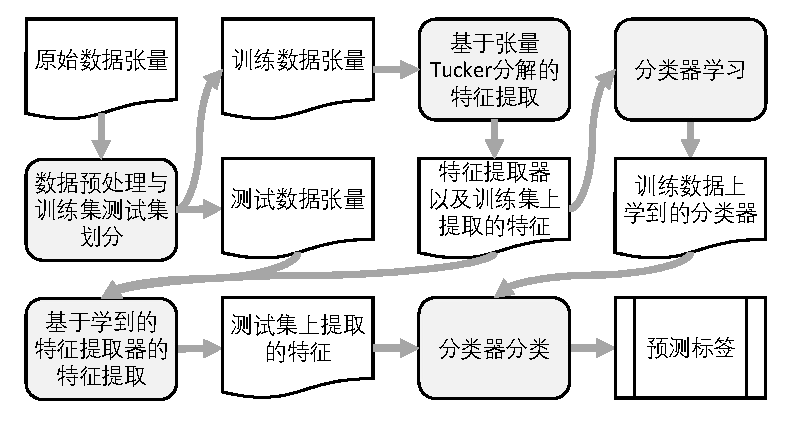
\includegraphics[width=.8\linewidth]{figures/pipeline-ufe.pdf}
	\caption{$\ell_{1}$与$\ell_{\infty}$方法的流程示意图}
	\label{fig:l1linf-routine}
\end{figure}

\section{$\ell_{1}$方法的优化模型与优化算法}
\esection{The Optimization Model and Optimization Algorithm of the $\ell_{1}$ Method}
本节将首先给出$\ell_{1}$方法的优化模型,并分析其利弊。之后,本节将设计一种用于求解$\ell_{1}$方法的有效优化算法,并对该算法进行理论上的收敛性分析以及计算复杂度分析。
\subsection{$\ell_{1}$方法的优化模型}\label{sec:l1}
\esubsection{The Optimization Model of the $\ell_{1}$ Method}
如\refsection{sec:l2}所述,$\ell_2$方法由于目标函数平滑,因此相对容易求解。但是,在实际应用场景中数据往往存在噪声与离群点,而$\ell_2$方法对它们敏感,因而并不鲁棒。这将直接影响到被提取的特征的质量。为了从带噪声与离群点的数据中更加有效地提取特征,受到机器学习理论\ucite{Goodfellow2016}与相关工作的启发,本节提出了基于$\ell_{1}$范数的非负张量Tucker分解方法(简称$\ell_{1}$方法)以提升在噪声场景下的特征提取的鲁棒性。与$\ell_{2}$方法(即\refopt{eq:L2})类似,$\ell_{1}$方法的优化模型为
\begin{equation}\label{eq:L1}
\hspace{1em}
    \begin{aligned}
    &\underset{\mathclap{\{\mathbfcal{G}^{(i)}\}_{i=1}^{n}, \{\boldsymbol{A}^{(j)}\}_{j=1}^{d}}}{\min} \qquad\quad &&\sum_{k=1}^{n}\left\|\mathbfcal{X}^{(k)}-\mathbfcal{G}^{(k)} \times_{1} \boldsymbol{A}^{(1)} \times_{2} \boldsymbol{A}^{(2)} \times_{3} \ldots \times_{d} \boldsymbol{A}^{(d)}\right\|_{F} \\
    &\text{s.t.} && \mathbfcal{G}^{(i)}\in\mathbb{R}_{+}^{r_1 \times r_2 \times \ldots \times r_d},~\forall~i\in[n] ,~\boldsymbol{A}^{(j)}\in \mathbb{R}_{+}^{n_j \times r_j},~\forall~j\in[d],
    \end{aligned}
\end{equation}
其中各符号的意义与\refsection{sec:l2}中相同,这里不再赘述。与$\ell_{2}$方法相异,$\ell_{1}$方法直接计算所有样本Tucker分解拟合误差之和作为其目标函数,因而具备更好的抗噪性能\ucite{Goodfellow2016}。然而,尽管如此,
% 可以在一定程度上抑制数据中的噪声与离群点所带来的负面影响,但其
$\ell_{1}$方法分配给不同样本的权重仍然是相同的,而这正是$\ell_{1}$方法不太合理的地方。直观上来讲,应该更关注于那些具有更大拟合误差的样本,因为一旦控制住了它们的拟合误差,那么最坏情况下的特征提取效用也就得到了保证。此外,由于\refopt{eq:L1}的目标函数是非光滑的,它的求解将会是难题。下一节将设计一种有效的优化算法来求解这个优化难题。

\subsection{优化算法设计}\label{sec:l1-algodesign}
\esubsection{Design of the Optimization Algorithm}
基于迭代优化的思想,本节设计一种用于求解\refopt{eq:L1}的有效迭代优化算法。本节接下来依次推导各个优化变量的更新公式。

\textbf{$\{\mathbfcal{G}^{(i)}\}_{i=1}^{n}$的更新:}固定$i\in[n]$,仅与$\mathbfcal{G}^{(i)}$有关的子问题如下
\begin{equation*}
    \begin{aligned}
    &\underset{\mathclap{\mathbfcal{G}^{(i)}}}{\min} &&\left\|\mathbfcal{X}^{(i)}-\mathbfcal{G}^{(i)} \times_{1} \boldsymbol{A}^{(1)} \times_{2} \boldsymbol{A}^{(2)} \times_{3} \ldots \times_{d} \boldsymbol{A}^{(d)}\right\|_{F} \\
    &\text{s.t.} && \mathbfcal{G}^{(i)}\in\mathbb{R}_{+}^{r_1 \times r_2 \times \ldots \times r_d}.
    \end{aligned}
\end{equation*}
通过简单的平方技巧,上述优化问题等价于如下更容易求解的光滑优化问题
\begin{equation*}
\begin{aligned}
    &\underset{{\mathbfcal{G}^{(i)}}}{\min} && \left\|\mathbfcal{X}^{(i)}-\mathbfcal{G}^{(i)} \times_{1} \boldsymbol{A}^{(1)}\times_{2} \boldsymbol{A}^{(2)}\times_{3}  \ldots \times_{d} \boldsymbol{A}^{(d)}\right\|_{F}^2 \\ &\text{s.t.} && \mathbfcal{G}^{(i)}\in\mathbb{R}_{+}^{r_1 \times r_2 \times \ldots \times r_d}.
\end{aligned}
\end{equation*}
由于以上优化问题对不同的$i=1,2,\ldots,n$均具有相同的形式,因而可以将它们垛叠起来一并分析,即如下优化问题
\begin{equation*}
\begin{aligned}
    &\underset{\mathbfcal{G}}{\min}&& \left\|\mathbfcal{X}-\mathbfcal{G} \times_{1} \boldsymbol{A}^{(1)} \times_{2} \boldsymbol{A}^{(2)}\times_{3} \ldots \times_{d} \boldsymbol{A}^{(d)}\right\|_{F}^2 \\ &\text{s.t.}&& \mathbfcal{G}\in\mathbb{R}_{+}^{r_1 \times r_2 \times \ldots \times r_d \times n},
\end{aligned}
\end{equation*}
其中$\mathbfcal{G}$由$\mathbfcal{G}^{(i)}$垛叠而成。由于该问题是标准的非负张量Tucker分解问题,因此可以直接应用文献\ucite{nnegTucker}中介绍的算法更新之(该算法的本质仍为非负矩阵分解的Lee-Seung算法\ucite{lee2001algorithms}),即
\begin{equation}\label{eq:l1-updateG}
	\mathbfcal{G} \leftarrow \mathbfcal{G} \oast \frac{\mathbfcal{X} \times_{1} {\boldsymbol{A}^{(1)}}^{\top}\times_{2} {\boldsymbol{A}^{(2)}}^{\top}\times_{3}  \ldots \times_{d} {\boldsymbol{A}^{(d)}}^{\top}}
	{\mathbfcal{G} \times_{1} {\boldsymbol{A}^{(1)}}^{\top} \boldsymbol{A}^{(1)} \times_{2} {\boldsymbol{A}^{(2)}}^{\top} \boldsymbol{A}^{(2)} \times_{3}  \ldots \times_{d} {\boldsymbol{A}^{(d)}}^{\top} \boldsymbol{A}^{(d)}}.
\end{equation}
% \ucite{nnegTucker}

\textbf{$\{\boldsymbol{A}^{(j)}\}_{j=1}^{d}$的更新:}固定$j\in[d]$,仅与$\boldsymbol{A}^{(j)}$有关的子问题如下
\begin{equation*}
% \hspace{-0.5em}
\begin{aligned}
    &\underset{\boldsymbol{A}^{(j)}}{\min}\qquad&& \sum_{k=1}^{n}\left\|\mathbfcal{X}^{(k)}-\mathbfcal{G}^{(k)} \times_{1} \boldsymbol{A}^{(1)} \times_{2} \boldsymbol{A}^{(2)}\times_{3}\ldots \times_{d} \boldsymbol{A}^{(d)}\right\|_{F} \\ &\text{s.t. }&& \boldsymbol{A}^{(j)}\in \mathbb{R}_{+}^{n_j \times r_j}.
\end{aligned}
\end{equation*}
利用\refsection{sec:tensor-decomp}中介绍的mode-$j$展开技巧,上述优化问题可以被等价为其矩阵形式,即
\begin{equation}\label{eq:l1-socp}
\begin{aligned}
    &\underset{\boldsymbol{A}^{(j)}}{\min}\qquad&& \sum_{k=1}^{n}\left\|\boldsymbol{X}^{(k)}_{(j)}  - \boldsymbol{A}^{(j)} \boldsymbol{G}^{(k)}_{(j)} {\boldsymbol{A}^{(\setminus j)}}^{\top} \right\|_{F} \\ &\text{s.t. }&& \boldsymbol{A}^{(j)}\in \mathbb{R}_{+}^{n_j \times r_j},
\end{aligned}
\end{equation}
其中
\begin{equation*}
    \boldsymbol{A}^{(\setminus j)} := \boldsymbol{A}^{(d)} \otimes \ldots \otimes \boldsymbol{A}^{(j+1)} \otimes \boldsymbol{A}^{(j-1)} \otimes \ldots \otimes \boldsymbol{A}^{(1)}.
\end{equation*}
更进一步地,以上优化问题可以被再次等价为如下优化问题
\begin{equation*}
    \begin{aligned}
    &\underset{\mathclap{\boldsymbol{A}^{(j)},\boldsymbol{q}}}{\min} && \boldsymbol{q}^{\top}\boldsymbol{1}_{n} \\
    &\text{s.t.} && \left\|\boldsymbol{X}^{(k)}_{(j)}- \boldsymbol{A}^{(j)} \boldsymbol{G}^{(k)}_{(j)} {\boldsymbol{A}^{(\setminus j)}}^{\top}\right\|_{F} \leq q_{k},~\forall~ k\in[n],~\boldsymbol{A}^{(j)} \in \mathbb{R}_{+}^{n_j \times r_j}.
    \end{aligned}
\end{equation*}
变换到这一步时,$\boldsymbol{A}^{(j)}$子问题其实就已经被解决了。这是因为上述优化问题为二阶锥规划问题\ucite{alizadeh2003second},而二阶锥规划为凸优化问题\ucite{boyd2004convex}。这个问题已经在业内被广泛研究与应用,并且已经有许多成熟的凸优化求解器可以快速求解。本文将使用求解器MOSEK\footnote{\url{https://www.mosek.com/}}来求解上述优化问题。

用于求解$\ell_1$方法的优化算法如\refalg{alg:l1}所示。具体来说,\refalg{alg:l1}首先初始化核心张量与因子矩阵(第1行)。之后,\refalg{alg:l1}使用\refequation{eq:l1-updateG}来更新核心张量$\mathbfcal{G}$(第4行),并通过使用MOSEK求解一系列二阶锥规划问题的方式来更新因子矩阵$\{\boldsymbol{A}^{(j)}\}_{j=1}^{d}$(第5-6行)。在达到某些收敛条件时,\refalg{alg:l1}将停止迭代,并返回学习得到的特征提取器$\{\boldsymbol{A}^{(j)}\}_{j=1}^{d}$(第9行)。

\begin{algorithm}[t]\setstretch{1.35}
	\begin{algorithmic}[1]
	\REQUIRE 张量$\mathbfcal{X} \in \mathbb{R}_{+}^{n_1 \times n_2 \times \ldots \times n_d \times n}$、核心张量前$d$维的维度(可由\refalg{alg_re}得到)、最大迭代步数$\Phi$以及MOSEK的求解精度$\epsilon$
	\ENSURE 学习得到的特征提取器
	\STATE 赋$t\leftarrow 0$,并随机初始化$\mathbfcal{G}_{t} \in \mathbb{R}_{+}^{r_1 \times r_2 \times \ldots \times r_d \times n}$和$\boldsymbol{A}^{(j)}_{t}\in \mathbb{R}_{+}^{n_j \times r_j}$,$\forall~ j\in[d]$;\hspace{-2em}
    \WHILE{$t<\Phi$并且算法未收敛}
    \STATE 更新$\mathbfcal{G}_{t+1} \leftarrow \mathbfcal{G}_{t} \oast ((\mathbfcal{X} \times_{1} {\boldsymbol{A}_{t}^{(1)}}^{\top} \times_{2} {\boldsymbol{A}_{t}^{(2)}}^{\top} \times_{3} \ldots \times_{d} {\boldsymbol{A}_{t}^{(d)}}^{\top})\oslash
	(\mathbfcal{G}_{t} \times_{1} {\boldsymbol{A}_{t}^{(1)}}^{\top} \boldsymbol{A}_{t}^{(1)} \times_{2} {\boldsymbol{A}_{t}^{(2)}}^{\top} \boldsymbol{A}_{t}^{(2)} \times_{3}  \ldots \times_{d} {\boldsymbol{A}_{t}^{(d)}}^{\top} \boldsymbol{A}_{t}^{(d)}))$;
    \FOR{$j=1,2,\ldots,d$}
    \STATE 更新$\boldsymbol{A}_{t+1}^{(j)}\leftarrow$使用MOSEK求解如下二阶锥规划问题(直到误差小于$\epsilon$)
    \begin{equation*}
    \boxed{
        \begin{aligned}
        &\underset{\mathclap{\boldsymbol{A}^{(j)},\boldsymbol{q}}}{\min} && \boldsymbol{q}^{\top}\boldsymbol{1}_{n} \\
        &\text{s.t.} && \left\|\boldsymbol{X}^{(k)}_{(j)}- \boldsymbol{A}^{(j)} \left(\boldsymbol{G}_{t+1}^{(k)}\right)_{(j)} {\boldsymbol{A}_{t\rightarrow t+1}^{(\setminus j)}}^{\top}\right\|_{F} \leq q_{k},~\forall~ k\in[n],~\boldsymbol{A}^{(j)} \in \mathbb{R}_{+}^{n_j \times r_j},
        \end{aligned}
    }
    \end{equation*}
    得到的最优解,其中$\boldsymbol{A}_{t\rightarrow t+1}^{(\setminus j)} := \boldsymbol{A}_{t}^{(d)} \otimes \ldots \otimes \boldsymbol{A}_{t}^{(j+1)} \otimes \boldsymbol{A}_{t+1}^{(j-1)} \otimes \ldots \otimes \boldsymbol{A}_{t+1}^{(1)}$;
    \ENDFOR
    \STATE 赋$t\leftarrow t+1$
    \ENDWHILE
	\RETURN 学习得到的特征提取器$\{\boldsymbol{A}_{t}^{(j)}\}_{j=1}^{d}$;
	\end{algorithmic}
	\captionsetup{labelsep=period,font=bf}
	\caption{$\ell_1$方法的优化算法}
	\label{alg:l1}
\end{algorithm}


\subsection{优化算法的收敛性分析}\label{sec:conv}
\esubsection{Convergence Analysis of the Optimization Algorithm}
本节从理论上分析\refalg{alg:l1}的收敛性。为方便起见,$\mathcal{J}(\mathbfcal{G},\boldsymbol{A}^{(1)},\allowbreak\ldots,\allowbreak\boldsymbol{A}^{(d)})$表示\refopt{eq:L1}的目标函数。
\begin{theorem}\kaishu
    $\mathcal{J}(\mathbfcal{G},\boldsymbol{A}^{(1)},\ldots,\boldsymbol{A}^{(d)})$在\refalg{alg:l1}的每一步迭代都是下降的,且最终会收敛到局部极小值点。
\end{theorem}
\begin{proof}
证明由以下三个部分组成:
    \begin{enumerate}[noitemsep]
        \item \textbf{$\mathcal{J}(\mathbfcal{G},\boldsymbol{A}^{(1)},\ldots,\boldsymbol{A}^{(d)})$有下界:}这是显然的,因为目标函数$\mathcal{J}(\mathbfcal{G},\boldsymbol{A}^{(1)},\ldots,\boldsymbol{A}^{(d)})$为一系列张量Frobenius范数之和,故它一定有下界$0$。\vspace{1em}
        \item \textbf{$\mathbfcal{G}$($\{\mathbfcal{G}^{(i)}\}_{i=1}^{n}$)的更新:}由于核心张量$\mathbfcal{G}$的更新公式(即\refequation{eq:l1-updateG})的本质为非负矩阵分解的Lee-Seung算法\ucite{lee2001algorithms},由\reflemma{lemma:lee-desc},可以得出以下结论
        \begin{equation*}
        \label{eq:conv1}
            \mathcal{J}(\mathbfcal{G}_{t+1},\boldsymbol{A}^{(1)}_{t},\ldots,\boldsymbol{A}^{(d)}_{t}) \le \mathcal{J}(\mathbfcal{G}_{t}, \boldsymbol{A}^{(1)}_{t},\ldots,\boldsymbol{A}^{(d)}_{t}).
        \end{equation*}
        \item \textbf{$\{\boldsymbol{A}^{(j)}\}_{j=1}^{d}$的更新:}由于本文是通过求解二阶锥规划问题的方式来更新$\boldsymbol{A}^{(j)}$的,而二阶锥规划是凸优化问题,因此求解器MOSEK可以找到它的全局最优解,即
        \begin{equation*}
            \boldsymbol{A}^{(j)}_{t+1}=\underset{\boldsymbol{A}^{(j)}\in\mathbb{R}_{+}^{n_j \times r_j}}{\arg\min}\Hquad\mathcal{J}(\mathbfcal{G}_{t+1},\allowbreak \boldsymbol{A}^{(1)}_{t+1},\allowbreak \ldots, \allowbreak \boldsymbol{A}^{(j-1)}_{t+1}, \allowbreak \boldsymbol{A}^{(j)}, \allowbreak \boldsymbol{A}^{(j+1)}_{t},\allowbreak \ldots,\allowbreak \boldsymbol{A}^{(d)}_{t}),
        \end{equation*}
        而这意味着
        \begin{equation*}
        \begin{aligned} &\mathcal{J}(\mathbfcal{G}_{t+1},\boldsymbol{A}^{(1)}_{t+1},\ldots,\boldsymbol{A}^{(j-1)}_{t+1},\boldsymbol{A}^{(j)}_{t+1},\boldsymbol{A}^{(j+1)}_{t}, \ldots,\boldsymbol{A}^{(d)}_{t}) \\\le &\mathcal{J}(\mathbfcal{G}_{t+1},\boldsymbol{A}^{(1)}_{t+1},\ldots,\boldsymbol{A}^{(j-1)}_{t+1},\boldsymbol{A}^{(j)}_{t},\boldsymbol{A}^{(j+1)}_{t}, \ldots,\boldsymbol{A}^{(d)}_{t}).
        \end{aligned}
        \end{equation*}
        递归地使用上式,可以得到当所有$\boldsymbol{A}^{(j)}$($j=1,2,\ldots,d$)都被更新完后,有
        \begin{equation*}
        \label{eq:conv2}
            \mathcal{J}(\mathbfcal{G}_{t+1},\boldsymbol{A}^{(1)}_{t+1},\ldots,\boldsymbol{A}^{(d)}_{t+1}) \le \mathcal{J}(\mathbfcal{G}_{t+1},\boldsymbol{A}^{(1)}_{t},\ldots,\boldsymbol{A}^{(d)}_{t}).
        \end{equation*}
    \end{enumerate}
    
    综上所述,可以得到
    \begin{equation*}
        \mathcal{J}(\mathbfcal{G}_{t+1},\boldsymbol{A}^{(1)}_{t+1},\ldots,\boldsymbol{A}^{(d)}_{t+1}) \le \mathcal{J}(\mathbfcal{G}_{t},\boldsymbol{A}^{(1)}_{t},\ldots,\boldsymbol{A}^{(d)}_{t}).
    \end{equation*}
    此外,依据实数的完备性\ucite{rudin1976principles},每个单调有界的实数序列都会收敛,故定理得证。
    % 可以得出结论:$\mathcal{J}(\mathbfcal{G},\boldsymbol{A}^{(1)},\ldots,\boldsymbol{A}^{(d)})$在\refalg{alg:l1}的每一步迭代都是下降的,且最终会收敛到一个局部极小值点。
    % 而这意味着\refopt{eq:Linf}的目标函数在每次迭代中都得到了下降。此外,目标函数又是有下界的。依实数的完备性\ucite{rudin1976principles},单调有界序列一定收敛。因此,$\mathcal{J}(\mathbfcal{G},\boldsymbol{A}^{(1)},\allowbreak\ldots,\allowbreak\boldsymbol{A}^{(d)})$最终会收敛到一个局部极小值点。
\end{proof}\vspace{0.5em}

\subsection{优化算法的计算复杂度分析}
\esubsection{Computational Complexity Analysis of the Optimization Algorithm}
本节分析\refalg{alg:l1}的计算复杂度。
% 请读者回忆起$d$代表张量$\mathbfcal{X}$的阶数,$n$代表张量$\mathbfcal{X}$中数据样本的个数,而$n_{j}$和$r_{j}$分别代表了张量$\mathbfcal{X}$以及核心张量$\mathbfcal{G}$第$j$个mode的维度。
在以下的分析中,假设$r_{j}\ll n_{j}$以及$r_{j}\ll\prod_{1\le i\le d,\,i\neq j}n_{i}$,$\forall~ j=1,2,\ldots,d$(这在现实中往往是成立的)。
\begin{theorem}\label{thm:complexity}\kaishu
给定MOSEK的求解精度$\epsilon$,\refalg{alg:l1}每步迭代的计算复杂度为$\mathcal{O}(d\allowbreak(\prod_{i=1}^{d}{n_i})^{3.5} n^{3.5}\ln(\epsilon^{-1}))$,其中$d$为数据样本的阶数,$n_{i}$为数据样本第$i$维的维度,$\forall~ i=1,2,\ldots,d$,而$n$则为数据样本的数量。
\end{theorem}
\begin{proof}
证明由以下两个部分组成:
\begin{enumerate}
    \item \textbf{$\mathbfcal{G}$($\{\mathbfcal{G}^{(i)}\}_{i=1}^{n}$)的更新:}在求解$\mathbfcal{G}$子问题的过程中包含了许多张量与矩阵的乘法,它们的计算复杂度分析如下:计算${\boldsymbol{A}^{(j)}}^{\top}\boldsymbol{A}^{(j)}$的复杂度为$\mathcal{O}(n_{j}{r}_j^{2})$(其中$j\in[d]$);计算\refequation{eq:l1-updateG}的分子和分母的复杂度分别为$\mathcal{O}(n\sum_{i=1}^{d}\allowbreak(\prod_{j=1}^{i}r_{j})\allowbreak(\prod_{j=i}^{d}n_{j}))$和$\mathcal{O}(n\allowbreak(\prod_{j=1}^{d}r_{j})\allowbreak\sum_{i=1}^{d}r_{i})$。由于$r_{j}\ll n_{j}$,$\forall~j =1,2,\ldots,d$,因此更新$\mathbfcal{G}$的总体计算复杂度为$\mathcal{O}(\sum_{i=1}^{d}n_{i}{r_i}^{2} + n\sum_{i=1}^{d}r_{i}\allowbreak(\prod_{j=1}^{i-1}r_{j})\allowbreak(\prod_{j=i}^{d}n_{j}))$。

    \item \textbf{$\{\boldsymbol{A}^{(j)}\}_{j=1}^{d}$的更新:}为了方便起见,此处$\boldsymbol{\Psi}_{k}$代表$\boldsymbol{I}_{n_{j}}\otimes \boldsymbol{A}^{(\setminus j)}\allowbreak {\boldsymbol{G}^{(k)}_{(j)}}^{\top}$。可以将\refopt{eq:l1-socp}等价为
\begin{equation}\label{eq:reform-socp}
	\begin{aligned}
		&\underset{\mathclap{\operatorname{vec}\left({\boldsymbol{A}^{(j)}}^{\top}\right),\boldsymbol{q}}}{\min} \quad && \boldsymbol{q}^{\top}\boldsymbol{1}_{n}\\
		&\text{s.t.} &&
		\left\|\boldsymbol{\Psi}_{k}\operatorname{vec}\left({\boldsymbol{A}^{(j)}}^{\top}\right)-\operatorname{vec}\left({\boldsymbol{X}^{(k)}_{(j)}}^{\top}\right)\right\|_{2} \le q_{k},~ k\in[n], \\\span&& -\abs{a^{(j)}_{mn}}\leq 0,~\forall~ (m,n)\in[n_{j}]\times[r_{j}].
		\end{aligned}
\end{equation}
以上优化问题为标准的二阶锥规划问题。为了将\refopt{eq:l1-socp}转化为上述形式以便MOSEK求解,需要先计算$\{\boldsymbol{\Psi}_{k}\}_{k=1}^{n}$。由于计算$\boldsymbol{A}^{(\setminus j)}{\boldsymbol{G}^{(k)}_{(j)}}^{\top}$的复杂度为$\mathcal{O}((\prod_{1\le i\le j,\,i\neq j}n_{i})\allowbreak(\prod_{i=1}^{d}r_{i}))$(其中$k=1,2,\ldots,n$),故计算$\{\boldsymbol{\Psi}_{k}\}_{k=1}^{n}$的复杂度为$\mathcal{O}(n(\prod_{1\le i\le d,\,i\neq j}n_{i})\allowbreak(\prod_{i=1}^{d}r_{i}+r_{j}{n_j}^{2}))$。此外,由于上述二阶锥规划问题(即\refopt{eq:reform-socp})一共有$n+n_{j}r_{j}$个二阶锥约束,并且每个二阶锥约束的维度为$\prod_{i=1}^{d}n_{i}+1$或$2$,根据MOSEK用以求解二阶锥规划问题的算法\ucite{andersen2003implementing,socp_complexity},给定MOSEK的求解精度$\epsilon$,更新$\boldsymbol{A}^{(j)}$的计算复杂度为$\mathcal{O}((n(\prod_{i=1}^{d}n_{i}+1)+2n_{j}r_{j})^{3.5}\ln(\epsilon^{-1}))$,即$\mathcal{O}((\prod_{i=1}^{d}n_{i})^{3.5}n^{3.5}\ln(\epsilon^{-1}))$。由于更新$\boldsymbol{A}^{(j)}$的计算复杂度较大,它直接控制住了计算$\{\boldsymbol{\Psi}_{k}\}_{k=1}^{n}$的复杂度。因此更新$\{\boldsymbol{A}^{(j)}\}_{j=1}^{d}$的总体计算复杂度为$\mathcal{O}(d(\prod_{i=1}^{d}n_{i})^{3.5}n^{3.5}\ln(\epsilon^{-1}))$。
\end{enumerate}

综上所述,\refalg{alg:l1}每步迭代的计算复杂度为$\mathcal{O}(d(\prod_{i=1}^{d}n_{i})^{3.5}n^{3.5}\ln(\epsilon^{-1}))$。
\end{proof}\vspace{0.5em}

可以发现,更新核心张量$\mathbfcal{G}$的计算复杂度消失在了总体的计算复杂度中。这是由于更新核心张量$\mathbfcal{G}$的计算复杂度被更新因子矩阵$\{\boldsymbol{A}^{(j)}\}_{j=1}^{d}$的计算复杂度控制住了。

% 具体来讲,对于$\ell_{1}$方法中的核心张量更新子问题,其优化方式与$\ell_{\infty}$方法无异;而对于$\ell_{1}$方法中的因子矩阵更新子问题,我们仍可以将其等价为如下的二阶锥规划问题

% 如果令特征的总数量$\prod_{j=1}^{d}n_{j}=n_{0}$,则\refalg{alg:l1}每步迭代的计算复杂度为$\mathcal{O}(d n_{0}^{3.5}n^{3.5}\ln(\epsilon^{-1}))$。

% 而该问题亦可以使用求解器MOSEK来求解。

\section{$\ell_{\infty}$方法的优化模型与优化算法}
\esection{The Optimization Model and Optimization Algorithm of the $\ell_{\infty}$ Method}
本节将首先给出$\ell_{\infty}$方法的优化模型,并分析其优势所在。之后,本节将设计一种用于求解$\ell_{\infty}$方法的有效优化算法。由于该优化算法与$\ell_{1}$方法的优化算法仅有微小差异,本节仅对其做简要的理论分析。

\subsection{$\ell_{\infty}$方法的优化模型}\label{sec:linf}
\esubsection{The Optimization Model of the $\ell_{\infty}$ Method}
如\refsection{sec:l1}所述的那样,$\ell_{1}$方法(\refopt{eq:L1})虽然可以在一定程度上弥补$\ell_{2}$方法的缺陷,但它忽略了不同样本之间的重要性差异。受到鲁棒优化理论\ucite{ben2009robust}的启发,具有最大拟合误差的样本应该被给予最高的权重,从而保证在最坏情况下的特征提取效用性。基于以上讨论,本文另辟蹊径,提出了以下基于$\ell_\infty$范数的非负张量Tucker分解方法(简称$\ell_\infty$方法),其旨在优化所有样本的Tucker分解拟合误差最大值
\begin{equation}\label{eq:Linf}
\hspace{1em}
\begin{aligned}
    &\underset{\mathclap{\{\mathbfcal{G}^{(i)}\}_{i=1}^{n}, \{\boldsymbol{A}^{(j)}\}_{j=1}^{d}}}{\min} \qquad\quad &&\underset{\mathclap{k\in\{1,2,\ldots,n\}}}{\max}\quad \left\|\mathbfcal{X}^{(k)}-\mathbfcal{G}^{(k)} \times_{1} \boldsymbol{A}^{(1)} \times_{2} \boldsymbol{A}^{(2)}\times_{3} \ldots \times_{d} \boldsymbol{A}^{(d)}\right\|_{F}  \\
    &\text{s.t.} && \mathbfcal{G}^{(i)}\in\mathbb{R}_{+}^{r_1 \times r_2 \times \ldots \times r_d},~\forall~i\in[n] ,~\boldsymbol{A}^{(j)}\in \mathbb{R}_{+}^{n_j \times r_j},~\forall~j\in[d],
\end{aligned}
\end{equation}
其中各符号的意义不再赘述。通过这样的方式,便可以有效地控制住最坏情况下的拟合误差,从而进一步提升特征提取的鲁棒性。然而,由于这个优化问题的目标函数也是非光滑的,它的求解也将会是难题。下一节将设计一种有效的优化算法来求解这个优化难题。

\subsection{优化算法设计}\label{sec:linf-algodesign}
\esubsection{Design of the Optimization Algorithm}
基于迭代优化的思想,本节设计一种用于求解\refopt{eq:Linf}的有效迭代优化算法。本节接下来依次推导各个优化变量的更新公式。

\textbf{$\{\mathbfcal{G}^{(i)}\}_{i=1}^{n}$的更新:}固定$i\in[n]$,仅与$\mathbfcal{G}^{(i)}$有关的子问题如下
\begin{equation*}
    \begin{aligned}
        &\underset{\mathclap{\mathbfcal{G}^{(i)}}}{\min} \quad &&\underset{\mathclap{k\in\{1,2,\ldots,n\}}}{\max}\quad \left\|\mathbfcal{X}^{(k)}-\mathbfcal{G}^{(k)} \times_{1} \boldsymbol{A}^{(1)} \times_{2} \boldsymbol{A}^{(2)}\times_{3} \ldots \times_{d} \boldsymbol{A}^{(d)}\right\|_{F}  \\
        &\text{s.t.} && \mathbfcal{G}^{(i)}\in\mathbb{R}_{+}^{r_1 \times r_2 \times \ldots \times r_d}.
    \end{aligned}
\end{equation*}
如果记$\xi=\max_{k\in\{1,2,\ldots,n\}\setminus\{i\}} \|\mathbfcal{X}^{(k)}-\mathbfcal{G}^{(k)} \times_{1} \boldsymbol{A}^{(1)} \times_{2} \boldsymbol{A}^{(2)}\times_{3} \ldots \times_{d} \boldsymbol{A}^{(d)}\|_{F}$,则$\xi$与$\mathbfcal{G}^{(i)}$无关,并且上述优化问题等价于
\begin{equation*}
    \begin{aligned}
        &\underset{\mathclap{\mathbfcal{G}^{(i)}}}{\min} \quad &&\max\left\{\xi,~\left\|\mathbfcal{X}^{(i)}-\mathbfcal{G}^{(i)} \times_{1} \boldsymbol{A}^{(1)} \times_{2} \boldsymbol{A}^{(2)}\times_{3} \ldots \times_{d} \boldsymbol{A}^{(d)}\right\|_{F}\right\} \\
        &\text{s.t.} && \mathbfcal{G}^{(i)}\in\mathbb{R}_{+}^{r_1 \times r_2 \times \ldots \times r_d}.
    \end{aligned}
\end{equation*}
接下来分类讨论:
\begin{enumerate}[label=\emph{情形\arabic*},leftmargin=2\parindent]
    \item 若$\|\mathbfcal{X}^{(i)}-\mathbfcal{G}^{(i)} \times_{1} \boldsymbol{A}^{(1)} \times_{2} \boldsymbol{A}^{(2)}\times_{3} \ldots \times_{d} \boldsymbol{A}^{(d)}\|_{F}\geq\xi$,则上述优化问题等价于
    \begin{equation*}
        \begin{aligned}
            &\underset{{\mathbfcal{G}^{(i)}}}{\min} && \left\|\mathbfcal{X}^{(i)}-\mathbfcal{G}^{(i)} \times_{1} \boldsymbol{A}^{(1)}\times_{2} \boldsymbol{A}^{(2)}\times_{3}  \ldots \times_{d} \boldsymbol{A}^{(d)}\right\|_{F} \\ &\text{s.t.} && \mathbfcal{G}^{(i)}\in\mathbb{R}_{+}^{r_1 \times r_2 \times \ldots \times r_d},
        \end{aligned}
    \end{equation*}
    而该问题为经典的非负张量Tucker分解问题。
    \item 若$\|\mathbfcal{X}^{(i)}-\mathbfcal{G}^{(i)} \times_{1} \boldsymbol{A}^{(1)} \times_{2} \boldsymbol{A}^{(2)}\times_{3} \ldots \times_{d} \boldsymbol{A}^{(d)}\|_{F}<\xi$,则上述优化问题等价于
    \begin{equation*}
    % \label{opt:opt-const}
        \begin{aligned}
            &\underset{{\mathbfcal{G}^{(i)}}}{\min} && \xi \\ &\text{s.t.} && \mathbfcal{G}^{(i)}\in\mathbb{R}_{+}^{r_1 \times r_2 \times \ldots \times r_d}.
        \end{aligned}
    \end{equation*}
    由于该优化问题的目标函数是常数,因而任意满足可行条件的$\mathbfcal{G}^{(i)}$均为该优化问题的解。
    % \begin{equation}\label{eq:sol-set}
    %     \left\{\mathbfcal{G}^{(i)}\in\mathbb{R}_{+}^{r_1 \times r_2 \times \ldots \times r_d}\mid\|\mathbfcal{X}^{(i)}-\mathbfcal{G}^{(i)} \times_{1} \boldsymbol{A}^{(1)} \times_{2} \boldsymbol{A}^{(2)}\times_{3} \ldots \times_{d} \boldsymbol{A}^{(d)}\|_{F}<\xi\right\}.
    % \end{equation}
    
    % 虽然可以不对$\mathbfcal{G}^{(i)}$做任何更新,但是不妨继续求解以下优化问题
    % \begin{equation*}
    %     \begin{aligned}
    %         &\underset{{\mathbfcal{G}^{(i)}}}{\min} && \left\|\mathbfcal{X}^{(i)}-\mathbfcal{G}^{(i)} \times_{1} \boldsymbol{A}^{(1)}\times_{2} \boldsymbol{A}^{(2)}\times_{3}  \ldots \times_{d} \boldsymbol{A}^{(d)}\right\|_{F} \\ &\text{s.t.} && \mathbfcal{G}^{(i)}\in\mathbb{R}_{+}^{r_1 \times r_2 \times \ldots \times r_d}.
    %     \end{aligned}
    % \end{equation*}
    % 由于该优化问题的非负约束与\refopt{opt:opt-const}中的非负约束一致,因而该问题的解仍然为\refopt{opt:opt-const}的解。而继续求解上述问题将可以把所有的$\mathbfcal{G}^{(i)}$子问题($i=1,2,\ldots,n$)联合起来一并分析,并潜在地降低了下一轮迭代的目标函数,好处多多。
\end{enumerate}

综上所述,无论是哪种情形,$\mathbfcal{G}^{(i)}$子问题都等价于如下优化问题
\begin{equation*}
    \begin{aligned}
        &\underset{{\mathbfcal{G}^{(i)}}}{\min} && \left\|\mathbfcal{X}^{(i)}-\mathbfcal{G}^{(i)} \times_{1} \boldsymbol{A}^{(1)}\times_{2} \boldsymbol{A}^{(2)}\times_{3}  \ldots \times_{d} \boldsymbol{A}^{(d)}\right\|_{F} \\ &\text{s.t.} && \mathbfcal{G}^{(i)}\in\mathbb{R}_{+}^{r_1 \times r_2 \times \ldots \times r_d}.
    \end{aligned}
\end{equation*}
通过简单的平方技巧,上述优化问题等价于如下更容易求解的光滑优化问题
\begin{equation*}
\begin{aligned}
    &\underset{{\mathbfcal{G}^{(i)}}}{\min} && \left\|\mathbfcal{X}^{(i)}-\mathbfcal{G}^{(i)} \times_{1} \boldsymbol{A}^{(1)}\times_{2} \boldsymbol{A}^{(2)}\times_{3}  \ldots \times_{d} \boldsymbol{A}^{(d)}\right\|_{F}^2 \\ &\text{s.t.} && \mathbfcal{G}^{(i)}\in\mathbb{R}_{+}^{r_1 \times r_2 \times \ldots \times r_d}.
\end{aligned}
\end{equation*}
由于以上优化问题对不同的$i=1,2,\ldots,n$均具有相同的形式,因而可以将它们垛叠起来一并分析,即如下优化问题
\begin{equation*}
\begin{aligned}
    &\underset{\mathbfcal{G}}{\min}&& \left\|\mathbfcal{X}-\mathbfcal{G} \times_{1} \boldsymbol{A}^{(1)} \times_{2} \boldsymbol{A}^{(2)}\times_{3} \ldots \times_{d} \boldsymbol{A}^{(d)}\right\|_{F}^2 \\ &\text{s.t.}&& \mathbfcal{G}\in\mathbb{R}_{+}^{r_1 \times r_2 \times \ldots \times r_d \times n},
\end{aligned}
\end{equation*}
其中$\mathbfcal{G}$由$\mathbfcal{G}^{(i)}$垛叠而成。由于该问题是标准的非负张量Tucker分解问题,因此可以再次应用文献\ucite{nnegTucker}中介绍的算法更新之,即
\begin{equation}\label{eq:linf-updateG}
	\mathbfcal{G} \leftarrow \mathbfcal{G} \oast \frac{\mathbfcal{X} \times_{1} {\boldsymbol{A}^{(1)}}^{\top}\times_{2} {\boldsymbol{A}^{(2)}}^{\top}\times_{3}  \ldots \times_{d} {\boldsymbol{A}^{(d)}}^{\top}}
	{\mathbfcal{G} \times_{1} {\boldsymbol{A}^{(1)}}^{\top} \boldsymbol{A}^{(1)} \times_{2} {\boldsymbol{A}^{(2)}}^{\top} \boldsymbol{A}^{(2)} \times_{3}  \ldots \times_{d} {\boldsymbol{A}^{(d)}}^{\top} \boldsymbol{A}^{(d)}}.
\end{equation}
% \ucite{nnegTucker}

% 而该问题与$\ell_{1}$方法中的$\mathbfcal{G}^{(i)}$子问题一致。因此,可以直接使用\refequation{eq:l1-updateG}来更新$\{\mathbfcal{G}^{(i)}\}_{i=1}^{n}$。
% 此外,通过一个简单的平方技巧,上述优化问题等价于如下更容易求解的光滑优化问题
% \begin{equation}\label{eq:subp1}
% \begin{aligned}
%     &\underset{{\mathbfcal{G}^{(i)}}}{\min} && \left\|\mathbfcal{X}^{(k)}-\mathbfcal{G}^{(k)} \times_{1} \boldsymbol{A}^{(1)}\times_{2} \boldsymbol{A}^{(2)}\times_{3}  \ldots \times_{d} \boldsymbol{A}^{(d)}\right\|_{F}^2 \\ &\text{s.t.} && \mathbfcal{G}^{(i)}\in\mathbb{R}_{+}^{r_1 \times r_2 \times \ldots \times r_d}.
% \end{aligned}
% \end{equation}
% % 其中$i=1,2,\ldots,n$。
% % 注意到,与原有的\refopt{eq:Linf}不同,添加在\refopt{eq:subp1}的目标函数中的额外平方不会影响\refopt{eq:subp1}的最优解,但这使优化过程更容易。
% 由于\refopt{eq:subp1}对不同的$i=1,2,\ldots,n$均具有相同的形式,因而我们可以将所有的$\mathbfcal{G}^{(i)}$子问题($i=1,2,\ldots,n$)垛叠起来一并分析,即如下优化问题
% \begin{equation}\label{eq:subp1c}
% \begin{aligned}
%     &\underset{\mathbfcal{G}}{\min}&& \left\|\mathbfcal{X}-\mathbfcal{G} \times_{1} \boldsymbol{A}^{(1)} \times_{2} \boldsymbol{A}^{(2)}\times_{3} \ldots \times_{d} \boldsymbol{A}^{(d)}\right\|_{F}^2 \\ &\text{s.t.}&& \mathbfcal{G}\in\mathbb{R}_{+}^{r_1 \times r_2 \times \ldots \times r_d \times n},
% \end{aligned}
% \end{equation}
% 其中$\mathbfcal{G}$由$\mathbfcal{G}^{(i)}$垛叠而成。由于\refopt{eq:subp1c}是一个标准的非负张量Tucker分解问题,它的更新公式可以直接由文献\ucite{nnegTucker}中介绍的算法得到(该算法的本质仍为非负矩阵分解的Lee-Seung算法),即如下的更新公式
% \begin{equation}\label{eq:updateG}
% 	\mathbfcal{G} \leftarrow \mathbfcal{G} \oast \frac{\mathbfcal{X} \times_{1} {\boldsymbol{A}^{(1)}}^{\top}\times_{2} {\boldsymbol{A}^{(2)}}^{\top}\times_{3}  \ldots \times_{d} {\boldsymbol{A}^{(d)}}^{\top}}
% 	{\mathbfcal{G} \times_{1} {\boldsymbol{A}^{(1)}}^{\top} \boldsymbol{A}^{(1)} \times_{2} {\boldsymbol{A}^{(2)}}^{\top} \boldsymbol{A}^{(2)} \times_{3}  \ldots \times_{d} {\boldsymbol{A}^{(d)}}^{\top} \boldsymbol{A}^{(d)}}.
% \end{equation}
% \ucite{nnegTucker}

\textbf{$\{\boldsymbol{A}^{(j)}\}_{j=1}^{d}$的更新:}固定$j\in[d]$,仅与$\boldsymbol{A}^{(j)}$有关的子问题如下
\begin{equation*}
% \hspace{-0.5em}
\begin{aligned}
    &\underset{\boldsymbol{A}^{(j)}}{\min}\qquad&& \underset{\mathclap{k\in\{1,2,\ldots,n\}}}{\max}\quad \left\|\mathbfcal{X}^{(k)}-\mathbfcal{G}^{(k)} \times_{1} \boldsymbol{A}^{(1)} \times_{2} \boldsymbol{A}^{(2)}\times_{3}\ldots \times_{d} \boldsymbol{A}^{(d)}\right\|_{F} \\ &\text{s.t. }&& \boldsymbol{A}^{(j)}\in \mathbb{R}_{+}^{n_j \times r_j}.
\end{aligned}
\end{equation*}
利用\refsection{sec:tensor-decomp}中介绍的mode-$j$展开技巧,上述优化问题可以被等价为其矩阵形式,即
\begin{equation*}
\begin{aligned}
    &\underset{\boldsymbol{A}^{(j)}}{\min}\qquad&& \underset{\mathclap{k\in\{1,2,\ldots,n\}}}{\max}\quad
	\left\|\boldsymbol{X}^{(k)}_{(j)}  - \boldsymbol{A}^{(j)} \boldsymbol{G}^{(k)}_{(j)} {\boldsymbol{A}^{(\setminus j)}}^{\top} \right\|_{F} \\ &\text{s.t. }&& \boldsymbol{A}^{(j)}\in \mathbb{R}_{+}^{n_j \times r_j}.
\end{aligned}
\end{equation*}
% 其中
% \begin{equation*}
%     \boldsymbol{A}^{(\setminus j)} := \boldsymbol{A}^{(d)} \otimes \ldots \otimes \boldsymbol{A}^{(j+1)} \otimes \boldsymbol{A}^{(j-1)} \otimes \ldots \otimes \boldsymbol{A}^{(1)}.
% \end{equation*}
更进一步地,以上优化问题可以被再次等价为如下优化问题
\begin{equation*}
\begin{aligned}
&\underset{\mathclap{\boldsymbol{A}^{(j)},q}}{\min} && q \\
&\text{s.t.} && \left\|\boldsymbol{X}^{(k)}_{(j)}- \boldsymbol{A}^{(j)} \boldsymbol{G}^{(k)}_{(j)} {\boldsymbol{A}^{(\setminus j)}}^{\top}\right\|_{F} \leq q,~\forall~ k\in[n],~\boldsymbol{A}^{(j)} \in \mathbb{R}_{+}^{n_j \times r_j},
\end{aligned}
\end{equation*}
而该问题仍然为二阶锥规划问题,故可以继续使用MOSEK求解之。

% 变换到这一步时,$\boldsymbol{A}^{(j)}$子问题其实就已经被解决了。这是因为上述优化问题为一个二阶锥规划(Second-Order Cone Programming, SOCP)问题\ucite{alizadeh2003second},其已经在业内被广泛研究与应用,并且已经有许多成熟的凸优化求解器可以快速求解该问题。我们将在本文中使用求解器MOSEK\ucite{mosek}来求解上述优化问题。

\begin{algorithm}[t]\setstretch{1.35}
	\begin{algorithmic}[1]
	\REQUIRE 张量$\mathbfcal{X} \in \mathbb{R}_{+}^{n_1 \times n_2 \times \ldots \times n_d \times n}$、核心张量前$d$维的维度(可由\refalg{alg_re}得到)、最大迭代步数$\Phi$以及MOSEK的求解精度$\epsilon$
	\ENSURE 学习得到的特征提取器
	\STATE 赋$t\leftarrow 0$,并随机初始化$\mathbfcal{G}_{t} \in \mathbb{R}_{+}^{r_1 \times r_2 \times \ldots \times r_d \times n}$和$\boldsymbol{A}^{(j)}_{t}\in \mathbb{R}_{+}^{n_j \times r_j}$,$\forall~ j\in[d]$;\hspace{-2em}
    \WHILE{$t<\Phi$并且算法未收敛}
    \STATE 更新$\mathbfcal{G}_{t+1} \leftarrow \mathbfcal{G}_{t} \oast ((\mathbfcal{X} \times_{1} {\boldsymbol{A}_{t}^{(1)}}^{\top} \times_{2} {\boldsymbol{A}_{t}^{(2)}}^{\top} \times_{3} \ldots \times_{d} {\boldsymbol{A}_{t}^{(d)}}^{\top})\oslash
	(\mathbfcal{G}_{t} \times_{1} {\boldsymbol{A}_{t}^{(1)}}^{\top} \boldsymbol{A}_{t}^{(1)} \times_{2} {\boldsymbol{A}_{t}^{(2)}}^{\top} \boldsymbol{A}_{t}^{(2)} \times_{3}  \ldots \times_{d} {\boldsymbol{A}_{t}^{(d)}}^{\top} \boldsymbol{A}_{t}^{(d)}))$;
    \FOR{$j=1,2,\ldots,d$}
    \STATE 更新$\boldsymbol{A}_{t+1}^{(j)}\leftarrow$使用MOSEK求解如下二阶锥规划问题(直到误差小于$\epsilon$)
    \begin{equation*}
    \boxed{
        \begin{aligned}
        &\underset{\mathclap{\boldsymbol{A}^{(j)},q}}{\min} && q \\
        &\text{s.t.} && \left\|\boldsymbol{X}^{(k)}_{(j)}- \boldsymbol{A}^{(j)} \left(\boldsymbol{G}_{t+1}^{(k)}\right)_{(j)} {\boldsymbol{A}_{t\rightarrow t+1}^{(\setminus j)}}^{\top}\right\|_{F} \leq q,~\forall~ k\in[n],~\boldsymbol{A}^{(j)} \in \mathbb{R}_{+}^{n_j \times r_j},
        \end{aligned}
    }
    \end{equation*}
    得到的最优解,其中$\boldsymbol{A}_{t\rightarrow t+1}^{(\setminus j)} := \boldsymbol{A}_{t}^{(d)} \otimes \ldots \otimes \boldsymbol{A}_{t}^{(j+1)} \otimes \boldsymbol{A}_{t+1}^{(j-1)} \otimes \ldots \otimes \boldsymbol{A}_{t+1}^{(1)}$;
    \ENDFOR
    \STATE 赋$t\leftarrow t+1$
    \ENDWHILE
	\RETURN 学习得到的特征提取器$\{\boldsymbol{A}_{t}^{(j)}\}_{j=1}^{d}$;
	\end{algorithmic}
	\captionsetup{labelsep=period,font=bf}
	\caption{$\ell_\infty$方法的优化算法}
	\label{alg:l-infty}
\end{algorithm}

用于求解$\ell_\infty$方法的优化算法如\refalg{alg:l-infty}所示。具体来说,\refalg{alg:l-infty}首先初始化核心张量与因子矩阵(第1行)。之后,\refalg{alg:l-infty}使用\refequation{eq:linf-updateG}来更新核心张量$\mathbfcal{G}$(第4行),并通过使用MOSEK求解一系列二阶锥规划问题的方式来更新因子矩阵$\{\boldsymbol{A}^{(j)}\}_{j=1}^{d}$(第5-6行)。在达到某些收敛条件时,\refalg{alg:l-infty}将停止迭代,并返回学习得到的特征提取器$\{\boldsymbol{A}^{(j)}\}_{j=1}^{d}$(第9行)。

\subsection{优化算法的收敛性分析与计算复杂度分析}
\esubsection{Convergence and Computational Complexity Analyses of the Optimization Algorithm}
\refalg{alg:l-infty}具有如下的理论保证:
\begin{enumerate}
    \item \textbf{收敛性:}可以推出,$\ell_{\infty}$方法的优化算法的收敛性也可以得到理论保证。这是由于$\ell_{\infty}$方法的优化算法与$\ell_{1}$方法的优化算法相比仅有在求解$\boldsymbol{A}^{(j)}$子问题时存在差异,而在这一步时$\ell_{\infty}$方法仍然在使用MOSEK求解二阶锥规划问题,从而保证了该步更新的最优性与下降性。
    \item \textbf{计算复杂度:}可以推出,$\ell_{\infty}$方法的优化算法的计算复杂度与$\ell_{1}$方法的优化算法的计算复杂度相同。这是由于$\ell_{\infty}$方法的优化算法与$\ell_{1}$方法的优化算法相比在求解$\boldsymbol{A}^{(j)}$子问题时的差异仅体现在二阶锥规划问题的目标函数上,而根据MOSEK用以求解二阶锥规划问题的算法\ucite{andersen2003implementing,socp_complexity},其求解二阶锥规划问题的计算复杂度仅与二阶锥约束的数量与维度有关,因而求解$\ell_{\infty}$方法中的二阶锥规划问题的计算复杂度与求解$\ell_{1}$方法中的二阶锥规划问题的计算复杂度是相同的。
    % 因此,$\ell_{\infty}$方法的优化算法的计算复杂度与$\ell_{1}$方法的优化算法的计算复杂度相同。
\end{enumerate}

% \section{$\ell_{\infty}$方法的优化模型与优化算法}

% \section{\texorpdfstring{$\ell_{\infty}$}{L无穷}方法的优化算法及其理论分析}
% \esection{The Optimization Algorithm for Solving the \texorpdfstring{$\ell_{\infty}$}{L-infinity} Method and Its Theoretical Analysis}

\section{本章小结}
\esection{Summary of the Chapter}
本章介绍了两种基于张量优化的鲁棒无监督特征提取方法——$\ell_{1}$与$\ell_{\infty}$方法。$\ell_{1}$方法采用了机器学习中常用的$\ell_{1}$范数来抑制数据中的噪声与离群点所带来的负面影响,但该方法仍存在一定的内在局限性。为了进一步提升特征提取的鲁棒性,受到鲁棒优化理论的启发,$\ell_{\infty}$方法被很自然地提出。$\ell_{\infty}$方法旨在控制住所有样本之中的最大拟合误差,从而能够更好地在带噪声环境下进行特征提取。此外,本章分别为$\ell_{1}$与$\ell_{\infty}$方法设计了有效优化算法,并进行了理论收敛性分析与计算复杂度分析。
%# -*- coding:utf-8 -*-
\chapter{数值仿真与实验结果分析}\label{chap:exp}
\echapter{Numerical Simulations and Analysis}

本章将通过大量的实验来展示本文所提出方法的优越性及特点。首先介绍实验的相关设置,而后给出实验结果并加以分析。

\section{实验设置}
\esection{Experimental Setups}
本节将分别介绍无监督特征选择与提取任务下的数据集、评价指标与方法、对比方法以及参数设置。在本文中,所有的程序均通过MATLAB R2020b编写。此外,所有的实验均运行在一台配备3.70-GHZ i9-10900K CPU和128-GB主内存的Ubuntu服务器上,并且没有使用GPU。当需要在MATLAB中操作张量时,本文使用MATLAB张量工具箱\footnote{\url{https://www.tensortoolbox.org/}}来进行处理。
% 此外,当我们需要使用求解器来求解二阶锥规划时,我们使用业内领先的求解器MOSEK\ucite{mosek}。

\subsection{无监督特征选择实验设置}\label{sec:expsetup-ufs}
\esubsection{Experimental Setups for Unsupervised Feature Selection}
首先介绍使用到的数据集。本文采用了十个真实世界基准数据集,包括两个目标检测数据集(FashionMNIST\footnote{\url{https://github.com/zalandoresearch/fashion-mnist}}和COIL20\footnote{\label{foot:dengcai}\url{http://www.cad.zju.edu.cn/home/dengcai/Data/data.html}}),五个人脸识别数据集(ORL\,\textsuperscript{\ref{foot:dengcai}}、UMIST\footnote{\label{foot:umist}\url{https://eprints.lincoln.ac.uk/id/eprint/16081/}}、Pixraw10P\footnote{\label{foot:jundongl}\url{https://jundongl.github.io/scikit-feature/datasets.html}}、Orlraws10P\,\textsuperscript{\ref{foot:jundongl}}和JAFFE\footnote{\url{https://zenodo.org/record/3451524}}),以及三个医学图像分类数据集(BreastMNIST\footnote{\label{foot:medmnist}\url{https://medmnist.com/}}、OCTMNIST\,\textsuperscript{\ref{foot:medmnist}}和OrganSMNIST\,\textsuperscript{\ref{foot:medmnist}})。作为预处理,上述数据集中的每幅图像的值均被归一化至$[0,1]$。由于在本任务中没有区分训练集与测试集,因而不需要对数据集进行进一步的划分。这些数据集的统计信息如\reftab{tab:datesets-ufs}所示。

\begin{table}[!t]
\centering
\caption{十个用于无监督特征选择的真实世界基准数据集的统计信息}
\label{tab:datesets-ufs}
\begin{tabular}{lrrrr}
\toprule
数据集名称 & 样本数 & 特征尺寸 & 类别数 & 被选择的特征数量区间 \\ \midrule
FashionMNIST  & $1$,$000$          & $28$ $\times$ $28$         & $10$            & $[50,100,150,\ldots,300]$            \\
COIL20  & $1$,$440$          & $32$ $\times$ $32$         & $20$            & $[50,100,150,\ldots,300]$            \\
ORL  & $400$          & $32$ $\times$ $32$         & $40$            & $[50,100,150,\ldots,300]$            \\
UMIST  & $575$          & $23$ $\times$ $28$         & $20$            & $[50,100,150,\ldots,300]$            \\
Pixraw10P     & $100$           & $100$ $\times$ $100$         & $10$            & $[50,100,150,\ldots,300]$             \\
Orlraws10P    & $100$           & $92$ $\times$ $112$         & $10$            & $[50,100,150,\ldots,300]$            \\
BreastMNIST  & $288$          & $28$ $\times$ $28$         & $2$            & $[50,100,150,\ldots,300]$            \\
OCTMNIST      & $400$          & $28$ $\times$ $28$         & $4$            & $[50,100,150,\ldots,300]$  \\
OrganSMNIST    & $220$          & $28$ $\times$ $28$         & $11$            & $[50,100,150,\ldots,300]$            \\
JAFFE    & $213$          & $64$ $\times$ $64$         & $10$            & $[50,100,150,\ldots,300]$            \\
\bottomrule
\end{tabular}

\end{table}

接下来介绍评价指标与方法。在本任务中,由于没有区分训练集与测试集,因而直接在整个数据集上应用不同的方法来选择特征。在特征选择完成之后,通过在被选择特征上的$k$-means聚类\ucite{李航2012统计学习方法}性能来评估被选择特征的质量。本文采用两种被广泛使用的评价指标归一化的互信息(Normalized Mutual Information, NMI)和准确率(Accuracy, ACC)\ucite{cai2010graph}来评估$k$-means聚类的性能。NMI与ACC越高,代表$k$-means聚类的性能越好,因而表示被选择特征的质量越高,也就代表特征选择方法的性能越强。由于$k$-means聚类的结果部分取决于其初始化,因而采用以下策略来缓解评价系统中内在的随机性:对于任意一组被选择的特征,将$k$-means聚类重复运行$20$次并记录平均结果及标准差。

设$n$为样本的总数,$l_i$为第$i$个样本的真实标签,$r_i$为第$i$个样本的聚类标签,并令$\boldsymbol{l}=[l_{1},l_{2},\ldots,l_{n}]$,$\boldsymbol{r}=[r_{1},r_{2},\ldots,r_{n}]$,则NMI与ACC的定义如下
\begin{equation*}
\text{NMI}(\boldsymbol{l}, \boldsymbol{r})=\frac{\operatorname{I}(\boldsymbol{l}, \boldsymbol{r})}{\sqrt{\operatorname{H}(\boldsymbol{l}) \operatorname{H}(\boldsymbol{r})}},
\end{equation*}
\begin{equation*}
    \text {ACC}(\boldsymbol{l}, \boldsymbol{r}) = \frac {1} { n } \sum _ { i = 1 } ^ { n } \delta \left( l _ { i }, \operatorname { map } \left( r _ { i } \right) \right) ,
\end{equation*}
其中$\operatorname{I}(\boldsymbol{l},\boldsymbol{r})$、$\operatorname{H}(\boldsymbol{l})$以及$\operatorname{H}(\boldsymbol{r})$分别为$\boldsymbol{l}$与$\boldsymbol{r}$之间的互信息以及$\boldsymbol{l}$与$\boldsymbol{r}$各自的边际熵\ucite{cover1999elements},而$\operatorname{map}(\cdot)$则为基于匈牙利算法\ucite{kuhn1955hungarian}的最佳排列映射。

最后介绍对比方法与参数设置。为了验证CPUFS与CPUFSnn方法的有效性\footnote{CPUFS与CPUFSnn方法已开源于\url{https://github.com/Kwan1997/CPUFS}},本文将它们与九种前沿的无监督特征选择方法进行比较
% \footnote{本文不会与GRLTR这一基于张量优化的无监督特征选择方法对比,因为它是一种嵌入式特征选择方法,而这超出了本文的范围(本文关注于过滤式特征选择)。}
,包括LapScore\ucite{lapscore}、MCFS\ucite{cai2010unsupervised}、UDFS\ucite{udfs}、SOCFS\ucite{socfs}、SOGFS\ucite{sogfs}、RUFS\ucite{rufs}、RSFS\ucite{rsfs}、 JELSR\ucite{jelsr}以及CDLFS\ucite{cdlfs}。这些方法的详细描述可以在\refsection{sec:review-ufs}中找到。SOGFS的代码由本文作者自行编写实现,而其它所有方法的代码均由其作者提供。此外,还采用仅选择所有原始特征的基线方法AllFea来说明特征选择的效用性所在。本文通过网格搜索策略在$\{10^{-2},10^{-1},1,\allowbreak 10,\allowbreak 10^{2}\}$内调整所有方法的参数。对于CPUFS方法,在所有数据集上均设置$\eta=10^{5}$;对于CPUFSnn方法,在OCTMNIST以及OrganSMNIST数据集上设置$\eta=10^{4}$,而在除这两个数据集以外的所有数据集上均设置$\eta=10^{5}$。对于使用到加权$k$近邻图的方法,设置近邻的数量$k=5$以及高斯核宽度$\sigma=1$。对于基于投影的方法,将投影子空间的维度设置为数据中的类别数的真值$c$;对于基于聚类的方法,也将潜在类别的数量设置为数据中的类别数的真值$c$。此外,设置$\Phi_{1}=500$和$\Phi_{2}=2$。对于每种不同的方法,本文展示其在所有参数组合下的最佳效果。


\subsection{无监督特征提取实验设置}\label{sec:expsetup-ufe}
\esubsection{Experimental Setups for Unsupervised Feature Extraction}

\begin{table}[!t]
	\caption{三个用于无监督特征提取的真实世界基准数据集的统计信息}
	\label{tab:datesets-ufe}
	\centering
% 	\begin{tabular}{lrrr}
% \toprule
% 数据集名称              & COIL20           & Yale           & UMIST          \\ \midrule
% 样本数              & 1,440           & 165            & 565            \\
% 特征尺寸           & $32 \times 32$ & $32 \times 32$ & $32 \times 32$ \\
% 类别数              & 20             & 15             & 20             \\
% 训练集规模 & $32 \times 32 \times 160$ & $32 \times 32 \times 120$ & $32 \times 32 \times 150$ \\
% 测试集规模     & $32 \times 32 \times 1,280$ & $32 \times 32 \times 45$ & $32 \times 32 \times 415$ \\ \bottomrule
% \end{tabular}%
\begin{tabular}{@{}lrrrrr@{}}
\toprule
数据集名称  & 样本数   & 特征尺寸           & 类别数 & 训练集规模                     & 测试集规模                       \\ \midrule
COIL20 & 1,440 & $32 \times 32$ & 20  & $32 \times 32 \times 160$ & $32 \times 32 \times 1,280$ \\
Yale   & 165   & $32 \times 32$ & 15  & $32 \times 32 \times 120$ & $32 \times 32 \times 45$    \\
UMIST  & 565   & $32 \times 32$ & 20  & $32 \times 32 \times 150$ & $32 \times 32 \times 415$   \\ \bottomrule
\end{tabular}%

\end{table}

首先介绍使用到的数据集。本文采用了三个真实世界基准数据集,包括一个目标检测数据集(COIL20\,\textsuperscript{\ref{foot:dengcai}}),两个人脸识别数据集(Yale\,\textsuperscript{\ref{foot:dengcai}}以及UMIST\,\textsuperscript{\ref{foot:umist}})。作为预处理,上述数据集中的每幅图像均被下采样至$32 \times 32$,并且它们的值均被归一化至$[0,1]$。由于在本任务中区分了训练集与测试集,因此需要对数据集进行进一步的划分。这些数据集的具体划分结果以及它们的统计信息如\reftab{tab:datesets-ufe}所示。此外,由于$\ell_{1}$与$\ell_{\infty}$方法旨在抑制数据中的噪声与离群点所带来的负面影响,因而本节还为这三个数据集设计了大量的噪声场景。首先介绍这些噪声的类型。具体而言,为COIL20数据集设计了四种类型的噪声:
\begin{enumerate}
    \item {\boldmath\bfseries ms-$n_{1}\text{-}n_{2}\text{-}n_{3}$:}在训练集的每八张图片中,前三张分别有$n_{1}\%$、$n_{2}\%$以及$n_{3}\%$的像素被随机移除;
    \item {\boldmath\bfseries ms-$n_{1}\text{-}n_{2}\text{-}n_{3}\text{-}n_{4}$:}在训练集的每八张图片中,前四张分别有$n_{1}\%$、$n_{2}\%$、$n_{3}\%$以及$n_{4}\%$的像素被随机移除;
    \item {\boldmath\bfseries sp-$n_{1}\text{-}n_{2}\text{-}n_{3}$:}在训练集的每八张图片中,前三张分别受到密度为$n_{1}\%$、$n_{2}\%$以及$n_{3}\%$的椒盐型噪声污染;
    \item {\boldmath\bfseries sp-$n_{1}\text{-}n_{2}\text{-}n_{3}\text{-}n_{4}$:}在训练集的每八张图片中,前四张分别受到密度为$n_{1}\%$、$n_{2}\%$、$n_{3}\%$以及$n_{4}\%$的椒盐型噪声污染。
\end{enumerate}
为Yale数据集设计了两种类型的噪声:
\begin{enumerate}
    \item {\boldmath\bfseries ms-$n_{1}\text{-}n_{2}\text{-}n_{3}$:}在训练集的每八张图片中,前六张分别有$n_{1}\%$、$n_{1}\%$、$n_{2}\%$、$n_{2}\%$、$n_{3}\%$以及$n_{3}\%$的像素被随机移除;
    \item {\boldmath\bfseries sp-$n_{1}\text{-}n_{2}\text{-}n_{3}$:}在训练集的每八张图片中,前六张分别分别受到密度为$n_{1}\%$、$n_{1}\%$、$n_{2}\%$、$n_{2}\%$、$n_{3}\%$以及$n_{3}\%$的椒盐型噪声污染。
\end{enumerate}
为UMIST数据集设计了两种类型的噪声:
\begin{enumerate}
    \item {\boldmath\bfseries ms-$n_{1}\text{-}n_{2}\text{-}n_{3}$:}在训练集中被随机选择的45张图像中,分别有25、15以及5张图像各自有$n_{1}\%$、$n_{2}\%$以及$n_{3}\%$的像素被随机移除;
    \item {\boldmath\bfseries sp-$n_{1}\text{-}n_{2}\text{-}n_{3}$:}在训练集中被随机选择的45张图像中,分别有25、15以及5张图像分别受到密度为$n_{1}\%$、$n_{2}\%$以及$n_{3}\%$的椒盐型噪声污染。
\end{enumerate}
基于如上设计的噪声类型,生成了如下的噪声场景:
\begin{enumerate}
    \item 在COIL20数据集上,一共生成了34种噪声场景,如\reftab{tab:coil}所示;
    % as shown in \reffig{fig:corr-coil},
    \item 在Yale数据集上,一共生成了18种噪声场景,如\reftab{tab:yale}所示;
    % as shown in \reffig{fig:corr-yale}.
    \item 在UMIST数据集上,一共生成了18种噪声场景,如\reftab{tab:umist}所示。
    % as shown in \reffig{fig:corr-umist}, and
\end{enumerate}
% 本文在附录\refsection{sec:noise-comp}中给出了每一种生成的噪声的示例,以供读者有一个直观的认识。这些生成的噪声图像将用于随后的实验中。

接下来介绍评价指标与方法。由于在本任务中区分了训练集与测试集,因而首先在训练集中应用不同的方法学习得到特征提取器(例如在$\ell_{\infty}$方法中即为$\{\boldsymbol{A}^{(j)}\}_{j=1}^{d}$),而后在测试集上应用学习得到的特征提取器进行特征提取。在特征提取完成之后,通过在被提取特征上的$k$近邻($k$-Nearest Neighbour, KNN)分类性能以及支持向量机(Support Vector Machine, SVM)分类性能来评估被提取特征的质量。本文采用被广泛使用的评价指标ACC\ucite{cai2010graph}来评估分类的性能。(此处的ACC与无监督特征选择任务中的ACC是基本一致的。唯一不同之处在于,由于在本任务中采用分类策略来评估特征提取的质量,因而不再需要匈牙利算法来实现最佳排列(或认为$\operatorname{map}(\cdot)$=$\operatorname{id}(\cdot)$,恒同映射)。故此处不再赘述其具体数学表达式。)ACC越高,代表分类器的性能越好,因而表示被提取特征的质量越高,也就代表特征提取方法的性能越强。

最后介绍对比方法与参数设置。为了验证$\ell_{1}$与$\ell_{\infty}$方法的有效性\footnote{$\ell_{1}$与$\ell_{\infty}$方法已开源于\url{https://github.com/Kwan1997/Linf}},本文将其与$\ell_{2}$方法以及其它六种经典的无监督特征提取方法进行比较,包括概率主成分分析方法(Probabilistic PCA, ProbPCA)\ucite{ProbPCA}、因子分析方法(Factor Analysis, FA)\ucite{FA}、保距映射方法(Isometric Mapping, IsoMap)\ucite{IsoMap}、局部线性嵌入方法(Locally Linear Embedding, LLE)\ucite{LLE}、拉普拉斯特征图方法(Laplacian Eigenmaps, LapE)\ucite{LapE} 以及自编码器方法(Autoencoder, AE)\ucite{Goodfellow2016}。对于这六种经典无监督特征提取方法,它们的代码均由Matlab降维工具箱\footnote{\url{https://lvdmaaten.github.io/drtoolbox/}}提供。此外,由于这六种经典方法是基于矩阵优化的,因而在应用它们时会将数据向量化。由于$\ell_{1}$、$\ell_{2}$以及$\ell_{\infty}$方法并没有内置参数,因此无需对其进行参数调整。对于IsoMap、LLE和LapE,设置其$k$近邻图的$k=20$。此外,由于这三种方法不支持精确的样本外映射,故使用了Nystr{\"o}m逼近算法\ucite{farahat2011novel}来从测试集中提取特征。对于AE,将其全连接层尺寸设置为$f_{0}\shortrightarrow \ceil{1.2f_{0}}+5\shortrightarrow \ceil{f_{0}/4}+3\shortrightarrow \ceil{f_{0}/10}\shortrightarrow f$,其中$f_{0}$表示原始特征的数量(在本文中,对于所有数据集而言均为$32\times 32=1,024$),而$\ceil{\cdot}$是向上取整函数。此外,通过三折交叉验证以及参数网格搜索策略来调整两个分类器的参数。具体来讲,在搜索空间$\{1,2,\ldots,10\}$中为$k$近邻分类器的$k$参数进行调整,以及在搜索空间$\{2^{i}\}_{i=-7}^{7}$中为支持向量机分类器的两个参数进行调整。对于每种不同的方法,本文展示其在所有参数组合下的最佳效果。
% 它的定义为
% \begin{equation*}
%     \ceil{x}=\min \{n \in \mathbb{Z} \mid n \geq x\}.
% \end{equation*}


% \subsection{实验环境设置与数据集介绍}\label{sec:dataset}
% \esubsection{Environmental Settings and Dataset Introduction}

% % \subsection{数据集}\label{sec:dataset}
% % \esubsection{Datasets}

% \subsection{评价指标与评价方法}
% \esubsection{Evaluation Metrics and Evaluation Methodology}

% \subsection{对比方法与参数设置}\label{sec:comp-methods}
% \esubsection{Comparative Methods and Parameter Settings}

\section{无监督特征选择实验}
\esection{Experiments on Unsupervised Feature Selection}
本节将展示无监督特征选择任务的实验结果,并加以分析。
\begin{sidewaysfigure}
    \centering
    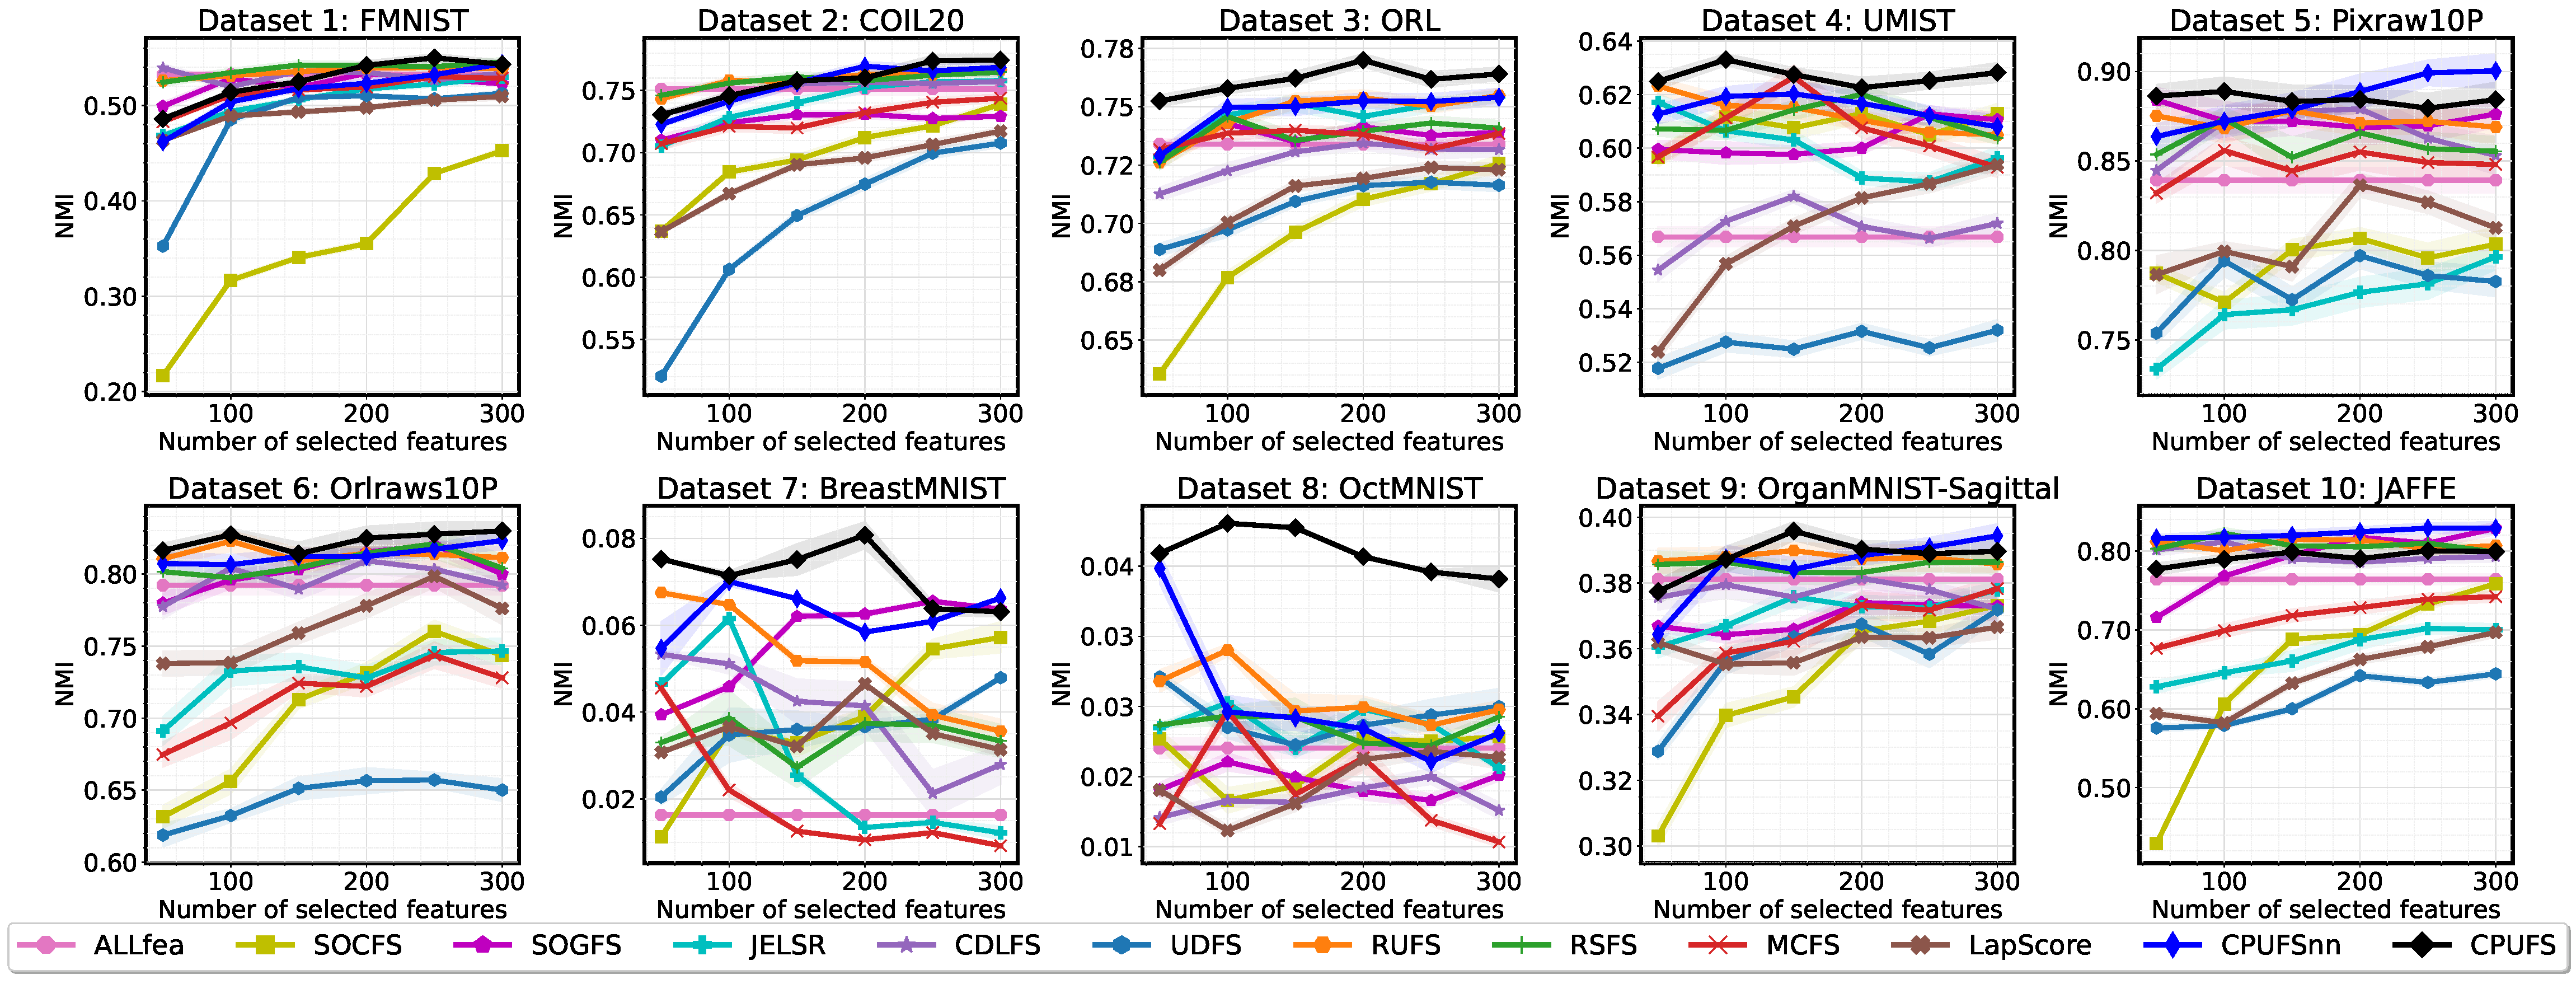
\includegraphics[width=\linewidth]{figures/CPUFS/NMIACC/PAMI_NMI.pdf}
    \caption{不同的无监督特征选择方法在十个数据集上的NMI效果对比}
    \label{fig:clusnmi}
\end{sidewaysfigure}

\begin{sidewaysfigure}
    \centering
    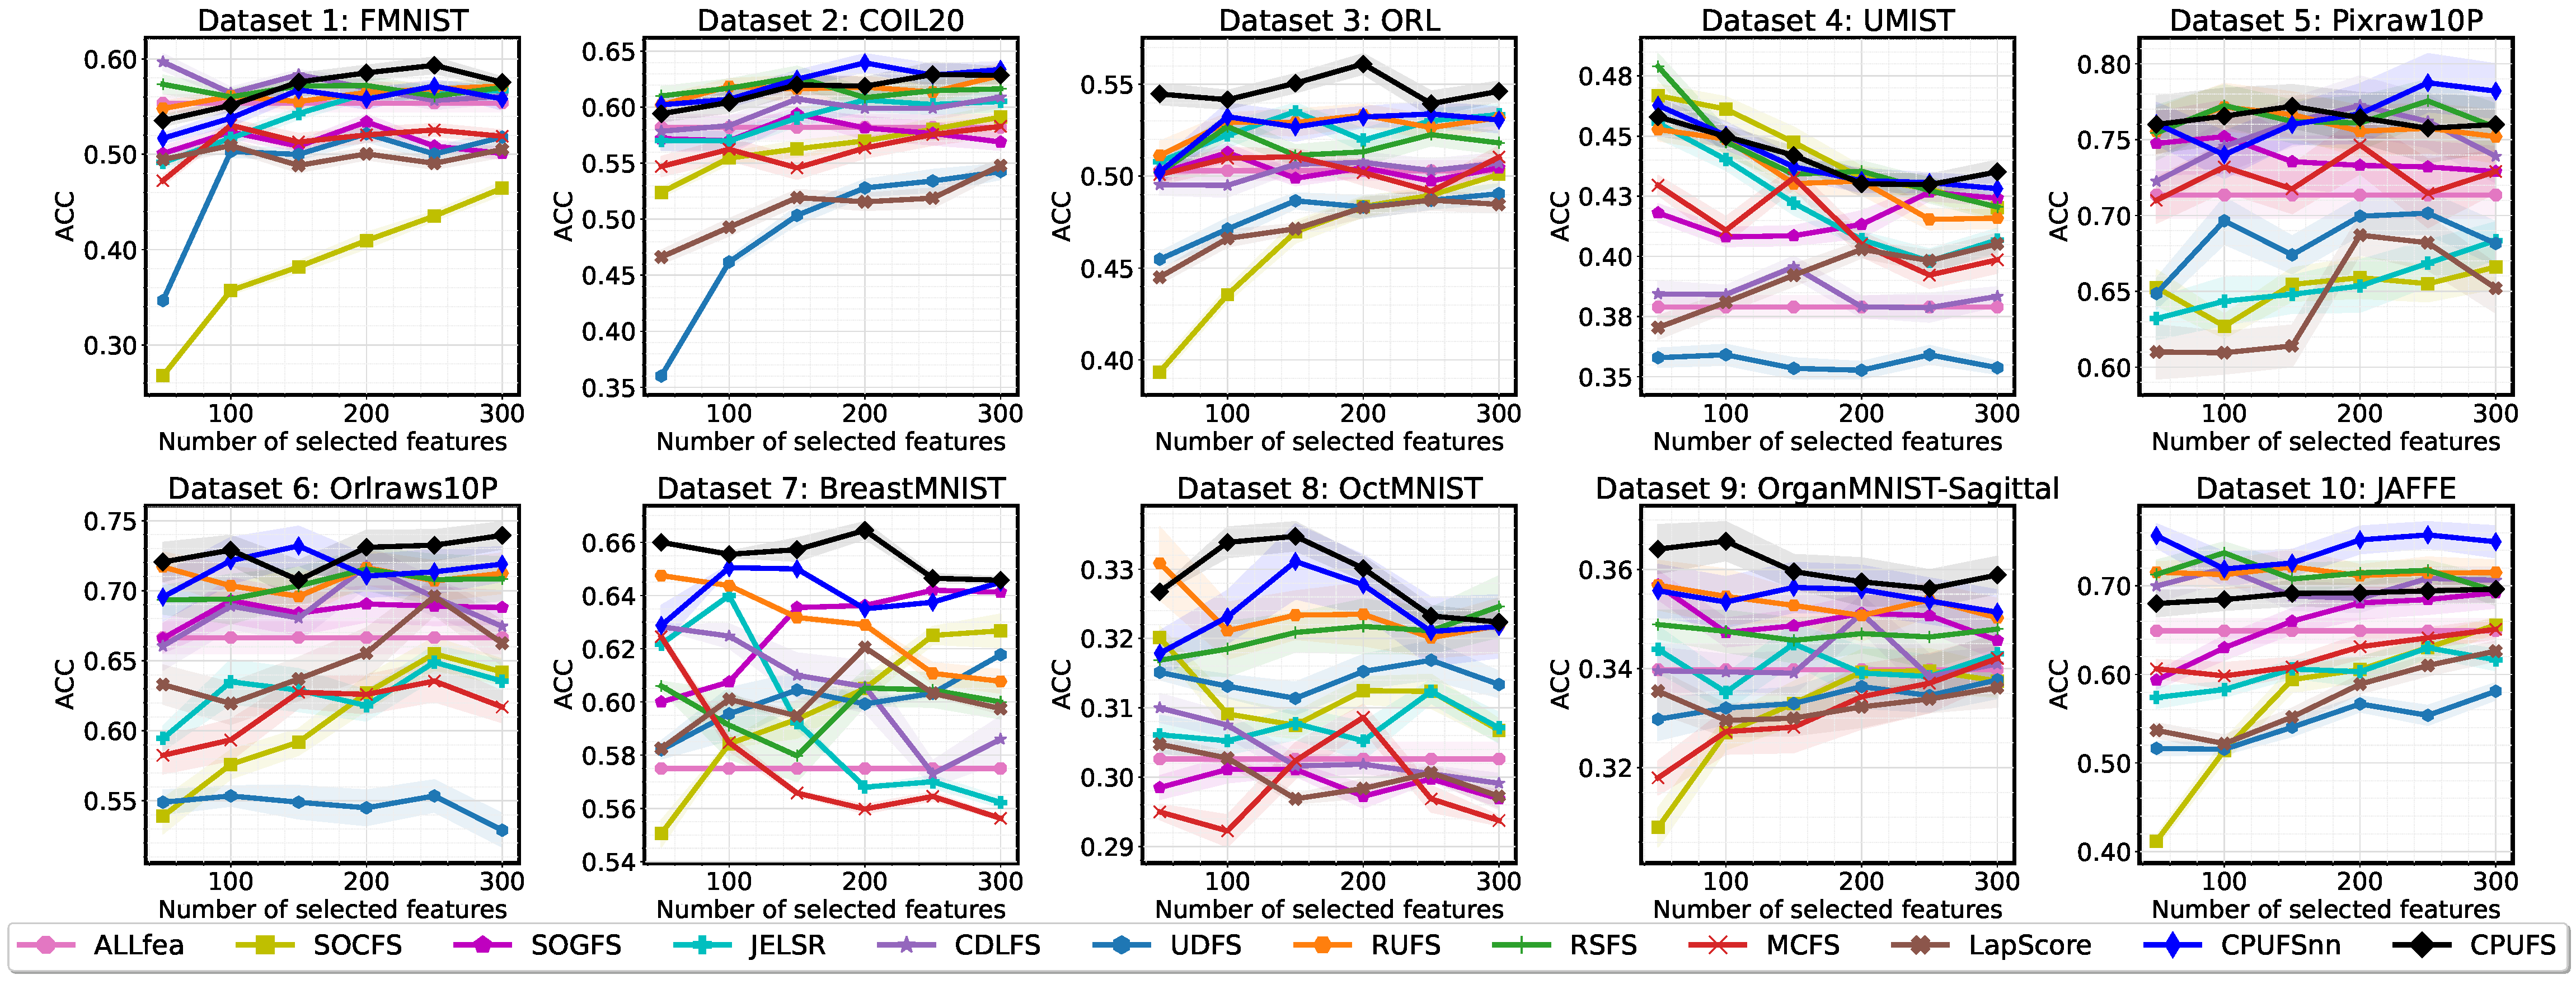
\includegraphics[width=\linewidth]{figures/CPUFS/NMIACC/PAMI_ACC.pdf}
    \caption{不同的无监督特征选择方法在十个数据集上的ACC效果对比}
    \label{fig:clusacc}
\end{sidewaysfigure}

% \subsection{实验一:CPUFS与CPUFSnn和前沿无监督特征选择方法的性能对比}
% \esubsection{Experiment 1: Performance Comparison of the CPUFS and CPUFSnn Methods against the State-of-the-Arts}
\subsection{性能对比}
\esubsection{Performance Comparison}
本节通过比较在被选择特征上的聚类性能来评估不同无监督特征选择方法的性能。
具体来讲,首先分别使用不同的无监督特征选择方法在\refsection{sec:expsetup-ufs}中所提及的所有数据集中进行特征选择,然后基于被选择的特征使用$k$-means聚类算法进行聚类,并依据聚类互信息与准确率来评估不同特征选择方法的性能。
实验结果如\reffig{fig:clusnmi}和\reffig{fig:clusacc}所示,其中阴影区域代表区间$[\mu-0.2\sigma,\mu+0.2\sigma]$(其中$\mu$和$\sigma$分别代表$20$次$k$-means聚类实验的平均值和标准差)。为了方便凸显本文提出的方法,使用具有更大菱形标记的黑色折线代表CPUFS方法,而使用具有较小菱形标记的深蓝色折线代表CPUFSnn方法。基于\reffig{fig:clusnmi}和\reffig{fig:clusacc},可以得出以下结论:
\begin{enumerate}
    \item \textbf{特征选择可提高数据质量:}
    与基线方法ALLfea相比,几乎所有无监督特征选择方法均具有更强的$k$-means聚类性能。这表明特征选择确实可以过滤数据中的冗余和嘈杂特征,因此具有非常重要的作用。
    \item \textbf{CPUFS和CPUFSnn方法在性能上超过了前沿方法:}
    就可达到的最大NMI而言,在这十个数据集之中的任意一个上,总有CPUFS与CPUFSnn中的一个方法是最优的,并且有时CPUFS与CPUFSnn同时包揽前二。虽然在最大可达的ACC方面,CPUFS与CPUFSnn方法并不总是最好的,但在除了FashionMNIST和UMIST之外的所有数据集上,它们之中至少有一个方法仍然可以优于所有对比方法。这充分说明了CPUFS和CPUFSnn方法的有效性。
    % 这主要归因于CPUFS和CPUFSnn方法完好地保留了张量的结构信息。
    \item \textbf{CPUFS和CPUFSnn方法分别适用于不同的场合:}从\reffig{fig:clusnmi}和\reffig{fig:clusacc}中不难发现,其实很难确定究竟是CPUFS方法更好还是CPUFSnn方法更好。例如,在JAFFE数据集上,CPUFSnn方法会达到比CPUFS方法更好的性能;而在ORL数据集上,CPUFSnn方法却表现地比CPUFS方法更差。这个现象表明,线性分类器的非负性并不总是有利于特征选择,但在某些情况下,它确实提升了被选择特征的质量。因此需要因地制宜地确定是否该对线性分类器施加非负约束。
    \item \textbf{“天下没有免费的午餐”\ucite{wolpert1997no}:}可以从\reffig{fig:clusnmi}和\reffig{fig:clusacc}中观察到,没有一种无监督特征选择方法可以在所有数据集上均达到最优,并且不同的方法最适用于不同的数据集。 例如,就ACC而言,SOCFS在FashionMNIST数据集上表现地最差,然而在UMIST数据集上,它又表现地相当之好。尽管如此,值得注意的是,CPUFS和CPUFSnn方法可以较为稳定地在几乎所有数据集上就所有评价指标而言均有优秀的性能。这凸显了它们的稳健性和有效性。
\end{enumerate}

\begin{figure}[!t]
    \centering
    % \subfloat[null]{
\includegraphics[width=0.33\linewidth]{figures/CPUFS/visualization/feaOriginal_ORL.pdf}}
    % \subfloat[null]{
\includegraphics[width=0.33\linewidth]{figures/CPUFS/visualization/feaOriginal_ORL.pdf}}
    % \subfloat[null]{
\includegraphics[width=0.33\linewidth]{figures/CPUFS/visualization/feaOriginal_ORL.pdf}}\\
    % \subfloat[null]{
\includegraphics[width=0.33\linewidth]{figures/CPUFS/visualization/feaOriginal_ORL.pdf}}
    % \subfloat[null]{
\includegraphics[width=0.33\linewidth]{figures/CPUFS/visualization/feaOriginal_ORL.pdf}}
    % \subfloat[null]{
\includegraphics[width=0.33\linewidth]{figures/CPUFS/visualization/feaOriginal_ORL.pdf}}
    \subfloat[FashionMNIST ($\nu$)\label{fig:f1}] {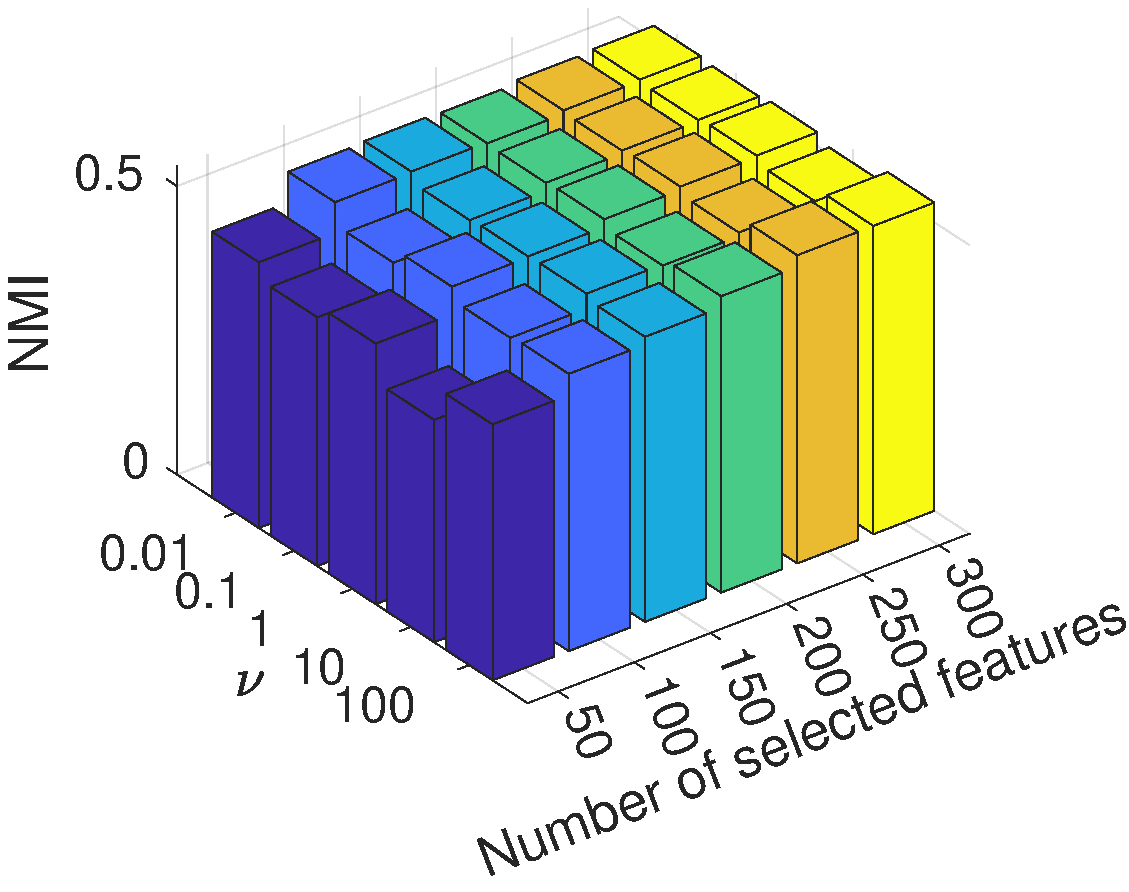
\includegraphics[width=0.33\linewidth]{figures/CPUFS/sensitivity/fmnist_nu.pdf}}
    \subfloat[FashionMNIST ($\alpha$)\label{fig:f2}]{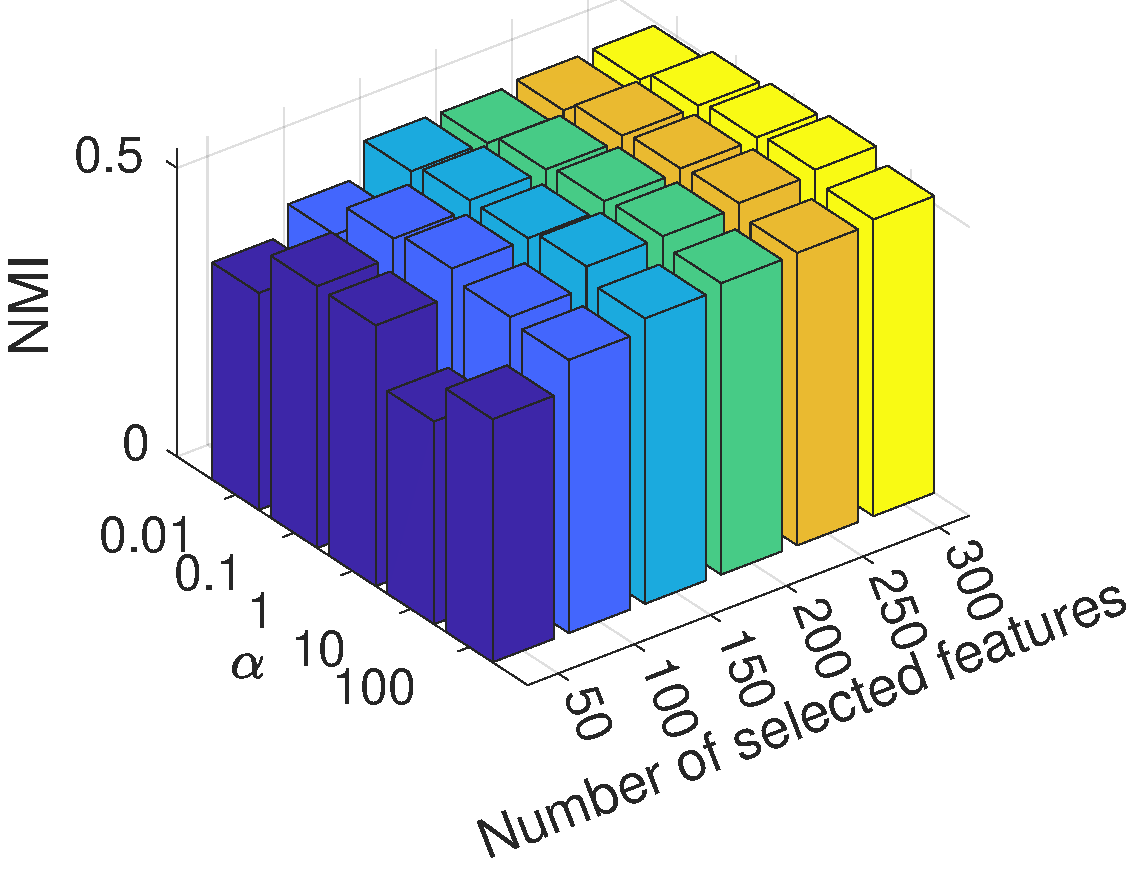
\includegraphics[width=0.33\linewidth]{figures/CPUFS/sensitivity/fmnist_alpha.pdf}}
    \subfloat[FashionMNIST ($\beta$)\label{fig:f3}]{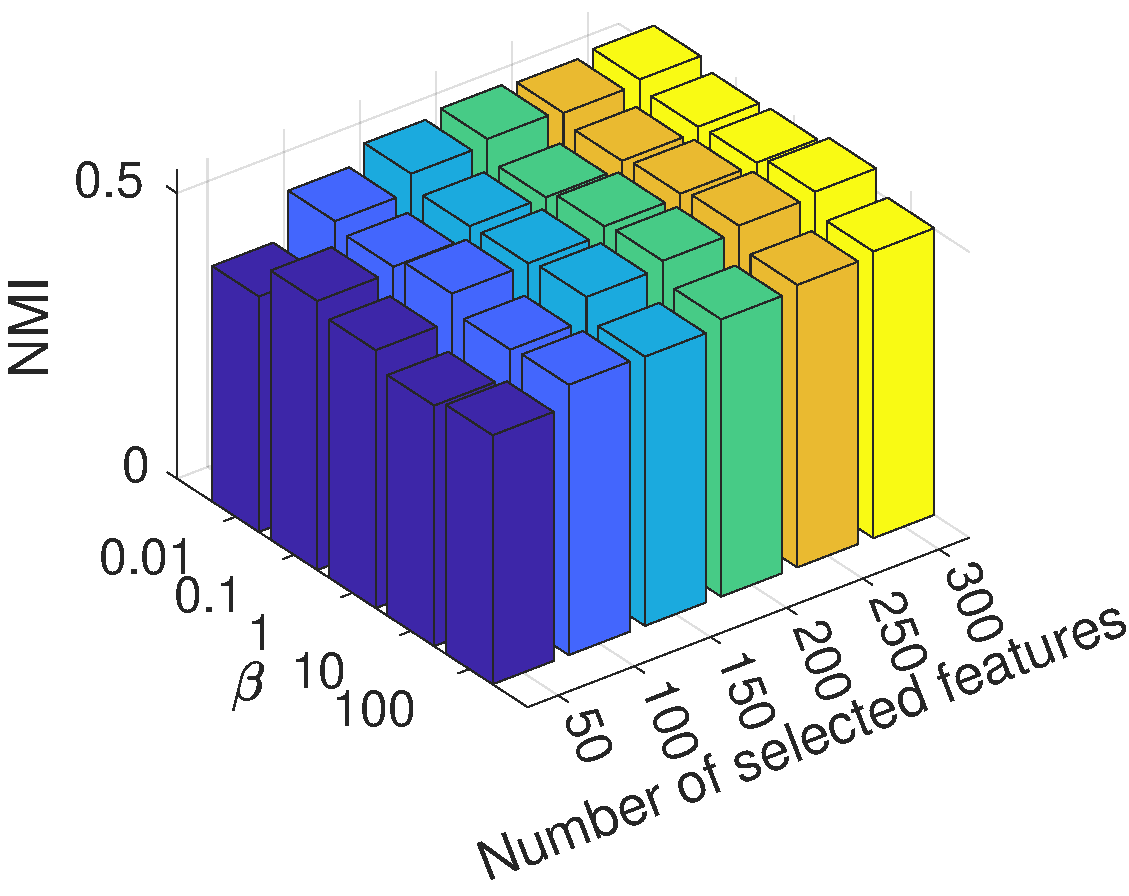
\includegraphics[width=0.33\linewidth]{figures/CPUFS/sensitivity/fmnist_beta.pdf}}\\
    \subfloat[COIL20 ($\nu$)\label{fig:l1}] {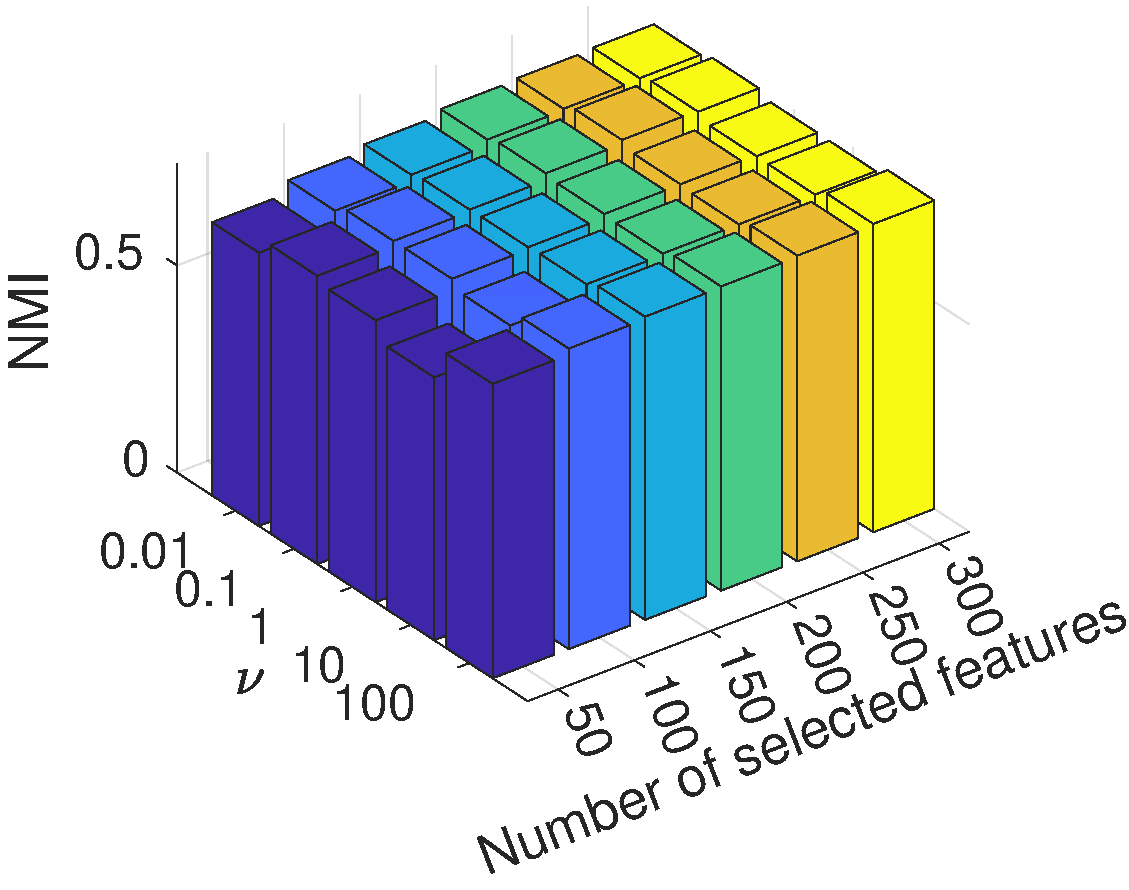
\includegraphics[width=0.33\linewidth]{figures/CPUFS/sensitivity/COIL20_nu.pdf}}
    \subfloat[COIL20 ($\alpha$)\label{fig:l2}]{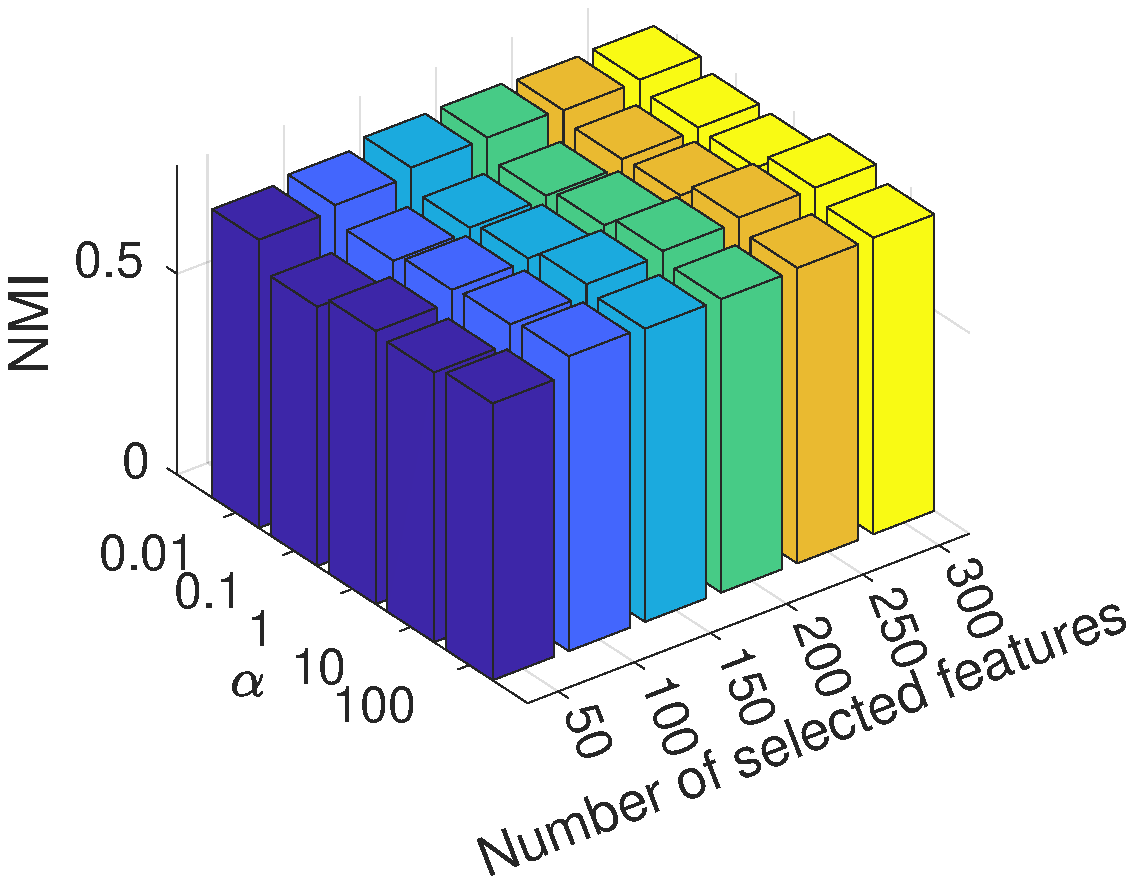
\includegraphics[width=0.33\linewidth]{figures/CPUFS/sensitivity/COIL20_alpha.pdf}}
    \subfloat[COIL20 ($\beta$)\label{fig:l3}]{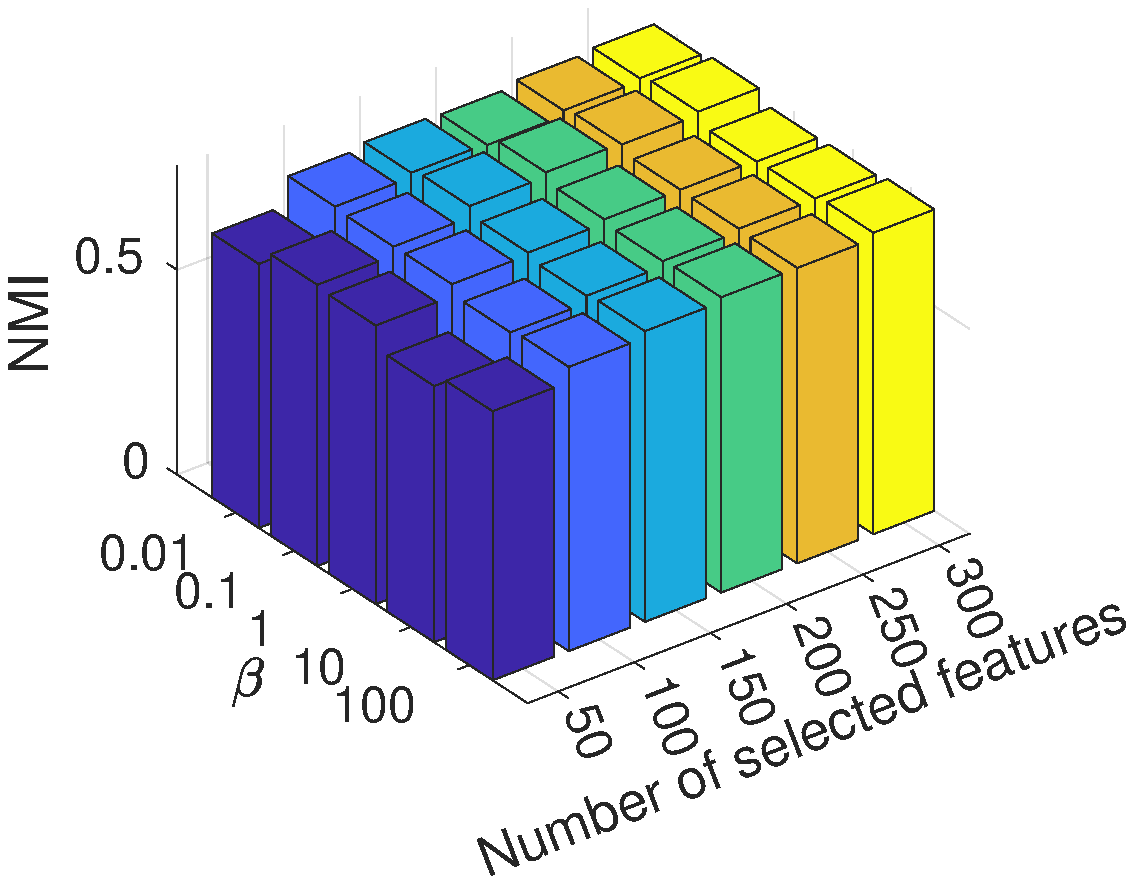
\includegraphics[width=0.33\linewidth]{figures/CPUFS/sensitivity/COIL20_beta.pdf}}\\
    \subfloat[UMIST ($\nu$)\label{fig:w1}] {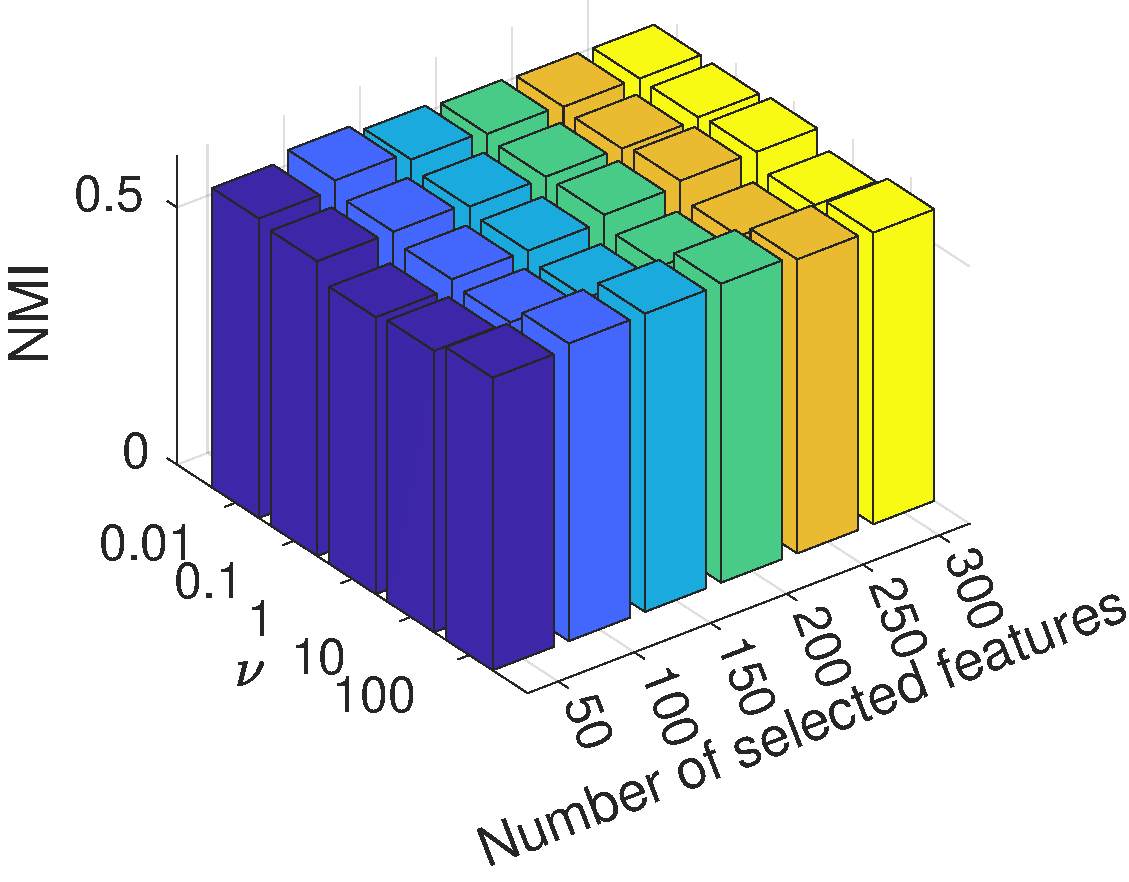
\includegraphics[width=0.33\linewidth]{figures/CPUFS/sensitivity/umist_nu.pdf}}
    \subfloat[UMIST ($\alpha$)\label{fig:w2}]{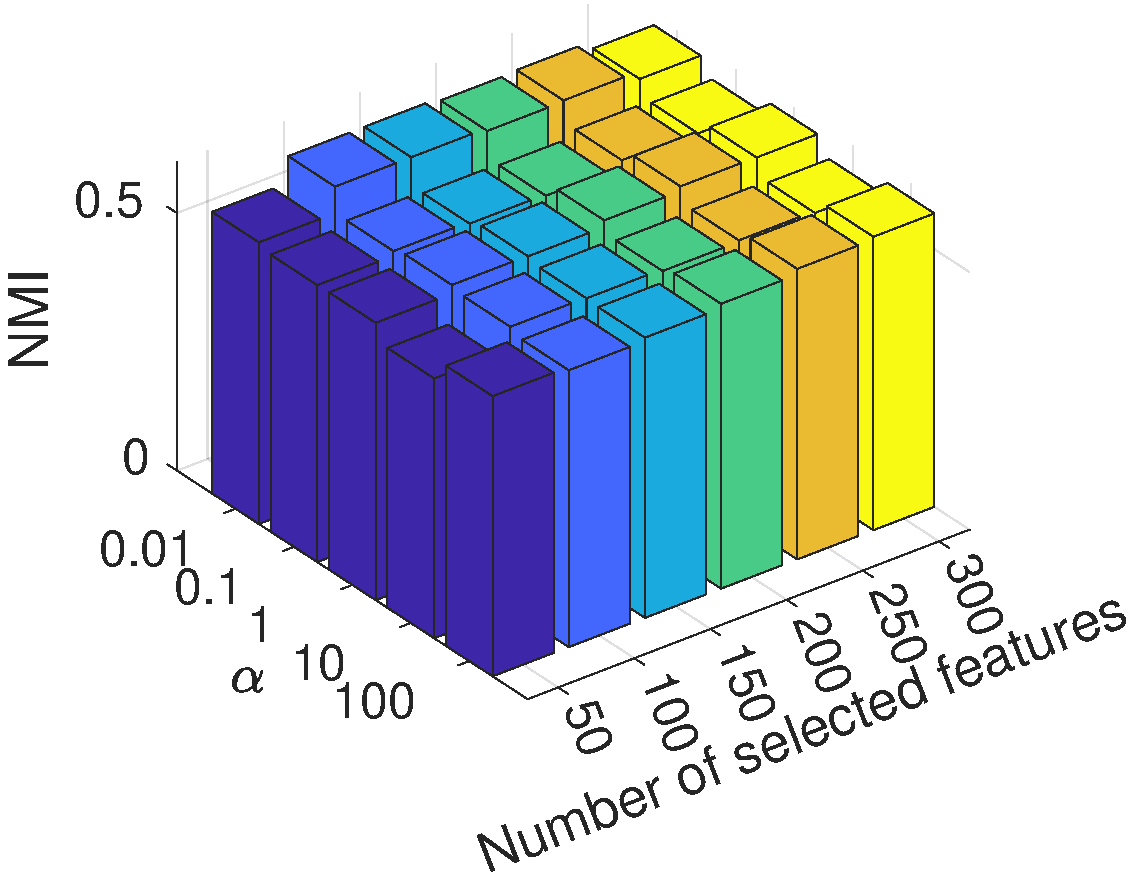
\includegraphics[width=0.33\linewidth]{figures/CPUFS/sensitivity/umist_alpha.pdf}}
    \subfloat[UMIST ($\beta$)\label{fig:w3}]{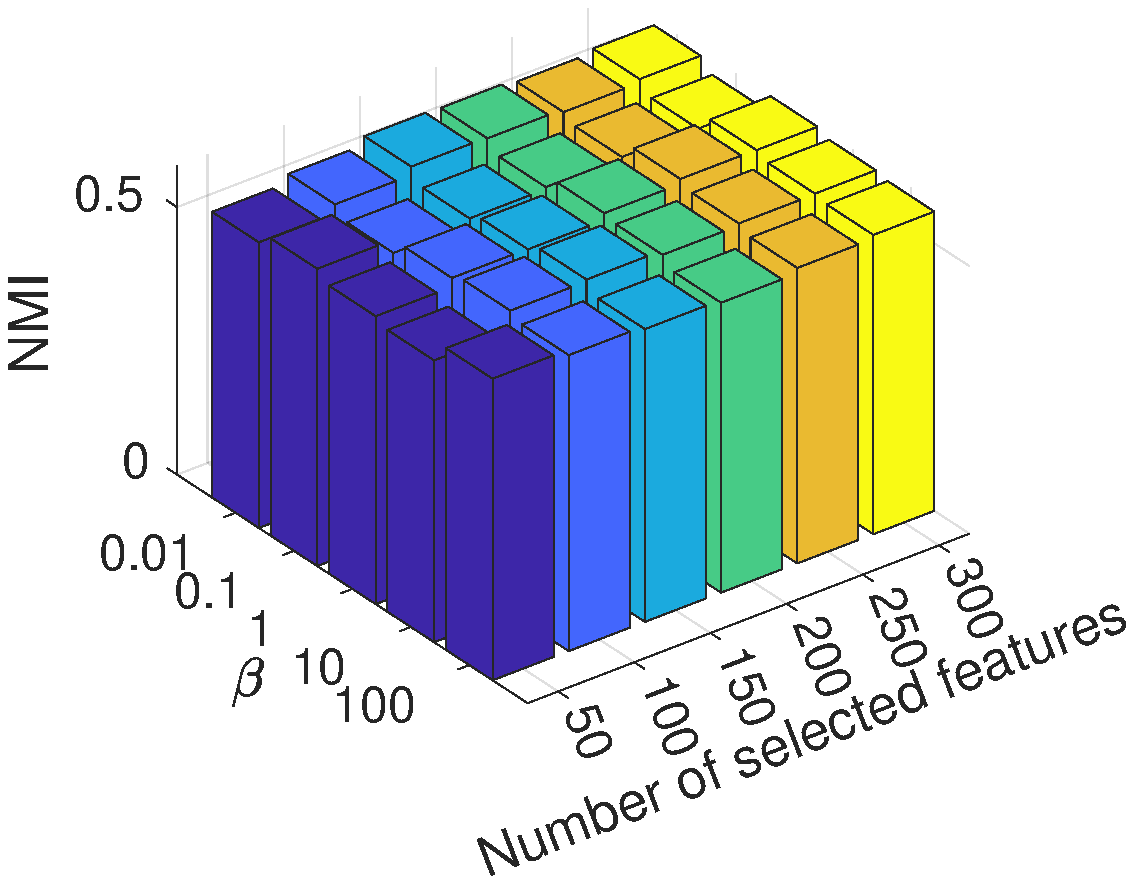
\includegraphics[width=0.33\linewidth]{figures/CPUFS/sensitivity/umist_beta.pdf}}
    \caption{CPUFS方法在FashionMNIST、COIL20与UMIST数据集上的参数敏感度分析}
    \label{fig:sensitivity}
\end{figure}
    
\subsection{参数敏感度分析}
\esubsection{Parameter Sensitivity Analysis}
本节分析CPUFS方法中的参数$\nu$、$\alpha$以及$\beta$对其特征选择性能的影响。具体来说,这些参数交替地在范围$\{10^{-2},10^{-1},1,10,10^{2}\}$内被调整,并且当某个参数被调整时,其余参数均被固定为$1$,然后记录在所有可能的参数组合下CPUFS方法的特征选择性能(由NMI来评价)。实验结果如\reffig{fig:sensitivity}所示。由\reffig{fig:sensitivity},可以得出以下结论:
\begin{enumerate}
\item 在FashionMNIST和COIL20数据集上,当被选择特征的数量较低时(如$50$或$100$),CPUFS方法的性能对这些参数相对敏感,而在其它情况下对这些参数并不敏感。此外,CPUFS方法的性能与被选择特征的数量大致呈正相关关系。
\item 在UMIST数据集上,CPUFS方法的性能对$\alpha$较为敏感,而对其它参数均不敏感。此外,CPUFS方法的性能与被选择特征的数量也不存在显著的相关性。
\end{enumerate}
% 总体而言,CPUFS方法的性能相对于这些参数是较为稳定的。

\subsection{优化效率与收敛性分析}
\esubsection{Optimization Efficiency and Convergence Analyses}
本节首先分析CPUFS方法的优化效率。本文曾在\refsection{sec:companal}分析道,CPUFS方法的优化算法的计算复杂度与数据中的特征数量仅呈线性关系。为了进一步说明理论分析,分别在Pixraw10P、Orlraws10P以及JAFFE数据集上(这三个数据集具有最大的特征数量,因此它们更适合于比较优化效率)运行CPUFS、NDFS、UDFS与RSFS方法(所有方法的所有参数均被固定为$1$),然后记录这四个方法在这三个数据集上的$50$次迭代内的累积时间消耗。实验结果如\reffig{fig:runtime}所示。可以观察到,CPUFS方法与NDFS、UDFS和RSFS方法相比具有明显的优化效率优势,而这个现象符合本文的计算复杂度理论。

\begin{figure}[!t]
    \centering
    \subfloat[Pixraw10P\label{fig:r1}]{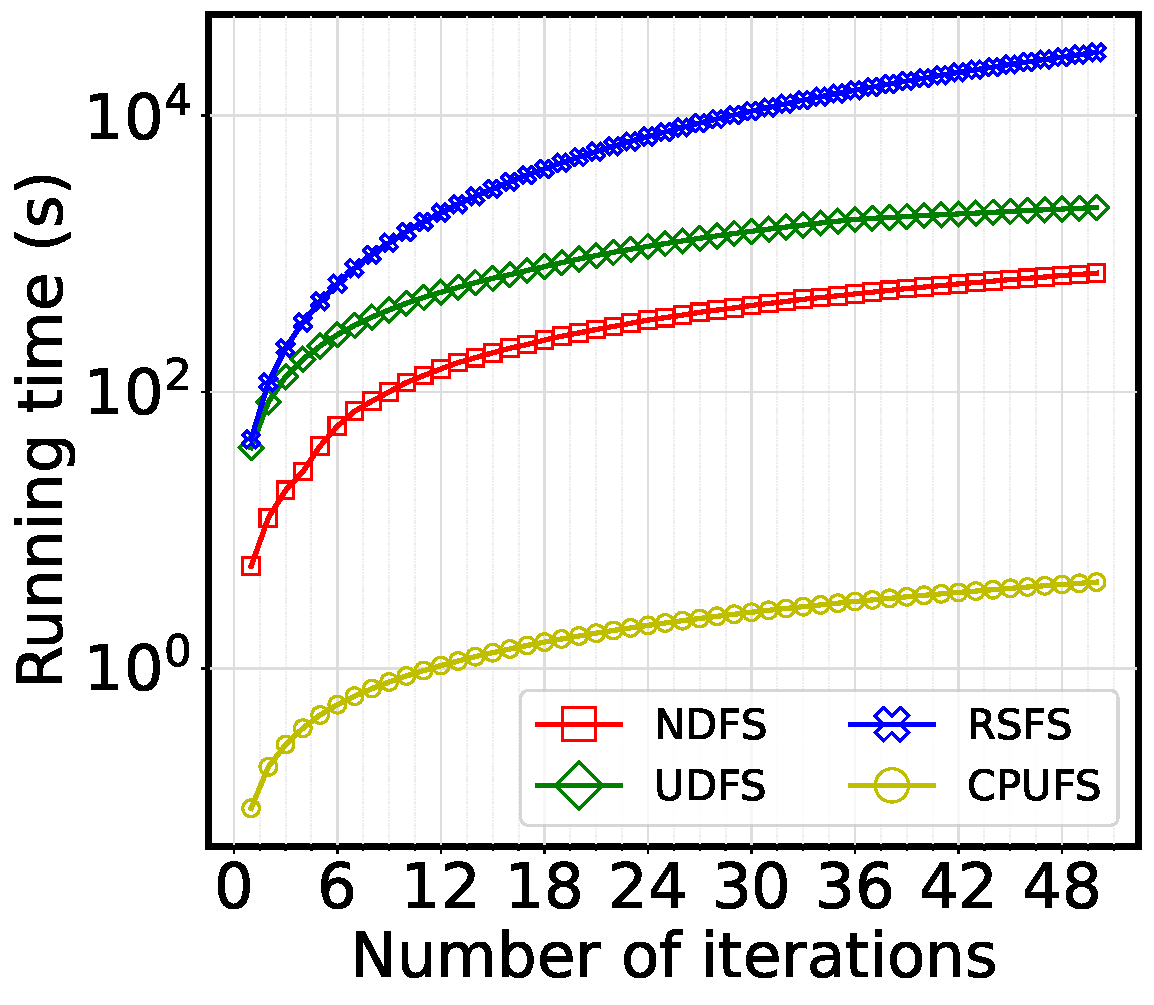
\includegraphics[width=0.33\linewidth]{figures/CPUFS/runtime/CPUFStime_Pixraw10P.pdf}}
    \subfloat[Orlraws10P\label{fig:r2}]{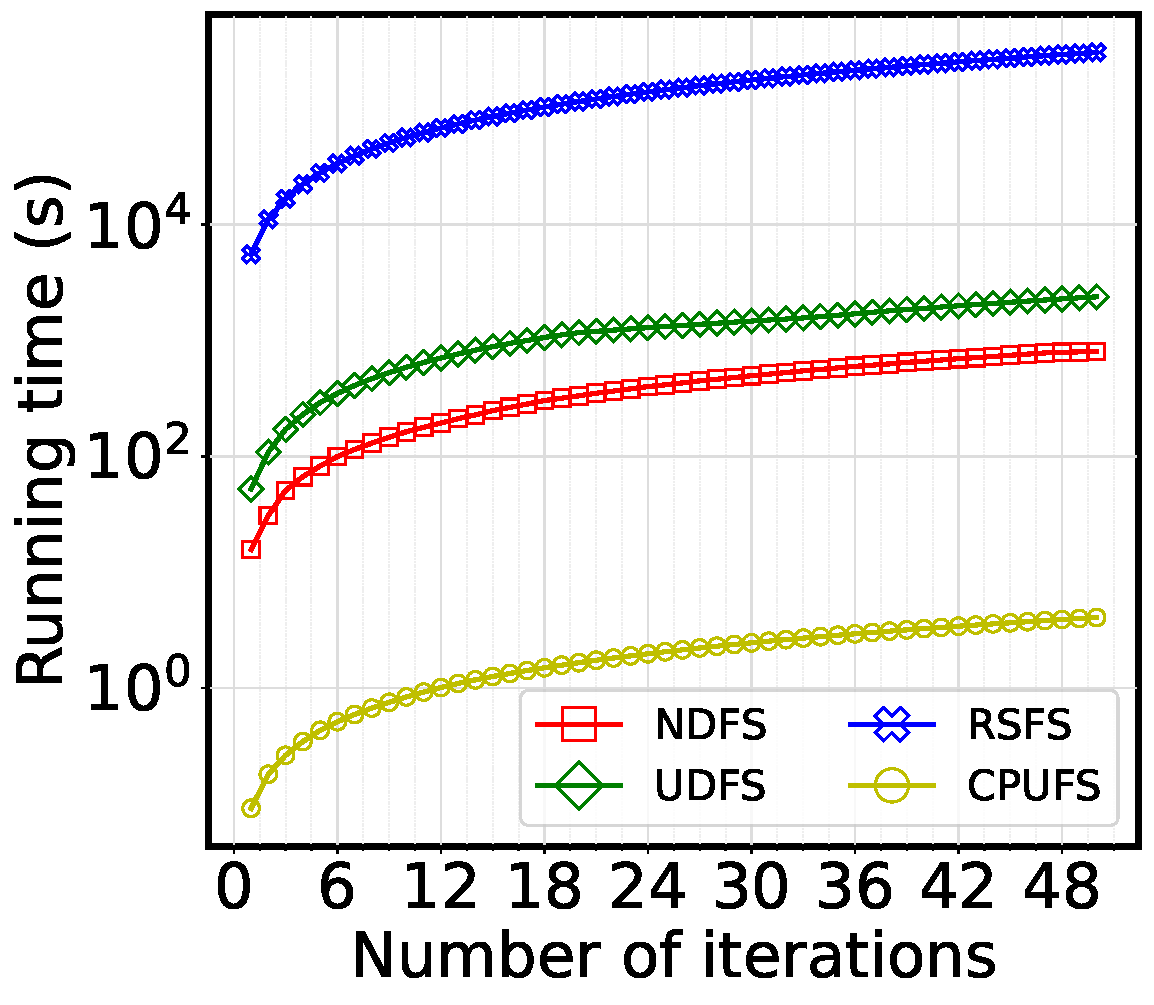
\includegraphics[width=0.33\linewidth]{figures/CPUFS/runtime/CPUFStime_Orlraws10P.pdf}}
    \subfloat[JAFFE\label{fig:r3}]{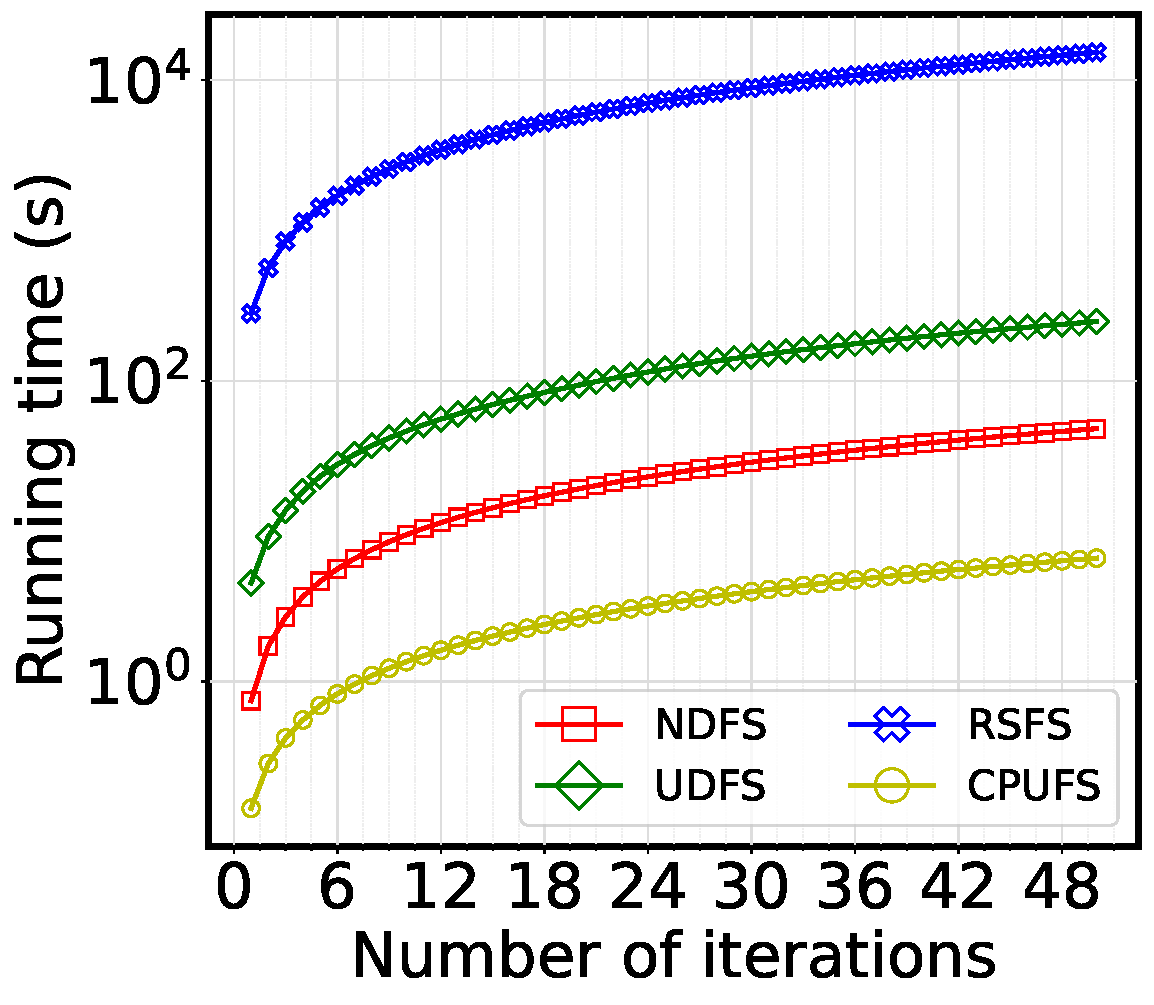
\includegraphics[width=0.33\linewidth]{figures/CPUFS/runtime/CPUFStime_Jaffe.pdf}}
    \caption{CPUFS在Pixraw10P、Orlraws10P与JAFFE数据集上的优化效率分析}
    \label{fig:runtime}
\end{figure}
    
\begin{figure}[!t]
    \centering
    \subfloat[FashionMNIST\label{fig:c1}]{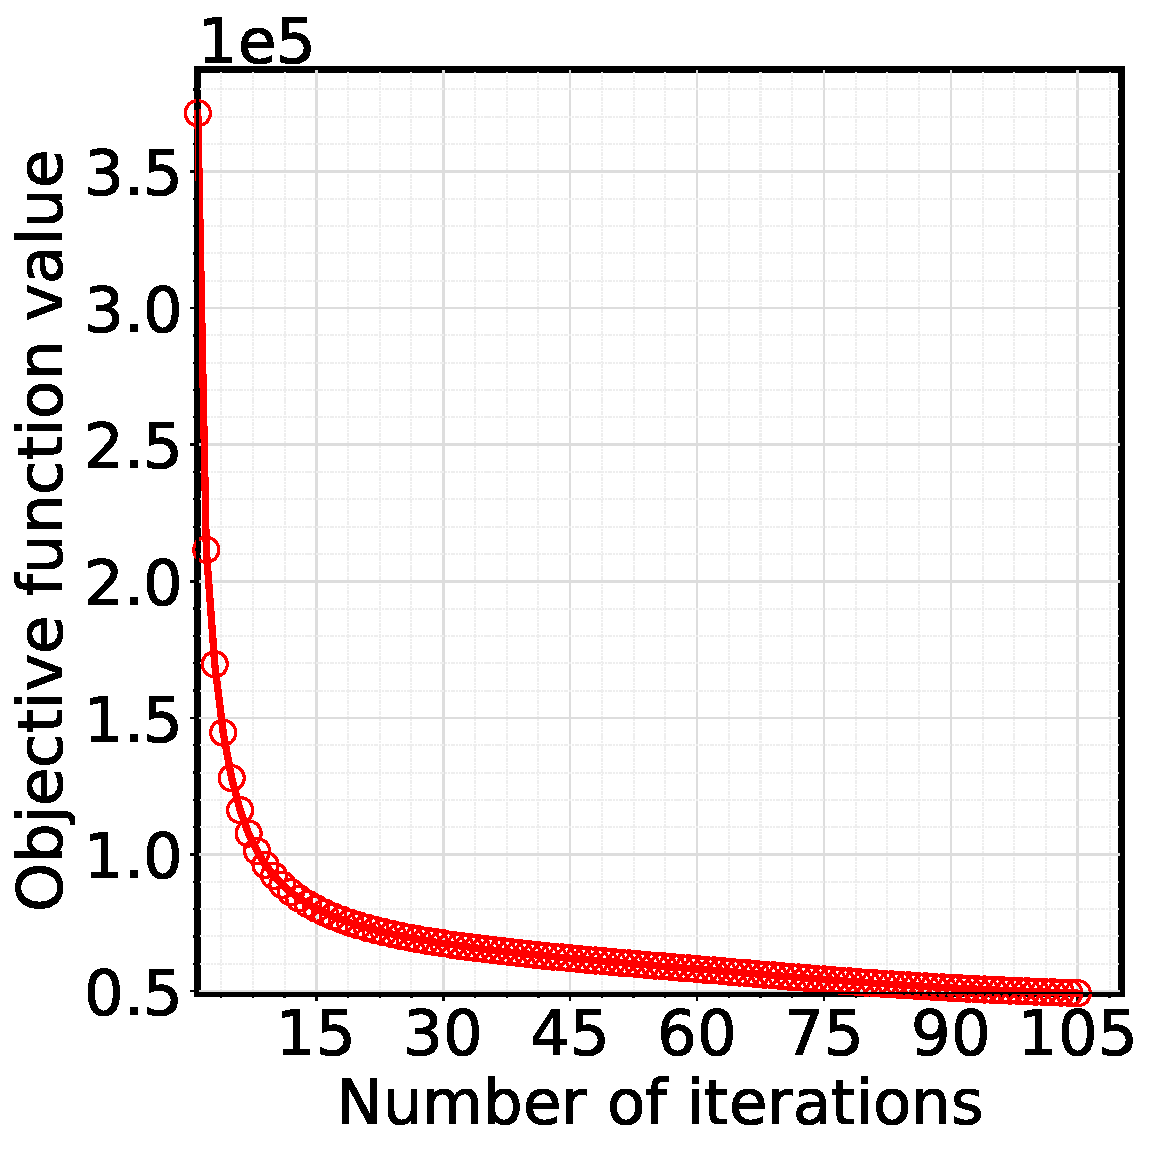
\includegraphics[width=0.33\linewidth]{figures/CPUFS/convergence/loss_fmnist.pdf}}
    \subfloat[COIL20\label{fig:c2}]{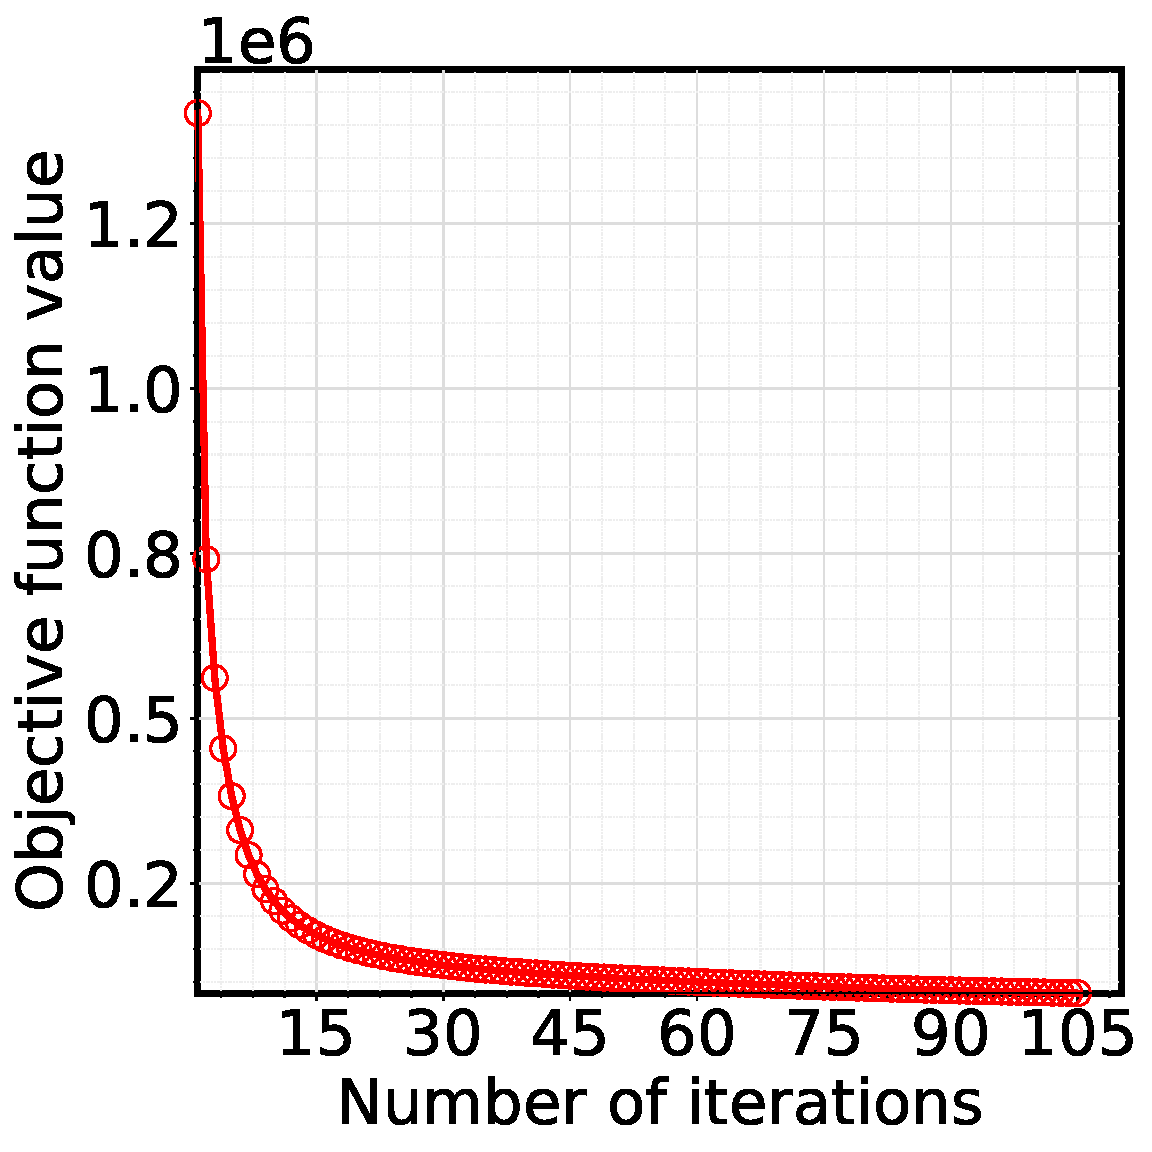
\includegraphics[width=0.33\linewidth]{figures/CPUFS/convergence/loss_COIL20.pdf}}
    \subfloat[UMIST\label{fig:c3}]{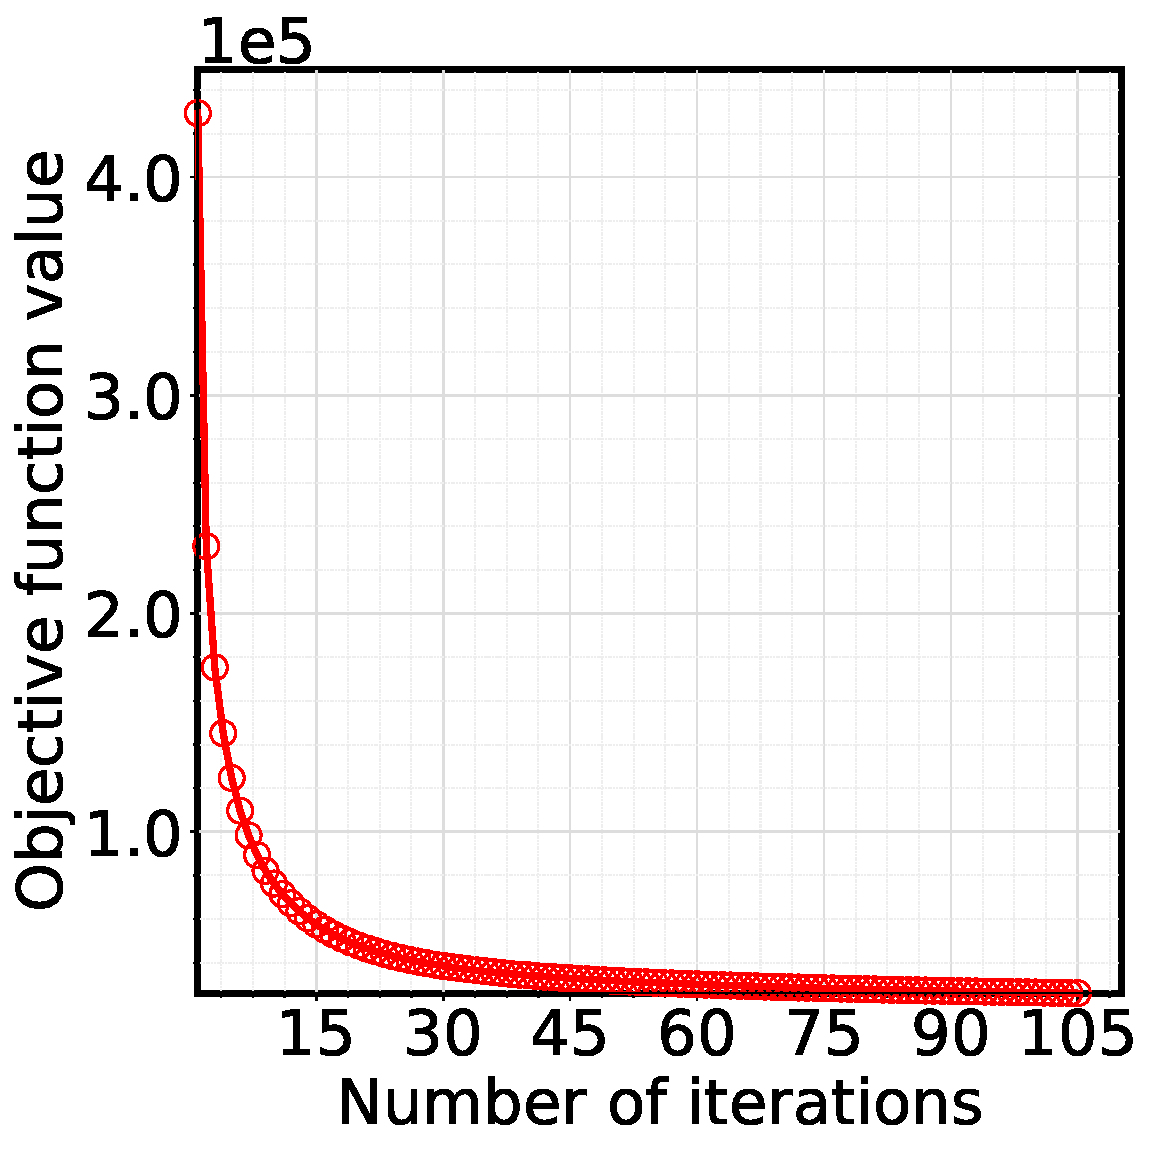
\includegraphics[width=0.33\linewidth]{figures/CPUFS/convergence/loss_umist.pdf}}
    \caption{CPUFS方法在FashionMNIST、COIL20以及UMIST数据集上的收敛性分析}
    \label{fig:converge}
\end{figure}

% \subsection{实验四:收敛性分析}
% \esubsection{Experiment 4: Convergence Analysis}
本节接下来分析CPUFS方法的优化算法的收敛速度。具体来讲,在FashionMNIST、COIL20以及UMIST数据集上运行CPUFS方法(其所有参数均被固定为$1$),并记录其目标函数在每次迭代内的具体数值。记录的目标函数值曲线如\reffig{fig:converge}所示。从\reffig{fig:converge}中可以发现,在这三个数据集上,CPUFS的目标函数值均是单调下降的,而这符合本文的收敛性理论。此外,还可以发现,CPUFS的目标函数值在仅数十次迭代后便降至较低水平,而这反映了CPUFS方法的优化算法的高效性。

\begin{table}[!ht]
    \caption{CPUFS方法与RUFS方法在八个数据集上所选择特征的可视化}\label{tab:visulization}
    \begin{tabular}{>{\centering\arraybackslash}p{0.95in}>{\centering\arraybackslash}p{1.0in}>{\centering\arraybackslash}p{1.0in}>{\centering\arraybackslash}p{1.0in}>{\centering\arraybackslash}p{1.0in}}
        \toprule \diagbox[width=1.2in]{方法}{数据集} & ORL & JAFFE & OCTMNIST & FashionMNIST \\
        \midrule 原始图像 & \parbox[c]{1.0in}{
        
\includegraphics[width=1\linewidth]{figures/CPUFS/visualization/feaOriginal_ORL.pdf}} & \parbox[c]{1.0in}{
        
\includegraphics[width=1\linewidth]{figures/CPUFS/visualization/feaOriginal_JAFFE.pdf}} & \parbox[c]{1.0in}{
        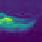
\includegraphics[width=1\linewidth]{figures/CPUFS/visualization/feaOriginal_octmnist.pdf}} & \parbox[c]{1.0in}{
        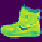
\includegraphics[width=1\linewidth]{figures/CPUFS/visualization/feaOriginal_fmnist.pdf}} \\\addlinespace[0.5em]
        CPUFS & \parbox[c]{1.0in}{
        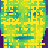
\includegraphics[width=1\linewidth]{figures/CPUFS/visualization/feaCPUFS_ORL.pdf}} & \parbox[c]{1.0in}{
        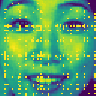
\includegraphics[width=1\linewidth]{figures/CPUFS/visualization/feaCPUFS_JAFFE.pdf}} & \parbox[c]{1.0in}{
        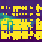
\includegraphics[width=1\linewidth]{figures/CPUFS/visualization/feaCPUFS_octmnist.pdf}} & \parbox[c]{1.0in}{
        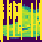
\includegraphics[width=1\linewidth]{figures/CPUFS/visualization/feaCPUFS_fmnist.pdf}} \\\addlinespace[0.5em]
        RUFS & \parbox[c]{1.0in}{
        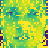
\includegraphics[width=1\linewidth]{figures/CPUFS/visualization/feaRUFS_ORL.pdf}} & \parbox[c]{1.0in}{
        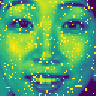
\includegraphics[width=1\linewidth]{figures/CPUFS/visualization/feaRUFS_JAFFE.pdf}} & \parbox[c]{1.0in}{
        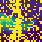
\includegraphics[width=1\linewidth]{figures/CPUFS/visualization/feaRUFS_octmnist.pdf}} & \parbox[c]{1.0in}{
        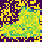
\includegraphics[width=1\linewidth]{figures/CPUFS/visualization/feaRUFS_fmnist.pdf}} \\
        \midrule\midrule \diagbox[width=1.2in]{方法}{数据集} & COIL20 & BreastMNIST & Pixraw10P & Orlraws10P \\
        \midrule 原始图像 & \parbox[c]{1.0in}{
        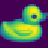
\includegraphics[width=1\linewidth]{figures/CPUFS/visualization/feaOriginal_COIL20.pdf}} & \parbox[c]{1.0in}{
        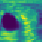
\includegraphics[width=1\linewidth]{figures/CPUFS/visualization/feaOriginal_breastmnist.pdf}} & \parbox[c]{1.0in}{
        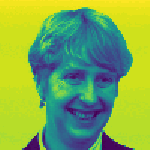
\includegraphics[width=1\linewidth]{figures/CPUFS/visualization/feaOriginal_pixraw10P.pdf}} & \parbox[c]{1.0in}{
        
\includegraphics[width=1\linewidth]{figures/CPUFS/visualization/feaOriginal_orlraws10P.pdf}} \\\addlinespace[0.5em]
        CPUFS & \parbox[c]{1.0in}{
        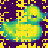
\includegraphics[width=1\linewidth]{figures/CPUFS/visualization/feaCPUFS_COIL20.pdf}} & \parbox[c]{1.0in}{
        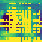
\includegraphics[width=1\linewidth]{figures/CPUFS/visualization/feaCPUFS_breastmnist.pdf}} & \parbox[c]{1.0in}{
        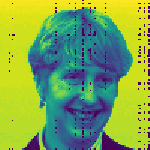
\includegraphics[width=1\linewidth]{figures/CPUFS/visualization/feaCPUFS_pixraw10P.pdf}} & \parbox[c]{1.0in}{
        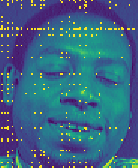
\includegraphics[width=1\linewidth]{figures/CPUFS/visualization/feaCPUFS_orlraws10P.pdf}} \\\addlinespace[0.5em]
        RUFS & \parbox[c]{1.0in}{
        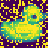
\includegraphics[width=1\linewidth]{figures/CPUFS/visualization/feaRUFS_COIL20.pdf}} & \parbox[c]{1.0in}{
        \includegraphics[width=1\linewidth]{figures/CPUFS/visualization/feaRUFS_breastmnist.pdf}} & \parbox[c]{1.0in}{
        \includegraphics[width=1\linewidth]{figures/CPUFS/visualization/feaRUFS_pixraw10P.pdf}} & \parbox[c]{1.0in}{
        \includegraphics[width=1\linewidth]{figures/CPUFS/visualization/feaRUFS_orlraws10P.pdf}} \\
        \bottomrule
    \end{tabular}
  \end{table}

\subsection{被选择特征的可视化分析}\label{sec:visualization}
\esubsection{Visual Analysis of the Selected Features}
本文曾在\refsection{sec:design-fsmatrix}理论地分析道,在CPUFS方法中,来自数据同一行或同一列的特征具有相互关联的重要性权重。现在展示这种相关性在现实情况下的表征。具体来讲,对于某一数据集,首先检索$300$个就NMI而言表现最好的特征(即该$300$个特征就是达到\reffig{fig:clusnmi}中性能的那些特征)。之后,从该数据集中随机采样一张图像,然后在这张图像上掩盖这$300$个特征并展示。此外,由于CPUFS方法与RUFS方法较为相似,因此本文还使用了同样的方法可视化了RUFS方法所选择的特征。在ORL、JAFFE、OCTMNIST、FashionMNIST、COIL20、BreastMNIST、Pixraw10P以及Orlraws10P这八个数据集上进行了上述实验,实验结果如\reftab{tab:visulization}所示。从\reftab{tab:visulization}可以看出,由CPUFS方法所选择的特征在空间上具有较强的相关性:
\begin{enumerate}
    \item 在FashionMNIST、COIL20以及Pixraw10P数据集上,被选择的特征在垂直方向上具有清晰的结构特性;
    \item 在ORL数据集上,被选择的特征更倾向于聚集在较小的矩形子区域内;
    \item 在JAFFE和Orlraws10P数据集上,被选择的特征显示出了明显的网格状结构;
    \item 在OCTMNIST和BreastMNIST数据集上,被选择的特征更倾向于聚集在一起。
\end{enumerate}
然而,由RUFS方法所选择的特征并没有显示出这样的效果。这种现象充分展示了CPUFS方法作为面向张量的无监督特征选择方法的有效性。本文认为,CPUFS方法的性能提升主要归因于其所选特征的更好结构。

% \begin{figure}[!t]
%     \centering
%     \subfloat[FashionMNIST] {\includegraphics[width=0.32\linewidth]{figures/CPUFS/visualization/feaOriginal_fmnist.pdf}}
%     \hspace{0.01\linewidth}
%     \subfloat[FashionMNIST (CPUFS)]{\includegraphics[width=0.32\linewidth]{figures/CPUFS/visualization/feaCPUFS_fmnist.pdf}}
%     \hspace{0.01\linewidth}
%     \subfloat[FashionMNIST (RUFS)] {\includegraphics[width=0.32\linewidth]{figures/CPUFS/visualization/feaRUFS_fmnist.pdf}}\\
%     \subfloat[COIL20] {\includegraphics[width=0.32\linewidth]{figures/CPUFS/visualization/feaOriginal_COIL20.pdf}}
%     \hspace{0.01\linewidth}
%     \subfloat[COIL20 (CPUFS)]{\includegraphics[width=0.32\linewidth]{figures/CPUFS/visualization/feaCPUFS_COIL20.pdf}}
%     \hspace{0.01\linewidth}
%     \subfloat[COIL20 (RUFS)] {\includegraphics[width=0.32\linewidth]{figures/CPUFS/visualization/feaRUFS_COIL20.pdf}}\\
%     \subfloat[ORL] {\includegraphics[width=0.32\linewidth]{figures/CPUFS/visualization/feaOriginal_ORL.pdf}}
%     \hspace{0.01\linewidth}
%     \subfloat[ORL (CPUFS)]{\includegraphics[width=0.32\linewidth]{figures/CPUFS/visualization/feaCPUFS_ORL.pdf}}
%     \hspace{0.01\linewidth}
%     \subfloat[ORL (RUFS)] {\includegraphics[width=0.32\linewidth]{figures/CPUFS/visualization/feaRUFS_ORL.pdf}}\\
%     \subfloat[Pixraw10P] {\includegraphics[width=0.32\linewidth]{figures/CPUFS/visualization/feaOriginal_pixraw10P.pdf}}
%     \hspace{0.01\linewidth}
%     \subfloat[Pixraw10P (CPUFS)]{\includegraphics[width=0.32\linewidth]{figures/CPUFS/visualization/feaCPUFS_pixraw10P.pdf}}
%     \hspace{0.01\linewidth}
%     \subfloat[Pixraw10P (RUFS)] {\includegraphics[width=0.32\linewidth]{figures/CPUFS/visualization/feaRUFS_pixraw10P.pdf}}\\    
% \end{figure}
% \begin{figure}[!t]
%     \ContinuedFloat
%     \centering
%     \subfloat[Orlraws10P] {\includegraphics[width=0.32\linewidth]{figures/CPUFS/visualization/feaOriginal_orlraws10P.pdf}}
%     \hspace{0.01\linewidth}
%     \subfloat[Orlraws10P (CPUFS)]{\includegraphics[width=0.32\linewidth]{figures/CPUFS/visualization/feaCPUFS_orlraws10P.pdf}}
%     \hspace{0.01\linewidth}
%     \subfloat[Orlraws10P (RUFS)] {\includegraphics[width=0.32\linewidth]{figures/CPUFS/visualization/feaRUFS_orlraws10P.pdf}}\\
%     \subfloat[JAFFE] {\includegraphics[width=0.32\linewidth]{figures/CPUFS/visualization/feaOriginal_jaffe.pdf}}
%     \hspace{0.01\linewidth}
%     \subfloat[JAFFE (CPUFS)]{\includegraphics[width=0.32\linewidth]{figures/CPUFS/visualization/feaCPUFS_JAFFE.pdf}}
%     \hspace{0.01\linewidth}
%     \subfloat[JAFFE (RUFS)] {\includegraphics[width=0.32\linewidth]{figures/CPUFS/visualization/feaRUFS_JAFFE.pdf}}\\
%     \subfloat[BreastMNIST] {\includegraphics[width=0.32\linewidth]{figures/CPUFS/visualization/feaOriginal_breastmnist.pdf}}
%     \hspace{0.01\linewidth}
%     \subfloat[BreastMNIST (CPUFS)]{\includegraphics[width=0.32\linewidth]{figures/CPUFS/visualization/feaCPUFS_breastmnist.pdf}}
%     \hspace{0.01\linewidth}
%     \subfloat[BreastMNIST (RUFS)] {\includegraphics[width=0.32\linewidth]{figures/CPUFS/visualization/feaRUFS_breastmnist.pdf}}\\
%     \subfloat[OCTMNIST] {\includegraphics[width=0.32\linewidth]{figures/CPUFS/visualization/feaOriginal_octmnist.pdf}}
%     \hspace{0.01\linewidth}
%     \subfloat[OCTMNIST (CPUFS)]{\includegraphics[width=0.32\linewidth]{figures/CPUFS/visualization/feaCPUFS_octmnist.pdf}}
%     \hspace{0.01\linewidth}
%     \subfloat[OCTMNIST (RUFS)] {\includegraphics[width=0.32\linewidth]{figures/CPUFS/visualization/feaRUFS_octmnist.pdf}}\\
%     \caption{CPUFS与RUFS在八个数据集上所选择特征的可视化}
%     \label{fig:visulization}
% \end{figure}
% \clearpage
\section{无监督特征提取实验}
\esection{Experiments on Unsupervised Feature Extraction}
% \subsection{实验一:$\ell_{1}$与$\ell_{\infty}$方法和\texorpdfstring{$\ell_{2}$}{L2}方法的性能对比}
% \esubsection{Experiment 1: Comparisons of the $\ell_{1}$ and $\ell_{\infty}$ Methods against the \texorpdfstring{$\ell_{2}$}{L2} Method}
本节将展示无监督特征提取任务的实验结果,并加以分析。
\subsection{性能对比}
\esubsection{Performance Comparison}

\begin{table}[!t]
        \caption{\mbox{$\ell_{1}$、$\ell_{2}$以及$\ell_{\infty}$方法在COIL20数据集上的性能对比}}
        \label{tab:coil}
        \centering
            \begin{tabular}{lcccccc}
    \hline
    \multirow{2}{*}{噪声类型} & \multicolumn{3}{c}{$k$-NN ACC}                                                                         & \multicolumn{3}{c}{SVM ACC}                                                                            \\ \cline{2-7}
                           & $\ell_2$                         & $\ell_1$                         & $\ell_\infty$                    & $\ell_2$                         & $\ell_1$                         & $\ell_\infty$                    \\ \hline
    原始数据               & \textbf{0.9208} & 0.8906                           & {0.8891}       & \textbf{0.9406} & 0.9065                           & 0.9198                           \\
    % \hline\hline
    ms-5-10-20                  & 0.8560                           & 0.8560                           & \textbf{0.8810} & 0.9234                           & 0.9242                           & \textbf{0.9388} \\
    ms-10-10-10 & 0.8435 & 0.8240 & \textbf{0.8990} & 0.9234 & 0.8758 & \textbf{0.9500} \\
    ms-10-20-30 & 0.8224 & 0.7852 & \textbf{0.8406} & 0.9036 & 0.9133 & \textbf{0.9466} \\
    ms-10-30-50 & 0.8221 & 0.8013 & \textbf{0.8721} & 0.9031 & 0.9107 & \textbf{0.9339} \\
    ms-10-50-90 & 0.8128 & 0.7888 & \textbf{0.8664} & 0.9133 & 0.9008 & \textbf{0.9401} \\
    ms-20-20-20 & 0.8159 & 0.8073 & \textbf{0.8698} & 0.9112 & 0.9010 & \textbf{0.9378} \\
    ms-30-30-30 & 0.7901 & 0.8180 & \textbf{0.8768} & 0.9174 & 0.9104 & \textbf{0.9380} \\
    ms-40-40-40 & 0.8076 & 0.8193 & \textbf{0.8964} & 0.9190 & 0.9128 & \textbf{0.9570} \\
    ms-50-50-50 & 0.8250 & 0.8206 & \textbf{0.8680} & 0.9216 & 0.9216 & \textbf{0.9469} \\
    % ms010                  & 0.8068                           & \textbf{0.8836} & {0.8432}       & 0.7211                           & \textbf{0.9307} & 0.8076                           \\
    % ms020                  & 0.5659                           & \textbf{0.8766} & {0.8536}       & 0.4023                           & 0.6763                           & \textbf{0.7685} \\
    % sp002                  & 0.8453                           & 0.8305                           & \textbf{0.8664}       & \textbf{0.9276} & 0.9021                           & 0.9096                           \\
    % sp005                  & 0.8286                           & 0.8237                           & \textbf{0.8721} & 0.9021                           & 0.8938                           & \textbf{0.9026} \\
    % sp007                  & \textbf{0.8372} & 0.8172                           & {0.8076}       & 0.8661                           & 0.8792                           & \textbf{0.8932} \\
    % ms-0-0-0-90                 & 0.8576                           & 0.8375                           & \textbf{0.8826} & 0.9177                           & 0.8977                           & \textbf{0.9187} \\
    ms-5-10-15-20                 & 0.8285                           & 0.7830                           & \textbf{0.8969} & 0.9041                           & 0.8934                           & \textbf{0.9346} \\
    ms-10-10-10-10 & 0.8320 & 0.8391 & \textbf{0.8482} & \textbf{0.9260} & 0.9156 & 0.9115 \\
    ms-10-20-30-40                 & 0.7526                           & 0.7049                           & \textbf{0.8534} & 0.8945                           & 0.8734                           & \textbf{0.9352} \\
    % ms-10-20-30-90 & \textbf{0.7883} & 0.7513 & 0.7781 & 0.8971 & 0.8956 & \textbf{0.9216} \\
    % ms1239                 & \textbf{0.7883} & 0.7513                           & {0.7781}       & 0.8971                           & 0.8956                           & \textbf{0.9216} \\
    ms-10-30-50-70                 & 0.7940                           & 0.7776                           & \textbf{0.8555} & 0.8729                           & 0.9156                           & \textbf{0.9344} \\
    ms-20-20-20-20 & 0.7716 & \textbf{0.8247} & 0.8063 & 0.9078 & 0.9086 & \textbf{0.9245} \\
    ms-30-30-30-30 & 0.7615 & 0.7880 & \textbf{0.8010} & 0.9125 & 0.9159 & \textbf{0.9430} \\
    ms-40-40-40-40 & 0.7596 & 0.7802 & \textbf{0.8526} & 0.9201 & 0.9281 & \textbf{0.9549} \\
    ms-50-50-50-50 & 0.7721 & 0.7974 & \textbf{0.8104} & 0.9190 & 0.9143 & \textbf{0.9385} \\
    \hline\hline
    % sp-1-2-10                  & 0.8461                           & 0.8471                           & \textbf{0.8922} & 0.9180                           & 0.9005                           & \textbf{0.9292} \\
    sp-5-10-20 & 0.8029 & 0.8109 & \textbf{0.8839} & 0.9115 & 0.9026 & \textbf{0.9383} \\
    sp-10-10-10 & 0.7865 & 0.7492 & \textbf{0.8664} & 0.9065 & 0.8841 & \textbf{0.9320} \\
    sp-10-20-30 & 0.7969 & 0.7414 & \textbf{0.8766} & 0.8922 & 0.7859 & \textbf{0.9336} \\
    sp-10-30-50 & 0.7865 & 0.8318 & \textbf{0.8846} & 0.8992 & 0.8901 & \textbf{0.9164} \\
    sp-10-50-90 & 0.8227 & 0.6411 & \textbf{0.8701} & 0.8938 & 0.7299 & \textbf{0.9107} \\
    sp-20-20-20 & 0.7802 & 0.8255 & \textbf{0.8646} & 0.9057 & 0.8896 & \textbf{0.9313} \\
    sp-30-30-30 & 0.7896 & 0.7422 & \textbf{0.8789} & 0.8932 & 0.8401 & \textbf{0.9089} \\
    sp-40-40-40 & 0.8013 & 0.8253 & \textbf{0.8685} & 0.8948 & 0.8690 & \textbf{0.9242} \\
    sp-50-50-50 & 0.8216 & 0.7901 & \textbf{0.8508} & 0.8776 & \textbf{0.8961} & 0.8779 \\
    % sp-0-0-0-20                 & 0.8362                           & 0.8143                           & \textbf{0.9089} & 0.9172                           & 0.9120                           & \textbf{0.9385} \\
    % sp-1-2-5-10                 & 0.8370                           & 0.8292                           & \textbf{0.8966} & 0.9141                           & 0.9062                           & \textbf{0.9398} \\
    sp-5-10-15-20                 & 0.7701                           & 0.7482                           & \textbf{0.8453} & 0.8849                           & 0.8388                           & \textbf{0.9263} \\
    sp-10-10-10-10 & 0.7464 & 0.7878 & \textbf{0.8701} & 0.8781 & 0.8867 & \textbf{0.9286} \\
    sp-10-20-30-40                 & 0.7630                           & 0.6997                           & \textbf{0.8536} & 0.8576                           & 0.7443                           & \textbf{0.9065} \\
    sp-10-30-50-70  & 0.7828 & 0.8180 & \textbf{0.8464} & 0.8888 & 0.8604 & \textbf{0.8992} \\
    sp-20-20-20-20 & 0.7456 & 0.7990 & \textbf{0.8268} & 0.8755 & 0.8724 & \textbf{0.8823} \\
    sp-30-30-30-30 & 0.7609 & 0.6701 & \textbf{0.8406} & 0.8661 & 0.6927 & \textbf{0.8688} \\
    sp-40-40-40-40 & 0.7604 & 0.7865 & \textbf{0.8372} & 0.8534 & 0.8581 & \textbf{0.8747} \\
    sp-50-50-50-50 & 0.7576 & 0.5669 & \textbf{0.8052} & \textbf{0.8612} & 0.6635 & 0.8414 \\
    \hline
    \end{tabular}%
        
\end{table}

    % \guanrmvspace
    \begin{table}[!t]
        \vspace{-1em}
        \caption{\mbox{$\ell_{1}$、$\ell_{2}$以及$\ell_{\infty}$方法在Yale数据集上的性能对比}}
        \label{tab:yale}
        \centering
        \begin{tabular}{lcccccc}
    \hline
    \multirow{2}{*}{噪声类型} & \multicolumn{3}{c}{$k$-NN ACC}                                                                          & \multicolumn{3}{c}{SVM ACC}                                                    \\ \cline{2-7}
                           & $\ell_2$                         & $\ell_1$                         & \multicolumn{1}{l}{$\ell_\infty$} & $\ell_2$ & $\ell_1$                         & $\ell_\infty$                    \\ \hline
    原始数据               & \textbf{0.6370} & 0.6222                           & 0.5556                            & 0.7407   & \textbf{0.7556} & 0.7407                           \\
    % \hline\hline
    % ms-5-10-15 & 0.4593 & 0.4519 & \textbf{0.5630} & \textbf{0.7704} & 0.7556 & \textbf{0.7704} \\
    ms-5-10-20 & 0.3481 & 0.5259 & \textbf{0.6000} & 0.7852 & 0.7556 & \textbf{0.8148} \\
    ms-10-10-10 & 0.4074 & \textbf{0.4667} & 0.4074 & 0.7407 & \textbf{0.7704} & \textbf{0.7704} \\
    ms-10-20-30 & 0.3852 & 0.4815 & \textbf{0.4963} & 0.7556 & 0.7630 & \textbf{0.7852} \\
    ms-10-30-50 & 0.4444 & 0.4889 & \textbf{0.5259} & 0.7704 & 0.7630 & \textbf{0.8222} \\
    ms-10-50-90 & 0.3852 & \textbf{0.5333} & 0.4963 & 0.7333 & 0.7407 & \textbf{0.7704} \\
    ms-20-20-20 & 0.2963 & 0.4296 & \textbf{0.4593} & 0.7778 & 0.7704 & \textbf{0.7926} \\
    ms-30-30-30 & 0.4000 & \textbf{0.4963} & 0.4444 & 0.7778 & \textbf{0.8296} & 0.7778 \\
    ms-40-40-40 & 0.4148 & \textbf{0.5111} & 0.4519 & \textbf{0.8148} & 0.8000 & 0.7111 \\
    ms-50-50-50 & \textbf{0.4370} & \textbf{0.4370} & 0.3852 & 0.7259 & 0.7333 & \textbf{0.7407} \\
    \hline\hline
    % sp-1-3-5                  & 0.4593                           & 0.4889                           & \textbf{0.5852}  & 0.8074   & 0.7333                           & \textbf{0.8222} \\
    sp-5-10-20  & 0.3333 & 0.4519 & \textbf{0.6296} & 0.7111 & 0.7778 &  \textbf{0.8370} \\
    sp-10-10-10 & 0.3259 & \textbf{0.4519} & 0.4148 & 0.7407 & 0.7704 & \textbf{0.7926} \\
    sp-10-20-30                  & 0.4444                           & \textbf{0.4889} & 0.4074                            & 0.7111   & 0.8222                           & \textbf{0.8296} \\
    % sp-10-20-50                  & 0.3185                           & 0.4000                           & \textbf{0.4148}  & 0.6815   & 0.6889                           & \textbf{0.7111} \\
    sp-10-30-50                 & 0.4000                           & 0.5185                           & \textbf{0.5333}  & 0.6519   & 0.7481                           & \textbf{0.8296} \\
    sp-10-50-90  & 0.4074 & \textbf{0.5852} & 0.4593 & 0.6519 & \textbf{0.7704} & 0.7481 \\
    sp-20-20-20 & 0.3407 & \textbf{0.5407} & 0.4963 & 0.6370 & \textbf{0.7556} & 0.7333 \\
    sp-30-30-30 & 0.4444 & 0.5259 & \textbf{0.5704} & 0.5630 & \textbf{0.6593} & \textbf{0.6593} \\
    sp-40-40-40 & 0.4074 & \textbf{0.5926} & 0.5704 & 0.5333 & 0.5333 & \textbf{0.5778} \\
    sp-50-50-50 & 0.3778 & 0.4296 & \textbf{0.5185} & 0.4889 & 0.5037 & \textbf{0.5556} \\
    % sp015                  & 0.2667                           & 0.3926                           & \textbf{0.4963}  & 0.5704   & \textbf{0.7333} & 0.7259                           \\
    % ms000                  & 0.3852                           & 0.4593                           & \textbf{0.5111}  & 0.7185   & \textbf{0.7926} & 0.7852                           \\
    \hline
    \end{tabular}%
        
    \end{table}
    
    \begin{table}[!t]
        \vspace{-0.5em}
        \caption{\mbox{$\ell_{1}$、$\ell_{2}$以及$\ell_{\infty}$方法在UMIST数据集上的性能对比}}
        \label{tab:umist}
        \centering
            \begin{tabular}{lcccccc}
    \hline
    \multirow{2}{*}{噪声类型} & \multicolumn{3}{c}{$k$-NN ACC}                          & \multicolumn{3}{c}{SVM ACC}                                                    \\ \cline{2-7}
                           & $\ell_2$ & $\ell_1$ & \multicolumn{1}{c}{$\ell_\infty$} & $\ell_2$ & $\ell_1$                         & $\ell_\infty$                    \\ \hline
    原始数据               & 0.8281   & 0.8466   & \textbf{0.8546}        & 0.8755   & 0.9133                           & \textbf{0.9181} \\
    % \hline\hline
    % ms00                  & 0.7446   & 0.7357   & \textbf{0.8361}  & 0.8514   & 0.8610                           & \textbf{0.9301} \\
    % rn00                   & 0.7703   & 0.7807   & \textbf{0.8554}  & 0.8562   & 0.8916                           & \textbf{0.9398} \\
    % rn000                  & 0.8249   & 0.8313   & \textbf{0.8474}        & 0.8924   & \textbf{0.9076} & 0.8932                           \\
    % ms00                   & 0.7478   & 0.7406   & \textbf{0.8169}  & 0.8410   & 0.8691                           & \textbf{0.9157} \\
    % sp00                   & 0.7133   & 0.7004   & \textbf{0.8394}  & 0.8225   & 0.7984                           & \textbf{0.9189} \\
    ms-5-10-20 & 0.7912 & 0.8193 & \textbf{0.8482} & 0.8554 & 0.8851 & \textbf{0.8900} \\
    ms-10-10-10 & 0.7727 & 0.8104 & \textbf{0.8217} & 0.8586 & 0.9036 & \textbf{0.9341} \\
    ms-10-20-30                  & 0.7534   & 0.7590   & \textbf{0.7928}  & 0.8378   & 0.8635                           & \textbf{0.9253} \\
    ms-10-30-50  & 0.7823 & 0.7454 & \textbf{0.7888} & 0.8281 & 0.8643 & \textbf{0.8980} \\
    ms-10-50-90                  & 0.7028   & 0.7293   & \textbf{0.8008}  & 0.8217   & 0.8699                           & \textbf{0.8803} \\
    ms-20-20-20  & 0.7365 & 0.7486 & \textbf{0.8080} & 0.8514 & 0.8787 & \textbf{0.9341} \\
    ms-30-30-30  & 0.7157 & 0.7028 & \textbf{0.8000} & 0.8434 & 0.8795 & \textbf{0.9036} \\
    ms-40-40-40  & 0.7261 & 0.7269 & \textbf{0.8080} & 0.8538 & 0.8699 & \textbf{0.9124} \\
    ms-50-50-50  & 0.7277 & 0.7084 & \textbf{0.8048} & 0.8120 & 0.8265 & \textbf{0.8675} \\
    \hline\hline
    % sp00                   & 0.7036   & 0.6924   & \textbf{0.8490}  & 0.8177   & 0.8233                           & \textbf{0.9197} \\
    sp-5-10-20 & 0.7446 & 0.7293 & \textbf{0.8313} & 0.8643 & 0.8795 & \textbf{0.9357} \\
    sp-10-10-10 & 0.6867 & 0.6876 & \textbf{0.7823} & 0.7920 & 0.8072 & \textbf{0.8787} \\
    sp-10-20-30                  & 0.6546   & 0.6506   & \textbf{0.7679}  & 0.7550   & 0.7719                           & \textbf{0.8771} \\
    sp-10-30-50  & 0.6900 & 0.6739 & \textbf{0.8209} & 0.8297 & 0.8233 & \textbf{0.9221} \\
    sp-10-50-90  & 0.7261 & 0.7044 & \textbf{0.8281} & 0.7622 & 0.8000 & \textbf{0.8795} \\
    sp-20-20-20  & 0.6554 & 0.6731 & \textbf{0.7944} & 0.7815 & 0.7960 & \textbf{0.8916} \\
    sp-30-30-30  & 0.6908 & 0.6803 & \textbf{0.7855} & 0.7871 & 0.7888 & \textbf{0.9076} \\
    sp-40-40-40  & 0.7454 & 0.7550 & \textbf{0.8225} & 0.8129 & 0.8498 & \textbf{0.9020} \\
    sp-50-50-50  & 0.7606 & 0.6659 & \textbf{0.8586} & 0.8514 & 0.6514 & \textbf{0.9293} \\
    \hline
    \end{tabular}%
        
    \end{table}
    
本节首先通过在不同噪声场景下的图像分类和人脸识别任务来评估$\ell_{1}$、$\ell_{2}$以及$\ell_{\infty}$方法的性能。具体来讲,首先分别使用$\ell_{1}$、$\ell_{2}$以及$\ell_{\infty}$方法在\refsection{sec:expsetup-ufe}中所提及的所有带噪声数据集中进行特征提取,然后基于被提取的特征使用$k$近邻分类器以及支持向量机分类器进行图像分类与人脸识别,并依据分类准确率来评估不同特征提取方法的性能。实验结果如\reftab{tab:coil}、\reftab{tab:yale}以及\reftab{tab:umist}所示,其中粗体代表最佳的性能数值。从这些表格中,可以得出以下结论:
\begin{enumerate}
    \item \textbf{$\ell_{\infty}$方法非常有效:} 如这些表格所示,在大多数情况下,$\ell_{\infty}$方法相比于$\ell_{2}$以及$\ell_{1}$方法都展现出了显著的性能提升。例如,在COIL20(sp-10-20-30-40)数据集上,就$k$-NN ACC而言,$\ell_{\infty}$方法的性能相比于$\ell_{2}$以及$\ell_{1}$方法分别提升了约$10\%$和$20\%$。除此之外,尽管$\ell_{\infty}$方法在Yale数据集的一些噪声场景下的性能不如$\ell_{1}$方法,但它的整体表现仍然出色,并且在很多情况下要远优于$\ell_{2}$方法。这些现象充分说明了$\ell_{\infty}$方法的有效性。
    \item \textbf{$\ell_{1}$方法也表现尚可:}例如在Yale数据集上,$\ell_{1}$方法在超过1/3的情况下是最优的。这表明了$\ell_{1}$方法也能在一定程度上抑制数据不确定性所带来的负面影响。
    \item \textbf{$\ell_{\infty}$最适用于噪声情形:}可以发现,在三个没有施加噪声的原始数据集上,$\ell_{\infty}$方法表现地并不是特别好。主要原因是由于$\ell_{\infty}$方法致力于优化数据样本中的最大拟合误差,而这似乎并非是在无噪声条件下的明智选择。在没有噪声的场景中,所有样本都变得近乎同样重要。然而,在有噪声的环境下,$\ell_{\infty}$方法的表现非常优异。因此,当数据中存在噪声时,使用$\ell_{\infty}$方法进行特征提取会是较好的选择。
    \item \textbf{不同的方法适用于不同的数据集:}正如所观察到的那样,尽管$\ell_{\infty}$方法在COIL20以及UMIST数据集上表现地相当出色,但它的性能在Yale数据集上并不如所预期的那样优秀(尽管仍然可圈可点)。而尽管$\ell_{1}$方法在COIL20以及UMIST数据集上的表现不如$\ell_{\infty}$方法,但在Yale数据集上,它的表现却比较突出。这表明不同的方法适用于不同类型的数据集。
\end{enumerate}

% \subsection{实验二:与经典的无监督特征提取方法的性能对比}
% \esubsection{Experiment 2: Comparisons with the Classical Methods}

\begin{table}[!t]
    \centering
    \caption{\mbox{$\ell_{1}$、$\ell_{\infty}$以及六个经典的无监督特征提取方法在三个数据集上的性能对比}}
    \label{tab:comp_res}
    \begin{tabular}{@{}lcccccc@{}}
    \hline
    \multirow{2}{*}{方法} & \multicolumn{3}{c}{$k$-NN ACC}                      & \multicolumn{3}{c}{SVM ACC}                         \\ \cline{2-7}
                           & \makecell{COIL20}  & \makecell{Yale}    & \makecell{UMIST}    & \makecell{COIL20}  & \makecell{Yale}  &   \makecell{UMIST}  \\ \hline
    ProbPCA                & 0.8318                     & 0.4667                     & 0.7012                     & 0.8648                     & 0.5481                     & 0.7671                     \\
    FA                     & 0.7102                     & 0.4889                     & 0.5631                     & 0.7247                     & 0.5852                     & 0.6892                     \\
    IsoMap                 & 0.7354                     & 0.4667                     & 0.7325                     & 0.7578                     & 0.6000                     & 0.7759                     \\
    LLE                    & 0.7130                     & 0.4000                     & 0.7301                     & 0.8148                     & 0.4000                     & 0.7205                     \\
    LapE                   & 0.2599                     & 0.0741                     & 0.2313                     & 0.3734                     & 0.1333                     & 0.2048                     \\
    AE            & 0.3615                     & 0.4296                     & 0.5888                     & 0.6117                     & 0.5333                     & 0.6867                     \\
    $\ell_1$方法          & 0.8318 & 0.5185 & 0.6739 & 0.8901 & 0.7481 & 0.8233 \\ 
    $\ell_\infty$方法          & \textbf{0.8846} & \textbf{0.5333} & \textbf{0.8209} & \textbf{0.9164} & \textbf{0.8296} & \textbf{0.9221} \\ 
    \hline
    \end{tabular}%
    
\end{table}
    
本节接下来通过在不同噪声场景下的图像分类和人脸识别任务来评估$\ell_{1}$、$\ell_{\infty}$以及\refsection{sec:expsetup-ufe}中介绍的其它六个经典无监督特征提取方法的性能。具体来讲,首先分别使用$\ell_{1}$、$\ell_{\infty}$以及\refsection{sec:expsetup-ufe}中介绍的其它六个经典无监督特征提取方法在COIL20(sp-10-30-50)、Yale(sp-10-30-50)以及UMIST(sp-10-30-50)数据集中进行特征提取,然后基于被提取的特征使用$k$近邻分类器以及支持向量机分类器进行图像分类与人脸识别,并依据分类准确率来评估不同特征提取方法的性能。实验结果如\reftab{tab:comp_res}所示,其中粗体代表最佳的性能数值。从\reftab{tab:comp_res}中,可以得出以下结论:
\begin{enumerate}
    \item \textbf{$\ell_{\infty}$方法非常有效:}可以观察到,无论是就$k$-NN ACC还是SVM ACC而言,$\ell_{\infty}$方法都一贯地在这三个带噪声的数据集上具有最高精度。这充分说明了$\ell_{\infty}$方法的有效性,而这主要归因于其鲁棒地考虑了最坏情况下的目标函数。
    \item \textbf{$\ell_{1}$方法也表现尚可:}尽管$\ell_{1}$方法的性能不如$\ell_{\infty}$方法,但其在绝大多数情况下仍然为所有方法中性能次优的方法,并相比于其它六个经典无监督特征提取方法展现出了显著的性能提升。这主要归因于$\ell_{1}$方法采用了$\ell_{1}$范数来计算拟合误差,因而在一定程度上增加了特征提取的鲁棒性。
\end{enumerate}

\begin{figure}[!t]
    \centering
    \subfloat[COIL20(sp-10-30-50)] {\includegraphics[width=0.33\linewidth]{figures/Linf/time/Linf_Coil.pdf}}
    \subfloat[Yale(sp-10-30-50)] {\includegraphics[width=0.33\linewidth]{figures/Linf/time/Linf_Yale.pdf}}
    \subfloat[UMIST(sp-10-30-50)] {\includegraphics[width=0.33\linewidth]{figures/Linf/time/Linf_Umist.pdf}}
    \caption{$\ell_{1}$、$\ell_{2}$以及$\ell_{\infty}$方法在COIL20(sp-10-30-50)、Yale(sp-10-30-50)与UMIST(sp-10-30-50)数据集上的优化效率分析}
    \label{fig:runt}
\end{figure}
    
\subsection{优化效率与收敛性分析}
\esubsection{Optimization Efficiency and Convergence Analyses}
本节首先分析$\ell_{1}$与$\ell_{\infty}$方法的优化效率。具体来讲,分别在COIL20(sp-10-30-50)、Yale(sp-10-30-50)与UMIST(sp-10-30-50)数据集上运行$\ell_{1}$、$\ell_{2}$以及$\ell_{\infty}$方法,并记录它们在$50$次迭代内的累积时间消耗。实验结果如\reffig{fig:runt}所示。正如所观察到的那样,
% $\ell_{1}$、$\ell_{2}$以及$\ell_{\infty}$方法在这三个数据集上训练所需要的运行时间趋势大体上相同。除此之外,
在这三个数据集之中的任意一个上,$\ell_{1}$与$\ell_{\infty}$方法都显著地慢于$\ell_{2}$方法,但是$\ell_{1}$与$\ell_{\infty}$方法所花费的时间近乎相同。这个现象符合本文的计算复杂度理论。
% 这个现象从某种层面上说明了$\ell_{\infty}$方法是比较高效的,因为$\ell_{1}$方法的数学优化方法较为简单。
% 此外,根据我们之前的实验结果,$\ell_{\infty}$方法相比于$\ell_{1}$方法,$\ell_{2}$方法以及其它六个经典无监督特征提取方法都展现出了显著的性能提升。
% 因此,$\ell_{\infty}$方法在有效性和效率之间的建立了一个良好的平衡关系。
% 因此,尽管$\ell_{\infty}$方法所需要的优化时间并不低,但这一切都是值得的。
% 此外,根据我们之前的实验结果,$\ell_{\infty}$方法相比于$\ell_{1}$方法展现出了显著的性能优势,因而$\ell_{\infty}$方法在有效性和效率之间的建立了一个良好的平衡关系。

\begin{figure}[!t]
    \centering
    \subfloat[COIL20(sp-10-30-50)] {\includegraphics[width=0.33\linewidth]{figures/Linf/loss/loss_coil.pdf}}
    \subfloat[Yale(sp-10-30-50)] {\includegraphics[width=0.33\linewidth]{figures/Linf/loss/loss_yale.pdf}}
    \subfloat[UMIST(sp-10-30-50)] {\includegraphics[width=0.33\linewidth]{figures/Linf/loss/loss_umist.pdf}}
    \caption{$\ell_{\infty}$方法在COIL20(sp-10-30-50)、Yale(sp-10-30-50)与UMIST(sp-10-30-50)数据集上的收敛性分析}
    \label{fig:conv}
\end{figure}

% \subsection{实验三:收敛性分析}
% \esubsection{Experiment 4: Convergence Analysis}
本节接下来研究$\ell_{\infty}$方法的优化算法的收敛速度。具体来讲,在COIL20(sp-10-30-50)、Yale(sp-10-30-50)以及UMIST(sp-10-30-50)数据集上运行$\ell_{\infty}$方法,并记录其目标函数在每次迭代内的具体数值。记录的目标函数值曲线如\reffig{fig:conv}所示。正如所观察到的那样,在这三个数据集之中的任意一个上,$\ell_{\infty}$方法的目标函数值都是单调减少的,而这符合本文的收敛性理论。此外,虽然据本文所分析,$\ell_{\infty}$方法的优化算法在每次迭代内的计算复杂度都较高,但其在实际情况中
% 的会在一个较低的迭代次数内收敛。如\reffig{fig:conv}所示,在这三个数据集上,$\ell_{\infty}$方法的优化算法
可以在仅数十次迭代后便收敛,而这在某种程度上反映了$\ell_{\infty}$方法的优化算法其实是非常高效的。
% 这个高效性保证整个特征提取过程的效率。

\section{本章小结}
\esection{Summary of the Chapter}
本章首先介绍了实验设置,包括采用的数据集以及评价指标等等。随后,本章展示了无监督特征选择与提取任务的实验结果并加以分析。实验结果不仅表明了本文提出的方法相比于前沿对比方法的优越性,还符合本文的收敛性理论与计算复杂度理论。
% 还测试了我们所提出方法的运行时间特性、收敛特性、参数敏感度,并对CPUFS方法所选择的特征进行了可视化。
% 对比试验的实验结果表明,
% 无论是就数据特征选择与提取的性能,还是就算法的运行时间而言,
% 此外,我们

\afterpage{\null\newpage}\clearpage
%# -*- coding:utf-8 -*-
\chapter{总结与展望}\label{chap:conc}
\echapter{Conclusion and Future Work}

\section{本文总结}
\esection{Conclusion of the Dissertation}

% \subsection{无监督特征选择部分}
% \esubsection{Part I: Unsupervised Feature Selection}
本文面向无监督特征选择任务提出了一种基于张量优化的方法CPUFS。与现有的无监督特征选择方法不同,CPUFS方法考虑并保留了张量的结构信息。为了求解CPUFS方法,本文设计了一种高效的交替迭代优化算法,并建立了它的理论收敛性保证。此外,本文还从理论上证明了所提出的优化算法的计算复杂度与数据中的特征个数仅呈线性关系,而这保证了整个特征选择过程的效率。此外,本文还提出并研究了CPUFS方法的变体CPUFSnn,其对线性分类器的参数矩阵施加了非负约束,并且本文基于CPUFS方法的优化算法及其理论分析也为CPUFSnn方法设计了优化算法并进行了理论分析。本文在十个真实世界的基准数据集中进行了综合的实验,并且实验结果表明,CPUFS和CPUFSnn方法优于前沿的无监督特征选择方法。此外,本文还通过大量实验测试了CPUFS方法的参数灵敏度并经验地分析了CPUFS方法的运行效率和收敛速度。值得一提的是,CPUFS方法可以被很容易地扩展到更高阶形式。

% \subsection{无监督特征提取部分}
% \esubsection{Part II: Unsupervised Feature Extraction}
除上述贡献外,面向无监督特征提取任务,本文还提出了两种分别基于$\ell_{1}$和$\ell_{\infty}$范数的鲁棒张量Tucker分解方法,用以在具有噪声与离群点的数据中进行鲁棒特征提取。受到机器学习理论以及相关工作的启发,$\ell_1$方法旨在优化所有数据样本中的Tucker分解拟合误差之和以缓和数据不确定性所带来的负面影响。受到鲁棒优化理论的启发,$\ell_\infty$方法旨在优化所有数据样本中的最大Tucker分解拟合误差以进一步增强在带噪声环境下的特征提取的鲁棒性。为了求解所提出的$\ell_1$与$\ell_\infty$方法,本文基于二阶锥规划理论为它们设计了有效的交替迭代优化算法,并建立了它们的理论收敛性保证以及进行了理论计算复杂度分析。本文在三个真实世界的基准数据集上设计了大量人工生成的噪声场景,并在不同噪声场景下进行了综合的实验。实验结果表明,与同类型的$\ell_2$方法以及其它经典的无监督特征提取方法相比,$\ell_\infty$方法的性能优异,提升显著,而$\ell_1$方法也能在某些数据集上展现不俗的效果。此外,本文还通过大量实验测试了$\ell_1$与$\ell_\infty$方法的运行效率以及$\ell_\infty$方法的收敛速度。

\section{未来研究方向}
\esection{Future Research Directions}
基于本文所做的研究工作,本节给出如下的未来研究方向:
\begin{enumerate}
    \item \textbf{赋予CPUFS方法处理带缺失值数据的能力:}在一些真实世界的场景中,数据可能是不完整的。例如,这可能由数据收集不当或受到故意的数据污染导致。但是,如果直接将CPUFS方法应用于这些情形可能会导致效果不佳,这是因为其并没有用于处理缺失数据的内置机制,而这将导致其性能劣化。一种可能的解决方案是将缺失值估计机制融合进CPUFS方法。例如,可以采用文献\ucite{2019TDVM}中的策略,即引入额外的优化变量$\mathbfcal{Z}$来代替$\mathbfcal{X}$在目标函数中的位置,并施加额外的等式约束迫使$\mathbfcal{X}$和$\mathbfcal{Z}$在$\mathbfcal{X}$不缺失的索引处相等。具体来讲,上述提案即如下优化模型
\begin{equation*}\vspace{-0.5em}
    \begin{aligned}
    & \underset{\smash[b]{\substack{\mathclap{\boldsymbol{A},\boldsymbol{B},\boldsymbol{C}}\\\mathclap{\boldsymbol{U},\boldsymbol{V},\boldsymbol{Y},\mathbfcal{Z}}}}}{\min}
    & &  \norm{\mathbfcal{Z}-\left\llbracket \boldsymbol{A}, \boldsymbol{B}, \boldsymbol{C} \right\rrbracket}_{F}^{2} + \nu\operatorname{Tr}\left(\boldsymbol{C}^{\top}\boldsymbol{L}\boldsymbol{C}\right) \\ \span&& + \alpha\norm{\left(\mydiag\left(\mathbfcal{Z}\times_{1}\boldsymbol{U}\times_{2}\boldsymbol{V}\right)\right)^{\top} - \boldsymbol{C}}_{F}^{2} + \beta \norm{\boldsymbol{U}^{\top}\odot\boldsymbol{V}^{\top}}_{2,1}\\
    & \text{s.t.}
    & & \boldsymbol{A}\in \mathbb{R}_{+}^{n_1 \times c},~\boldsymbol{B}\in \mathbb{R}_{+}^{n_2 \times c},~\boldsymbol{C}\in \mathbb{R}_{+}^{n \times c},\\
    \span &&\boldsymbol{C}=\boldsymbol{Y}\left(\boldsymbol{Y}^{\top} \boldsymbol{Y}\right)^{-\frac{1}{2}},~\boldsymbol{Y}\in\{0,1\}^{n\times c},~ x_{i j k}=z_{i j k},~\forall~ (i,j,k)\in\mathcal{M},
    \end{aligned}
\end{equation*}
其中$\mathcal{M}\in\mathbb{N}^{3}$为指标集,指示了$\mathbfcal{X}$中的值不缺失处的索引,而其它符号的意义均与\refsection{sec:opt-model-CPUFS}中相同。
    \item \textbf{研发新型的基于张量优化的无监督特征选择方法:}基于本文所设计的面向张量的线性分类器以及特征选择矩阵,可以很容易地将各种基于矩阵优化的无监督特征选择方法拓展到张量形式。例如,基于SOGFS\ucite{sogfs}中自适应图学习的观点,可以使用多个子空间投影矩阵来将原始数据投影至低维张量子空间并保留其内在结构,然后使用基于张量的度量(如张量Frobenius范数诱导的度量)来建立自适应图。基于这种思路的无监督特征选择方法的优化模型如下
\begin{equation*}\vspace{-0.5em}
\hspace{1em}
\begin{aligned}
& \underset{\smash[b]{\substack{\mathclap{\boldsymbol{S},\boldsymbol{C},\{\boldsymbol{U}_{i}\}_{i=1}^{d}}}}}{\min}\qquad
& &  \sum_{i,j=1}^{n}\left(\norm{\left(\mathbfcal{X}^{(i)}-\mathbfcal{X}^{(j)}\right)\times_{1}\boldsymbol{U}_{1}\times_{2}\boldsymbol{U}_{2}\times_{3}\ldots\times_{d}\boldsymbol{U}_{d}}_{F}^{2}s_{i j}+\alpha s_{i j}^{2}\right) \\\span&&+ \lambda\operatorname{Tr}\left(\boldsymbol{C}^{\top}\boldsymbol{L}_{\boldsymbol{S}}\boldsymbol{C}\right) + \gamma \norm{\boldsymbol{U}_{1}^{\top}\odot\boldsymbol{U}_{2}^{\top}\odot\ldots\odot\boldsymbol{U}_{d}^{\top}}_{2,1}\\
& \text{s.t.}
& & \boldsymbol{S}\boldsymbol{1}_{n}=\boldsymbol{1}_{n},~\boldsymbol{S}\in[0,1]^{n\times n},~\boldsymbol{C}^{\top}\boldsymbol{C}=\boldsymbol{I}_{c},~\boldsymbol{U}_{i}\boldsymbol{U}_{i}^{\top}=\boldsymbol{I}_{m},~\forall~i\in[d],
\end{aligned}
\end{equation*}
其中$\boldsymbol{L}_{\boldsymbol{S}}$为自适应相似度图$\boldsymbol{S}$所对应的拉普拉斯矩阵,$m$为低维张量子空间的维度,$\alpha$、$\lambda$以及$\gamma$为控制目标函数中不同项重要性大小的超参数,而其它符号的意义均与\refsection{sec:CPUFS-extend}中一致。除此之外,还有很多很多其它方法可以被拓展到张量形式。由于思路大体类似,故不再赘述具体做法。
% 我们推测我们的工作或将掀起基于张量优化的无监督特征选择的热潮。
    \item \textbf{为\texorpdfstring{$\ell_\infty$}{L无穷}方法添加合适的正则项:}值得注意的是,$\ell_\infty$方法只是简单的骨架方法。细心的读者可能已经注意到了,$\ell_\infty$方法并没有任何参数需要调整。这是由于$\ell_\infty$方法并不涉及任何正则项。那么,很自然的未来研究方向便是如何向$\ell_\infty$方法添加合适的正则项,并开发高效算法进行求解。例如,作为简单的例子,可以向$\ell_\infty$方法中添加图正则\ucite{cai2010graph,2016MR-NTD}(请参考\refsection{sec:graphreg}),从而使得$\ell_\infty$方法可以进一步捕捉到数据的局部几何结构信息,并由此来进一步提升无监督特征提取的效果。具体来讲,这种思想可以被建模成如下的优化模型
\begin{equation*}
\hspace{1em}
    \begin{aligned}
    &\underset{\smash[b]{\mathclap{\{\mathbfcal{G}^{(i)}\}_{i=1}^{n},\{\boldsymbol{A}^{(j)}\}_{j=1}^{d}}}}{\min}\qquad\quad &&\underset{\mathclap{k\in\{1,2,\ldots,n\}}}{\max}\quad \left\|\mathbfcal{X}^{(k)}-\mathbfcal{G}^{(k)} \times_{1} \boldsymbol{A}^{(1)} \ldots \times_{d} \boldsymbol{A}^{(d)}\right\|_{F}\\
    \span && + \lambda\sum_{p,q=1}^{n}s_{pq}\norm{\mathbfcal{G}^{(p)}-\mathbfcal{G}^{(q)}}_{F}^{2} \\
    &\text{s.t.} && \mathbfcal{G}^{(i)}\in\mathbb{R}_{+}^{r_1 \times r_2 \times \ldots \times r_d},~\forall~i\in[n] ,~\boldsymbol{A}^{(j)}\in \mathbb{R}_{+}^{n_j \times r_j},~\forall~j\in[d],
    \end{aligned}
\end{equation*}
其中,$s_{pq}$代表了局部结构相似度图中第$p$个样本$\mathbfcal{X}^{(p)}$与第$q$个样本$\mathbfcal{X}^{(q)}$之间的相似度(可由\refsection{sec:graphreg}中介绍的方法计算),$\lambda$代表图正则的强度,而其它符号的意义均与\refsection{sec:linf}中相同。通过这样的方式,在原始数据的局部结构上相似的样本将会在低维空间中具有相似的特征表示,从而使被提取特征的质量得到进一步的提升。
\end{enumerate}
% \subsection{赋予CPUFS方法处理带缺失值数据的能力}
% \esubsection{Extending CPUFS for Imcomplete Data}

% \subsection{为CPUFS的\texorpdfstring{$\boldsymbol{U}$}{U}和\texorpdfstring{$\boldsymbol{V}$}{V}子问题设计更有效的解法}
% \esubsection{Designing More Effective Algorithms for the $\boldsymbol{U}$ and $\boldsymbol{V}$ Subproblems in CPUFS}

% \subsection{研发新型的基于张量优化的无监督特征选择方法}
% \esubsection{Developing New Tensor Optimization-Based Unsupervised Feature Selection Methods}

% \subsection{为\texorpdfstring{$\ell_\infty$}{L无穷}方法添加各种正则项}
% \esubsection{Incorporating Regularizations into the $\ell_\infty$ Method}

% \section{本章小结}
% \esection{Summary of the Chapter}
% 本章首先总结了本文所做的工作。随后,本章介绍了一些可行的未来研究方向,以供读者进一步进行相关研究。

\afterpage{\null\newpage}\clearpage
% \include{data/related-technologies}

%参考文献
%# -*- coding:utf-8 -*-
\begin{xmuref}
 \bibliographystyle{xmuthesis} %指定参考文献格式文件
 \bibliography{references/paper}%引入bib文件(参考文献所在文件)
%  \afterpage{\null\newpage}\clearpage
\end{xmuref}

%研究成果
%# -*- coding:utf-8 -*-
\begin{publications}
% [1] 作者列表.论文题目.期刊名称,期刊号(编号),起始页码,年份.

[1] Bilian Chen$^{*}$, \textbf{Jiewen Guan}, Zhening Li. Unsupervised Feature Selection via Graph Regularized Nonnegative CP Decomposition[J]. IEEE Transactions on Pattern Analysis and Machine Intelligence, 2022, Early Access. DOI: \href{https://doi.org/10.1109/TPAMI.2022.3160205}{10.1109/TPAMI.2022.3160205}.

[2] \textbf{Jiewen Guan}, Xin Huang, Bilian Chen$^{*}$. Community-Aware Social Recommendation: A Unified SCSVD Framework (Extended Abstract)[C]. In Proceedings of the 38th IEEE International Conference on Data Engineering, 2022, Accepted.

[3] \textbf{Jiewen Guan}, Xin Huang, Bilian Chen$^{*}$. Community-Aware Social Recommendation: A Unified SCSVD Framework[J]. IEEE Transactions on Knowledge and Data Engineering, 2021, Early Access. DOI: \href{https://doi.org/10.1109/TKDE.2021.3117686}{10.1109/TKDE.2021.3117686}.

[4] Xiaochang Lin, \textbf{Jiewen Guan}, Bilian Chen$^{*}$, Yifeng Zeng$^{**}$. Unsupervised Feature Selection via Orthogonal Basis Clustering and Local Structure Preserving[J]. IEEE Transactions on Neural Networks and Learning Systems, 2021, Early Access. DOI: \href{https://doi.org/10.1109/TNNLS.2021.3083763}{10.1109/TNNLS.2021.3083763}.

[5] Zhehao Zhou, Shenbao Yu, \textbf{Jiewen Guan}, Bilian Chen$^{*}$, Langcai Cao. Modeling Transition Matrix for A Collaborative Rating Prediction Recommendation System via Nonnegative Tensor Decomposition[C]. In Proceedings of the 15th IEEE International Conference on Computer Science \& Education, 2020. DOI: \href{https://doi.org/10.1109/ICCSE49874.2020.9201809}{10.1109/ICCSE49874.2020.\linebreak 9201809}.

\afterpage{\null\newpage}\clearpage

\end{publications}


%附录
% %# -*- coding:utf-8 -*-
\begin{apdix}
\appendix
% \counterwithout{section}{chapter}
\setcounter{chapter}{1}
% \section{\reftheorem{thm:UVcvx}的证明}\label{sec:thmproof}
% \esection{Proof of \refetheorem{thm:UVcvx}}
%     \begin{theorem}\label{theorem:thm0}\kaishu
%         $\norm{(\mydiag(\mathbfcal{X}\times_{1}\boldsymbol{U}\times_{2}\boldsymbol{V}))^{\top} - \boldsymbol{F}}_{F}^{2}$分别对$\boldsymbol{U}$或$\boldsymbol{V}$都是凸的。
%     \end{theorem}
    
%     \begin{proof}
%         我们首先证明$\norm{(\mydiag(\mathbfcal{X}\times_{1}\boldsymbol{U}\times_{2}\boldsymbol{V}))^{\top} - \boldsymbol{F}}_{F}^{2}$对矩阵$\boldsymbol{U}$的每一行$\boldsymbol{u}_{i:}$都是凸的。简单的计算表明
%         \begin{equation*}
%             \nabla_{\boldsymbol{u}_{i:}}^{2}\left(\norm{\left(\mydiag\left(\mathbfcal{X}\times_{1}\boldsymbol{U}\times_{2}\boldsymbol{V}\right)\right)^{\top} - \boldsymbol{F}}_{F}^{2}\right) = 2\sum_{k=1}^{n}\boldsymbol{X}^{(k)}\boldsymbol{v}_{i:}^{\top}\boldsymbol{v}_{i:}{\boldsymbol{X}^{(k)}}^{\top}\succeq 0.
%         \end{equation*}
%         因此,我们可以得出以下结论:$\norm{(\mydiag(\mathbfcal{X}\times_{1}\boldsymbol{U}\times_{2}\boldsymbol{V}))^{\top} - \boldsymbol{F}}_{F}^{2}$对矩阵$\boldsymbol{U}$的每一行$\boldsymbol{u}_{i:}$都是凸的。同样地,我们也可以类似地证明$\norm{(\mydiag(\mathbfcal{X}\times_{1}\boldsymbol{U}\times_{2}\boldsymbol{V}))^{\top} - \boldsymbol{F}}_{F}^{2}$对矩阵$\boldsymbol{V}$的每一行$\boldsymbol{v}_{i:}$也都是凸的。我们在此处省略证明,以防赘述。
%     \end{proof}
    
%     \begin{theorem}\kaishu
%         $\norm{(\mydiag(\mathbfcal{X}\times_{1}\boldsymbol{U}\times_{2}\boldsymbol{V}))^{\top} - \boldsymbol{F}}_{F}^{2}$分别对$\boldsymbol{U}$或$\boldsymbol{V}$都是凸的。
%     \end{theorem}
    
%     \begin{proof}
%         这是由于我们有
%         \begin{equation*}
%         \begin{aligned}
%             &\norm{\left(\mydiag\left(\mathbfcal{X}\times_{1}\left(\lambda\boldsymbol{Z}_{1}+\left(1-\lambda\right)\boldsymbol{Z}_{2}\right)\times_{2}\boldsymbol{V}\right)\right)^{\top} - \boldsymbol{F}}_{F}^{2} \\=& \sum_{i=1}^{c}\norm{\left(\mydiag\left(\mathbfcal{X}\times_{1}\left(\lambda(\boldsymbol{z}_{1})_{i:}+\left(1-\lambda\right)(\boldsymbol{z}_{2})_{i:}\right)\times_{2}\boldsymbol{v}_{i:}\right)\right)^{\top} - \boldsymbol{f}_{i}}_{F}^{2} \\\leq& \sum_{i=1}^{c}\left(\lambda\norm{\left(\mydiag\left(\mathbfcal{X}\times_{1}(\boldsymbol{z}_{1})_{i:}\times_{2}\boldsymbol{v}_{i:}\right)\right)^{\top} - \boldsymbol{f}_{i}}_{F}^{2} + \left(1-\lambda\right)\norm{\left(\mydiag\left(\mathbfcal{X}\times_{1}(\boldsymbol{z}_{2})_{i:}\times_{2}\boldsymbol{v}_{i:}\right)\right)^{\top} - \boldsymbol{f}_{i}}_{F}^{2}\right)\\=& \lambda\norm{\left(\mydiag\left(\mathbfcal{X}\times_{1}\boldsymbol{Z}_{1}\times_{2}\boldsymbol{V}\right)\right)^{\top} - \boldsymbol{F}}_{F}^{2} + \left(1-\lambda\right)\norm{\left(\mydiag\left(\mathbfcal{X}\times_{1}\boldsymbol{Z}_{2}\times_{2}\boldsymbol{V}\right)\right)^{\top} - \boldsymbol{F}}_{F}^{2},
%         \end{aligned}
%         \end{equation*}
%         其中不等号部分使用了\reftheorem{theorem:thm0}。依据凸函数的定义\ucite{boyd2004convex},$\boldsymbol{U}$部分的证明就完成了。同样的证明方法也可应用在$\boldsymbol{V}$上。为了避免冗余,我们不再赘述。
%     \end{proof}
    
%     \begin{lemma}\kaishu
%         $\norm{\boldsymbol{X}}_{2,1}$关于$\boldsymbol{X}$是一个凸函数。
%     \end{lemma}
    
%     \begin{proof}
%         我们首先证明$\ell_{2,1}$范数的确是一种范数。简单的计算表明
%         \begin{itemize}
%             \item $\norm{\boldsymbol{0}}_{2,1}=0$,
%             \item 若$\boldsymbol{X}\in\mathbb{R}^{m\times n}$,则$\norm{\alpha\boldsymbol{X}}_{2,1}=\sum_{j=1}^{m}\norm{\alpha\boldsymbol{x}_{j:}}_{2}=\alpha\sum_{j=1}^{m}\norm{\boldsymbol{x}_{j:}}_{2}=\alpha\norm{\boldsymbol{X}}_{2,1}$,
%             \item 若$\boldsymbol{X}\in\mathbb{R}^{m\times n},\boldsymbol{Y}\in\mathbb{R}^{m\times n}$,则$\norm{\boldsymbol{X}+\boldsymbol{Y}}_{2,1}=\sum_{j=1}^{m}\norm{\boldsymbol{x}_{j:}+\boldsymbol{y}_{j:}}_{2}\leq\sum_{j=1}^{m}\norm{\boldsymbol{x}_{j:}}_{2}+\sum_{j=1}^{m}\norm{\boldsymbol{y}_{j:}}_{2}=\norm{\boldsymbol{X}}_{2,1}+\norm{\boldsymbol{Y}}_{2,1}$,其中不等式部分使用了$\ell_{2}$范数的性质。
%         \end{itemize}
%         因此,$\ell_{2,1}$的确是一种范数。由于所有的范数都是凸的\ucite{boyd2004convex},我们的定理即证。
%     \end{proof}
    
%     \begin{theorem}\kaishu
%         $\norm{\boldsymbol{U}^{\top}\odot\boldsymbol{V}^{\top}}_{2,1}$分别对$\boldsymbol{U}$或$\boldsymbol{V}$都是凸的。
%     \end{theorem}
    
%     \begin{proof}
%         由于
%         \begin{equation*}
%             \operatorname{vec}\left(\boldsymbol{U}^{\top} \odot \boldsymbol{V}^{\top}\right)=\left(\boldsymbol{I}_{n_{1}c} \odot\left(\boldsymbol{V}^{\top}\left(\boldsymbol{I}_{c} \otimes \boldsymbol{1}^{\top}_{n_{1}}\right)\right)\right)\operatorname{vec}\left(\boldsymbol{U}^{\top}\right),
%         \end{equation*}
%         因此,$\boldsymbol{U}\mapsto\boldsymbol{U}^{\top}\odot\boldsymbol{V}^{\top}$可以看作是$\boldsymbol{U}$的一个线性函数。同样地,我们也可以推出,$\boldsymbol{U}^{\top}\odot\boldsymbol{V}^{\top}$也是$\boldsymbol{V}$的一个线性函数。由于凸函数与线性函数的复合函数仍然是凸函数\ucite{boyd2004convex},那我们就得到了我们想要的结论。
%     \end{proof}
    
%     \begin{corollary}
%         $\alpha\norm{(\mydiag(\mathbfcal{X}\times_{1}\boldsymbol{U}\times_{2}\boldsymbol{V}))^{\top} - \boldsymbol{F}}_{F}^{2} + \beta \norm{\boldsymbol{U}^{\top}\odot\boldsymbol{V}^{\top}}_{2,1}$对$\boldsymbol{U}$或$\boldsymbol{V}$分别是凸的。
%     \end{corollary}
    
%     \begin{proof}
%         由于凸函数的非负线性组合仍然还是凸函数\ucite{boyd2004convex},那么我们就得到了我们想要的结论。
%     \end{proof}
    
% \section{非负矩阵分解的Lee-Seung算法及其下降性}\label{sec:nmf-dec}
% \esection{The Lee-Seung Algorithm for Nonnegative Matrix Factorization and Its Decreasability}
% 在这一小节,我们介绍用于优化非负矩阵分解的目标函数的Lee-Seung算法,介绍它的下降性。
% \subsection{非负矩阵分解的典范形式}
% \esubsection{The Canonical Form of Nonnegative Matrix Factorization}
% 给定一个矩阵$\boldsymbol{V}\in\mathbb{R}^{n\times m}$,非负矩阵分解即如下数学优化模型
% \begin{equation*}
%     \begin{aligned}
%     & \underset{\smash[b]{\substack{\boldsymbol{W},\boldsymbol{H}}}}{\min}
%     & &  \norm{\boldsymbol{V}-\boldsymbol{W}\boldsymbol{H}}_{F}^{2}\\
%     & \text{s.t.}
%     & & \boldsymbol{W},~\boldsymbol{H}\geq 0,
%     \end{aligned}
% \end{equation*}
% 其中$\boldsymbol{W}\in\mathbb{R}^{n\times r}$,$\boldsymbol{H}\in\mathbb{R}^{r\times m}$。

% \subsection{Lee-Seung算法}
% \esubsection{The Lee-Seung Algorithm}
% 用于优化非负矩阵分解的经典Lee-Seung算法即反复用如下乘法更新公式迭代更新参数矩阵$\boldsymbol{W}$和$\boldsymbol{H}$。
% \begin{equation*}
% \begin{aligned}
%     \boldsymbol{W}\leftarrow\boldsymbol{W}\oast\left(\frac{\boldsymbol{V}\boldsymbol{H}^{\top}}{\boldsymbol{W}\boldsymbol{H}\boldsymbol{H}^{\top}}\right),~\boldsymbol{H}\leftarrow\boldsymbol{H}\oast\left(\frac{\boldsymbol{W}^{\top}\boldsymbol{V}}{\boldsymbol{W}^{\top}\boldsymbol{W}\boldsymbol{H}}\right).
% \end{aligned}
% \end{equation*}

% 我们把Lee-Seung算法总结至\refalg{alg:leeseung}中。

% \begin{algorithm}[t]
% 	\begin{algorithmic}[1]
% 	\REQUIRE 矩阵$\boldsymbol{V}$。
% 	\ENSURE 优化完毕后的参数矩阵$\boldsymbol{W}$和$\boldsymbol{H}$。
% 	\STATE $k\leftarrow 1$,并随机初始化$\boldsymbol{W}$和$\boldsymbol{H}$;
% 	\WHILE{$k<\Phi$并且算法未收敛}
%     \STATE $\boldsymbol{W}\leftarrow\boldsymbol{W}\oast(({\boldsymbol{V}\boldsymbol{H}^{\top}})\oslash({\boldsymbol{W}\boldsymbol{H}\boldsymbol{H}^{\top}}))$;
%     \STATE $\boldsymbol{H}\leftarrow\boldsymbol{H}\oast(({\boldsymbol{W}^{\top}\boldsymbol{V}})\oslash({\boldsymbol{W}^{\top}\boldsymbol{W}\boldsymbol{H}}))$;
% 	\STATE $k\leftarrow k+1$
% 	\ENDWHILE
% 	\RETURN $\boldsymbol{W}_{k}$以及$\boldsymbol{H}_{k}$;
% 	\end{algorithmic}
% 	\captionsetup{labelsep=period,font=bf}
% 	\caption{Lee-Seung算法}
% 	\label{alg:leeseung}
% \end{algorithm}

% 此外,文献\ucite{lee2001algorithms}还给出了如下关于Lee-Seung算法的下降性定理。

% \begin{lemma}[\ucite{lee2001algorithms}]\label{lemma:lee-desc}\kaishu
%     基于\refalg{alg:leeseung},典范型非负矩阵分解的目标函数$\norm{\boldsymbol{V}-\boldsymbol{W}\boldsymbol{H}}_{F}^{2}$在\refalg{alg:leeseung}的每一步都会得到下降。
% \end{lemma}

% \subsection{Lee-Seung算法的下降性}
% \esubsection{The Decreasability of the Lee-Seung Algorithm}
% 在本小节,我们证明Lee-Seung算法的下降性\footnote{对于Lee-Seung算法收敛性更全面的讨论与证明,我们推荐读者阅读文献\ucite{lin2007convergence}。}。我们首先需要下面几个定义来辅助说明主要的引理。

% \begin{definition}[辅助函数\ucite{lee2001algorithms}]\kaishu
%     若一个函数$\Gamma(\boldsymbol{X},\underline{\boldsymbol{X}})$同时对可行域内所有的$\boldsymbol{X}$和$\underline{\boldsymbol{X}}$满足$\Gamma(\boldsymbol{X},\underline{\boldsymbol{X}})\geq\Psi(\boldsymbol{X})$且$\Gamma(\boldsymbol{X},\boldsymbol{X})=\Psi(\boldsymbol{X})$,那我们说$\Gamma(\boldsymbol{X},\underline{\boldsymbol{X}})$是$\Psi(\boldsymbol{X})$的一个辅助函数。
% \end{definition}
    
% \begin{lemma}[辅助函数的下降性\ucite{lee2001algorithms}]\label{lemma:aux_ppt}\kaishu
% 若$\Gamma(\boldsymbol{X},\underline{\boldsymbol{X}})$为$\Psi(\boldsymbol{X})$的一个辅助函数,则基于更新公式$\boldsymbol{X}_{t+1}=\arg\min_{\boldsymbol{X}}\Gamma(\boldsymbol{X},\boldsymbol{X}_{t})$,$\Psi(\boldsymbol{X})$在每一步都是下降的。
% \end{lemma}
% \begin{proof}
% 这是由于$\Psi(\boldsymbol{X}_{t+1})\leq\Gamma(\boldsymbol{X}_{t+1},\boldsymbol{X}_{t})\leq\Gamma(\boldsymbol{X}_{t},\boldsymbol{X}_{t})=\Psi(\boldsymbol{X}_{t})$.
% \end{proof}

% \begin{lemma}[NMF目标函数的一个辅助函数\ucite{lee2001algorithms}]\kaishu
%     记$\Psi(\boldsymbol{h}_{:i})=(1/2)\norm{\boldsymbol{v}_{:i}-\boldsymbol{W}\boldsymbol{h}_{:i}}_{2}^{2}$。则函数
%     \begin{equation*}
%     \begin{aligned}
%         \Gamma(\boldsymbol{h}_{:i},\underline{\boldsymbol{h}}_{:i})=&\Psi(\underline{\boldsymbol{h}}_{:i})+\left(\boldsymbol{h}_{:i}-\underline{\boldsymbol{h}}_{:i}\right)^{\top}\nabla\Psi(\underline{\boldsymbol{h}}_{:i})\\&+\frac{1}{2}\left(\boldsymbol{h}_{:i}-\underline{\boldsymbol{h}}_{:i}\right)^{\top}
%         \begin{pmatrix}
%             \frac{\left(\boldsymbol{w}_{:1}^{\top}\boldsymbol{W}\underline{\boldsymbol{h}}_{:i}\right)}{\underline{\boldsymbol{h}}_{1i}} & 0 & \ldots & 0\\
%             0 & \frac{\left(\boldsymbol{w}_{:2}^{\top}\boldsymbol{W}\underline{\boldsymbol{h}}_{:i}\right)}{\underline{\boldsymbol{h}}_{2i}} & \ldots & 0\\
%             \vdots & \vdots & \ddots & \vdots\\
%             0 & 0 & \ldots & \frac{\left(\boldsymbol{w}_{:r}^{\top}\boldsymbol{W}\underline{\boldsymbol{h}}_{:i}\right)}{\underline{\boldsymbol{h}}_{ri}}
%         \end{pmatrix}
%         \left(\boldsymbol{h}_{:i}-\underline{\boldsymbol{h}}_{:i}\right)
%     \end{aligned}
%     \end{equation*}
%     为$\Psi(\boldsymbol{h}_{:i})$的一个辅助函数。
% \end{lemma}

% 有了这些定义,我们可以开始叙述Lee-Seung算法的下降性了。下面的引理告诉我们,Lee-Seung算法在每一步$\boldsymbol{H}$更新迭代都能使得非负矩阵分解的目标函数得到下降。
% \begin{lemma}\kaishu
%     基于Lee-Seung算法,每次更新矩阵$\boldsymbol{H}$时,非负矩阵分解的目标函数均会下降。
% \end{lemma}

% \begin{proof}
%     这是由于如果我们将$\arg\min_{\boldsymbol{h}_{:i}}\Gamma(\boldsymbol{h}_{:i},\underline{\boldsymbol{h}}_{:i})$,$\forall~ i=1,2,\ldots,m$的结果拼到一起,那么结果刚好是Lee-Seung算法的$\boldsymbol{H}$更新公式。由\reflemma{lemma:aux_ppt},本引理即证。
% \end{proof}

% 同样地,我们也可以证明Lee-Seung算法在每一步$\boldsymbol{W}$更新迭代都能使得非负矩阵分解的目标函数得到下降。综上,我们得出以下推论。

% \begin{corollary}
%     基于Lee-Seung算法,目标函数在每一步都会得到下降。
% \end{corollary}

\section{无监督特征提取实验中的噪声汇总}\label{sec:noise-comp}
\esection{Compilation of Noisy Data in Experiments of Unsupervised Feature Extraction}
下面这一系列图样,展示了我们在\refsection{sec:dataset}中为无监督特征提取任务设计的一系列噪声的具体表现形式,其中子图的顺序与噪声施加的顺序保持一致。

\begin{sidewaysfigure}[!ht]
\centering
\subfloat[ms-5-10-20] {\frame{\includegraphics[width=0.32\linewidth]{figures/Linf/Linf_corr_imgs/COIL/ms_005-010-020.pdf}}}\hspace{0.001\linewidth}
\subfloat[ms-10-10-10] {\frame{\includegraphics[width=0.32\linewidth]{figures/Linf/Linf_corr_imgs/COIL/ms_010-010-010.pdf}}}\hspace{0.001\linewidth}
\subfloat[ms-10-20-30] {\frame{\includegraphics[width=0.32\linewidth]{figures/Linf/Linf_corr_imgs/COIL/ms_010-020-030.pdf}}}\hspace{0.001\linewidth}
\subfloat[ms-10-30-50] {\frame{\includegraphics[width=0.32\linewidth]{figures/Linf/Linf_corr_imgs/COIL/ms_010-030-050.pdf}}}\hspace{0.001\linewidth}
\subfloat[ms-10-50-90] {\frame{\includegraphics[width=0.32\linewidth]{figures/Linf/Linf_corr_imgs/COIL/ms_010-050-090.pdf}}}\hspace{0.001\linewidth}
\subfloat[ms-20-20-20] {\frame{\includegraphics[width=0.32\linewidth]{figures/Linf/Linf_corr_imgs/COIL/ms_020-020-020.pdf}}}\hspace{0.001\linewidth}
\subfloat[ms-30-30-30] {\frame{\includegraphics[width=0.32\linewidth]{figures/Linf/Linf_corr_imgs/COIL/ms_030-030-030.pdf}}}\hspace{0.001\linewidth}
\subfloat[ms-40-40-40] {\frame{\includegraphics[width=0.32\linewidth]{figures/Linf/Linf_corr_imgs/COIL/ms_040-040-040.pdf}}}\hspace{0.001\linewidth}
\subfloat[ms-50-50-50] {\frame{\includegraphics[width=0.32\linewidth]{figures/Linf/Linf_corr_imgs/COIL/ms_050-050-050.pdf}}}\hspace{0.001\linewidth}
\subfloat[ms-5-10-15-20] {\frame{\includegraphics[width=0.32\linewidth]{figures/Linf/Linf_corr_imgs/COIL/ms_005-010-015-020.pdf}}}\hspace{0.001\linewidth}
\subfloat[ms-10-10-10-10] {\frame{\includegraphics[width=0.32\linewidth]{figures/Linf/Linf_corr_imgs/COIL/ms_010-010-010-010.pdf}}}\hspace{0.001\linewidth}
\subfloat[ms-10-20-30-40] {\frame{\includegraphics[width=0.32\linewidth]{figures/Linf/Linf_corr_imgs/COIL/ms_010-020-030-040.pdf}}}\hspace{0.001\linewidth}
\end{sidewaysfigure}

\begin{sidewaysfigure}[!ht]
\ContinuedFloat
\centering
\subfloat[ms-10-30-50-70] {\frame{\includegraphics[width=0.32\linewidth]{figures/Linf/Linf_corr_imgs/COIL/ms_010-030-050-070.pdf}}}\hspace{0.001\linewidth}
\subfloat[ms-20-20-20-20] {\frame{\includegraphics[width=0.32\linewidth]{figures/Linf/Linf_corr_imgs/COIL/ms_020-020-020-020.pdf}}}\hspace{0.001\linewidth}
\subfloat[ms-30-30-30-30] {\frame{\includegraphics[width=0.32\linewidth]{figures/Linf/Linf_corr_imgs/COIL/ms_030-030-030-030.pdf}}}\hspace{0.001\linewidth}
\subfloat[ms-40-40-40-40] {\frame{\includegraphics[width=0.32\linewidth]{figures/Linf/Linf_corr_imgs/COIL/ms_040-040-040-040.pdf}}}\hspace{0.001\linewidth}
\subfloat[ms-50-50-50-50] {\frame{\includegraphics[width=0.32\linewidth]{figures/Linf/Linf_corr_imgs/COIL/ms_050-050-050-050.pdf}}}\hspace{0.001\linewidth}
\subfloat[sp-5-10-20] {\frame{\includegraphics[width=0.32\linewidth]{figures/Linf/Linf_corr_imgs/COIL/sp_005-010-020.pdf}}}\hspace{0.001\linewidth}
\subfloat[sp-10-10-10] {\frame{\includegraphics[width=0.32\linewidth]{figures/Linf/Linf_corr_imgs/COIL/sp_010-010-010.pdf}}}\hspace{0.001\linewidth}
\subfloat[sp-10-20-30] {\frame{\includegraphics[width=0.32\linewidth]{figures/Linf/Linf_corr_imgs/COIL/sp_010-020-030.pdf}}}\hspace{0.001\linewidth}
\subfloat[sp-10-30-50] {\frame{\includegraphics[width=0.32\linewidth]{figures/Linf/Linf_corr_imgs/COIL/sp_010-030-050.pdf}}}\hspace{0.001\linewidth}
\subfloat[sp-10-50-90] {\frame{\includegraphics[width=0.32\linewidth]{figures/Linf/Linf_corr_imgs/COIL/sp_010-050-090.pdf}}}\hspace{0.001\linewidth}
\subfloat[sp-20-20-20] {\frame{\includegraphics[width=0.32\linewidth]{figures/Linf/Linf_corr_imgs/COIL/sp_020-020-020.pdf}}}\hspace{0.001\linewidth}
\subfloat[sp-30-30-30] {\frame{\includegraphics[width=0.32\linewidth]{figures/Linf/Linf_corr_imgs/COIL/sp_030-030-030.pdf}}}\hspace{0.001\linewidth}
\end{sidewaysfigure}

\begin{sidewaysfigure}[!ht]
\ContinuedFloat
\centering
\subfloat[sp-40-40-40] {\frame{\includegraphics[width=0.32\linewidth]{figures/Linf/Linf_corr_imgs/COIL/sp_040-040-040.pdf}}}\hspace{0.001\linewidth}
\subfloat[sp-50-50-50] {\frame{\includegraphics[width=0.32\linewidth]{figures/Linf/Linf_corr_imgs/COIL/sp_050-050-050.pdf}}}\hspace{0.001\linewidth}
\subfloat[sp-5-10-15-20] {\frame{\includegraphics[width=0.32\linewidth]{figures/Linf/Linf_corr_imgs/COIL/sp_005-010-015-020.pdf}}}\hspace{0.001\linewidth}
\subfloat[sp-10-10-10-10] {\frame{\includegraphics[width=0.32\linewidth]{figures/Linf/Linf_corr_imgs/COIL/sp_010-010-010-010.pdf}}}\hspace{0.001\linewidth}
\subfloat[sp-10-20-30-40] {\frame{\includegraphics[width=0.32\linewidth]{figures/Linf/Linf_corr_imgs/COIL/sp_010-020-030-040.pdf}}}\hspace{0.001\linewidth}
\subfloat[sp-10-30-50-70] {\frame{\includegraphics[width=0.32\linewidth]{figures/Linf/Linf_corr_imgs/COIL/sp_010-030-050-070.pdf}}}\hspace{0.001\linewidth}
\subfloat[sp-20-20-20-20] {\frame{\includegraphics[width=0.32\linewidth]{figures/Linf/Linf_corr_imgs/COIL/sp_020-020-020-020.pdf}}}\hspace{0.001\linewidth}
\subfloat[sp-30-30-30-30] {\frame{\includegraphics[width=0.32\linewidth]{figures/Linf/Linf_corr_imgs/COIL/sp_030-030-030-030.pdf}}}\hspace{0.001\linewidth}
\subfloat[sp-40-40-40-40] {\frame{\includegraphics[width=0.32\linewidth]{figures/Linf/Linf_corr_imgs/COIL/sp_040-040-040-040.pdf}}}\hspace{0.001\linewidth}
\subfloat[sp-50-50-50-50] {\frame{\includegraphics[width=0.32\linewidth]{figures/Linf/Linf_corr_imgs/COIL/sp_050-050-050-050.pdf}}}\hspace{0.001\linewidth}
\caption{COIL20数据集上的带噪声图像示意}
\label{fig:corr-coil}
\end{sidewaysfigure}

\begin{sidewaysfigure}[!ht]
\centering
\subfloat[ms-5-10-20] {\frame{\includegraphics[width=0.32\linewidth]{figures/Linf/Linf_corr_imgs/UMIST/ms_005-010-020.pdf}}}\hspace{0.001\linewidth}
\subfloat[ms-10-10-10] {\frame{\includegraphics[width=0.32\linewidth]{figures/Linf/Linf_corr_imgs/UMIST/ms_010-010-010.pdf}}}\hspace{0.001\linewidth}
\subfloat[ms-10-20-30] {\frame{\includegraphics[width=0.32\linewidth]{figures/Linf/Linf_corr_imgs/UMIST/ms_010-020-030.pdf}}}\hspace{0.001\linewidth}
\subfloat[ms-10-30-50] {\frame{\includegraphics[width=0.32\linewidth]{figures/Linf/Linf_corr_imgs/UMIST/ms_010-030-050.pdf}}}\hspace{0.001\linewidth}
\subfloat[ms-10-50-90] {\frame{\includegraphics[width=0.32\linewidth]{figures/Linf/Linf_corr_imgs/UMIST/ms_010-050-090.pdf}}}\hspace{0.001\linewidth}
\subfloat[ms-20-20-20] {\frame{\includegraphics[width=0.32\linewidth]{figures/Linf/Linf_corr_imgs/UMIST/ms_020-020-020.pdf}}}\hspace{0.001\linewidth}
\subfloat[ms-30-30-30] {\frame{\includegraphics[width=0.32\linewidth]{figures/Linf/Linf_corr_imgs/UMIST/ms_030-030-030.pdf}}}\hspace{0.001\linewidth}
\subfloat[ms-40-40-40] {\frame{\includegraphics[width=0.32\linewidth]{figures/Linf/Linf_corr_imgs/UMIST/ms_040-040-040.pdf}}}\hspace{0.001\linewidth}
\subfloat[ms-50-50-50] {\frame{\includegraphics[width=0.32\linewidth]{figures/Linf/Linf_corr_imgs/UMIST/ms_050-050-050.pdf}}}\hspace{0.001\linewidth}
\subfloat[sp-5-10-20] {\frame{\includegraphics[width=0.32\linewidth]{figures/Linf/Linf_corr_imgs/UMIST/sp_005-010-020.pdf}}}\hspace{0.001\linewidth}
\subfloat[sp-10-10-10] {\frame{\includegraphics[width=0.32\linewidth]{figures/Linf/Linf_corr_imgs/UMIST/sp_010-010-010.pdf}}}\hspace{0.001\linewidth}
\subfloat[sp-10-20-30] {\frame{\includegraphics[width=0.32\linewidth]{figures/Linf/Linf_corr_imgs/UMIST/sp_010-020-030.pdf}}}\hspace{0.001\linewidth}
\end{sidewaysfigure}

\begin{sidewaysfigure}[!ht]
\ContinuedFloat
\centering
\subfloat[sp-10-30-50] {\frame{\includegraphics[width=0.32\linewidth]{figures/Linf/Linf_corr_imgs/UMIST/sp_010-030-050.pdf}}}\hspace{0.001\linewidth}
\subfloat[sp-10-50-90] {\frame{\includegraphics[width=0.32\linewidth]{figures/Linf/Linf_corr_imgs/UMIST/sp_010-050-090.pdf}}}\hspace{0.001\linewidth}
\subfloat[ms-20-20-20] {\frame{\includegraphics[width=0.32\linewidth]{figures/Linf/Linf_corr_imgs/UMIST/sp_020-020-020.pdf}}}\hspace{0.001\linewidth}
\subfloat[sp-30-30-30] {\frame{\includegraphics[width=0.32\linewidth]{figures/Linf/Linf_corr_imgs/UMIST/sp_030-030-030.pdf}}}\hspace{0.001\linewidth}
\subfloat[sp-40-40-40] {\frame{\includegraphics[width=0.32\linewidth]{figures/Linf/Linf_corr_imgs/UMIST/sp_040-040-040.pdf}}}\hspace{0.001\linewidth}
\subfloat[sp-50-50-50] {\frame{\includegraphics[width=0.32\linewidth]{figures/Linf/Linf_corr_imgs/UMIST/sp_050-050-050.pdf}}}\hspace{0.001\linewidth}
\caption{UMIST数据集上的带噪声图像示意}
\label{fig:corr-umist}
\subfloat[ms-5-10-20] {\frame{\includegraphics[width=0.32\linewidth]{figures/Linf/Linf_corr_imgs/YALE/ms_005-010-020.pdf}}}\hspace{0.001\linewidth}
\subfloat[ms-10-10-10] {\frame{\includegraphics[width=0.32\linewidth]{figures/Linf/Linf_corr_imgs/YALE/ms_010-010-010.pdf}}}\hspace{0.001\linewidth}
\subfloat[ms-10-20-30] {\frame{\includegraphics[width=0.32\linewidth]{figures/Linf/Linf_corr_imgs/YALE/ms_010-020-030.pdf}}}\hspace{0.001\linewidth}
\subfloat[ms-10-30-50] {\frame{\includegraphics[width=0.32\linewidth]{figures/Linf/Linf_corr_imgs/YALE/ms_010-030-050.pdf}}}\hspace{0.001\linewidth}
\subfloat[ms-10-50-90] {\frame{\includegraphics[width=0.32\linewidth]{figures/Linf/Linf_corr_imgs/YALE/ms_010-050-090.pdf}}}\hspace{0.001\linewidth}
\subfloat[ms-20-20-20] {\frame{\includegraphics[width=0.32\linewidth]{figures/Linf/Linf_corr_imgs/YALE/ms_020-020-020.pdf}}}\hspace{0.001\linewidth}
\end{sidewaysfigure}

% \begin{sidewaysfigure}[!ht]
% \centering
% \subfloat[ms-5-10-20] {\frame{\includegraphics[width=0.32\linewidth]{figures/Linf/Linf_corr_imgs/YALE/ms_005-010-020.pdf}}}\hspace{0.001\linewidth}
% \subfloat[ms-10-10-10] {\frame{\includegraphics[width=0.32\linewidth]{figures/Linf/Linf_corr_imgs/YALE/ms_010-010-010.pdf}}}\hspace{0.001\linewidth}
% \subfloat[ms-10-20-30] {\frame{\includegraphics[width=0.32\linewidth]{figures/Linf/Linf_corr_imgs/YALE/ms_010-020-030.pdf}}}\hspace{0.001\linewidth}
% \subfloat[ms-10-30-50] {\frame{\includegraphics[width=0.32\linewidth]{figures/Linf/Linf_corr_imgs/YALE/ms_010-030-050.pdf}}}\hspace{0.001\linewidth}
% \subfloat[ms-10-50-90] {\frame{\includegraphics[width=0.32\linewidth]{figures/Linf/Linf_corr_imgs/YALE/ms_010-050-090.pdf}}}\hspace{0.001\linewidth}
% \subfloat[ms-20-20-20] {\frame{\includegraphics[width=0.32\linewidth]{figures/Linf/Linf_corr_imgs/YALE/ms_020-020-020.pdf}}}\hspace{0.001\linewidth}
% \end{sidewaysfigure}

\begin{sidewaysfigure}[!ht]
\ContinuedFloat
\centering
\subfloat[ms-30-30-30] {\frame{\includegraphics[width=0.32\linewidth]{figures/Linf/Linf_corr_imgs/YALE/ms_030-030-030.pdf}}}\hspace{0.001\linewidth}
\subfloat[ms-40-40-40] {\frame{\includegraphics[width=0.32\linewidth]{figures/Linf/Linf_corr_imgs/YALE/ms_040-040-040.pdf}}}\hspace{0.001\linewidth}
\subfloat[ms-50-50-50] {\frame{\includegraphics[width=0.32\linewidth]{figures/Linf/Linf_corr_imgs/YALE/ms_050-050-050.pdf}}}\hspace{0.001\linewidth}
\subfloat[sp-5-10-20] {\frame{\includegraphics[width=0.32\linewidth]{figures/Linf/Linf_corr_imgs/YALE/sp_005-010-020.pdf}}}\hspace{0.001\linewidth}
\subfloat[sp-10-10-10] {\frame{\includegraphics[width=0.32\linewidth]{figures/Linf/Linf_corr_imgs/YALE/sp_010-010-010.pdf}}}\hspace{0.001\linewidth}
\subfloat[sp-10-20-30] {\frame{\includegraphics[width=0.32\linewidth]{figures/Linf/Linf_corr_imgs/YALE/sp_010-020-030.pdf}}}\hspace{0.001\linewidth}
\subfloat[sp-10-30-50] {\frame{\includegraphics[width=0.32\linewidth]{figures/Linf/Linf_corr_imgs/YALE/sp_010-030-050.pdf}}}\hspace{0.001\linewidth}
\subfloat[sp-10-50-90] {\frame{\includegraphics[width=0.32\linewidth]{figures/Linf/Linf_corr_imgs/YALE/sp_010-050-090.pdf}}}\hspace{0.001\linewidth}
\subfloat[sp-20-20-20] {\frame{\includegraphics[width=0.32\linewidth]{figures/Linf/Linf_corr_imgs/YALE/sp_020-020-020.pdf}}}\hspace{0.001\linewidth}
\subfloat[sp-30-30-30] {\frame{\includegraphics[width=0.32\linewidth]{figures/Linf/Linf_corr_imgs/YALE/sp_030-030-030.pdf}}}\hspace{0.001\linewidth}
\subfloat[sp-40-40-40] {\frame{\includegraphics[width=0.32\linewidth]{figures/Linf/Linf_corr_imgs/YALE/sp_040-040-040.pdf}}}\hspace{0.001\linewidth}
\subfloat[sp-50-50-50] {\frame{\includegraphics[width=0.32\linewidth]{figures/Linf/Linf_corr_imgs/YALE/sp_050-050-050.pdf}}}\hspace{0.001\linewidth}
\caption{Yale数据集上的带噪声图像示意}
\label{fig:corr-yale}
\end{sidewaysfigure}
    

\end{apdix}

%致谢
%# -*- coding:utf-8 -*-
\begin{ack}
% 2021年的某一天,我偶然地翻到了一篇文章\ucite{zhang2021dynamic},文章大致内容是通过张量建模推荐系统的时间动力学云云,其中涉及了很多统计学和数值分析的知识。由于我甚至没有接受过系统的基础数学教育\footnote{我是电子系出身,念研究生之前学校只教过两学期的所谓高等数学,一学期的线性代数和一学期的概率论与数理统计,而且我当时又喜欢逃课。},所以以我的水平并不是很懂,并且那时我更倾向于把时间花在优化上,因此也就是随便翻翻罢了。一句话吸引了我的注意:
% \begin{quote}
% 	To solve the objective function (3), we incorporate the maximum block improvement (MBI) strategy (Chen \textit{et al.}, 2012) into the BCD algorithm cyclically as in Bi \textit{et al.} (2018).
% \end{quote}
% 我觉得很震撼,这种震撼难以言表。我转念想到,做出这样优秀工作\ucite{chen2012maximum}的人,竟恰好是我的指导老师。我多么够运。

首先,我想感谢我的指导老师陈碧连副教授。感谢老师对我学习上的指导以及生活上的关怀。老师为我付出了很多,我都历历在目。老师帮我一个字一个字地改毕业论文,我是何其幸运。老师为了我的前程四处奔走,我真的不知道该如何用文字来表示我的谢意。我还欠老师很多。没有老师,便没有今天的我。
% 。我不善言辞,情商较低,便不多展开。真要写起来内容估计够我再开一章。

之后,我想感谢实验室的曹浪财副教授和曾一锋教授。
% 曾老师学识渊博,对待科研认真负责,
% 尽管曾老师不常在国内,但是曾老师一直在精神层面上影响着我们。

另外,我还想感谢香港浸会大学的黄欣助理教授和英国朴次茅斯大学大学的李浙宁高级讲师(副教授)。我视他们为我的共同指导老师。他们都为我逐字逐句改过文章。我找不到词来表达我有多感谢。
% 他们让我对学术研究有了新的理解,并且我耳濡目染潜移默化地学到了许多许多额外的知识与品味。他们逐字逐句帮我修改的文章,我都历历在目。

其次,我想感谢参与此次论文答辩的答辩组老师们:曹浪财,陈碧连,罗键,周绮凤(排名不分先后)。
% 感谢他们同意在百忙之中抽出时间来参加我的论文答辩。

接下来,我想感谢厦门大学航空航天学院自动化系的朋友们。首先感谢实验室的刘蕊颖,郑秋磊,李洪微,林晓晴,周哲豪,许日东,满君怡,冉强,林晓昌,朱晋蓉,王琳,霍永峰,余深宝,柴沛华,高辉钒,苏思行,陈俊韩,桑毓曼,姚张瑞,曾亮,方寒月,高钦芸,刘彦禹,饶享,卓智建,闫天阳,张雨霆等同学(排名不分先后)。其次感谢航空航天学院四楼东北角的陈建炜,林舟,蒋晓珊,张旭,陈磊,俞涵,徐朝杰,彭盛威等同学(排名不分先后)。最后感谢我的室友宋力争。
% 他在生活上对我有许多的帮助。此外,他是很有意思的人。
我会永远珍视这些记忆。

% 此外,我还想感谢浙江工业大学智能车团队。感谢智能车队的指导老师陈国定,朱威,陈朋,褚衍清,给我参与比赛的机会。
% 我在备赛期间训练出了强大的工程能力。没有这些经历,也不会有今天的我。感谢陈国定教授作为我的本科毕设指导老师对我的关怀与指导。感谢智能车队在2019年9月至12月让我单独使用一间教室复习考研,让我可以一个人静下心来,仔细思考。
% 感谢曾经一起合作的胡可威,陈作辉,徐宏刚等同学(时间久远,许多名字已恐怕记不起,深感抱歉)。
% 感谢胡可威没有因为我大三才参与,并且成绩差,而放弃我。
% 此外我还要感谢信任我的队友陈璐瑶,朱凯。
% 我是菜比,没能带你们赢。

% \begin{wrapfigure}{R}{0.4\linewidth}
% 	\centering
%     \includegraphics[width=.75\linewidth]{liblord.jpg}
% 	\caption{我是馆主}
% 	\label{fig:liblord}
% \end{wrapfigure}	

与此同时,我还要感谢厦门大学以及厦门大学图书馆。
% 厦门大学在我硕士求学期间免去了我所有的学费,因此为我提供了一个非常舒适的生活条件,对此我表示衷心的感谢。此外,厦门大学图书馆给予了我一个安静的研究环境,让我可以静心的想问题和看书。这种感激之情难以言表。

% 我想,\reffig{fig:liblord}足以反应我将对厦门大学图书馆有多大的感激。

此外,我还想感谢我妈家对我各方面的帮助。

最后,我还想感谢我爸。我爸为我付出了很多。我爸也一直支持我继续学习,对此我表示感谢。

本人实在不善言辞。我只能用我接下来的努力,在某种意义下来继续感谢各位。
\newline
\newline

\hfill {\fontsize{55}{60}\selectfont\bfseries\kaishu 关劼文}

\hfill{\today 于厦大图书馆}

\end{ack}

\end{document}
